
\begin{flushleft}

\begin{center}
Erin Calfee\textsuperscript{1,2},
Daniel Gates\textsuperscript{2,7},
Anne Lorant\textsuperscript{3,5},
M. Taylor Perkins\textsuperscript{2,6},
Graham Coop\textsuperscript{1,2,$\dagger$}, and
Jeffrey Ross-Ibarra\textsuperscript{1,2,4,$\dagger$}
\end{center}
\bigskip

\textsuperscript{1} Center for Population Biology, University of California, Davis, United States of America \\
\textsuperscript{2} Department of Evolution and Ecology, University of California, Davis, United States of America \\
\textsuperscript{3} Department of Plant Sciences, University of California, Davis, United States of America \\
\textsuperscript{4} Genome Center, University of California, Davis, United States of America \\
\textsuperscript{5} Laboratoire de Biologie Moléculaire et Cellulaire du Cancer, Hôpital Kirchberg, Luxembourg (current address) \\
\textsuperscript{6} Plant Molecular and Cellular Biology Program, University of Florida, Gainesville, United States of America (current address) \\
\textsuperscript{7} Checkerspot, Inc., Berkeley, California, United States of America (current address) \\
$\dagger$ co-mentors.

\bigskip
\end{flushleft}

% the * after section prevents numbering
\section*{Abstract}
While often deleterious, hybridization can also be a key source of genetic variation and pre-adapted haplotypes, enabling rapid evolution and niche expansion. 
Here we evaluate these opposing selection forces on introgressed ancestry between maize (\textit{Zea mays} ssp. \textit{mays}) and its wild teosinte relative, \ec{\mexicana (\textit{Zea mays} ssp. \mexicana)}.
Introgression from ecologically diverse teosinte may have facilitated maize's global range expansion, in particular to challenging high elevation regions ($>$ 1500 m).
We generated low-coverage genome sequencing data for 348 maize and \mexicana individuals to evaluate patterns of introgression in 14 sympatric population pairs, spanning the elevational range of \ec{\mexicana}, a teosinte endemic to the mountains of Mexico. 
While recent hybrids are commonly observed in sympatric populations and \mexicana demonstrates fine-scale local adaptation, we find that the majority of \mexicana ancestry tracts introgressed $>$1000 generations ago.

This \mexicana ancestry seems to have maintained much of its diversity and likely came from a common ancestral source, rather than contemporary sympatric populations, resulting in relatively low $F_{ST}$ between \mexicana ancestry tracts sampled from geographically distant maize populations. 

Introgressed \mexicana ancestry is reduced in lower-recombination rate quintiles of the genome and around domestication genes, consistent with pervasive selection against introgression.
However, we also find \mexicana ancestry increases across the sampled elevational gradient and that high introgression peaks are most commonly shared among high-elevation maize populations, consistent with introgression from \mexicana facilitating adaptation to the highland environment. 
In the other direction, we find patterns consistent with adaptive and clinal introgression of maize ancestry into sympatric \mexicana at many loci across the genome, suggesting that maize also contributes to adaptation in \mexicana, especially at the lower end of its elevational range.
In sympatric maize, in addition to high introgression regions we find many genomic regions where selection for local adaptation maintains steep gradients in introgressed \mexicana ancestry across elevation, including at least two inversions: the well-characterized \ec{14 Mb} \textit{Inv4m} \ec{on chromosome 4} and a new 3 Mb inversion \textit{Inv9f} surrounding the \textit{macrohairless1} locus on chromosome 9. 
\ec{Most outlier loci with high \mexicana introgression} show no signals of sweeps or local sourcing from sympatric populations and so likely represent ancestral introgression sorted by selection, resulting in correlated but distinct outcomes of introgression in different contemporary maize landrace populations.


\section*{Introduction}

Interbreeding between partially diverged species or subspecies can result in admixed individuals with low fitness, e.g. due to hybrid incompatibilities \cite{Powell:2020_dmi, Zuellig_Sweigart:2018_dmi,Presgraves_2010}. 
Consistent with the view that hybridization is often deleterious, a growing number of species show evidence of pervasive selection against introgressed ancestry \cite{Brandvain:2014cq, Aeschbacher:2017_mimulus, Kenney_Sweigart:2016_mimulus, Nelson:2021_mimulus, Martin:2019_butterflies, Edelman:2019_butterfly, Sankararaman:2014_neanderthals, Harris:2016fp, Juric:2016jj, Schumer:2018hc}. 
At the same time, introgression can be a source of novel genetic variation and efficiently introduce haplotypes carrying sets of locally adapted alleles, with the potential for rapid adaptation to new ecological challenges \cite{Pfennig:2016}. 
Indeed, admixture has been linked to adaptive species radiations and/or rapid niche expansions in a number of natural systems, including mosquitoes \cite{Fontaine:2015_mosquito}, \textit{Drosophila} \cite{Suvorov:2021_drosophila}, butterflies \cite{Edelman:2019_butterfly}, cichlids \cite{Martin:2015_cichlidradiation}, sunflowers \cite{Rieseberg:2003_sunflower}, wild tomatoes \cite{Pease:2016_tomato_radiation} and yeast \cite{Eberlein:2019_yeast, Tusso:2019_yeast}. 
In addition, introgression from wild relatives has facilitated the broad range expansions of multiple domesticated crops (reviewed in \cite{Purugganan:2019_review} and \cite{Janzen:2019}), and gene flow from crops back into their wild relatives has in some cases opened up novel ‘weedy' niches \cite{Ellstrand:2013_weeds_introgression}. 

Maize (\textit{Zea mays} ssp. \textit{mays}) is an ideal system to study selection on admixed ancestry and the effects on range expansion, as it has colonized nearly every human-inhabited ecosystem around the world \cite{Hake_Ross-Ibarra:2015} and interbreeds with a number of wild relatives genetically adapted to distinct ecologies \cite{Hufford:2012_teosinte_model_system,Mammadov:2018_teo}. 
In Mexico, highland maize represents an early major niche expansion that may have been facilitated by introgression. 
Approximately 9 thousand years ago, maize (\textit{Zea mays} ssp. \textit{mays}) was domesticated in the Balsas River Valley in Mexico from a lowland-adapted sub-species of teosinte (\textit{Zea mays} ssp. \parviglumis \cite{Piperno:2009_9kbalsas}), which grows readily at sea level and up to about 2000 meters \cite{Gonzalez:2018}. 
In contrast, \textit{Zea mays} ssp. \mexicana, which diverged from \parviglumis about 60 thousand years ago \cite{Ross-Ibarra:2009_60k}, is endemic to highland regions in Mexico ($\sim$1500-3000 meters in elevation) where it has adapted to a number of ecological challenges: a cooler, drier climate with higher UV intensity, different soil nutrient composition, and a shorter growing season necessitating earlier flowering times \cite{Fustier:2019, Fustier:2017, Aguirre-Liguori:2019, Rodriguez:2006_flowering, Piazena_1996:UV}.
%UV (doesn't show UV is higher, but shows highland maize handles UV better:  https://onlinelibrary.wiley.com/doi/full/10.1111/j.1365-3040.2005.01329.x )

Maize was introduced as a crop to the mountains of Mexico around 6.2 thousand years ago \cite{Piperno:2001_highlands}, and it is thought that gene flow from \mexicana assisted in adaptation to high elevation selection pressures. 
Highland maize and \mexicana share a number of putatively adaptive phenotypes \cite{Wilkes:1967, Wilkes:1977vc}, including earlier flowering times for the shorter growing season \cite{Rodriguez:2006_flowering}, purple anthocyanin-based pigmentation which shields DNA from UV damage \cite{Stapleton_Walbot:1994_anthocyanin_uv} and increases solar heat absorption \cite{Barthakur:1974_anthocyanin}, and macrohairs on the leaf and stem sheath, which are thought to increase herbivore defense \cite{Moya-Raygoza:2016} and/or heat maintenance in colder environments \cite{Lauter:2004}.
Earlier studies using 50K SNP-chip data for highland populations \cite{Hufford:2013_crop_wild} or genomewide data for a small number of individuals \cite{Wang:2017, Gonzalez-Segovia:2019}, have shown that highland maize landraces have experienced significant admixture from \mexicana, reaching high frequency at some loci, consistent with adaptive introgression. 


While some highland and locally-adapted alleles may be beneficial to maize, many introgressed \mexicana alleles, especially those affecting domestication traits, should be selected against by farmers growing maize landraces. In addition, maize alleles introgressed into \mexicana should be selected against because maize has accumulated genetic load from reduced population sizes during domestication \cite{Wang:2017} and because domestication traits generally reduce fitness in the wild \cite{Meyer_Purugganan:2013_crops, Stitzer_Ibarra:2018, Doebley:2004}, e.g. loss of disarticulation and effective seed dispersal \cite{Wilkes:1967}. 



In this study, we generate whole genome sequencing to investigate genomic signatures of admixture and selection in paired maize landrace and sympatric \textit{mexicana} populations, sampled from 14 locations across an elevational gradient in Mexico. This expanded sampling of sympatric maize and \mexicana populations across Mexico, combined with genomewide data and a well-parameterized null model, improves our ability to more formally test for adaptive introgression and identify likely source populations. The source of introgression is of interest, as teosinte demonstrates local adaptation to different niches within the highlands and there is significant genetic structure between \mexicana ecotypes \cite{Wilkes:1967, Fukunaga:2005fx, Pyhajarvi:2013jc, Fustier:2017, OBrien:2019}. Thus we can test whether local \mexicana populations are the ongoing source for geographically-restricted locally adaptive haplotypes.
We use this comprehensive genomic dataset to characterize the bi-directional timing and origin of introgression and evaluate the patterns and scale of natural selection for and against admixture between these taxa. 

\section*{Results and Discussion}

\subsection*{Genomewide \mexicana ancestry is structured by elevation}

We sampled paired sympatric populations from 14 geographically dispersed locations to assess the extent of gene flow between maize and \mexicana in Mexico.
Maize today is grown across the entire elevational range of its wild relatives, from sea-level up to 4000 meters \cite{Staller:2016}.
Our sampled sites range from 1547-2600 meters in elevation, which spans a large portion of \mexicana's range and exceeds the upper elevational range for maize's wild ancestor, \parviglumis (Fig \ref{map}).
For each of 14 maize/\mexicana sympatric sample locations, we resequenced 7-15 individuals per subspecies. We additionally sequenced 43 individuals from 3 \mexicana reference populations, totalling 348 low-coverage genomes (mean $\sim$1x). \ec{Two of these reference populations are documented to have no adjacent maize agriculture within the past 50 years, while a third higher elevation population (Amecameca) was chosen because it grows above the elevational range of \parviglumis, and thus outside of the historical range of maize. For simplicity we refer to these three populations as an ‘allopatric' \mexicana reference panel in the text, in contrast to our sympatric population pairs, but we note that maize has been grown at high density throughout Mexico and gene flow from maize into \mexicana is possible at Amecameca, and historically at all three locations. We asses gene flow into these \mexicana reference populations below}.
For an allopatric maize reference population, we added 55 previously published high-coverage genomes from Palmar Chico \cite{Chen:2020_maize55}\ec{, which sits below the elevational range of \mexicana.}

\begin{figure}[ht]
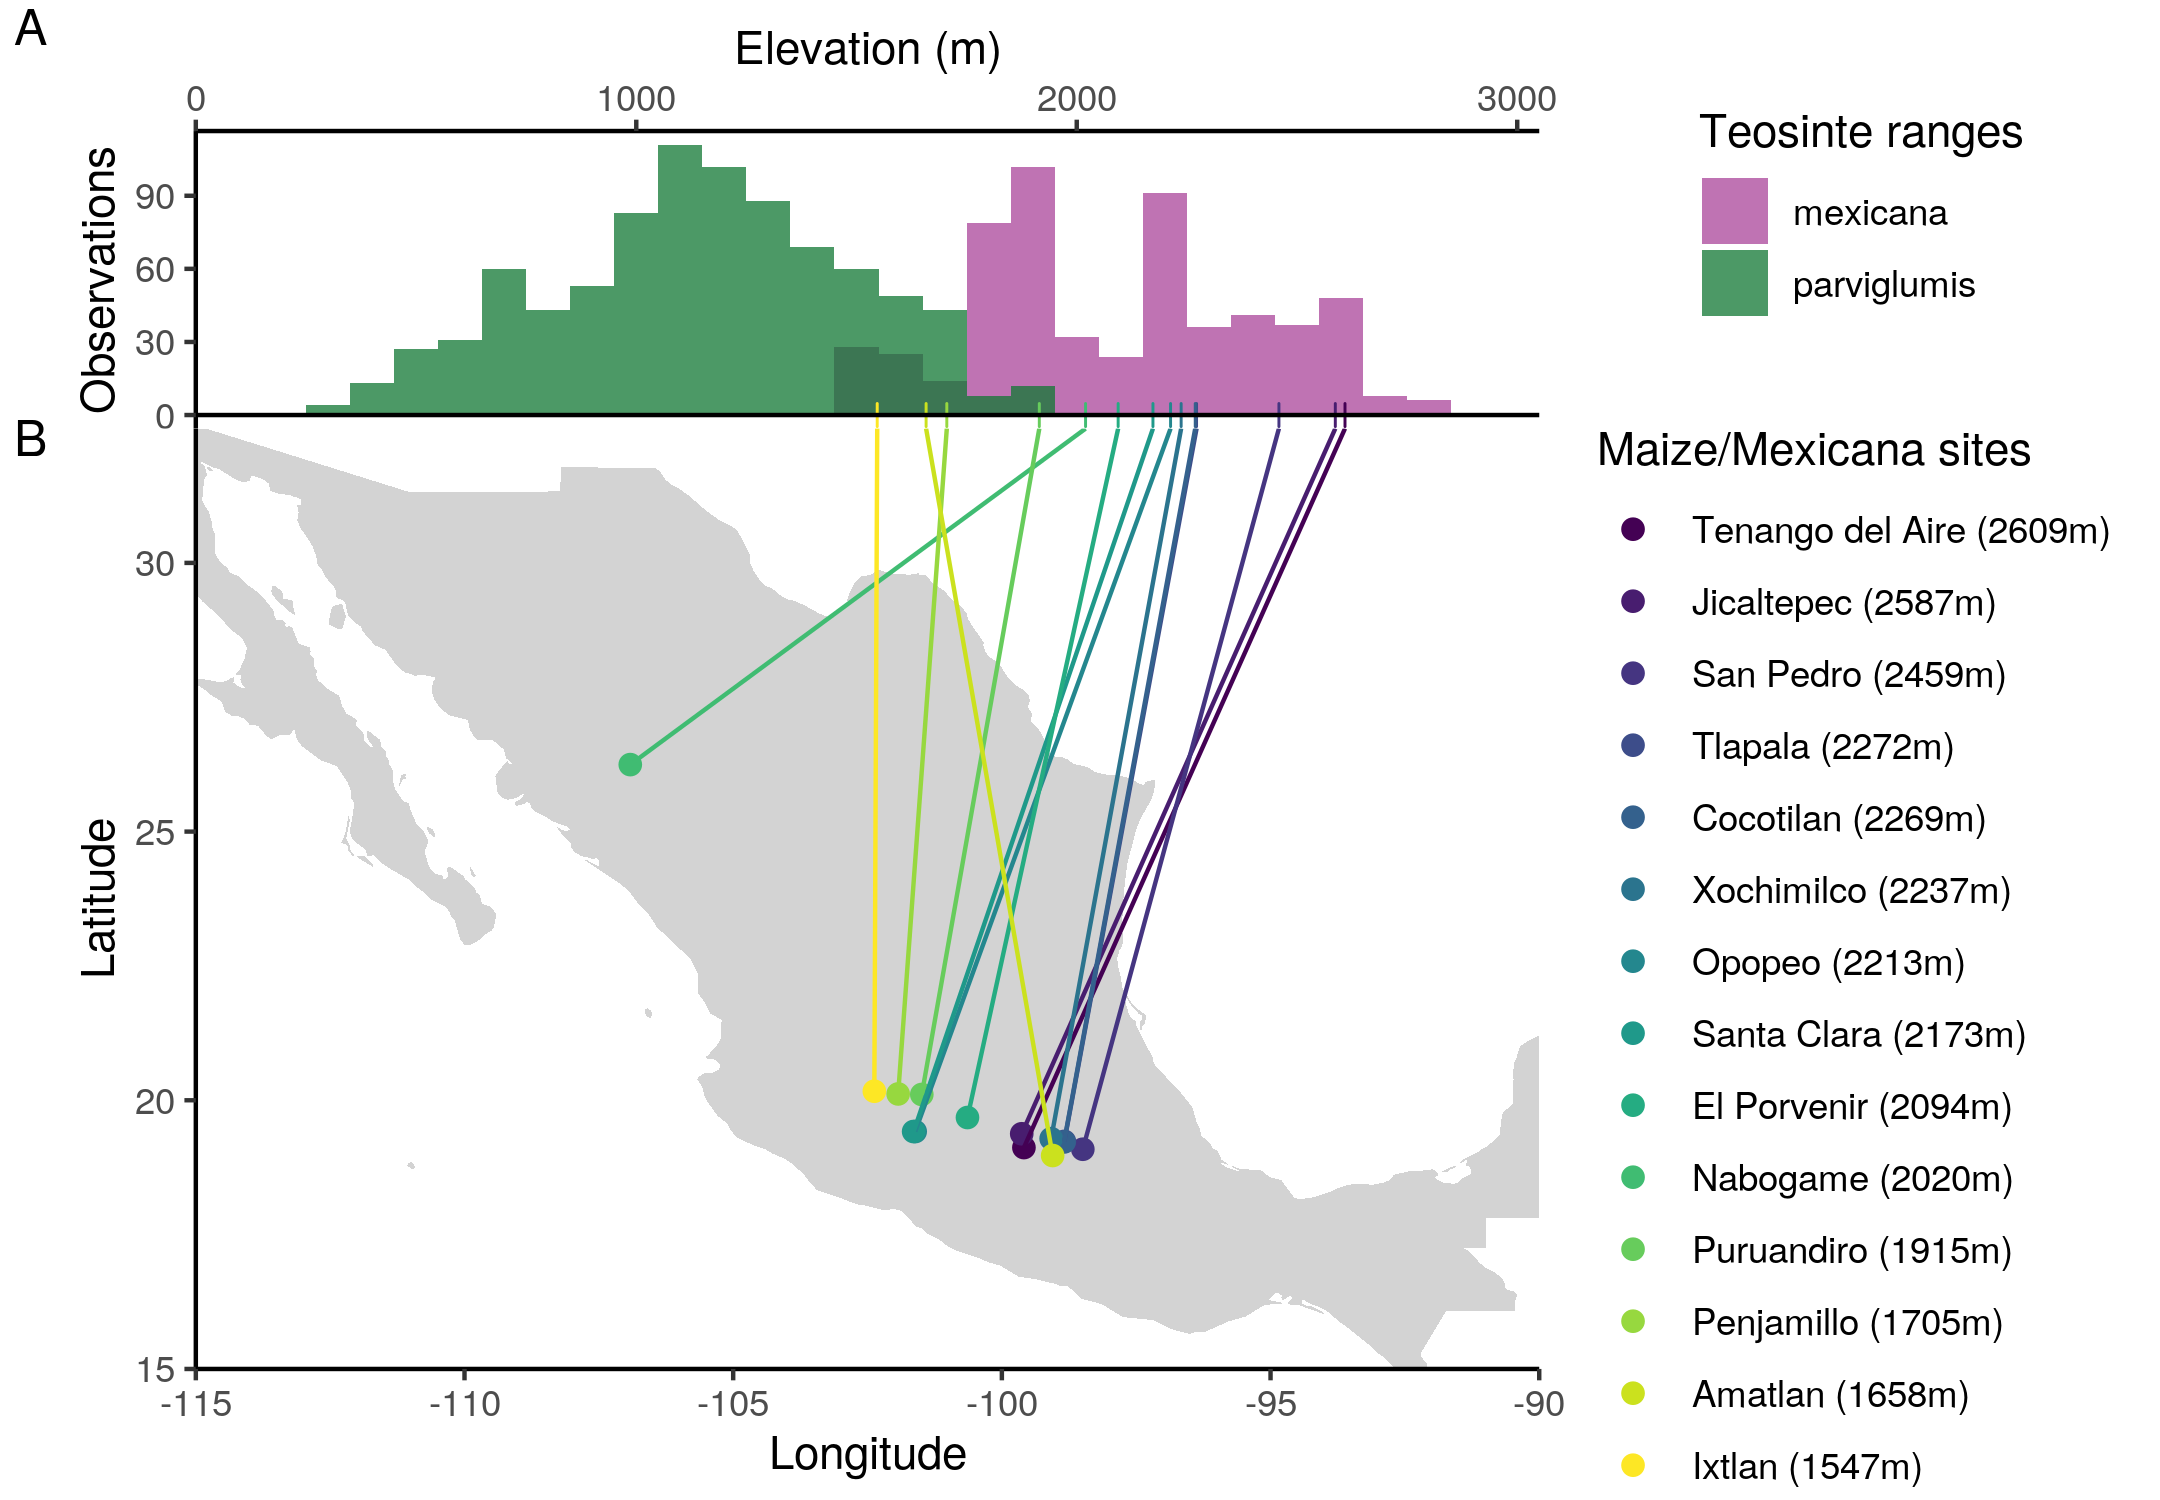
\includegraphics[width=\textwidth]{chapter2/figures/mexico_lines_elev_teo_color.png}
\caption{\color{Gray} \textbf{Sampled sympatric maize/\mexicana populations compared to distribution of teosintes} (A) Elevational range of teosintes based on historical occurrence data (1842-2016) from \cite{Gonzalez:2018}. (B) Geographic location and elevation of contemporary sympatric maize and \mexicana population pairs sampled across 14 sites in Mexico.}
\label{map}
\end{figure}

Principal components analysis of genetic diversity clearly separates maize and \mexicana, with putative admixed individuals from sympatric populations having intermediate values along PC1 (PCAngsd, Fig \ref{pca_maize_mex}). 

To estimate genomewide ancestry proportions for each individual, we ran NGSAdmix \cite{Skotte:2013_NGSadmix} with K=2 genetic clusters and genotype likelihoods for all maize and \mexicana individuals.
The two genetic clusters clearly map onto maize and \mexicana ancestry, with no indication of gene flow into the allopatric maize reference population but small amounts of maize ancestry in two of the three allopatric \mexicana populations (Fig \ref{global_anc_multi}A). 

Furthermore, we find a positive association between ancestry proportion and elevation (km), with higher \mexicana ancestry at higher elevations in both sympatric maize ($\beta=0.196, P = 1.42 \times 10^{-29}$) and sympatric \mexicana ($\beta=0.197, P = 4.38 \times 10^{-19}$) individuals (Fig \ref{global_anc_multi}B).

Increasing \mexicana ancestry at higher elevations is consistent with selection favoring \mexicana ancestry at higher elevations, but could also be due to purely demographic processes, e.g. a higher density of (wind-dispersed) \mexicana pollen at higher elevations, or increased gene flow from non-admixed maize populations at lower elevations. \ec{While most populations have admixture proportions well-predicted by their elevation, outlier populations may be the result of recent colonization histories for some locations or adaptation to other environmental niches. Within teosintes, elevation is a major axis of niche separation between \parviglumis (the ancestor of maize) and \mexicana \cite{Pyhajarvi:2013jc}, but genetic differentiation also correlates with soil nutrient content and at least four principal components constructed from climatic variables \cite{Aguirre-Liguori:2019}}.

%\begin{figure}[h!tb]
\begin{figure}[ht]
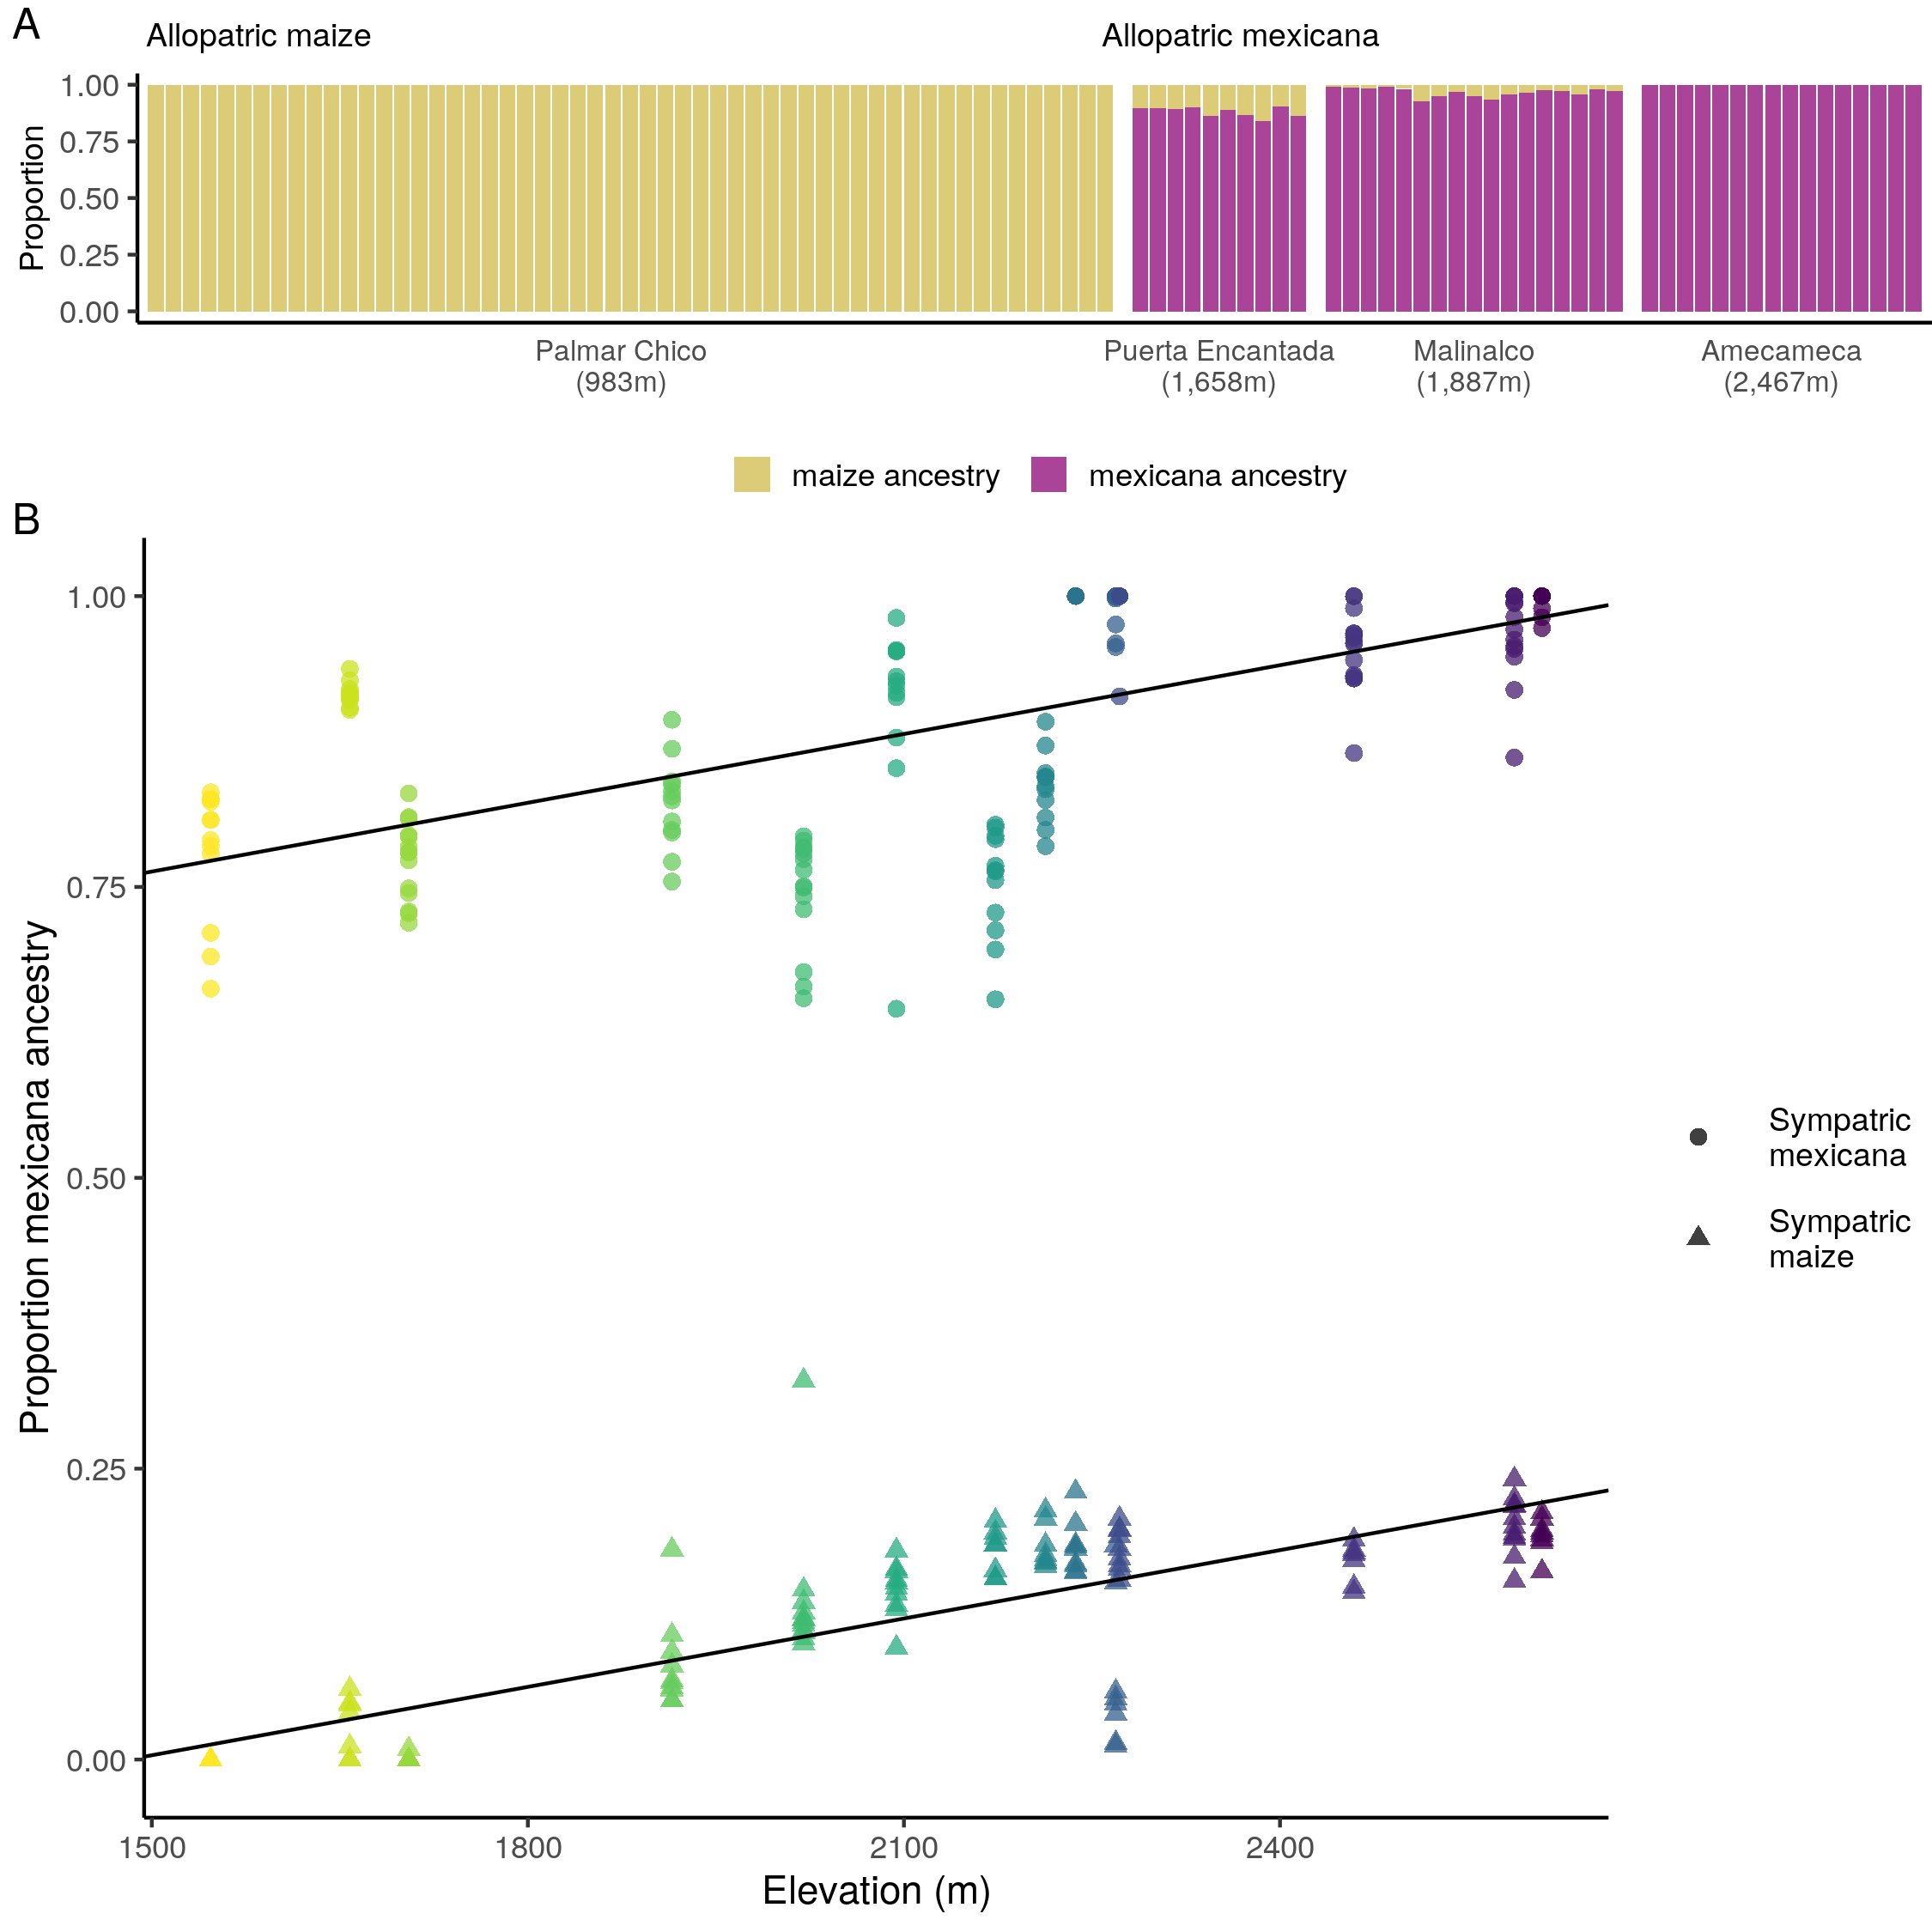
\includegraphics[width=\textwidth]{chapter2/figures/global_anc_multi.png}
\caption{\color{Gray} \textbf{Distribution of \mexicana ancestry by elevation} (A) Genomewide ancestry estimates (NGSAdmix) for allopatric maize and \mexicana reference individuals, grouped by sampling location. (B) Genomewide \mexicana ancestry estimates (NGSAdmix) for sympatric maize and \mexicana individuals (n = 305) along an elevational gradient, colored by sampling location. Lines show best linear model fit for \mexicana ancestry by elevation for each subspecies separately.}
\label{global_anc_multi}
\end{figure}

\subsection*{Origin and timing of introgression}
If \mexicana ancestry found in contemporary landrace genomes facilitated maize's colonization of the highlands approximately 6.2 thousands years ago \cite{Piperno:2001_highlands}, we would expect introgressed ancestry tracts to be short, due to many generations of recombination, and possibly to be derived from an ancient source population common to many present-day maize populations.
To test these predictions, we estimated local ancestry across the genome for individuals from each sympatric maize and \mexicana population using a hidden Markov model \ec{(HMM)} based on read counts (\cite{CorbettDetig:2017gh} see methods).
\ec{For each admixed population, this} \ec{HMM} simultaneously estimates local ancestry and, \ec{by optimizing the transition rate between different (hidden) ancestry states,} the generations since admixture.

Admixture is generally old, with median estimates of 1203 generations for sympatric maize populations and 718 generations for sympatric \mexicana populations (Fig \ref{time_admix}).

Because this HMM fits a single-pulse model to what was almost certainly multiple admixture events over time, we caution against over-interpretation of exact dates.
Multiple pulses or ongoing gene flow biases estimates towards the more recent pulse(s) \cite{Moorjani:2011_rolloff, Loh:2013_alder} and even old estimates do not exclude the possibility of limited more recent admixture.

These single-pulse approximations do, however, provide evidence that a large proportion of the introgression, especially into maize, is found on short ancestry tracts and therefore relatively old. 
%<<JEFF: is it worth text or supp. summary of ancestry tract lengths in cM? as a direct observation that is easy to intuit and supports this argument?>>

To identify likely source population(s) for introgressed ancestry, we compared $F_{ST}$ between all sympatric populations using only reads from high-confidence homozygous ancestry tracts (posterior $>$ 0.8) for maize and \mexicana ancestry separately.
We find that most \mexicana ancestry in maize resembles other \mexicana ancestry introgressed into other maize populations, rather that \mexicana ancestry from the local sympatric \mexicana population (Fig \ref{fst_within_ancestry}).
This finding is consistent with most introgressed ancestry being drawn from a communal source population, but none of the sympatric \mexicana populations have low enough $F_{ST}$ to tracts introgressed into maize to be a recent source.
While we cannot rule out recent introgression from an unsampled source population, the timing of our admixture estimates is more consistent with divergence of \mexicana ancestry, once introgressed into a maize background, from its original source population(s) (Fig \ref{time_admix}). Additionally, \mexicana ancestry tracts in maize have only slightly reduced genetic diversity ($\pi$, Fig \ref{pi_mexicana_ancestry_peaks}), meaning many \mexicana haplotypes have introgressed into maize at any given locus, with no evidence of a strong historical bottleneck.

\begin{figure}[ht]
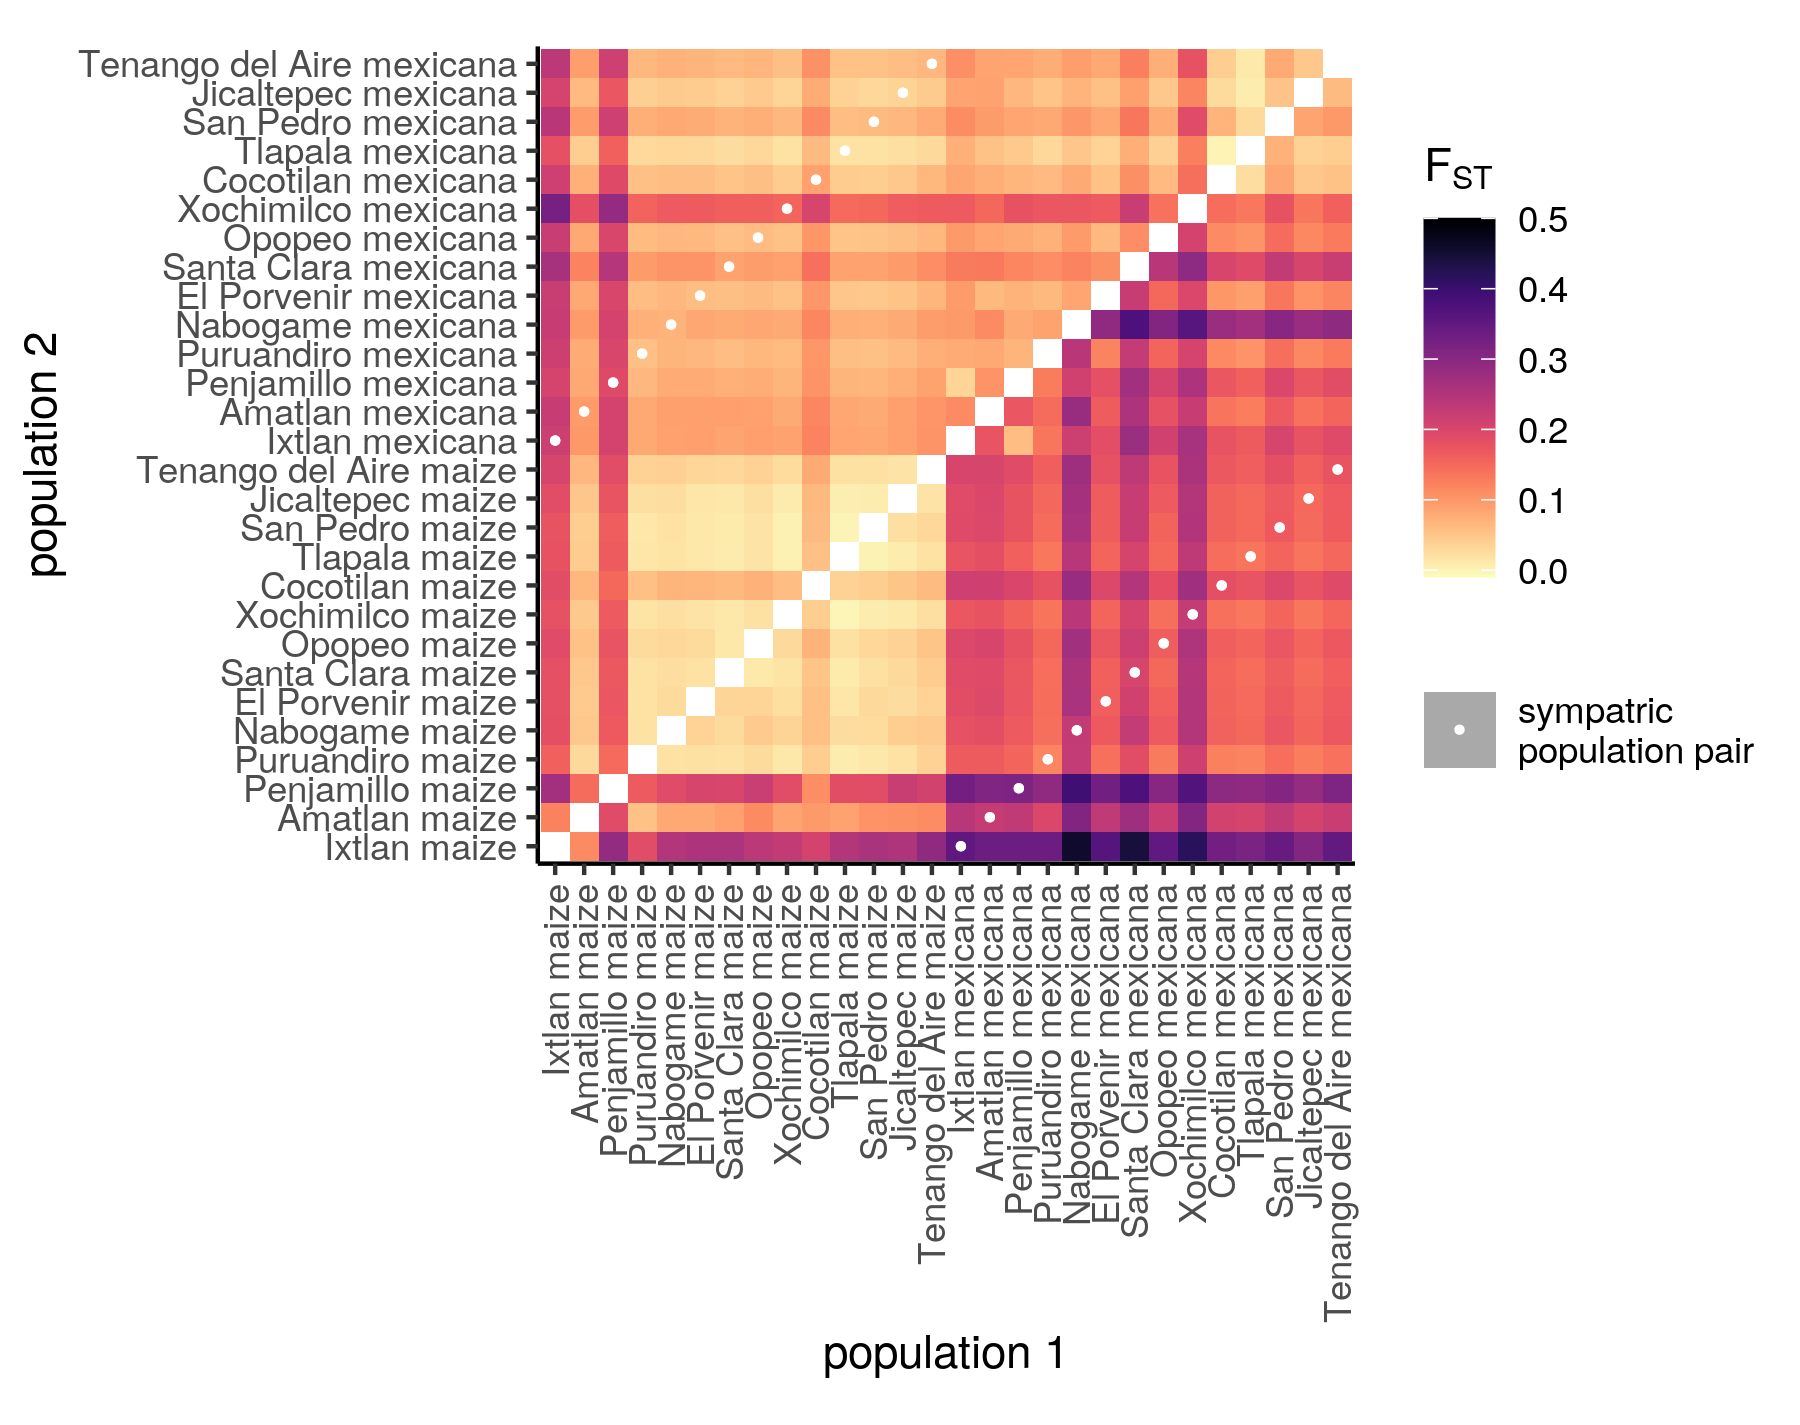
\includegraphics[width=\textwidth]{chapter2/figures/fst_within_maize_or_mexicana_ancestry_genomewide_heatmap_both.png}
\caption{\color{Gray} \textbf{$F_{ST}$ between ancestry tracts from different populations} 
Pairwise $F_{ST}$ between maize ancestry tracts from population 1 (x-axis) and population 2 (y-axis) are shown in the upper left triangle, while $F_{ST}$ estimates for \mexicana ancestry tracts are shown in the lower right triangle. 
Populations are sorted by subspecies, then elevation. Local sympatric maize-\mexicana population pairs are highlighted with a white dot \ec{and do not show reduced $F_{ST}$ relative to other (non-local) maize-\mexicana comparisons. 
Additionally, introgressed \mexicana ancestry shows low differentiation between maize populations (creating a light-colored maize block in the lower right triangle) and no potential \mexicana source populations show especially low $F_{ST}$ with this block.
%In addition, the light-colored maize corner in the lower right triangle shows that introgressed \mexicana ancestry has low differentiation between maize populations, consistent with shared drift post-admixture, but no potential \mexicana source populations show especially low $F_{ST}$ with this corner. 
Light coloring generally across the upper left triangle reflects the low differentiation within maize, providing little information to distinguish between potential maize ancestry sources.}}
\label{fst_within_ancestry}
\end{figure}

Two lower elevation maize populations are an exception to this general pattern: Ixtlan and Penjamillo. These populations have higher $F_{ST}$ between their introgressed ancestry tracts and other \mexicana tracts in maize \ec{(Fig \ref{fst_within_ancestry})}, more recent timing of admixture estimates \ec{(Fig \ref{time_admix})}, and reduced genetic diversity (Figs \ref{pi_mexicana_ancestry_peaks}-\ref{pi_maize_ancestry}).
These patterns could be caused by small population sizes and more recent independent admixture, although $F_{ST}$ does not identify a likely \mexicana source population.
Consistent with this interpretation, we have evidence that local maize at Ixtlan is at least partially descended from recently introduced commercial seed (relayed by local farmers \cite{Hufford:2013_crop_wild}). 

The lack of a clear reduction in $F_{ST}$ for \mexicana ancestry tracts between sympatric population pairs, combined with older timing of admixture estimates, indicates that while contemporary hybridization may occur in the field between maize crops and adjacent  \mexicana populations, this is not the source for the bulk of the introgressed ancestry segregating in highland maize. 

Instead, we propose that the majority of \mexicana ancestry in maize derives from admixture over 1000 years ago, possibly from a diverse set of \mexicana source populations over a large geographic and temporal span, and the resulting ancestry tracts are now distributed across different contemporary maize populations.
These genomewide average $F_{ST}$ results, however, do not exclude the possibility that particular regions were introgressed from one or more distinct, possibly local, source populations.

While we also analyzed $F_{ST}$ within high-confidence maize ancestry tracts, we found that maize ancestry is too homogeneous to make inferences about potential admixture source populations of maize into \mexicana (Figs \ref{fst_within_ancestry}, \ref{pi_maize_ancestry}). 

\subsection*{Selection against introgression genomewide} 
When there is widespread selection against introgressing variants at many loci across the genome, selection will more efficiently remove linked ancestry in regions of the genome with lower recombination rates, which creates a positive relationship between local recombination rate and the proportion of introgressed ancestry \cite{Veller:2019ge, Schumer:2018hc, Harris:2016fp, Juric:2016jj, Sankararaman:2014_neanderthals, Brandvain:2014cq, Aeschbacher:2017_mimulus, Kenney_Sweigart:2016_mimulus, Nelson:2021_mimulus, Martin:2019_butterflies, Edelman:2019_butterfly}.
To test whether such negative selection is shaping patterns of introgression genomewide in sympatric maize and \mexicana, we first divided the genome into quintiles based on the local recombination rates for 1 cM windows. 
We then ran NGSAdmix on the SNPs within each quintile separately, using K=2 clusters, to estimate maize and \mexicana ancestry proportions. We used a recombination map from maize \cite{Ogut:2015df}, which is likely to be correlated with other \textit{Zea} subspecies at least at the level of genomic quintiles, but a limitation of this analysis is that we do not have a recombination map for hybrid populations which means that e.g. segregating structural inversions will not necessarily show low recombination rates.

Our results from sympatric maize landraces are consistent with selection against \textit{mexicana} introgression at many loci genomewide, resulting in lower introgressed ancestry in regions of the genome with lower recombination rates (Fig \ref{K2_by_r}A). 
We find a positive Spearman's rank correlation between recombination rate quintile and mean introgressed \mexicana ancestry proportion ($\rho = 1,\ \text{CI}_{95}[0.85,\ 1.00]$), \ec{reflecting the fact that introgression increases monotonically across quintiles.}  \ec{A} similar analysis using $f_4$ statistics replicates this result (see methods, Fig \ref{f4_tree}-\ref{f4_maize_by_cd} and \nameref{spearmans_rho_f4_sympatric_maize_pop22}). The higher elevation maize populations show this pattern most starkly; while all individuals have low \mexicana ancestry for the lowest recombination rate quintile, some high elevation populations have individuals with over 40\% introgressed ancestry for the highest recombination rate quintile (Fig \ref{K2_by_r}B). Using a linear-model fit, we found a significant interaction between recombination rate quintile and the slope of ancestry across elevation in sympatric maize (\nameref{tbl_elev_r_interaction_5}). 
This is again consistent with low-recombination rate regions having a stronger effect of linked selection reducing \mexicana ancestry, with higher elevation maize landraces either experiencing larger amounts of gene flow or retaining more ancestry due to adaptive processes in high recombination regions (Fig \ref{K2_by_r_elev_lm}).


\begin{figure}[ht]
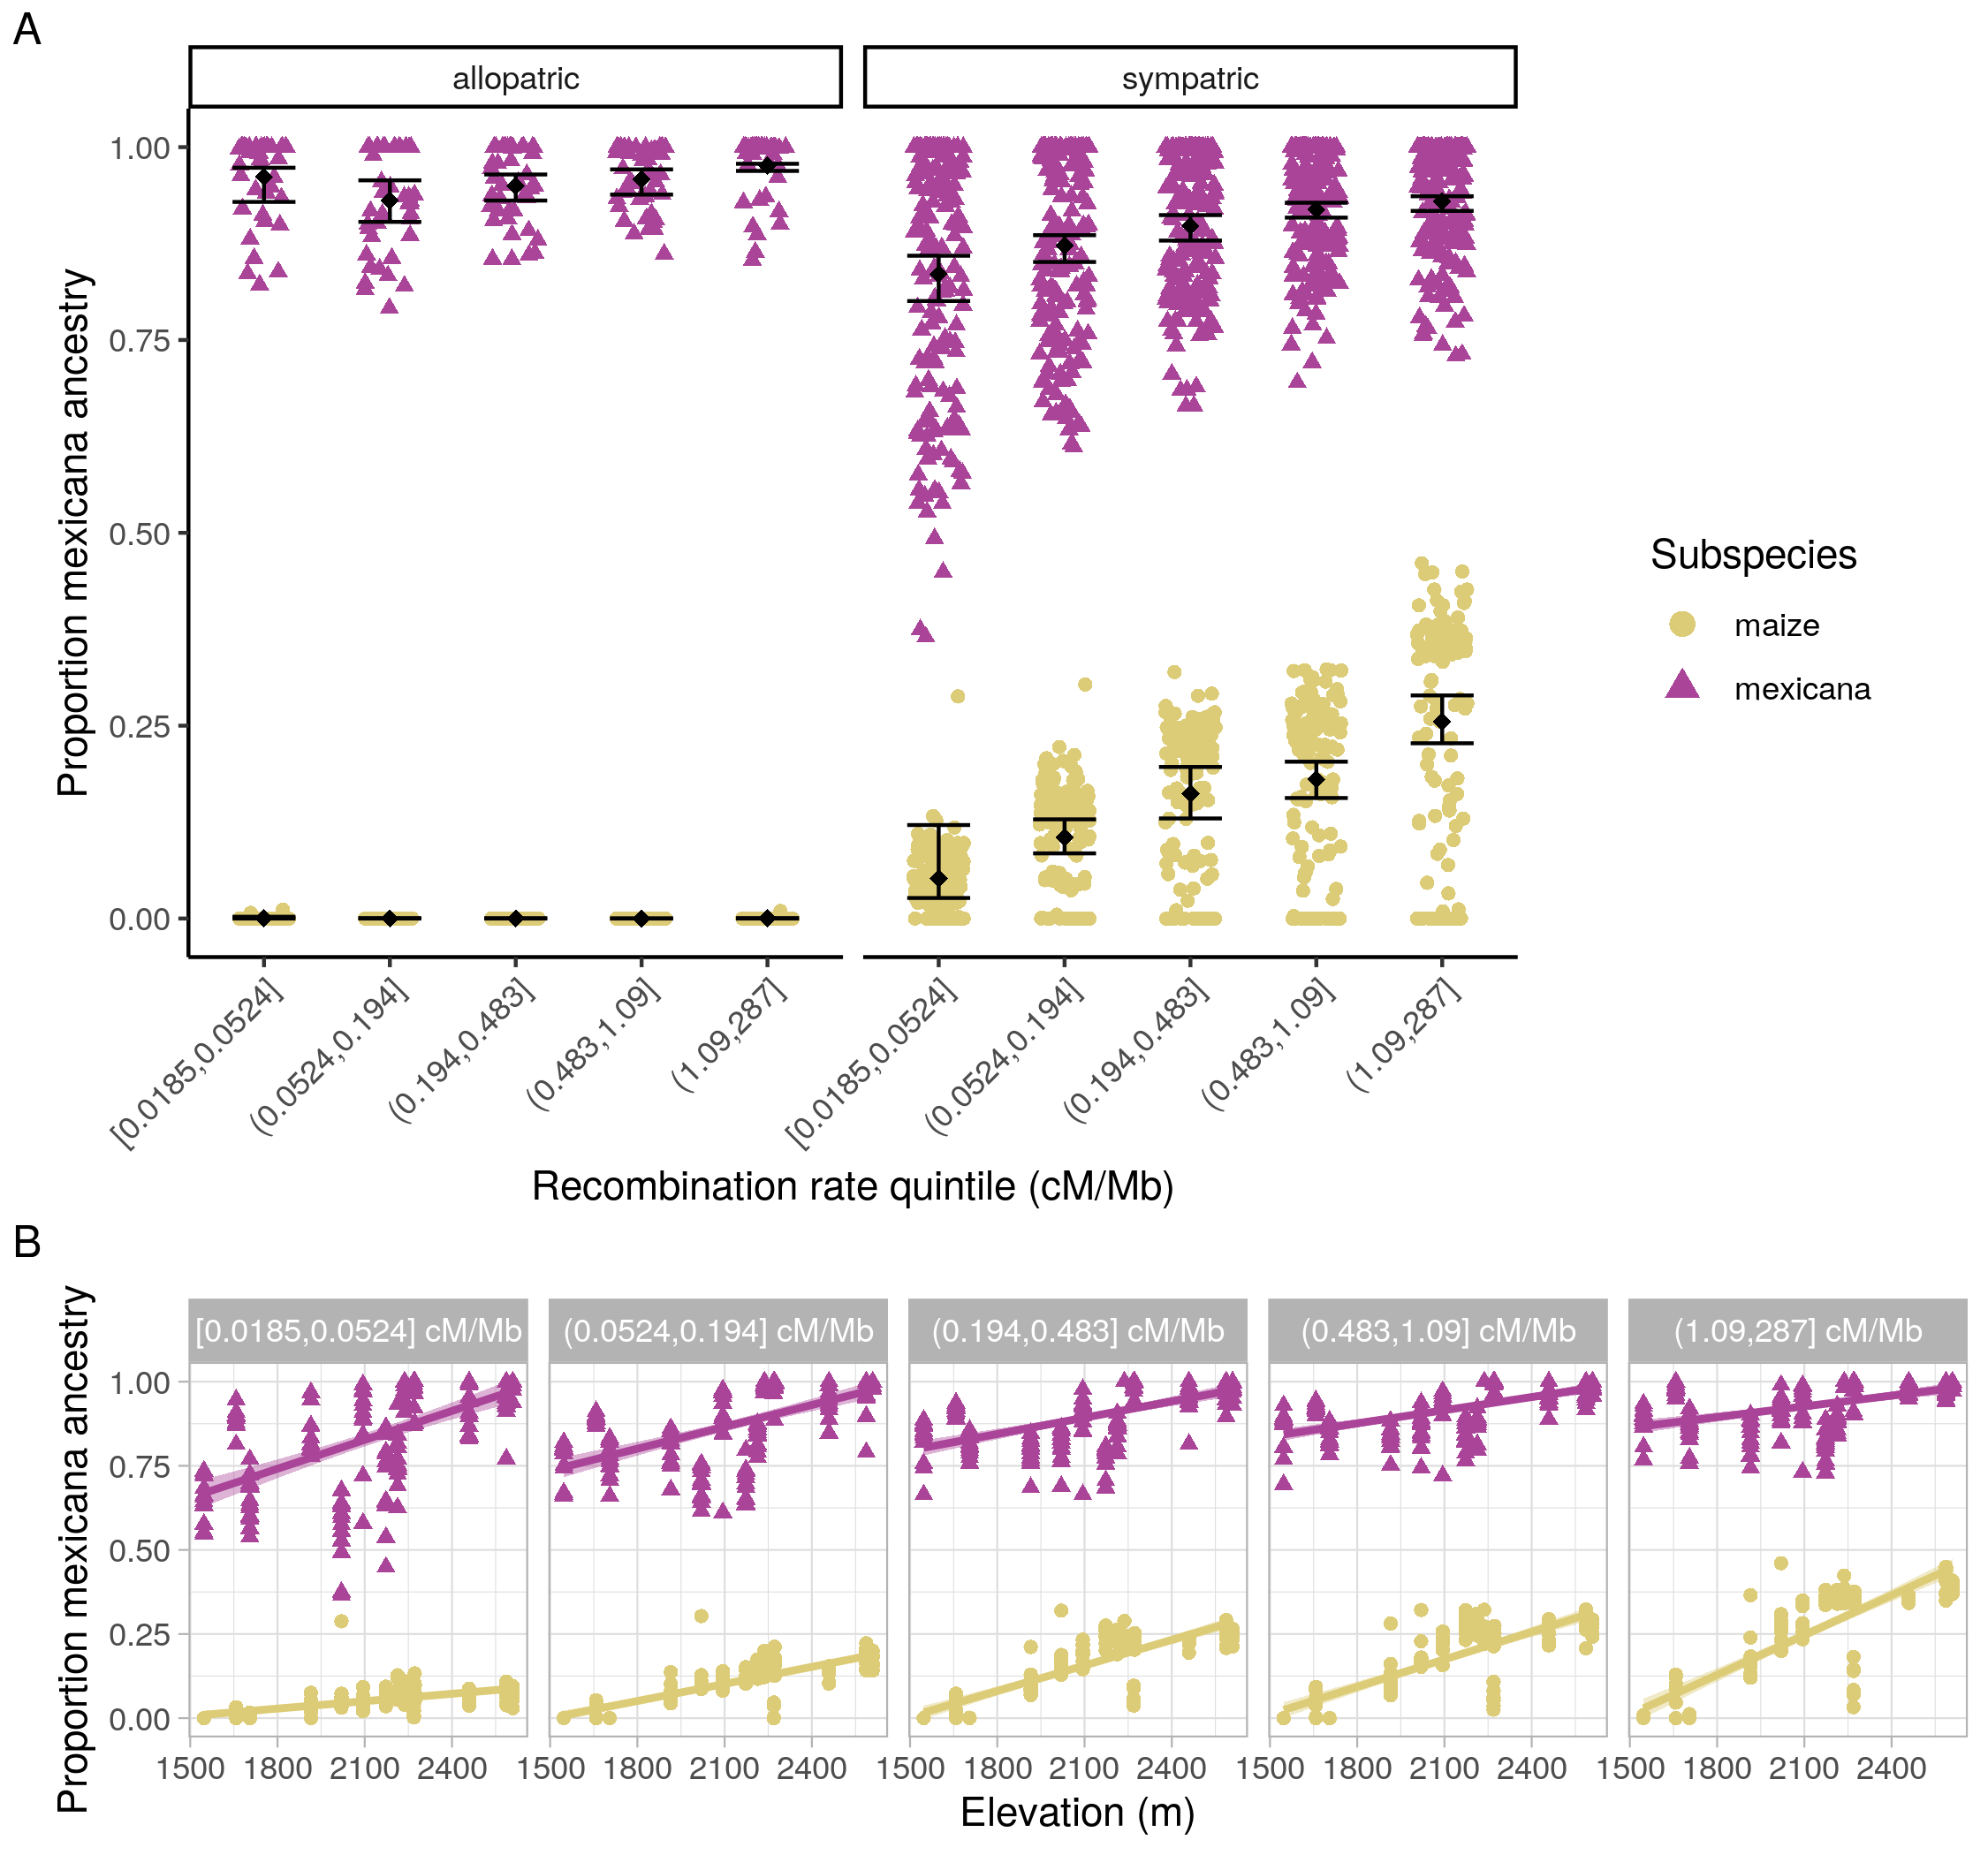
\includegraphics[width=.95\textwidth]{chapter2/figures/K2_by_r_multi_panel.png}
\caption{\color{Gray} \textbf{(A) \textit{Mexicana} ancestry by recombination rate}. Inferred \mexicana ancestry in  allopatric reference populations (left) and sympatric maize and \mexicana populations (right) using NGSAdmix (K=2) by recombination rate quintiles. Group mean and 95\% confidence interval based on bootstrap percentiles (n = 100) are depicted in black. Ancestry estimates for each individual are shown as points, colored by subspecies, and points are jittered for better visualization. (B) Slopes of \mexicana ancestry across elevation for each recombination rate quintile, based on NGSAdmix estimates. Each point is a sympatric maize or \mexicana individual and lines show the best-fit linear model for ancestry by elevation (with shaded 95\% confidence interval) estimated separately for each quintile and subspecies.}
\label{K2_by_r}
\end{figure} 

Because recombination rate is positively correlated with gene density in \textit{Zea} \cite{Schnable:2009_B73}, we also tested the Spearman's rank correlation between quintiles defined by coding base pairs per cM and their proportion introgressed \mexicana ancestry. 
Again we found evidence supporting pervasive selection against introgression (Fig \ref{K2_by_cd}, $\rho = -1,\ \text{CI}_{95}[-1,\ -0.85]$).

In contrast, sympatric \mexicana shows an unexpected negative relationship between recombination rate and introgression from maize, with more \mexicana ancestry (lower introgression) in the highest recombination rate regions of the genome ($\rho = 1,\ \text{CI}_{95}[0.9,\ 1]$). Correlations with coding bp per cM and based on $f_4$ statistics corroborate this pattern (see \ref{K2_by_cd}-\ref{f4_mexicana_by_cd} and \nameref{spearmans_rho_f4_sympatric_mexicana_pop22}). 
While one possible explanation is that introgressing maize ancestry is overall beneficial, not deleterious, a similar pattern could also be produced from a number of different distributions of fitness effects for maize alleles, including for example if most maize alleles are deleterious but some have strong beneficial consequences.
While maize ancestry in general is not predicted to provide adaptive benefits in teosinte, invasive \mexicana in Europe shows selective sweeps for maize ancestry at multiple loci that have contributed to its establishment as a noxious weed \cite{Le_Corre:2020} and we speculate that maize could be a source of alleles adapted to human-modified landscapes.

We repeated these analyses using local ancestry calls as our introgression estimates and found a non-significant Spearman's rank correlation between \mexicana ancestry and recombination rates for 1 cM windows in sympatric maize (Fig \ref{local_ancestry_mexicana_by_log10r}, $\rho = 0.011,\ \text{CI}_{95}[-0.039,\ 0.062]$) and a negative rank correlation between \mexicana ancestry and recombination rate in sympatric \mexicana ($\rho = -0.473,\ \text{CI}_{95}[-0.512,\ -0.432]$).
Contrasting results between global and local ancestry methods could be a reflection of true evolutionary differences across different time periods; local ancestry methods capture patterns from more recent gene flow that comes in longer ancestry blocks while STRUCTURE-like algorithms (NGSAdmix) and $f_4$ statistics are based on allele frequencies that collapse information across ancestry blocks of any size, capturing a longer evolutionary time scale.
This interpretation would suggest that \mexicana has experienced stronger selection against more recent maize gene flow than historical gene flow. 
%\jri{<<JEFF:we can test this? maybe come back to to test formally?} 
However, we caution that local ancestry methods may also have subtle biases in power that are sensitive to local recombination rates and make them less reliable for comparing ancestry patterns across recombination rate quintiles.

Overall, we find support for widespread selection against introgression into maize and mixed results from similar tests of this hypothesis in \mexicana.

\subsection*{High introgression peaks shared across populations}

To assess adaptive introgression in our sympatric populations, we identified introgression ‘peaks' where minor ancestry exceeds the genomewide mean by more than 2 standard deviations. We find no strong reduction in average diversity ($\pi$) for \mexicana ancestry at high introgression peaks (Fig \ref{pi_mexicana_ancestry_peaks}). 
This maintenance of diversity implies that selection at most peaks has favored multiple \mexicana haplotypes, and hard sweeps for a recent beneficial mutations on a specific haplotype are rare.

We observe that many high \textit{mexicana} ancestry peaks are shared across subsets of our 14 maize landrace populations (see e.g. chr4, Fig \ref{maize_chr4}). 
While most outlier peaks are unique to a single population, many peaks are shared across 7 or more of the populations (Fig \ref{combmatrix_peaks_maize}).
To a lesser extent, we also observe sharing of high-introgression peaks for maize ancestry in sympatric \mexicana populations (Fig \ref{combmatrix_peaks_mexicana}).

\begin{figure}[ht]
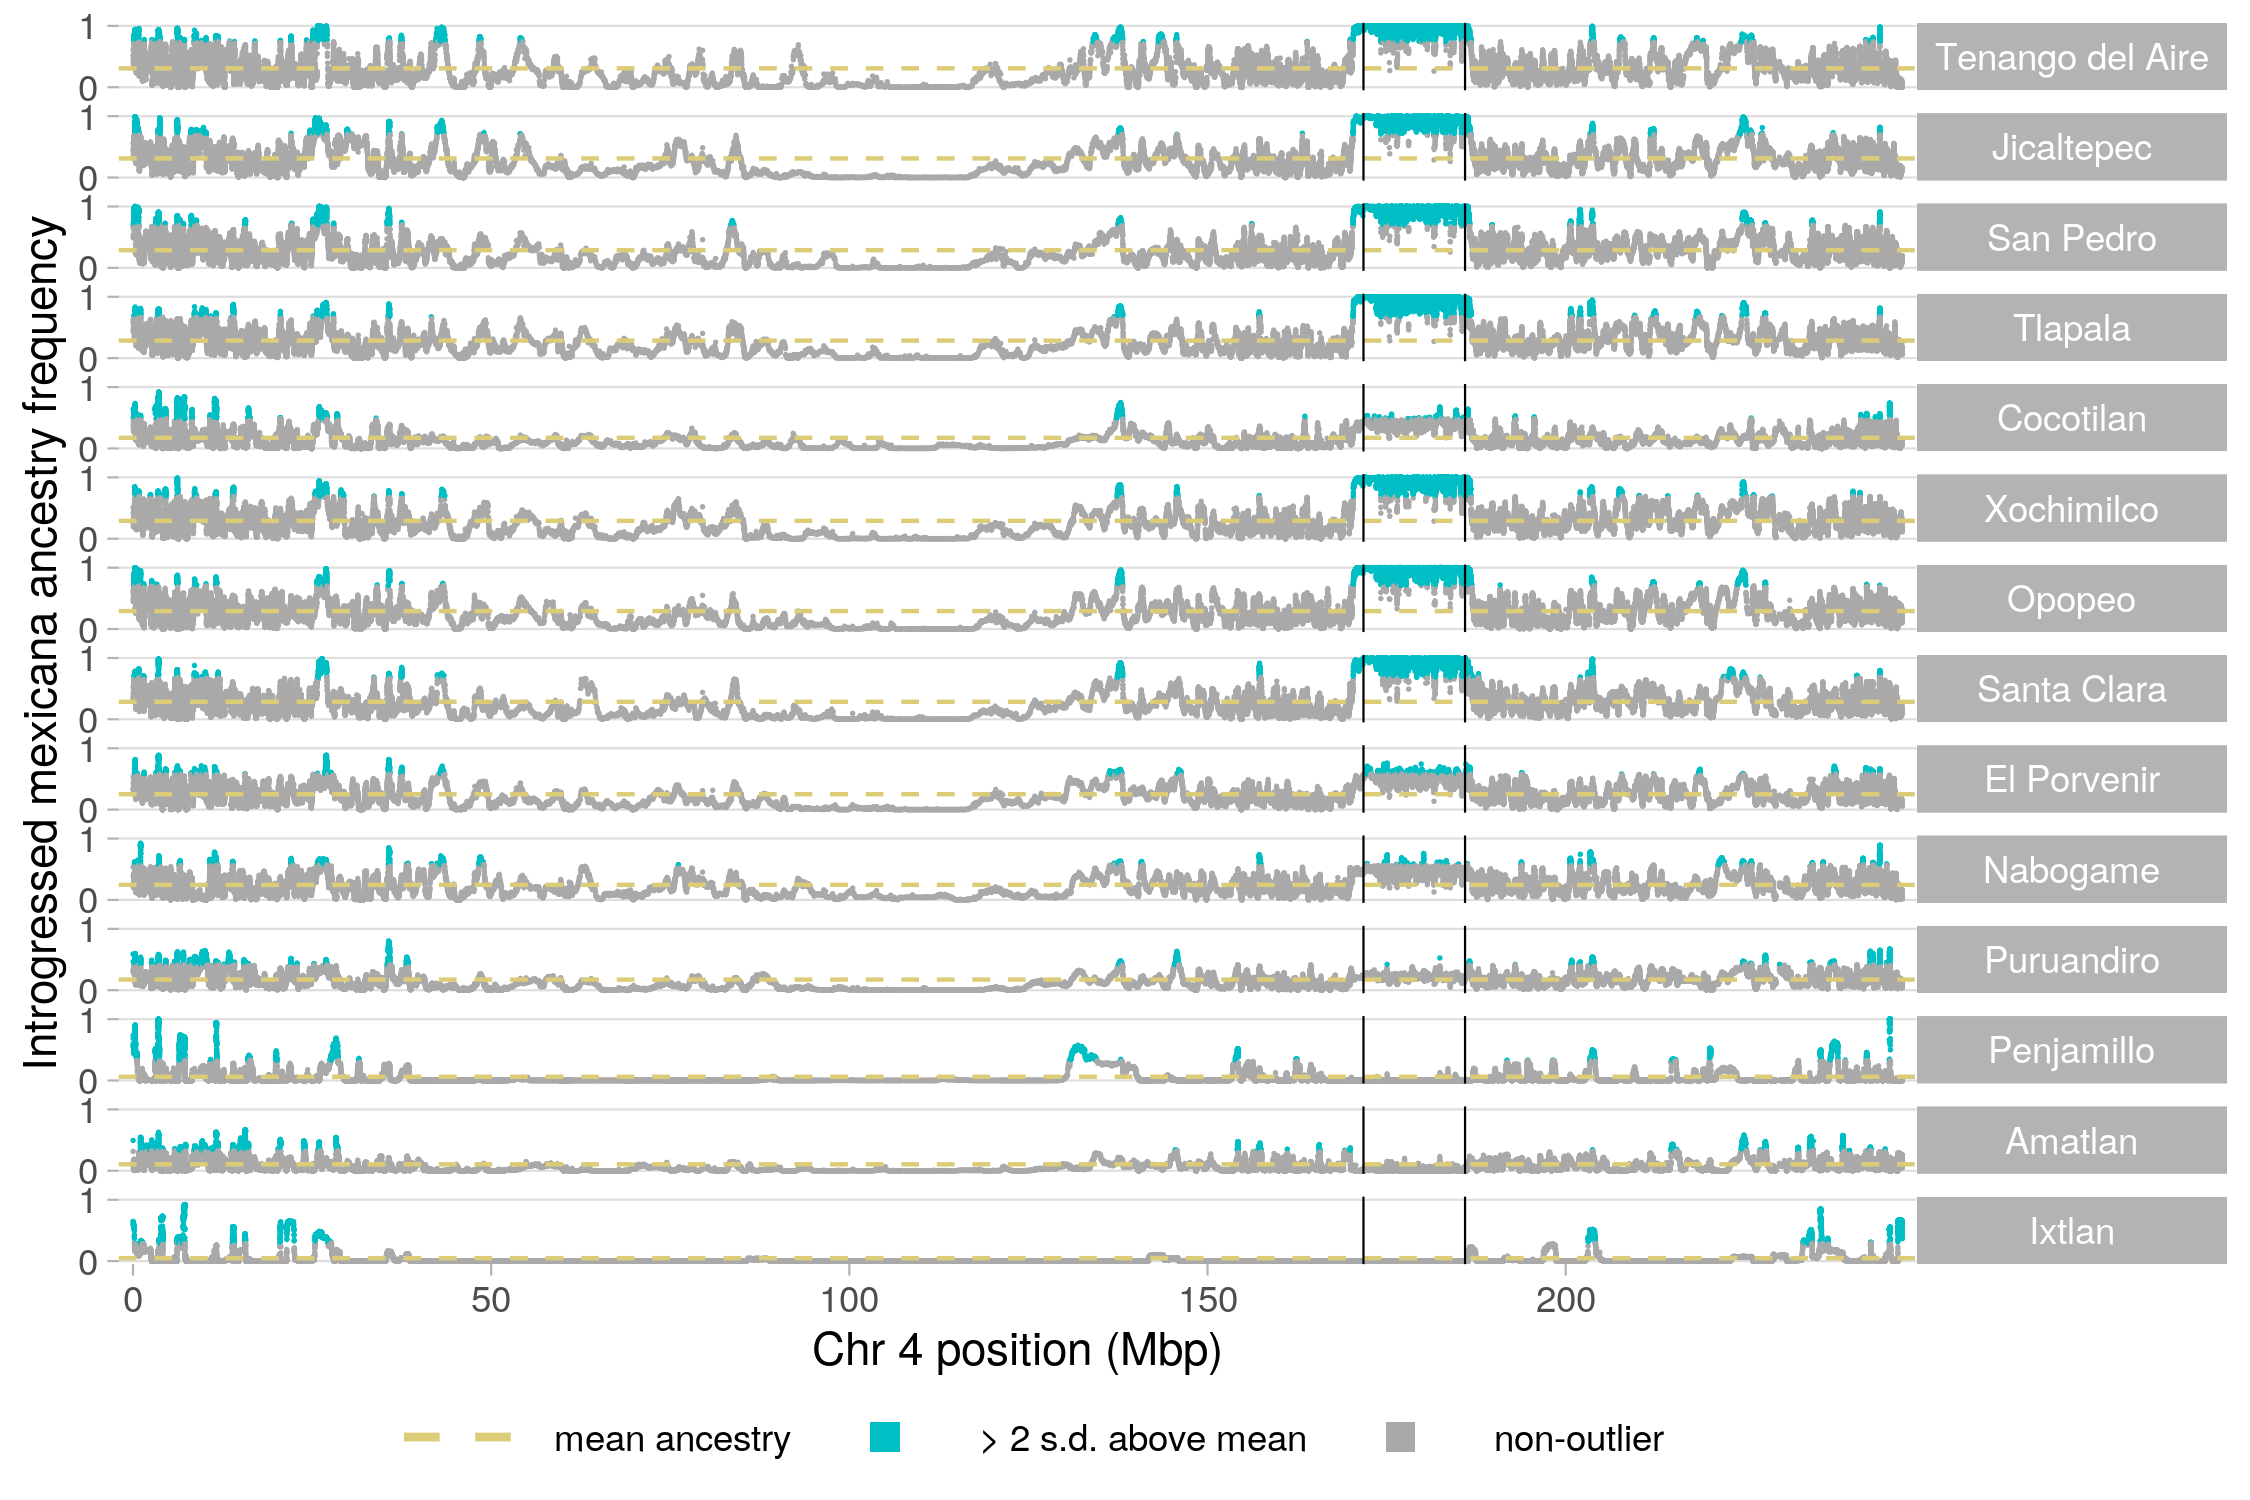
\includegraphics[width=.95\textwidth]{chapter2/figures/maize_shared_outliers_chr_4.png}
\caption{\color{Gray} \textbf{Introgression in maize landrace populations across chromosome 4}. Local introgressed ancestry frequency for each maize landrace population compared to their genomewide mean. Populations are ordered from high to low elevation (top to bottom). High introgression peaks with more than 2 standard deviations above the population mean introgressed \mexicana ancestry are highlighted in blue. Vertical black lines show the previously identified endpoints for a large inversion (\textit{Inv4m} coordinates from Fig 3 of \cite{Pyhajarvi:2013jc}). For local ancestry on other chromosomes \ec{and for sympatric \mexicana}, see Figs \ref{maize_chr1}-\ref{mexicana_chr10}}. 
\label{maize_chr4}
\end{figure}
% Turelli wants low to high elevation on side of plot
High introgression peaks in many independent populations would be very unexpected by chance. However, our sampled populations do not provide independent evidence for adaptive introgression, due to shared gene flow and drift post-admixture (e.g. long-distance human-assisted dispersal of maize seed). To estimate the rate of peak sharing we should expect from demographic processes alone, we simulated 100,000 unlinked loci under a multivariate normal distribution parameterized with the empirical ancestry variance-covariance matrix K (see methods). 
These simulations preserve the ancestry variance across loci within populations and non-independence in ancestry between populations.

For both sympatric maize and \mexicana, every population shares an excess of high introgression peaks with all other populations compared to expectations set by our MVN null model. 
However, peak sharing is most elevated among high elevation maize populations (with the exception of Cocotilan, see Fig \ref{network_peaks}). 
To investigate the origins of population-specific peaks of introgression, we calculated $F_{ST}$ between homozygous \mexicana ancestry in local maize and in each \mexicana population for these genomic regions.
Patterns of $F_{ST}$ between local sympatric pairs at local introgression peaks differed little from background $F_{ST}$ (Fig \ref{local_fst_peaks}), offering little support for the idea that population-specific peaks arose from recent, locally sourced, adaptive introgression.
Instead, patterns in maize are consistent with introgressed \mexicana ancestry tracts from old shared admixture being favored by natural selection, and thus rising to high frequency, in a subset of landraces. 
% I changed this wording because it wasn't accurate with the figure! We didn't compare local vs. non-local fst at peaks. Instead we compared local fst at peaks vs. non-peaks.

\begin{figure}[ht]
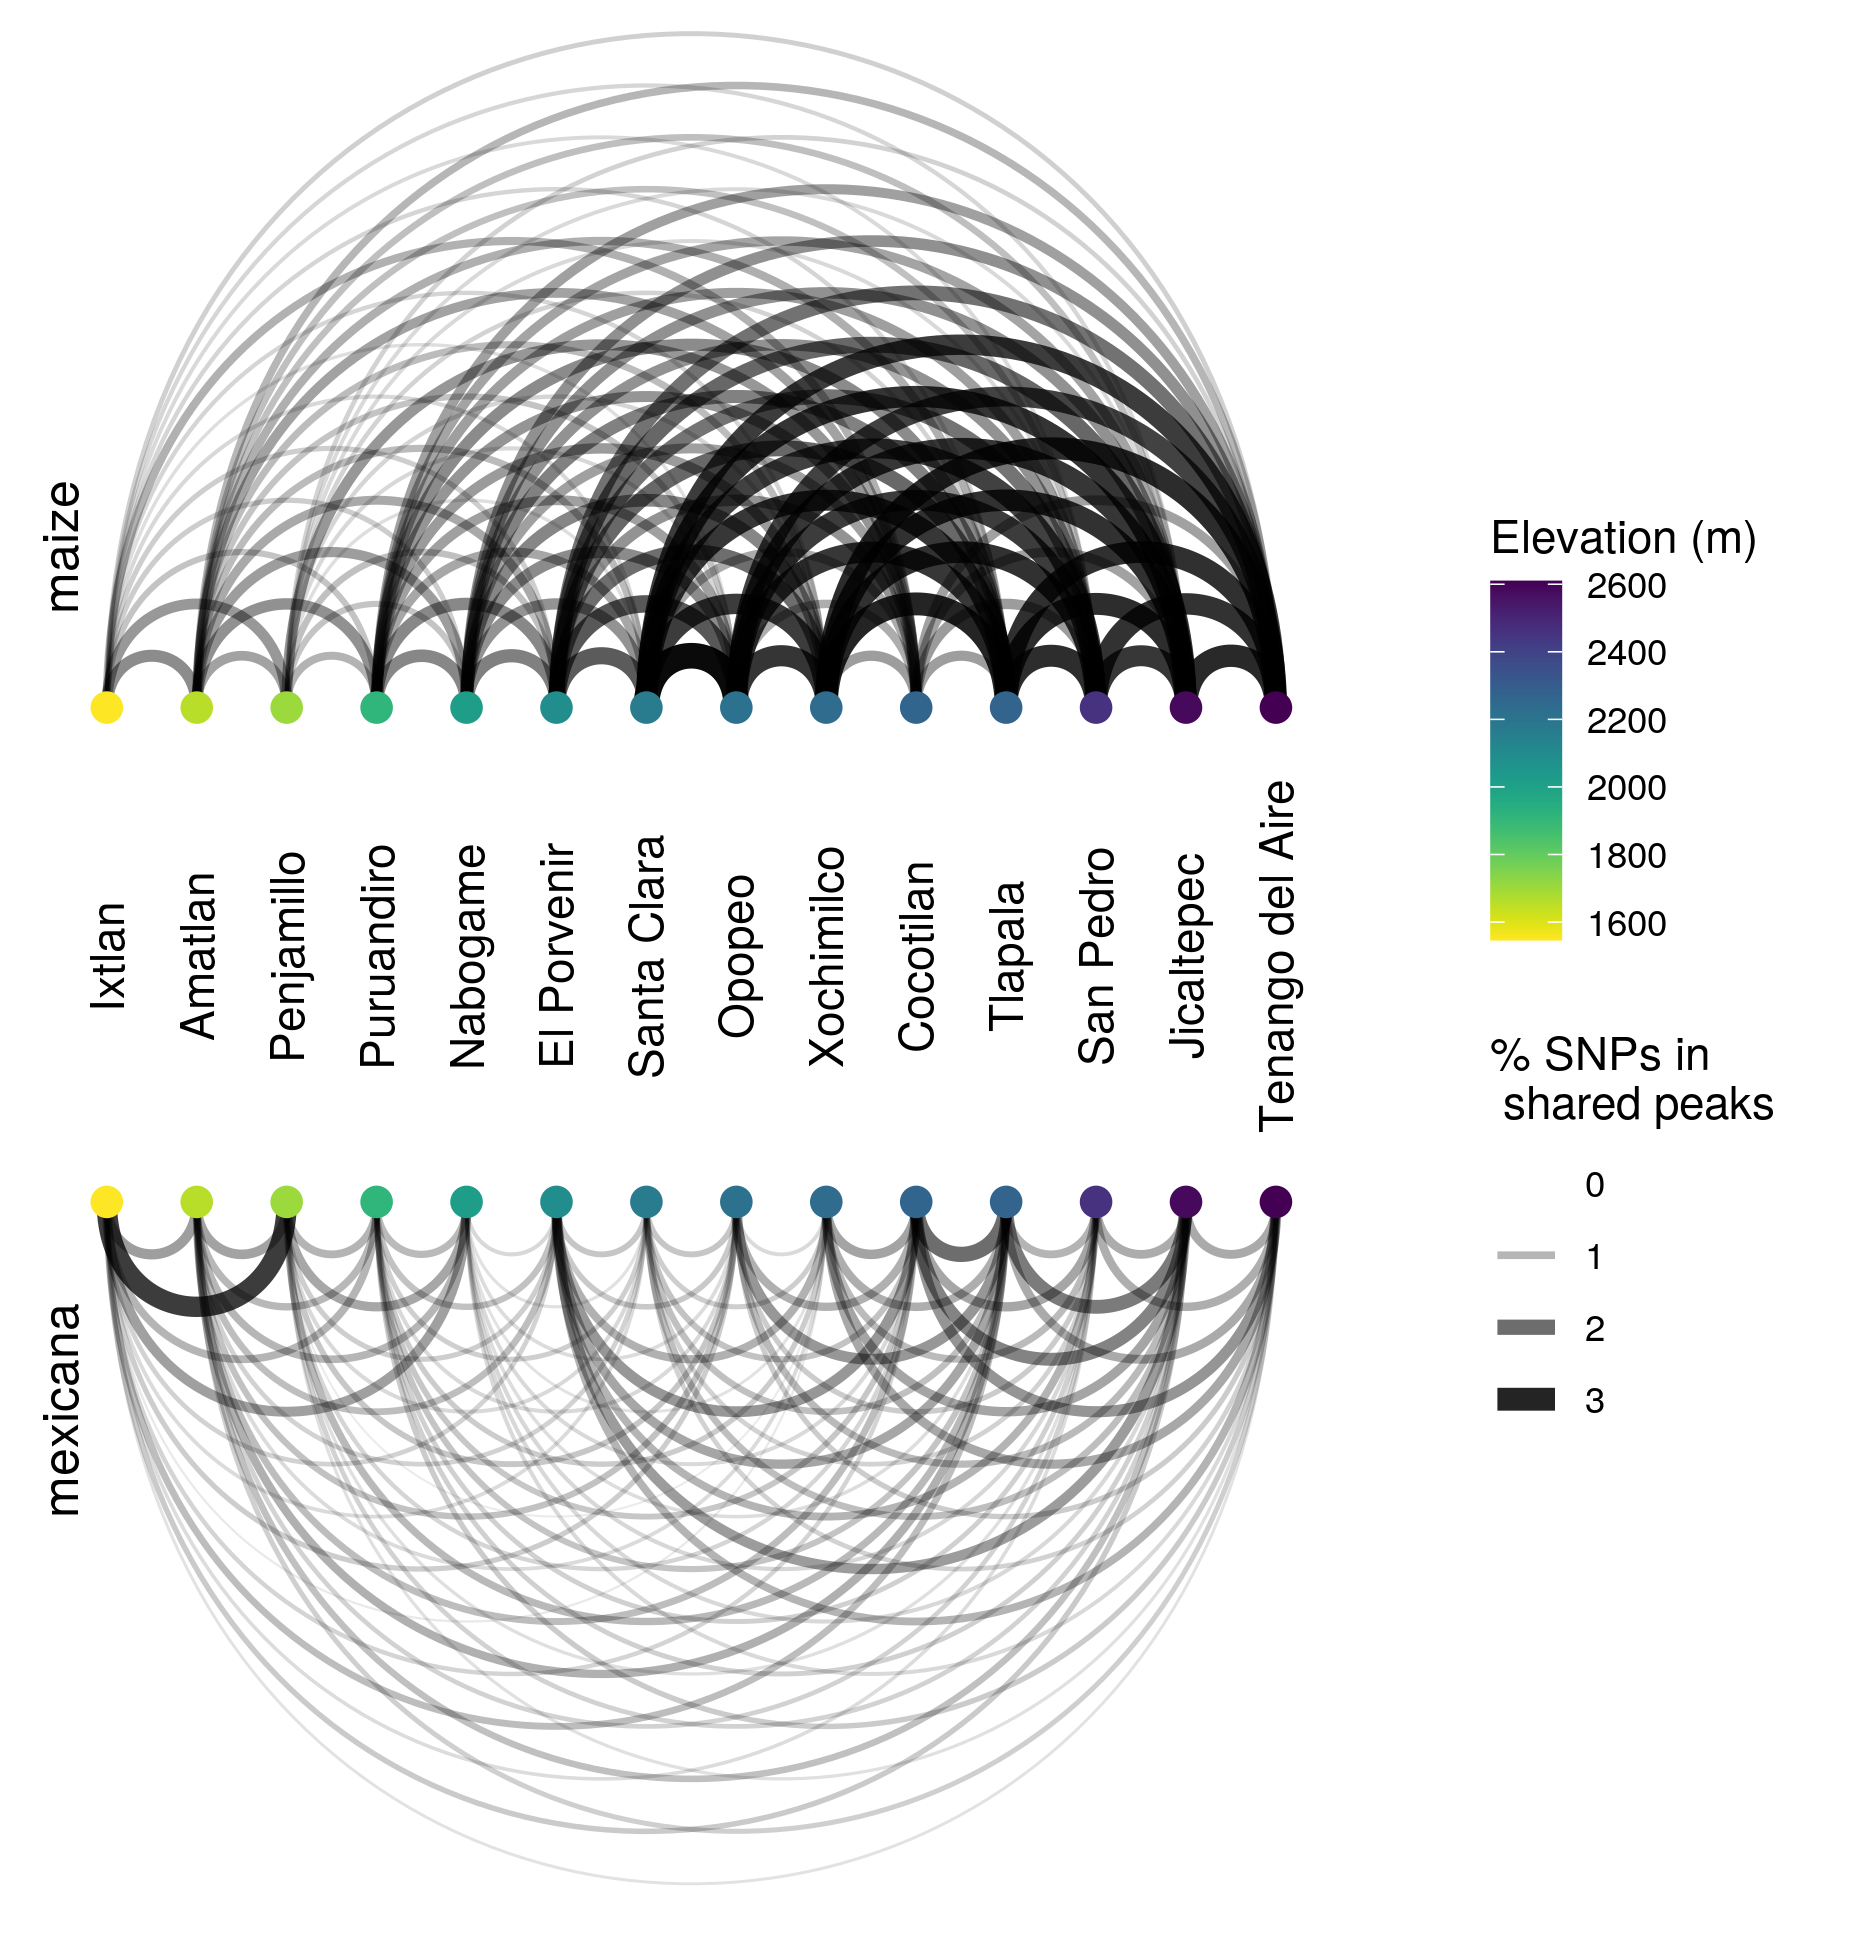
\includegraphics[width=.9\textwidth]{chapter2/figures/network_peak_sharing_data_only.png}
\caption{\color{Gray} \textbf{Introgression peaks shared across populations} Networks for sympatric maize (top) and \mexicana (bottom), where each node is a sampled population labelled by location and ordered by elevation. 
Edges connecting a pair of populations represent the percent of SNPs within shared ancestry peaks (introgressed ancestry $>$ 2 s.d. above each population's mean ancestry). 
Sharing between all pairs of populations exceeds expectations based on multivariate-normal simulations that model genomewide covariance in ancestry.
\ec{The relatively darker thicker lines connecting the high elevation maize populations (except for Cocotilan), indicate that these populations share high introgression peaks at especially high frequencies.}}
\label{network_peaks}
\end{figure}

This lack of local adaptive introgression is perhaps surprising given the genetic structure in \mexicana associated with different ecotypes \cite{Fukunaga:2005fx} and evidence for local adaptation within teosinte across elevation \cite{ Pyhajarvi:2013jc, Fustier:2019, OBrien:2019}. However, \mexicana also has substantial standing variation and we find little evidence for hard sweeps, so one possibility is that local maize and local \mexicana are adapting to the same environment by different available genetic paths, or even the same causal SNP on a different set of haplotype backgrounds. Older introgressed tracts may also offer more accessible paths for maize adaptation, having already purged some of their linked deleterious variation. Additionally, local exitinction and re-colonization by \mexicana is common \cite{Wilkes:1967} and may contribute to a lack of local sourcing of adaptive haplotypes from contemporary \mexicana populations.


\subsection*{Genomewide scan for selection on introgressed ancestry}
We scanned the genome for two types of widespread selection on introgressed ancestry: consistent selection across populations creating an overall excess or deficit of introgression and fitness trade-offs creating steep clines in \mexicana ancestry across elevation. 
We used our MVN simulated ancestry frequencies to set false-discovery-rates for excess and deficits of \textit{mexicana} ancestry as well as steeper than expected slopes between \textit{mexicana} ancestry and elevation \ec{(see Fig \ref{QQ} for model fit)}.

We find several regions with high introgression in both directions that are unlikely to be explained by shared demographic history alone (Fig \ref{genome_scan}). These regions of adaptive introgression ($<$ 5\% FDR) are spread across the genome and cover a small fraction ($<$0.5\%) of the genome in both subspecies. We do not have power to determine if individual genes or regions are barriers to introgression because zero introgressed ancestry is not unusual under our simulated neutral model, given both low genomewide introgression and positive ancestry covariance between admixed populations (Fig \ref{genome_scan}). 

\begin{figure}[h!tb]
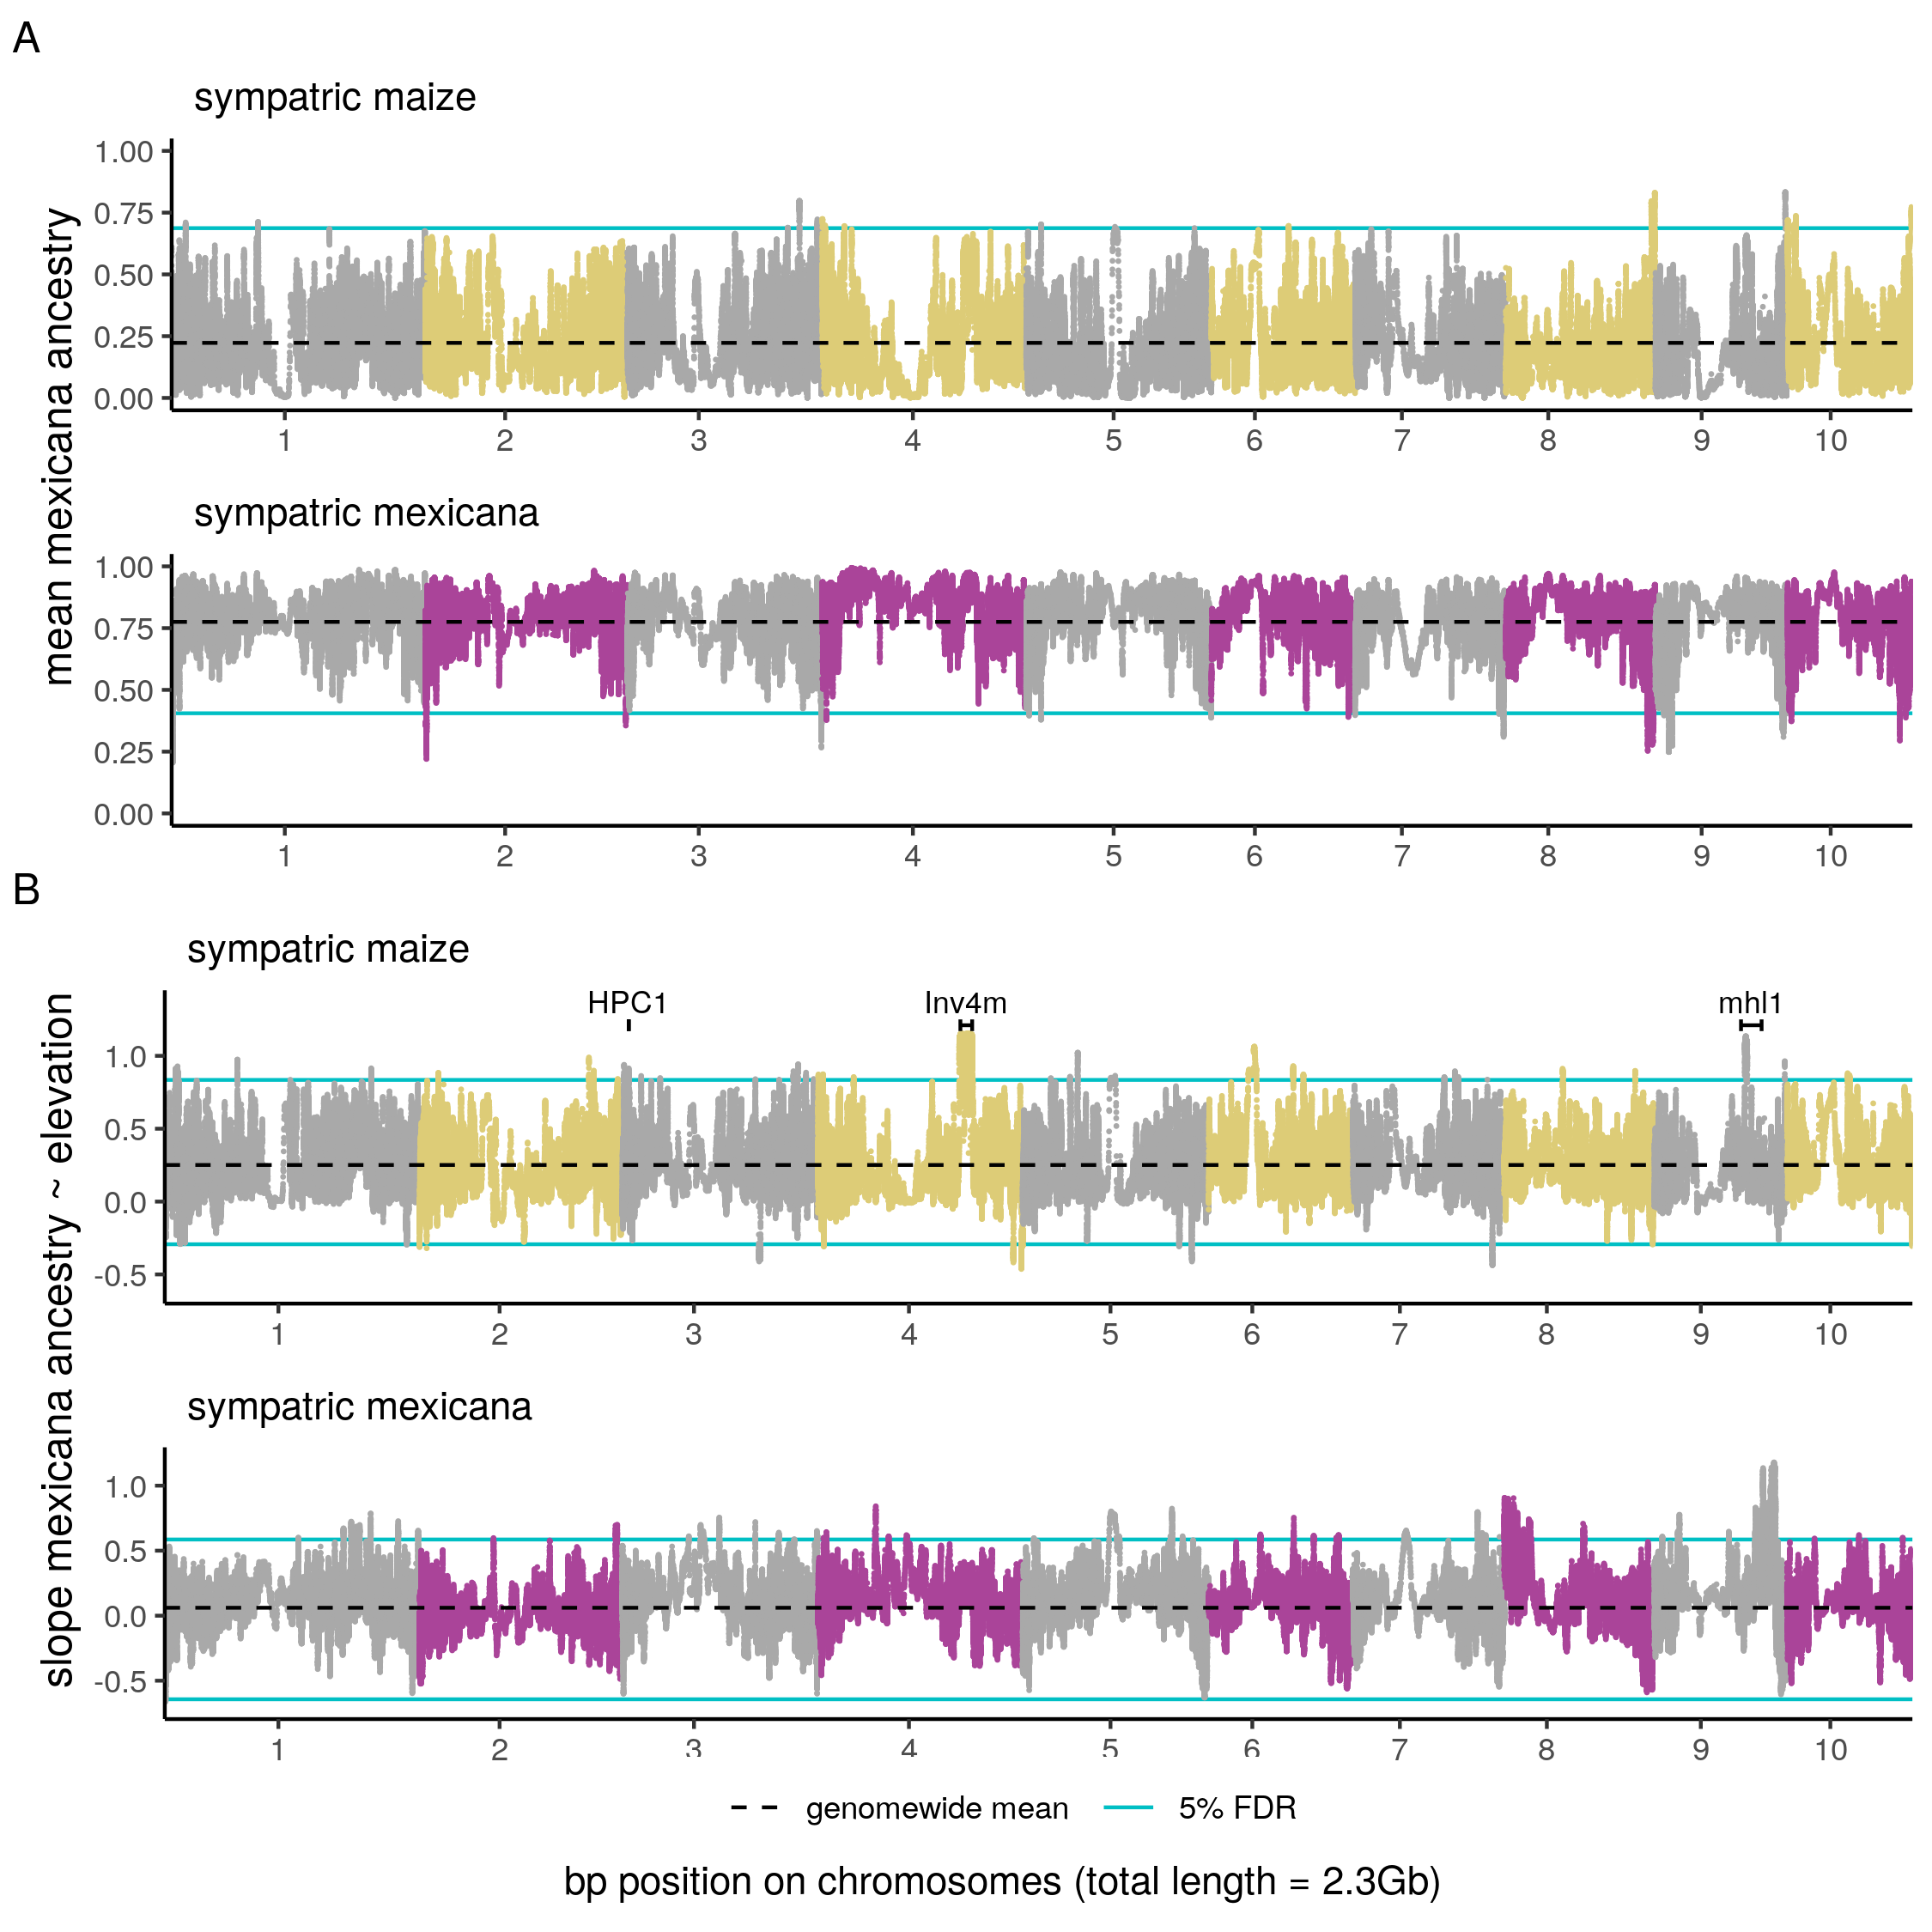
\includegraphics[width=.95\textwidth]{chapter2/figures/multi_maize_mexicana_genome_scan.png}
\caption{\color{Gray} \textbf{Genomewide scan for selection on \textit{mexicana} ancestry}. (A) Mean \mexicana ancestry in sympatric maize  and \mexicana populations. (B) Slope of \mexicana ancestry proportion over a 1 km elevation gain in sympatric maize and \mexicana populations.
In both (A) and (B) the blue lines shows the 5\% false discovery rates, set using multi-variate normal simulations. 
Observing \mexicana ancestry of 0\% in sympatric maize or 100\% in sympatric \mexicana was not unexpected based on simulations.
Positions for \textit{Inv4m} \cite{Pyhajarvi:2013jc} and the \textit{mhl1} locus \cite{Moose_Lauter_Carlson:2004_mhl1} were converted to \ec{the maize reference genome} v4 coordinates using Assembly Converter (ensembl.gramene.org). Chromosome numbers are placed at the centromere midpoint (approximate centromere positions are from \cite{Jiao:2017}).}
\label{genome_scan}
\end{figure}

Additionally, we identify outlier loci across the genome where \mexicana ancestry forms steep clines across elevation (Fig \ref{genome_scan}). 
Our top candidate for strong associations between introgression and elevation in maize is \textit{Inv4m}, a large 14 Mb inversion on chromosome 4 previously identified to have introgressed into high elevation maize landraces \cite{Hufford:2013_crop_wild, Wang:2017, Gonzalez-Segovia:2019, Crow:2020_inv4m}. 
This inversion maintains steep elevational clines within teosintes \cite{Pyhajarvi:2013jc}, overlaps QTLs for leaf pigmentation \cite{Lauter:2004} and macrohairs \cite{Lauter:2004}, and is associated with increased yield in maize at high elevations and decreased yield at low elevations \cite{Crow:2020_inv4m}, but has thus far eluded functional characterization of genes within the inversion \cite{Crow:2020_inv4m}. 


Our second strongest association co-localizes with \textit{macrohairless1} (\textit{mhl1}), a locus on chromosome 9 that controls macrohair initiation on the leaf blade \cite{Moose_Lauter_Carlson:2004_mhl1} and is associated with a major QTL explaining 52\% of macrohair variation between high and low elevation teosinte mapping parents \cite{Lauter:2004}.  
Within teosintes, populations of the lowland ancestor of maize, \textit{parviglumis}, show convergent soft sweeps at the \textit{mhl1} locus not shared by \mexicana \cite{Fustier:2017}. Macrohairs are characteristic highland phenotypes in teosinte and maize and are thought to confer adaptive benefits through insect defence and/or \ec{thermal insulation} \cite{Moya-Raygoza:2016, Lauter:2004}. We identified a 3 Mb outlier region within the larger \textit{mhl1} QTL which we analyzed further using PCA. 
We found three genetic clusters along the first principal component, evidence that an inversion polymorphism (hereafter \textit{Inv9f}) maintains differentiation between maize/\parviglumis and \mexicana haplotypes across this region (Figs \ref{mhl1_slopes}, \ref{mhl1_pca}).
Additionally, principal component two at this inversion separates haplotypes genotyped in maize vs. those genotyped in \mexicana, consistent with the \mexicana allele at this inversion introgressing into maize long enough ago to accumulate maize-specific variation, and subsequently sorting in frequency across contemporary maize populations.

The clinal patterns of admixture that we observe at inversions \textit{Inv4m} and \textit{Inv9f} suggest they contribute to elevation-based adaptation in maize, with variation in their fitness impacts even within the historic elevational range of \mexicana.

While our highest peaks localize
with regions previously associated with characteristic highland phenotypes, many additional outlier regions with steep increases in \mexicana ancestry across elevation have undiscovered associations with local adaptation to elevation. 
Additionally, outliers for steep ancestry slopes across elevation in sympatric \mexicana suggest that introgression from maize into \mexicana may facilitate adaptation in \mexicana to the lower end of its elevational range.

\subsection*{Selection at candidate domestication genes}
We hypothesized that domestication genes will be barriers to introgression bilaterally between maize and \mexicana \cite{Hufford:2013_crop_wild}.
While we do not have power to identify individual outlier genes that have low introgression, we can test for enriched overlap between ‘introgression deserts' and a set of putative domestication genes spread across the genome. 

We examined introgression for a sample of 15 well-characterized domestication genes from the literature (see \nameref{genes_outliers}), and compared them to the regions of the genome with the lowest 5\% introgression genomewide across all sympatric maize or \mexicana populations (‘introgression deserts'). A small but enriched subset of these domestication genes overlap with introgression deserts in sympatric maize (7, P $<$ 0.001) and likewise in sympatric \mexicana (7, P $<$ 0.001).
Among these candidates, we find that \textit{teosinte branched1} (\textit{tb1}), a key transciption factor that regulates branching vs. apical dominance \cite{Doebley_Stec_Gustus:1995_tb1, Doebley_Stec_Hubbard:1997_tb1}, overlaps introgression deserts in both maize and \mexicana, consistent with \textit{tb1}'s role at the top of the domestication regulatory hierarchy \cite{Dong:2019_reg_domestication}.

We also find evidence for reduced introgression into both maize and \mexicana at \textit{teosinte glume architecture1} (\textit{tga1}) \cite{Dorweiler:1993, Wang:2005_tga1} and \textit{brittle endosperm2} (\textit{bt2}) \cite{Whitt:2002_starch}, which are associated with ‘naked' edible grains and starch biosynthesis, respectively. 
Another eight domestication genes \cite{Wills:2018_zagl1, Wills:2013_gt1, Sosso:2015, Vollbrecht:2005_ramosa, Sigmon_Vollbrecht:2010, Lin:2012_shattering, Whitt:2002_starch} have low introgression in one direction only.


Among these, \textit{sugary1} (\textit{su1}) in the starch pathway has low maize ancestry in \mexicana but shows a steep increase in introgressed \mexicana ancestry with elevation in maize ($<$ 5\% FDR), which suggests this gene has pleiotropic effects on non-domestication traits in maize, with fitness trade-offs across elevation. 
\textit{Sugary1} mutations \ec{modify the sweetness, nutrient content and texture of maize kernels (e.g. sweet corn), but} also affect seed germination and emergence at cold temperatures \cite{Trimble:2016_sugary1}, candidate pleiotropic effects that could be more deleterious at higher elevations. 

The remaining four domestication genes do not overlap introgression deserts in either subspecies despite evidence for their role in domestication: \textit{zfl2} (cob rank) \cite{Doebley_Stec:1991, Doebley_Stec:1993, Bomblies_Doebley:2006}, \textit{ba1} (plant architecture) \cite{Gallavotti:2004_ba1}, \textit{ZmSh1-5.1+ZmSh1-5.2} (seed shattering) \cite{Lin:2012_shattering} and \textit{pbf1} (storage protein synthesis) \cite{Wang:1998_pbf}. Despite evidence of introgression at many domestication loci, maize landraces retain all of the classic domestication traits, and \mexicana populations maintain ‘wild' forms. 
Epistasis for domestication traits \cite{Stitzer_Ibarra:2018} could help explain this discrepancy if compensatory effects from other loci contribute to maintaining domestication traits in admixed highland maize, or key domestication alleles segregate at moderate frequencies within \mexicana (but do not have the same phenotypic effects in a teosinte background).

\subsection*{Selection within the flowering time pathway}

Flowering earlier is adaptive in high-elevation environments where days are cooler and there are fewer total growing degree days in a season.
We therefore expect an excess of introgressed \mexicana ancestry at flowering time genes that may contribute to adaptive early flowering in highland maize.
The \mexicana allele at \textit{High PhosphatidylCholine 1} (\textit{HPC1}) has been shown to reduce days to flowering, confers a fitness benefit in maize at higher elevations, and is introgressed in modern flint maize cultivars from Northern Europe and America \cite{Rodriguez-Zapata:2021}. 
Here we show that \textit{HPC1} also overlaps an outlier region with one of the steepest increases in \mexicana ancestry with elevation across sympatric maize populations (+0.91 \mexicana ancestry proportion/km, FDR $<$ 5\%), consistent with a role in adaptive earlier flowering at higher elevations in Mexican landraces. 
\textit{HPC1} has low introgression from maize into sympatric \mexicana across the elevational range of this study, suggesting either that the high-elevation \mexicana allele does not confer fitness tradeoffs in the teosinte background or alternative segregating \mexicana alleles maintain fitness at lower elevations.

We also tested for selection within the flowering time pathway more broadly using a set of 849 candidate flowering time genes \cite{Dong:2012_flowering, Li:2016_flowering}.
Only 1/43 genes from the core flowering time pathway (\textit{ZMM5}) \cite{Dong:2012_flowering} and 15/806 other candidate flowering time genes \cite{Li:2016_flowering} (+/- 20kb) overlap outlier regions with steep increases in \mexicana introgression  with increasing elevation ($<$ 5\% FDR) in sympatric maize, which matches expected overlap by chance ($\sim$2\%,\ P = 0.76).
Thus the steep clinal introgression pattern at \textit{HPC1} in sympatric maize, indicative of strong fitness trade-offs across elevation, is the exception, not the rule, for flowering-time related genes. While for \textit{HPCI} the effect of the \mexicana allele on reducing flowering time has been confirmed by CRISPR \cite{Rodriguez-Zapata:2021}, a limitation for other less-characterized genes is that we simply assume the \mexicana allele reduces flowering time. 
In addition, flowering time is a highly polygenic trait \cite{Buckler:2009}, which could reduce the strength of selection at individual genes with smaller effect sizes than \textit{HPC1} to below what we can detect using steep ancestry clines. 
While it is alternatively possible that \mexicana alleles would show adaptive benefits across the entire range sampled (moderate to high elevation), we find that only 2\ec{/849} candidate flowering time genes overlap high mean \mexicana introgression outliers at a 5\% FDR (P = 0.23).

\section*{Conclusion}
 We conclude that the majority of \mexicana ancestry introgressed into maize over 1000 generations ago and has subsequently been sorted across an elevational gradient, and by selection within individual populations.
 Differentiation of \mexicana haplotypes within maize genomewide ($F_{ST}$) and at individual introgressed outlier loci (e.g. \textit{Inv9f} at the \textit{mhl1} locus (PCA)) corroborate this timeline.
 Despite contemporary observations of \ec{F1} hybrids in the field \cite{Wilkes:1967}, there is little evidence of significant recent gene flow in either direction between sympatric maize-\mexicana population pairs. 
 \ec{Intrinsic genetic incompatibilities and partial temporal isolation (offset flowering times) clearly create an incomplete barrier to gene flow. However, while hybrids are very challenging to identify and weed out from maize fields at early life stages, farmers can easily distinguish between maize and hybrids when choosing which cobs to plant for the next season. In the other direction, hybrids in most locations are expected to be partially temporally isolated from \mexicana and hybrid seeds that do not disarticulate are farmer-dependent for successful dispersal and reproduction, although first-generation backcrosses to \mexicana have been observed \cite{Wilkes:1967}.}

 Consistent with domestication loci acting as barriers to introgression, in both maize and \mexicana an enriched subset of candidate domestication genes overlap ‘introgression deserts.'
 More generally, we find introgressed \mexicana alleles are on average deleterious in maize, but less evidence for a genomewide effect of selection against introgression into \mexicana, possibly because epistasis masks the impact of maize alleles in a \mexicana background \cite{Stitzer_Ibarra:2018}.
 Some loci show exceptional ancestry patterns consistent with selection favoring introgression in multiple populations, especially for \mexicana ancestry in the highest elevation maize. 
 While these shared signatures of adaptive introgression are the most striking, the majority of ancestry peaks are exclusive to a single population.
Despite this signature of geographically-restricted local adaptation from \mexicana ancestry, there is no evidence of local population sources for locally adapted haplotypes at these peaks. Thus both broad and local adaptation of maize throughout the highlands appears to have been driven primarily by the sorting of old introgression.

\section*{Materials and Methods}

\subsection*{Population sampling}
We used maize and \mexicana seed accessions sampled from locations across Mexico in 2008 \cite{Hufford:2013_crop_wild} and currently stored at UC Davis.
We included 14 maize and 14 \mexicana accessions that are paired populations sampled in sympatry from the same locations: Ixtlan*, Amatlan, Penjamillo, Puruandiro*, Nabogame*, El Porvenir*, Santa Clara*, Opopeo*, Xochimilco*, Cocotilan, Tlapala, San Pedro*, Jicaltepec and Tenango del Aire* (see \nameref{population_metadata}). A previous study of crop-wild admixture genotyped different maize and \mexicana individuals from 9 of these locations (marked with *), using the Illumina MaizeSNP50 Genotyping BeadChip \cite{Hufford:2013_crop_wild}. In addition, we chose three population accessions \ec{to sequence as a \mexicana reference panel}: \ec{Puerta Encantada and Malinalco were chosen because they have no record of contemporary maize agriculture nearby and a third population, Amecameca, was added as a complement to these two reference populations because it grows at a higher elevation, beyond the historical range of \parviglumis}.

At each sampling location, multiple ears from maternal plants were collected for seed. 
Population accessions varied in the number of maternal plants with viable seeds. 
When available, we planted multiple seeds within each ear but only randomly selected one individual for sequencing from the plants that successfully germinated in the greenhouse.

\subsection*{DNA extraction and sequencing}
We extracted DNA from leaf tissue and then prepared sequencing DNA libraries using a recently published high-throughput protocol (“Nextera Low Input, Transposase Enabled protocol” \cite{Rowan:2019}) with four main steps: (1) DNA shearing and tagmentation by the Nextera TD enzyme, (2) PCR amplification (Kapa2G Robust PCR kit) and individual sample barcoding (custom 9bp P7 indexing primers) (3) library normalization and pooling, and (4) bead-based clean-up and size-selection of pooled libraries. 
We sequenced the resulting pooled libraries using multiple lanes on Illumina HiSeq 4000 and Novaseq 6000 machines (paired-end 150 bp reads).

To address low sequencing output from some libraries, we re-sequenced 26 libraries (and merged output) and replaced 53 lower-coverage libraries with a higher-coverage library prepared from another seed grown from the same half-sibling family.
We excluded 7 samples from analysis because their final libraries did not yield sufficient sequencing output ($<$0.05x coverage after filtering reads for mapping quality). 
We additionally removed one lane of sequencing (58 samples) from the study after determining a labelling error had occurred for that plate. 

In total, we obtained whole genome sequences for 348 individuals (1.0x average coverage, range: 0.1-2.4x). 
Of these samples, 43 are \mexicana from three allopatric populations, with a total of 34.1x combined coverage. 
The remaining samples are maize and \mexicana from sympatric populations, 262 of which have sufficient coverage for local ancestry inference ($\geq$ 0.5x, 6-12 per sympatric population, see Fig \ref{sequenced_ind_counts}). 
Raw sequencing reads for these low-coverage maize and \mexicana genomes are available at NCBI (PRJNA657016).

\subsection*{Reference genome and recombination map}
We used version 4 of the B73 maize reference genome \cite{Jiao:2017} (Zea\_mays.B73\_RefGen\_v4.dna.toplevel.fa.gz, downloaded 12.18.2018 from Gramene). 
% URL would be better

To find local recombination rates, we converted marker coordinates from a published 0.2 cM genetic map \cite{Ogut:2015df} to the v4 maize genome using Assembly Converter (ensembl.gramene.org). 
We removed any markers that mapped to a different chromosome or out of order on the new assembly, and extended the recombination rate estimates for the most distal mapped windows to the ends of each chromosome. % (Fig \ref{linkage_map})
From this map, we used \textit{approx()} in R (v3.6.2 \cite{R_stats}) to estimate the cM position for any bp position, based on linear interpolation.

\subsection*{Read mapping and filtering}
First, we checked read quality using fastQ Screen (v0.14.0 \cite{Wingett:2018_fastqscreen}) and trimmed out adapter content from raw sequencing reads using the trimmomatic wrapper for snakemake (0.59.1/bio/trimmomatric/pe) \cite{Bolger:2014_trimmomatic}.
We mapped trimmed reads to the maize reference genome using bwa mem (v0.7.17 \cite{Li:2013_bwa}). 
We then sorted reads using SAMtools (v1.9 \cite{Li:2009samtools}), removed duplicates using picardtools (v2.7.1) MarkDuplicates and merged libraries of the same individual sequenced on multiple lanes using SAMtools merge. 
In all subsequent analyses in the methods below we filtered out reads with low mapping scores ($<$ 30) and bases with low base quality scores ($<$ 20).

\subsection*{High-coverage \textit{Tripsacum} genome sequencing}
In addition to low-coverage genomes for maize and \mexicana, we selected a \textit{Tripsacum dactyloides} individual as an outgroup and sequenced it to high coverage. This individual is an outbred ‘Pete' cultivar (rootstock acquired from the Tallgrass Prairie Center, Iowa, USA). We extracted genomic DNA from leaf tissue using the E.Z.N.A.® Plant DNA Kit (Omega Biotek), following manufacturer’s instructions, and then quantified DNA using Qubit (Life Technologies). We prepared a PCR-free Truseq DNA library and sequenced it with an Illumina HiSeq2500 rapid run (paired-end 250 bp reads). We generated a total of 136.53 Gb of sequencing for this individual, available at NCBI (SRR7758238). 
For the following analyses that use \textit{Tripsacum} as an outgroup, we randomly subsampled 50\% of reads using seqtk, for approximately 30x coverage. We mapped reads to the maize reference using the pipeline described above, and additionally capped base quality scores with the ‘extended BAQ' model in SAMtools \cite{Li:2011_BAQ}, which reduces the influence of bases with lower alignment quality.

\subsection*{Additional genomes from published sources}
For an allopatric maize reference population, we used 55 previously published high-coverage maize genomes from \ec{a Tuxpe{\~n}o landrace grown near} Palmar Chico (NCBI: PRJNA616247 \ec{\cite{Chen:2020_maize55, Yang:2019}}). This \ec{maize} population grows \ec{at 983 m}, below the elevational range for \mexicana. 

For a parviglumis reference population, we used 50 previously published high-coverage lowland individuals sampled from the ‘Mound' population at 1,008 m \ec{near} Palmar Chico  \cite{vanHeerwaarden:2010, Yang:2019, Chen:2020_maize55} (NCBI: PRJNA616247, see \nameref{parv50}). We mapped and filtered reads for these individuals using the pipeline described above and capped base quality scores using BAQ.


\subsection*{SNP calling}
We called SNPs using a combined panel of the 348 low-coverage genomes sequenced in this study for sympatric maize, sympatric \mexicana, and allopatric \mexicana, and the 55 high-coverage allopatric maize reference genomes described above. We used ANGSD (v0.932 \cite{Korneliussen:2014_ANGSD}) to identify variant sites with minor allele frequencies $\geq$ 5\% in the total sample based on read counts (‘angsd -doMajorMinor 2 -minMaf 0.05 -doCounts 1 -doMaf 8'). In addition to mapping and base quality filters (‘-minMapQ 30 -minQ 20'), we capped base qualities using the extended per-Base Alignment Quality algorithm (‘-baq 2' \cite{Li:2011_BAQ}) and removed sites that did not have at least 150 individuals with data or had sequencing depth exceeding 2.5x the total sample mean depth. To apply this total depth filter, we estimated mean depth (‘angsd -doCounts 1 -doDepth 1 -maxDepth 10000') for 1000 regions of length 100bp randomly sampled using bedtools (v2.29.0 \cite{Quinlan:2010_bedtools}). 
In total, we identified 52,118,357 SNPs on the assembled chromosomes. In conjunction with SNP calling, we produced genotype likelihoods for each individual at these variant sites using the SAMtools GL method \cite{Li:2009samtools} implemented in ANGSD (‘-GL 1 -doGlf 2').

\subsection*{Global ancestry inference}
To estimate genetic relationships between populations and their genomewide ancestry proportions, we used methods specific to low-coverage data that rely on genotype likelihoods, rather than called genotypes. 
Because these methods are sensitive to SNPs in high linkage disequilibrium (LD), we thinned genotype likelihoods to every 100th SNP ($\sim$4kb spacing) \cite{Tenaillon:2001_LD}.
To confirm that maize and \mexicana subspecies form a major axis of genetic variation in our sample, we estimated the genetic covariance matrix between individuals using PCAngsd (v0.98.2 \cite{Meisner:2018_pcangsd}) and visualized principal components computed using \textit{eigen()} in R. 
We then estimated global ancestry proportions using the same thinned genotype likelihood files as input to NGSAdmix \cite{Skotte:2013_NGSadmix},  using K = 2 clusters. 
Clusters clearly mapped onto the two reference groups, which we used to label the two ancestry components as ‘maize' and ‘\mexicana'.

\subsection*{Local ancestry and timing of admixture}
We inferred local ancestry across the genome using a hidden Markov model that is appropriate for low-coverage data because it models genotype uncertainty down to the level of read counts for all admixed individuals (ancestry\_hmm \cite{CorbettDetig:2017gh}). 
This method relies on allele counts from separate reference populations to estimate allele frequencies for each ancestry. 
Because some of our reference individuals have too low of coverage to accurately call genotypes, we randomly sampled one read per individual to get unbiased frequency estimates for major and minor alleles at each site (‘angsd -doCounts 1 -dumpCounts 3'). 
To maximize ancestry-informativeness of sites in this analysis, we identified SNPs with allele frequency differences of at least 0.3 between subspecies (‘angsd -doMajorMinor 3 -GL 1 -baq 2 -doMaf 1') estimated from at least 44 reference maize and 12 reference \mexicana individuals with sequencing coverage at a site.
We then calculated genetic distances between SNPs \ec{using the maize recombination map} and filtered our enriched variants to \ec{have minimum 0.001 cM spacing between adjacent SNPs} . 

Running ancestry\_hmm jointly infers local ancestry for each individual and the time since admixture. \ec{This HMM method assumes a neutral demographic history in which a constant-size admixed population was formed by a single admixture event $t$ generations in the past, and finds the $t$ that maximize the likelihood of the observed read counts and hidden local ancestry state across each admixed individual's genome. The timing of admixture defines the generations for possible meiotic recombination between ancestry tracts, and therefore scales the transition probabilities between hidden ancestry states. In addition to $t$, the HMM outputs the posterior probabilities for homozygous maize, homozygous \mexicana, and heterozygous ancestry for each individual at every site.} 
\ec{We analysed each} sympatric maize \ec{and} \mexicana population separately, using the population's mean NGSAdmix global ancestry estimate as a prior for mixing proportions, 100 generations as a prior for admixture time (range: 0-10000), an approximate effective population size (Ne) of 10,000 individuals, \ec{genetic positions for each SNP based on the maize linkage map,} and an estimated sequencing base error rate of $3\times10^{-3}$. 
We ran ancestry\_hmm with an optional setting to bootstrap 100 random samples of 1,000-SNP genomic blocks to estimate uncertainty around the estimated generations since admixture \ec{($t$)}. To test the sensitivity of the HMM to our choice of Ne, we re-ran ancestry\_hmm with two other Ne's that differ by an order of magnitude (Ne = 1k, 100k), but did not analyze these results further after finding high correspondence for both local ancestry and timing estimates. 

To get a single point estimate for local ancestry at a site for an individual, \ec{we computed a sum of \mexicana ancestry from the different possible ancestry states, weighted by their posterior probabilities}: \mexicana ancestry proportion = P(homozygous \mexicana) + $\nicefrac{1}{2}$P(heterozygous \ec{maize-\mexicana}). 
In addition, for analyses that require ancestry tract positions, we assumed that the estimated ancestry at a focal site extends halfway to the next site with a local ancestry estimate. 

\subsection*{Diversity within ancestry}
Using \mexicana ancestry estimates from the HMM, we identified high-confidence homozygous ancestry tracts for both maize and \mexicana ancestry (posterior $>$ 0.8). 
We filtered individual bams for reads that overlap these tracks and used the resulting filtered bams to calculate diversity within both maize and 
\mexicana ancestry, separately. 
We estimate diversity using the ANGSD/realSFS framework which is appropriate for low-coverage sequence data it takes into account uncertainty in both genotypes and variant sites. 
We created a concensus fasta sequence for \textit{Tripsacum} (‘angsd -doFasta 2') to use as the ancestral state \ec{for polarizing the unfolded site frequency spectrum in} these analyses.

For each population and ancestry, we estimated the site allele frequencies (‘angsd -doSaf 1 -GL 1') and subsequently estimated the genomewide site frequency spectrum (SFS). We then used this SFS as a prior to estimate within-ancestry pairwise diversity ($\pi$) genomewide from the site allele frequencies (‘realSFS saf2theta'). 

For each pair of populations and ancestry, we additionally used realSFS to estimate the two dimensional SFS from the individual population site allele frequencies genomewide. We then used this 2D SFS as a prior to estimate genomewide within-ancestry $F_{ST}$ between the two populations (‘realSFS fst index -whichFst 1'). 
This call uses Hudson's $F_{ST}$ estimator \cite{Hudson:1992_fst} as parameterized in \cite{Bhatia:2013_fst}.

\subsection*{Effect of local recombination rate on introgressed ancestry}
To estimate the effects of linked selection and recombination rate on genomewide introgression patterns, we compared \mexicana ancestry estimates across genomic quintiles. 
Based on a 0.2 cM-resolution recombination map \cite{Ogut:2015df} for maize, we merged adjacent recombination windows into larger 1 cM non-overlapping windows and calculated each window's mean recombination rate and overlap with coding base pairs (bedr ‘coverage') \cite{R_bedr}. 
We retrieved coding regions (‘CDS') using gene annotations from Ensembl (ensemblgenomes.org, Zea\_mays.B73\_RefGen\_v4.41.chr.gff3.gz, dowloaded 11.6.2018). 
We sorted windows into quintiles for either recombination rate or coding density (bp/cM). 
Each quintile covers approximately $\nicefrac{1}{5}$ of the genome based on physical bp.

\subsection*{i. NGSAdmix estimates}
To estimate ancestry proportions for each recombination rate quintile, we first reduced LD by thinning to 1\% of SNPs (every 100th) and ran NGSAdmix 5 times separately (once per quintile) with K=2 clusters. 
We assigned  ‘maize' and ‘\textit{mexicana}' labels to the ancestry clusters based on majority assignment to the respective allopatric reference panels. 
To bootstrap for uncertainty, we re-sampled 1 cM windows with replacement from each quintile 100 times, and re-ran NGSAdmix on the resulting bootstrap SNP sets. 
Using these results, we calculated 95\% percentile bootstrap confidence intervals for the estimated admixture proportions, and the Spearman's rank correlation between the recombination rate (or coding bp per cM) and admixture proportion ranks for each quintile. 
We also tested for a difference in ancestry slopes with elevation across different recombination rate quintiles by fitting a linear model with an elevation by recombination quintile interaction term: \mexicana ancestry $\sim$ elevation + r + elevation*r. 
Using lm() in R, we fit this model for sympatric maize and sympatric \mexicana separately, treating quintiles as a numeric scale 0-4.

\subsection*{$f_4$ estimates}
In a complementary analysis, we used a ratio of $f_4$ statistics as an alternative method to estimate ancestry proportions by quintile.  \ec{The $f_4$ statistic measures shared genetic drift (allelic covariance) between populations in a phylogeny, due to either shared branch lengths or admixture events in the evolutionary history relating these populations.} 
%and up to a scaling factor is equivalent to the ABBA-BABA statistic. 
\ec{Excess shared drift with one population from a pair of sister populations in the tree is a signature of admixture, analogous to the ABBA-BABA test \cite{Green:2010}, and a ratio of two $f_4$ statistics can be used to quantify the admixture proportion.} 
Assuming the basic phylogenetic tree (((\parviglumis, allopatric maize), allopatric \mexicana), \textit{Tripsacum}) in Fig \ref{f4_tree}, we can estimate $\alpha$, the proportion of ancestry inherited from \mexicana in an admixed population, as follows \cite{Green:2010, Peter:2016}:
$$ \alpha = \frac{f_4(\text{Tripsacum, \parviglumis; X, allopatric maize})}{f_4(\text{Tripsacum, \parviglumis; allopatric \mexicana, allopatric maize)}}.$$
The denominator of this statistic estimates the branch length leading to \parviglumis and allopatric maize that separates these sister subspecies from allopatric \mexicana; the full ratio estimates the proportion of this branch that separates sympatric population X from \parviglumis and allopatric maize, i.e. the \mexicana ancestry in X. 
Because the $f_4$ statistic is sensitive to additional unmodeled admixture within the tree, we limited our allopatric \mexicana group to individuals from just one of the three reference populations (Amecameca), which showed no evidence of admixture in our global ancestry analysis (see Fig \ref{global_anc_multi}).

For each 1 cM window across the genome, we used ANGSD to calculate ABBA-BABA statistics from observed read counts for the 4 populations in the numerator and denominator of the $\alpha$ estimator separately (‘angsd -doabbababa2 1 -remove\_bads 1 -minMapQ 30 -minQ 20 -doCounts 1 -doDepth 1 -maxDepth 10000 -useLast 1 -blockSize 5000000').
From the resulting output files, we summed the negative of the ABBA-BABA numerator (‘Num') and divided by the total number of included sites (‘nSites') across all 1 cM windows within a quintile to get the $f_4$ statistic \cite{Soraggi:2018}. 

We then calculated the Spearman's rank correlation between the recombination rate quintiles and admixture proportion ranks for these quintiles. 
We calculated simple bootstrap confidence intervals for our ancestry estimates and correlations by re-sampling 1 cM windows within quintiles with replacement 10,000 times and re-calculating the $f_4$ ratios and resulting rank correlation across quintiles to construct 95\% percentile confidence intervals. 
We repeated this analysis using quintiles based on coding bp per cM in place of recombination rate (cM/Mbp).

\subsection*{ii. Local ancestry estimates}
We also calculated the Spearman's rank correlation between local recombination rate (or coding bp per cM) and local ancestry proportion at the level of individual 1 cM windows. 
For each window, we averaged local ancestry estimates from the HMM across all individuals within sympatric maize, and separately, sympatric \mexicana. 
We then calculated simple bootstrap confidence intervals for our local ancestry estimates and local recombination rate (or coding bp per cM) by re-sampling 1 cM windows across the genome with replacement 10,000 times and re-calculating the rank correlation across windows to construct 95\% percentile confidence intervals.


\subsection*{Local ancestry simulations}

%Here, the demographic history (and therefore independence) of admixed populations was previously unknown because of %potential long-distance (and in the case of maize, likely human-facilitated) gene flow between populations.

We simulated \mexicana ancestry population frequencies using a multivariate-normal null model:

$$mexicana\ \text{ancestry} \sim \text{MVN}(\vec{\alpha}, K)$$
where $\vec{\alpha}$ is the vector of mean \mexicana ancestry frequencies genomewide for each sympatric population and $K$ is the empirical ancestry variance-covariance matrix relating these 14 populations. 
The diagonal entries of the K matrix capture the expected variation in local ancestry across the genome within populations due to drift and random sampling. 
The off-diagonals capture ancestry covariances between populations created by shared gene flow and drift post-admixture: at loci where one population has an excess of introgression, other admixed populations with shared demographic history will also tend to have an excess of introgression.

To construct K, we calculated the covariance in ancestry between each pair of populations \textit{i} and \textit{j}  using all \textit{L} loci with local ancestry calls genomewide:

\begin{align*}
K[i, j] = \frac{1}{L} \sum_{l=1}^{L} (Anc_{i,l} - \alpha_i)(Anc_{j,l} - \alpha_j).
\end{align*}

Above, $Anc_{i,l}$ and $Anc_{j,l}$ are local ancestry frequencies at a locus \textit{l} while $\alpha_i$ and $\alpha_j$ are the mean local ancestry frequencies across the genome for populations \textit{i} and \textit{j}.

For sympatric maize and sympatric \mexicana separately, we calculated the empirical K matrix between populations from all 14 sympatric locations, and then took 100,000 independent draws from their MVN distribution, thereby simulating \mexicana ancestry for all populations at 100,000 unlinked loci. 
Because ancestry frequencies are bounded at [0,1] but normal distributions are not, we truncated any simulated values outside of this range.

\subsection*{Introgression peaks shared between populations}
To characterize introgression peak sharing between individual populations, we defined ‘ancestry peaks' as sites where a population has over 2 standard deviations more introgressed ancestry than the genomewide mean. 
We counted the number of peaks that are shared between all pairs and combinations of populations. 
To compare these results to our null model, we also counted the number of introgression peaks shared by populations in our simulated dataset, using the 2 s.d. cutoff set by the empirical data to define peaks.

Because \mexicana ancestry shows significant diversity, we additionally characterized diversity for \mexicana ancestry peaks introgressed into maize. 
For all introgressed ancestry outlier regions in a focal maize population, we used ANGSD to estimate pairwise diversity within the population ($\pi$) and differentiation ($F_{ST}$) between the focal sympatric maize populations and their local sympatric \mexicana population.
We focused on the \mexicana ancestry within peaks by limiting our diversity estimates to only include high-confidence homozygous \mexicana ancestry tracts (posterior $>$ 0.8). 
For these analyses, we pooled information across outlier peaks, but distinguish between introgression peaks exclusive to the focal population and introgression peaks shared between the focal population and at least 3 other sympatric maize populations.
We used global estimates of the SFS and 2D SFS as priors to estimate $\pi$ and $F_{ST}$ for the subsets of the genome within introgression peaks, and otherwise followed the same methods listed above in ‘Diversity within ancestry'. 

\subsection*{Genomewide scan for ancestry outliers}

For sympatric maize and \mexicana separately, we calculated the mean \mexicana ancestry across all individuals at a locus, and fit a linear model using lm() in R to estimate the slope of \mexicana ancestry frequencies for sympatric populations across elevation (km): \mexicana ancestry $\sim$ elevation. We then repeated these summary statistics for every locus with an ancestry call in the empirical data and each simulated locus in the MVN simulated data.

We calculated 5\% false-discovery-rate (FDR) cutoffs for high and low \mexicana ancestry using the Benjamini-Hochberg method \cite{Benjamini_Hochberg:1995} and simulation results to estimate the expected frequency of false-positives under our null MVN model (one-tailed tests). 
We repeated this approach to identify outlier loci with steep positive (or negative) slopes for \mexicana ancestry across elevation at a 5\% FDR. 

\subsection*{Test for reduced introgression at domestication genes}
%\subsection*{Test for reduced introgression at domestication loci}
%We used the 31 landraces from Wang \cite{Wang:2017} to identify selective sweep patterns indicative of loci involved in the domestication of maize. 
%Specifically, we mapped reads from each accession to the maize v4 reference and called variants using the GATK germline variant call best practices to call SNPs from the alignments. We then used RAiSD to characterize sweeps from these genotypes.
%RAiSD was run under default settings and the only modification we made was to use the script mop (https://github.com/RILAB/mop) to quantify unmappable reads for each RAisD window and adjusted the window size in the RAiSD output to reflect the mappable bases, as opposed to the physical number of bases in each window.

To test whether domestication genes are unusually resistant to introgression, we first defined ‘introgression deserts' as regions with the lowest 5\% of introgression genomewide across all sympatric maize (or, separately, sympatric \mexicana) populations. We then looked up v4 coordinates on Ensembl.org for genes associated with maize domestication in the literature (\nameref{genes_outliers}), and used bedtools ‘intersect' to identify which of these genes $\pm 20$ kb overlap introgression deserts. To test for significance, we randomly shuffled the gene positions across the genome (bedtools ‘shuffle') 1000 times and re-calculated overlap with introgression deserts for each permuted data set.

\subsection*{Test for selection within the flowering time pathway}
We identified a list of 48 core flowering time pathway genes from the literature \cite{Dong:2012_flowering}, and a broader list of 905 flowering time candidate genes \cite{Li:2016_flowering, Dong:2012_flowering}. 
From the combined set, we included 849 total genes (43 core pathway) which we were able to localize on assembled autosomes of the v4 reference genome using MaizeGDB gene cross-reference files \cite{Portwood:2019_MaizeGDB}.
We counted the number of genes $\pm 20$ kb that intersected with outlier regions for steep increases in \mexicana introgression with elevation (and, separately, high \mexicana introgression) in sympatric maize populations ($<$ 5\% FDR) using bedtools ‘intersect', then tested for significance by repeating this analysis with 1000 randomly shuffled gene positions.


\subsection*{Analysis pipeline and data visualization}

We constructed and ran bioinformatics pipelines using snakemake (v.5.17.0 \cite{Koester_Rahmann:2012_snakemake}) within a python conda environment (v3.6). 
We analyzed and visualized data in R (v3.6.2 \cite{R_stats}) using the following major packages: tidyverse (v1.3.0 \cite{R_tidyverse}), viridis (v0.5.1 \cite{R_viridis}), bedr (v1.0.7 \cite{R_bedr}), boot (v.1.3\_25 \cite{R_boot, Davison_Hinkley:1997_boot}), gridExtra (v2.3 \cite{R_gridExtra}), ggupset (v0.3.0 \cite{R_ggupset}) and tidygraph (1.2.0 \cite{R_tidygraph}). 
All scripts can be found on our gitHub repository, https://github.com/ecalfee/hilo, which also includes a full list of software and versions (see envs/environment.yaml).


\section*{Acknowledgments}
The authors would like to acknowledge funding from NSF award number 1546719 to JRI and GC. This work was also supported by the National Institute of General Medical Sciences of the National Institutes of Health (NIH R01 GM108779 and R35 GM136290, awarded to GC). We thank Pesach Lubinsky for collecting the seeds sequenced in this study. We also want to thank the Coop and Ross-Ibarra labs, and the HILO and Zeavolution working groups for helpful feedback on this work.


\medskip

\section*{Associated Publication}
An earlier version of Chapter 2 was posted as a preprint to BioRxiv on March 5, 2021. This preprint will be updated with a link to the final peer-reviewed article upon publication: \newline

Calfee E, Gates D, Lorant A, Perkins TA, Coop G, Ross-Ibarra J. Selective sorting of ancestral introgression in maize and teosinte along an elevational cline. BioRxiv. 2021;\\
doi:10.1101/2021.03.05.434040

%This is where your bibliography is generated. Make sure that your .bib file is actually called library.bib
%\bibliography{chapter2/library}


%This defines the bibliographies style. Search online for a list of available styles.
%\bibliographystyle{plos2015}

\newpage
\section*{Supporting Information}

%\newpage

\paragraph*{Table 2.1}
\label{population_metadata}
{\bf Population metadata.} 
\begin{table}[ht]
\centering
\begin{tabular}{llllllll}
\hline
Subspecies & Group & Location & Country & \makecell[lt]{Elev.\\ (m)} & Latitude & Longitude & Accession \\
\hline
\mexicana & allopatric & \makecell[lt]{Puerta\\ Encantada} & Mexico & 1658 & 18.9725 & -99.0298 & RIMME0033 \\
\mexicana & allopatric & Malinalco & Mexico & 1887 & 18.9531 & -99.503 & RIMME0020 \\
\mexicana & allopatric & Amecameca & Mexico & 2467 & 19.139 & -98.7733 & RIMME0022 \\
maize & sympatric & Ixtlan & Mexico & 1547 & 20.1683 & -102.373 & RIMMA0371 \\
maize & sympatric & Amatlan & Mexico & 1658 & 18.9719 & -99.0551 & RIMMA0369 \\
maize & sympatric & Penjamillo & Mexico & 1705 & 20.1176 & -101.93 & RIMMA0361 \\
maize & sympatric & Puruandiro & Mexico & 1915 & 20.1076 & -101.49 & RIMMA0370 \\
maize & sympatric & Nabogame & Mexico & 2020 & 26.2465 & -106.915 & RIMMA0360 \\
maize & sympatric & El Porvenir & Mexico & 2094 & 19.6789 & -100.64 & RIMMA0363 \\
maize & sympatric & Santa Clara & Mexico & 2173 & 19.4184 & -101.642 & RIMMA0362 \\
maize & sympatric & Opopeo & Mexico & 2213 & 19.4181 & -101.613 & RIMMA0368 \\
maize & sympatric & Xochimilco & Mexico & 2237 & 19.2861 & -99.0827 & RIMMA0374 \\
maize & sympatric & Cocotilan & Mexico & 2269 & 19.2244 & -98.8427 & RIMMA0367 \\
maize & sympatric & Tlapala & Mexico & 2272 & 19.2351 & -98.8368 & RIMMA0365 \\
maize & sympatric & San Pedro & Mexico & 2459 & 19.0886 & -98.4935 & RIMMA0372 \\
maize & sympatric & Jicaltepec & Mexico & 2587 & 19.3764 & -99.6303 & RIMMA0366 \\
maize & sympatric & \makecell[lt]{Tenango\\ del Aire} & Mexico & 2609 & 19.1197 & -99.5896 & RIMMA0373 \\
\mexicana & sympatric & Ixtlan & Mexico & 1547 & 20.1683 & -102.373 & RIMME0029 \\
\mexicana & sympatric & Amatlan & Mexico & 1658 & 18.9719 & -99.0551 & RIMME0027 \\
\mexicana & sympatric & Penjamillo & Mexico & 1705 & 20.1176 & -101.93 & RIMME0019 \\
\mexicana & sympatric & Puruandiro & Mexico & 1915 & 20.1076 & -101.49 & RIMME0028 \\
\mexicana & sympatric & Nabogame & Mexico & 2020 & 26.2465 & -106.915 & RIMME0018 \\
\mexicana & sympatric & El Porvenir & Mexico & 2094 & 19.6789 & -100.64 & RIMME0021 \\
\mexicana & sympatric & Santa Clara & Mexico & 2173 & 19.4184 & -101.642 & RIMME0034 \\
\mexicana & sympatric & Opopeo & Mexico & 2213 & 19.4181 & -101.613 & RIMME0026 \\
\mexicana & sympatric & Xochimilco & Mexico & 2237 & 19.2861 & -99.0827 & RIMME0035 \\
\mexicana & sympatric & Cocotilan & Mexico & 2269 & 19.2244 & -98.8427 & RIMME0025 \\
\mexicana & sympatric & Tlapala & Mexico & 2272 & 19.2351 & -98.8368 & RIMME0023 \\
\mexicana & sympatric & San Pedro & Mexico & 2459 & 19.0886 & -98.4935 & RIMME0030 \\
\mexicana & sympatric & Jicaltepec & Mexico & 2587 & 19.3764 & -99.6303 & RIMME0024 \\
\mexicana & sympatric & \makecell[lt]{Tenango\\ del Aire} & Mexico & 2609 & 19.1197 & -99.5896 & RIMME0031 \\
\hline 
\end{tabular} 
\end{table}

\newpage

\paragraph*{Table 2.2}
\label{parv50}
{\bf Parviglumis SRA IDs.} 
\begin{table}[ht]
\centering
\begin{tabular}{llll}
\hline
Run & Isolate & Run (cont.) & Isolate (cont.) \\
\hline
SRR11448802 & PC\_M59\_ID1 & SRR13207117 & PC\_J01\_ID1 \\
SRR11448838 & PC\_I05\_ID1 & SRR11448791 & PC\_N48\_ID1 \\
SRR11448793 & PC\_N13\_ID1 & SRR11448812 & PC\_L08\_ID1 \\
SRR11448797 & PC\_N09\_ID1 & SRR11448834 & PC\_I50\_ID1 \\
SRR11448799 & PC\_N07\_ID1 & SRR13207120 & PC\_O08\_ID1 \\
SRR11448800 & PC\_N04\_ID1 & SRR11448794 & PC\_N11\_ID1 \\
SRR11448803 & PC\_M58\_ID1 & SRR11448804 & PC\_M15\_ID1 \\
SRR11448805 & PC\_M05\_ID1 & SRR11448807 & PC\_L56\_ID1 \\
SRR11448809 & PC\_L14\_ID1 & SRR13207095 & PC\_J08\_ID1 \\
SRR11448811 & PC\_L12\_ID1 & SRR13207116 & PC\_O59\_ID1 \\
SRR11448814 & PC\_K60\_ID1 \\
SRR11448816 & PC\_K54\_ID1 \\
SRR11448818 & PC\_K02\_ID1 \\
SRR11448819 & PC\_J51\_ID1 \\
SRR11448820 & PC\_J50\_ID1 \\
SRR11448823 & PC\_J13\_ID1 \\
SRR11448824 & PC\_J12\_ID1 \\
SRR11448825 & PC\_J10\_ID1 \\
SRR11448827 & PC\_J04\_ID1 \\
SRR11448830 & PC\_I58\_ID1 \\
SRR11448832 & PC\_I52\_ID1 \\
SRR11448836 & PC\_I08\_ID1 \\
SRR11448837 & PC\_I06\_ID1 \\
SRR13207106 & PC\_J07\_ID1 \\
SRR13207118 & PC\_O51\_ID1 \\
SRR13207119 & PC\_O10\_ID1 \\
SRR13207121 & PC\_N60\_ID1 \\
SRR13207122 & PC\_N58\_ID1 \\
SRR13207123 & PC\_N57\_ID1 \\
SRR13207124 & PC\_N56\_ID1 \\
SRR13207125 & PC\_N14\_ID1 \\
SRR13207126 & PC\_N10\_ID1 \\
SRR13207127 & PC\_L48\_ID1 \\
SRR13207128 & PC\_I53\_ID1 \\
SRR13207129 & PC\_I11\_ID1 \\
SRR13207130 & PC\_L10\_ID1 \\
SRR13207131 & PC\_L06\_ID1 \\
SRR13207138 & PC\_K55\_ID1 \\
SRR13207149 & PC\_J48\_ID1 \\
SRR13207160 & PC\_J14\_ID1 \\
% \\
% \\
% \\
% \\
% \\
% \\
% \\
% \\
% \\
% \\
\hline 
\end{tabular} 
\end{table}


\newpage

\paragraph*{Table 2.3}
\label{spearmans_rho_ngsadmix}
{\bf Spearman's rank correlation between \mexicana ancestry (NGSAdmix) and recombination rate (or coding bp per cM) quintiles}
% latex table generated in R 3.6.2 by xtable 1.8-4 package
% Thu Feb  4 23:14:59 2021
\begin{table}[ht]
\centering
\begin{tabular}{llrrr}
  \hline
group & feature & Spearman's $\rho$ & 2.5\% & 97.5\% \\ 
  \hline
allopatric maize & recombination rate (cM/Mb) & -0.36 & -0.90 & 0.67 \\ 
  allopatric mexicana & recombination rate (cM/Mb) & 0.40 & 0.10 & 1.00 \\ 
  sympatric maize & recombination rate (cM/Mb) & 1.00 & 0.85 & 1.00 \\ 
  sympatric mexicana & recombination rate (cM/Mb) & 1.00 & 0.90 & 1.00 \\ 
  allopatric maize & coding bp per cM & 0.62 & -0.30 & 1.00 \\ 
  allopatric mexicana & coding bp per cM & -0.40 & -0.90 & -0.20 \\ 
  sympatric maize & coding bp per cM & -1.00 & -1.00 & -0.85 \\ 
  sympatric mexicana & coding bp per cM & -0.90 & -1.00 & -0.80 \\ 
   \hline
\end{tabular}
\end{table}


\paragraph*{Table 2.4}
\label{spearmans_rho_f4_sympatric_maize_pop22}
{\bf Spearman's rank correlation between ancestry ($f_4$ ratio) and recombination rate (or coding bp per cM) quintiles in sympatric maize}
% latex table generated in R 3.6.2 by xtable 1.8-4 package
% Thu Feb  4 23:22:58 2021
\begin{table}[ht]
\centering
\begin{tabular}{llrrr}
  \hline
group & feature & Spearman's $\rho$ & 2.5\% & 97.5\% \\ 
  \hline
sympatric maize & recombination rate (cM/Mb) & 1.00 & 0.30 & 1.00 \\ 
  sympatric maize & coding bp per cM & -0.90 & -1.00 & 0.10 \\ 
   \hline
\end{tabular}
\end{table}


\paragraph*{Table 2.5}
\label{tbl_elev_r_interaction_5}
{\bf Ancestry by elevation and recombination rate quintile.} Best-fitting linear models for ancestry proportion predicted by an elevation by recombination rate interaction: \mexicana ancestry $\sim$ elevation + r + elevation*r. Here, r is the recombination rate quintile, treated as numeric [0-4]. This model only uses ancestry estimates for sympatric individuals and is fit separately for maize and \mexicana samples.
% latex table generated in R 3.6.2 by xtable 1.8-4 package
% Thu Feb  4 23:14:59 2021
\begin{table}[ht]
\centering
\begin{tabular}{llrrrr}
  \hline
group & term & estimate & std.error & statistic & p.value \\ 
  \hline
sympatric maize & intercept & -0.122 & 0.027 & -4.512 & 7.67E-06 \\ 
  sympatric maize & elevation (km) & 0.083 & 0.013 & 6.596 & 9.01E-11 \\ 
  sympatric maize & r quintile & -0.110 & 0.011 & -9.896 & 1.50E-21 \\ 
  sympatric maize & elevation*r quintile & 0.074 & 0.005 & 14.399 & 8.27E-41 \\ 
  sympatric mexicana & intercept & 0.270 & 0.035 & 7.710 & 3.35E-14 \\ 
  sympatric mexicana & elevation (km) & 0.270 & 0.016 & 16.590 & 4.52E-54 \\ 
  sympatric mexicana & r quintile & 0.119 & 0.014 & 8.309 & 3.57E-16 \\ 
  sympatric mexicana & elevation*r quintile & -0.045 & 0.007 & -6.735 & 2.94E-11 \\ 
   \hline
\end{tabular}
\end{table}


\paragraph*{Table 2.6}
\label{spearmans_rho_f4_sympatric_mexicana_pop22}
{\bf Spearman's rank correlation between ancestry ($f_4$ ratio) and recombination rate (or coding bp per cM) quintiles in sympatric \mexicana}
{% latex table generated in R 3.6.2 by xtable 1.8-4 package
% Thu Feb  4 23:23:05 2021
\begin{table}[ht]
\centering
\begin{tabular}{llrrr}
  \hline
group & feature & Spearman's $\rho$ & 2.5\% & 97.5\% \\ 
  \hline
sympatric mexicana & recombination rate (cM/Mb) & 1.00 & 0.80 & 1.00 \\ 
  sympatric mexicana & coding bp per cM & -1.00 & -1.00 & -0.90 \\ 
   \hline
\end{tabular}
\end{table}
}

\paragraph*{Table 2.7}
\label{spearmans_rho_local_ancestry}
{\bf Spearman's rank correlation between mean \mexicana local ancestry and recombination rate (or coding bp per cM) at 1 cM genomic window resolution.} Confidence intervals are constructed using the percentile method and 10,000 bootstrap replicates created by randomly re-sampling 1 cM windows within quintiles.
% latex table generated in R 3.6.2 by xtable 1.8-4 package
% Fri Feb  5 00:04:33 2021
\begin{table}[ht]
\centering
\begin{tabular}{llrrr}
  \hline
group & feature & Spearman's $\rho$ & 2.5\% & 97.5\% \\ 
  \hline
sympatric maize & recombination rate (cM/Mb) & 0.011 & -0.039 & 0.062 \\ 
  sympatric maize & coding bp per cM & 0.014 & -0.038 & 0.066 \\ 
  sympatric \mexicana & recombination rate (cM/Mb) & -0.473 & -0.512 & -0.432 \\ 
  sympatric \mexicana & coding bp per cM & 0.339 & 0.292 & 0.384 \\ 
   \hline
\end{tabular}
\end{table}


\newpage

%\paragraph*{Table 2.8}
%\label{genes_outliers}
%{\bf Domestication genes and overlap with low introgression regions.}
% latex table generated in R 3.6.2 by xtable 1.8-4 package
% Thu Mar  4 20:55:46 2021
\begin{sidewaystable}[ht]

\paragraph*{Table 2.8}
\label{genes_outliers}
{\bf Domestication genes and overlap with low introgression regions.}
\newline
\\
%\begin{table}[p]
\centering
\begin{tabular}{llllll}
  \hline
gene & phenotype & references & maize v4 coordinates & \makecell[bl]{minimum\\ introgression
\\ in maize} & \makecell[tl]{minimum\\ introgression\\
 in mexicana} \\ 
  \hline
zagl1 & ear size & \cite{Wills:2018_zagl1} & 1:4959131-5014850 & 0.012* & 0.264 \\ 
  gt1 & prolificacy & \cite{Wills:2013_gt1} & 1:23605801-23647370 & 0.004* & 0.106 \\ 
  ZmSh1-1 & seed shattering & \cite{Lin:2012_shattering} & 1:228660490-228705551 & 0.356 & 0.038* \\ 
  tb1 & branching & \cite{Doebley_Stec_Gustus:1995_tb1, Doebley_Stec_Hubbard:1997_tb1, Dong:2019_reg_domestication} & 1:270533676-270574776 & 0.001* & 0.06* \\ 
  zfl2 & cob rank  & \cite{Doebley_Stec:1991, Doebley_Stec:1993, Bomblies_Doebley:2006} & 2:12894091-12937068 & 0.113 & 0.271 \\ 
  pbf1 & \makecell[tl]{storage protein\\ synthesis} & \cite{Wang:1998_pbf} & 2:158122366-158176919 & 0.092 & 0.084 \\ 
  ra2 & \makecell[tl]{inflorescence\\ architecture} & \cite{Vollbrecht:2005_ramosa} & 3:12138280-12179065 & 0.144 & 0.046* \\ 
  ba1 & plant architecture & \cite{Gallavotti:2004_ba1} & 3:185994629-186035264 & 0.33 & 0.154 \\ 
  su1 & starch biosynthesis & \cite{Whitt:2002_starch} & 4:43090569-43139167 & 0.445 & 0.017* \\ 
  tga1 & 'naked' grains & \cite{Dorweiler:1993, Wang:2005_tga1} & 4:46330597-46375118 & 0.036* & 0.007* \\ 
  bt2 & starch biosynthesis & \cite{Whitt:2002_starch} & 4:61295575-61341350 & 0.027* & 0.016* \\ 
  \makecell[tl]{ZmSh1-5.1+\\ZmSh1-5.2} & seed shattering & \cite{Lin:2012_shattering} & 5:16630307-16676707 & 0.105 & 0.175 \\ 
  sweet4c & \makecell[tl]{sugar transport\\ and seed size} & \cite{Sosso:2015} & 5:130767030-130809864 & 0.014* & 0.163 \\ 
  ae1 & starch biosynthesis & \cite{Whitt:2002_starch} & 5:172392995-172450415 & 0.436 & 0.059* \\ 
  ra1 & \makecell[tl]{inflorescence\\ architecture} & \cite{Vollbrecht:2005_ramosa, Sigmon_Vollbrecht:2010} & 7:113552410-113592937 & 0.006* & 0.176 \\ 
   \hline
\end{tabular}
\\
 * lowest 5\% introgression genomewide ('introgression desert')
\end{sidewaystable}
%\end{table}
 % table title is within this .tex
\clearpage


%\begin{figure}[h!]
\begin{figure}[ht]
	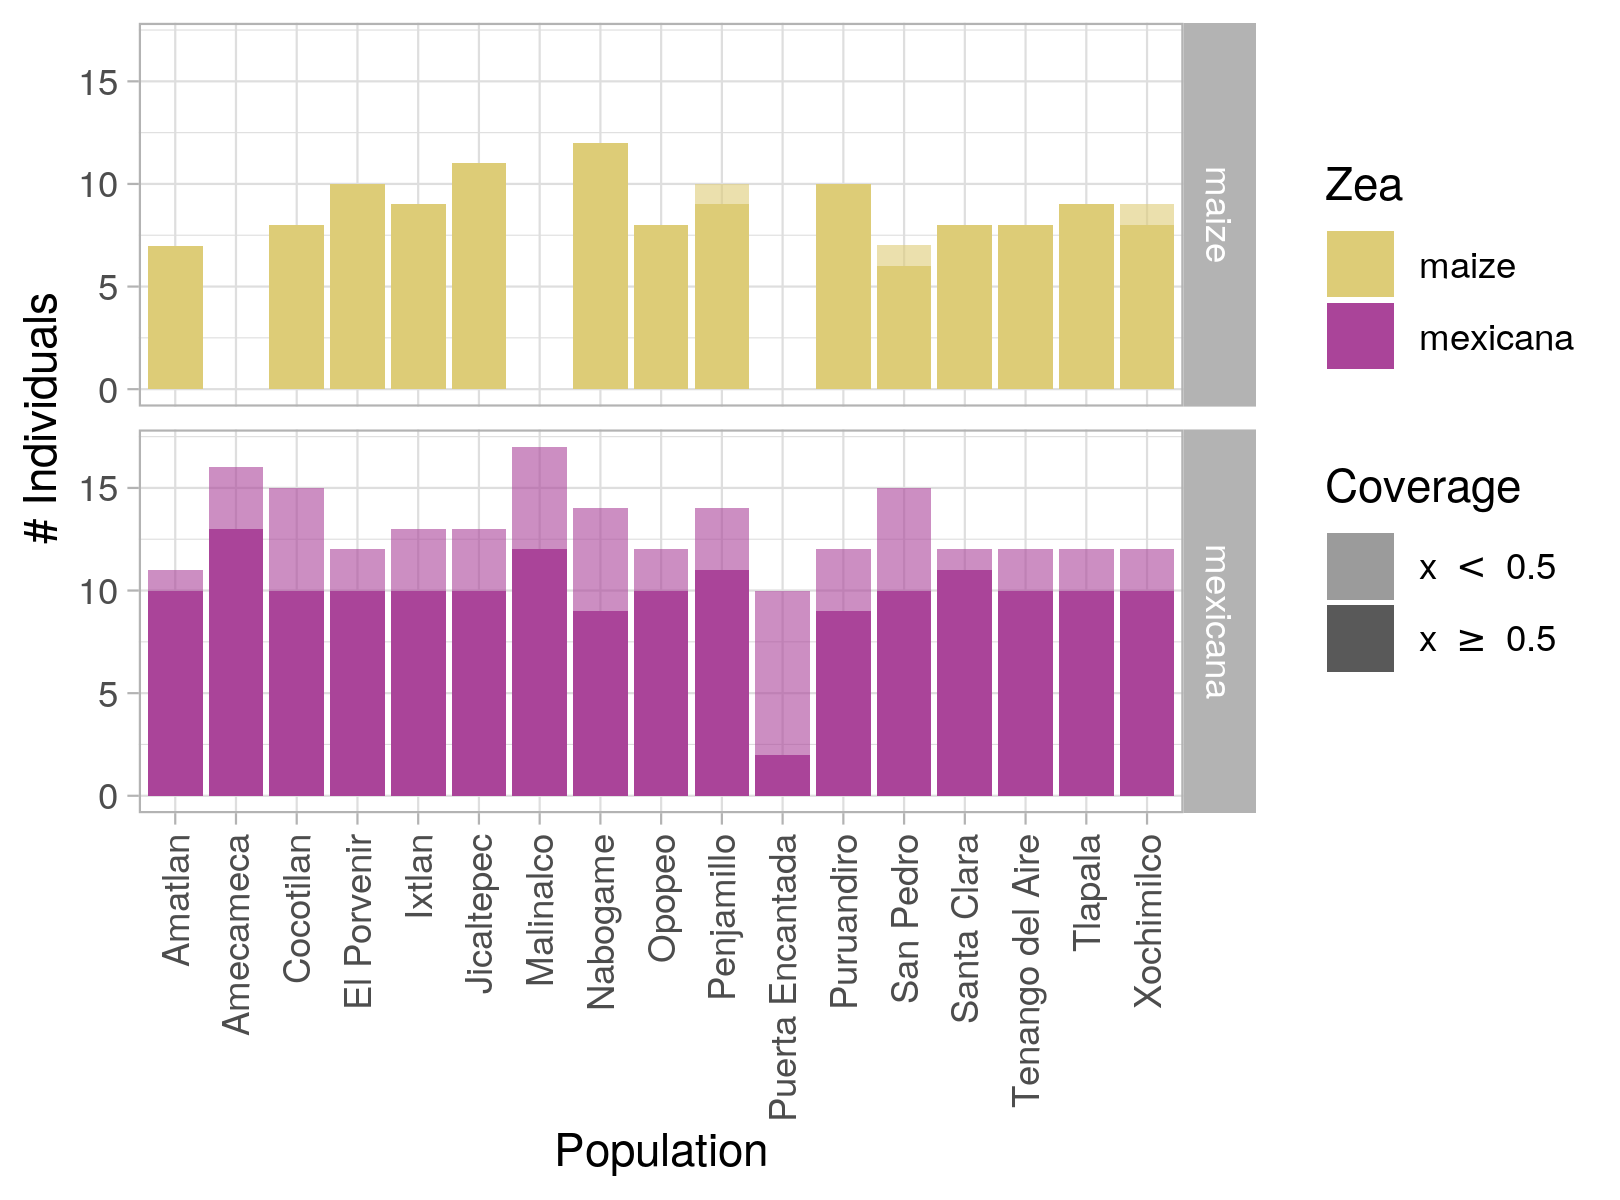
\includegraphics[width=\textwidth]{chapter2/figures/p_seq_counts.png}
	\caption{\color{Gray} \textbf{Number of individuals sequenced per location}. Number of maize (top) and \textit{mexicana} (bottom) individuals sequenced by this study with minimum 0.05x WGS coverage. Amecameca, Malinalco and Puerta Encantada have no paired maize samples and are used as a reference panel for \textit{mexicana} ancestry. For sympatric maize and \textit{mexicana}, only individuals meeting a more stringent 0.5x coverage threshold (shown in darker shading) are included in analyses based on local ancestry inference.}
	\label{sequenced_ind_counts}
\end{figure}

\begin{figure}[ht]
%\begin{figure}[ht]
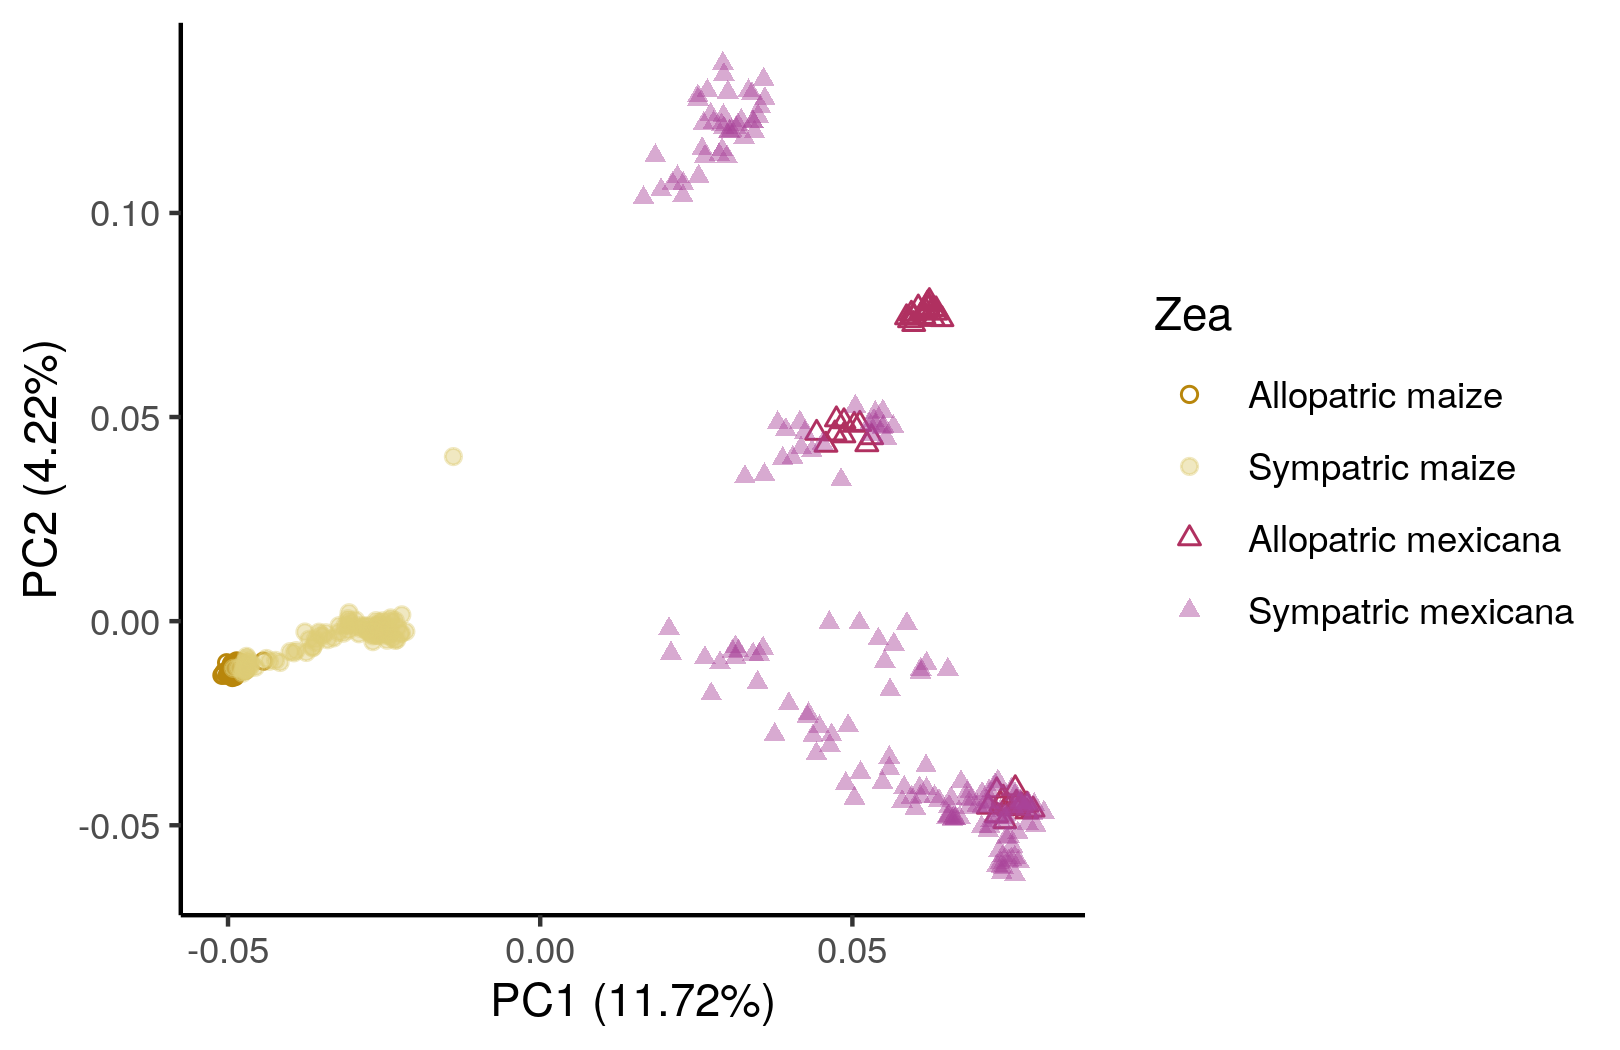
\includegraphics[width=\textwidth]{chapter2/figures/HILO_MAIZE55_pca.png}
\caption{\color{Gray} \textbf{PCA}. First and second principal components from the genomewide genetic covariance matrix relating sympatric and allopatric \ec{(reference)} maize and \mexicana individuals (PCAngsd). PC1 separates maize and \mexicana subspecies while PC2 differentiates genetic clusters within \mexicana.}
\label{pca_maize_mex}
\end{figure}

%\begin{figure}[p]
\begin{figure}[ht]
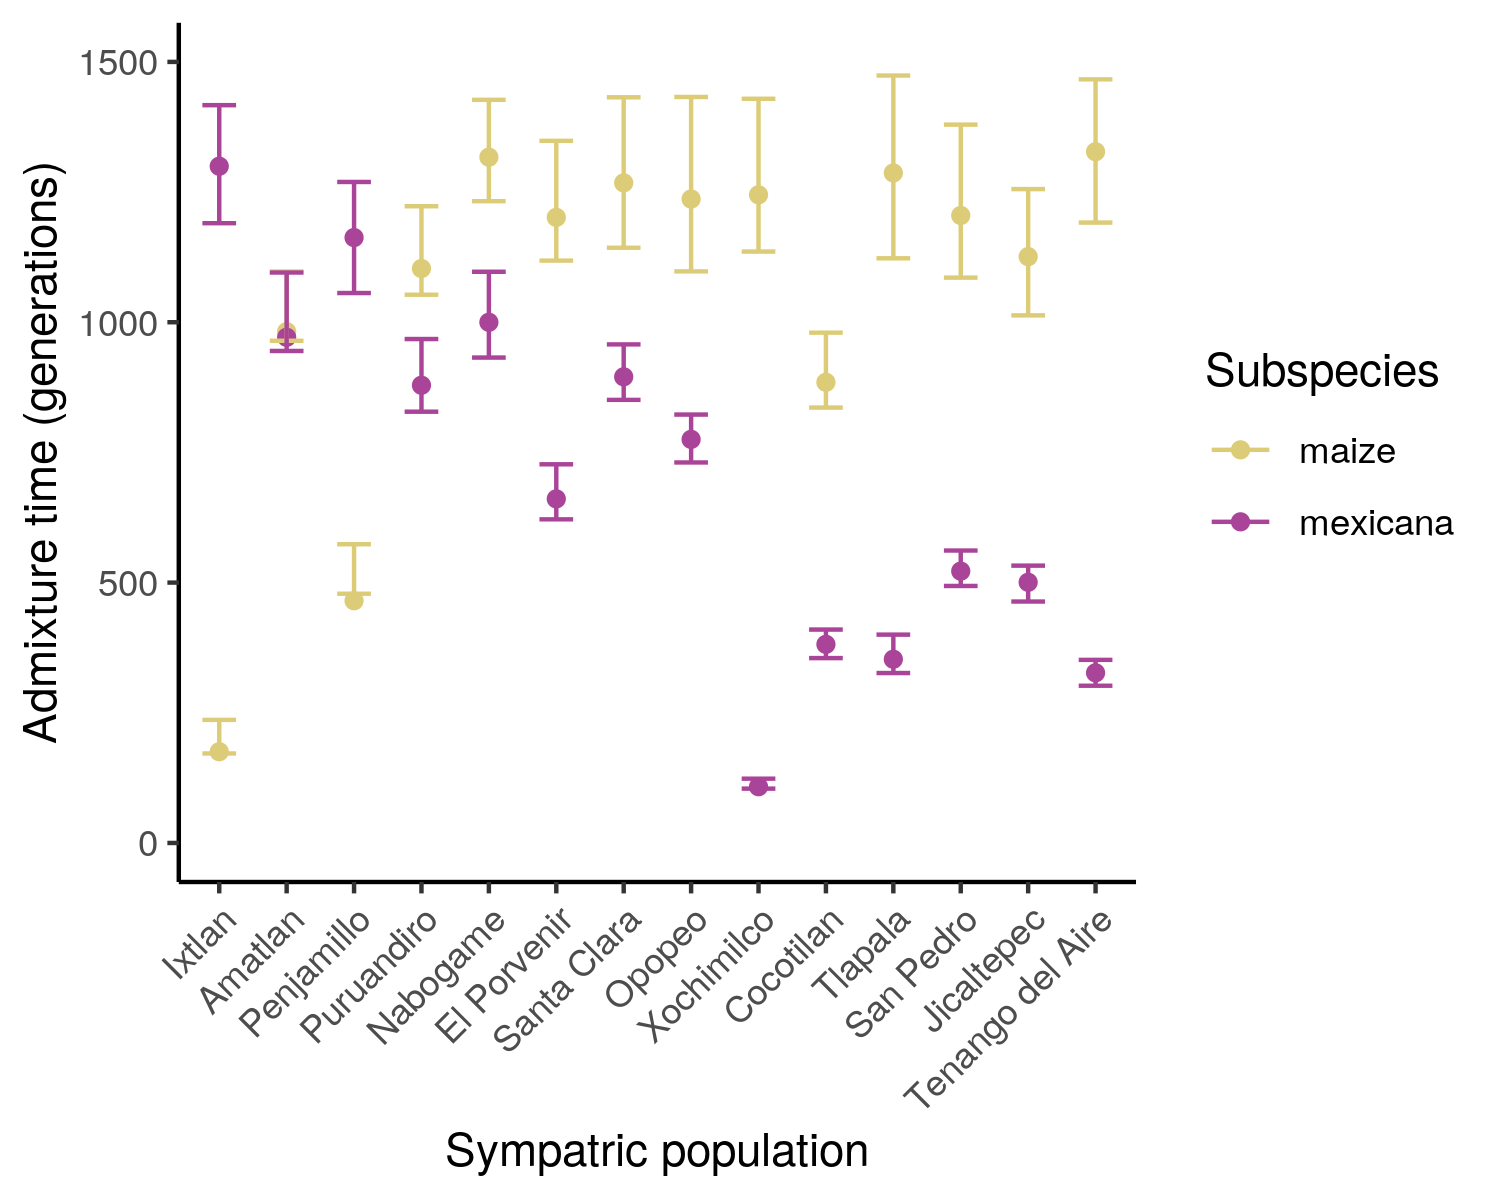
\includegraphics[width=\textwidth]{chapter2/figures/admix_times_Ne10000_yesBoot.png}
\caption{\color{Gray} \textbf{Time since admixture}. Estimated generations since admixture under a single-pulse model for each sympatric maize and \mexicana population, with 95\% percentile confidence intervals based on 100 bootstrap samples of genomic blocks (1,000 SNPs per block). Estimates and bootstraps were produced during ancestry\_hmm model fitting for local ancestry inference. Populations are ordered left to right by increasing elevation.}
\label{time_admix}
\end{figure}

\begin{figure}[ht]
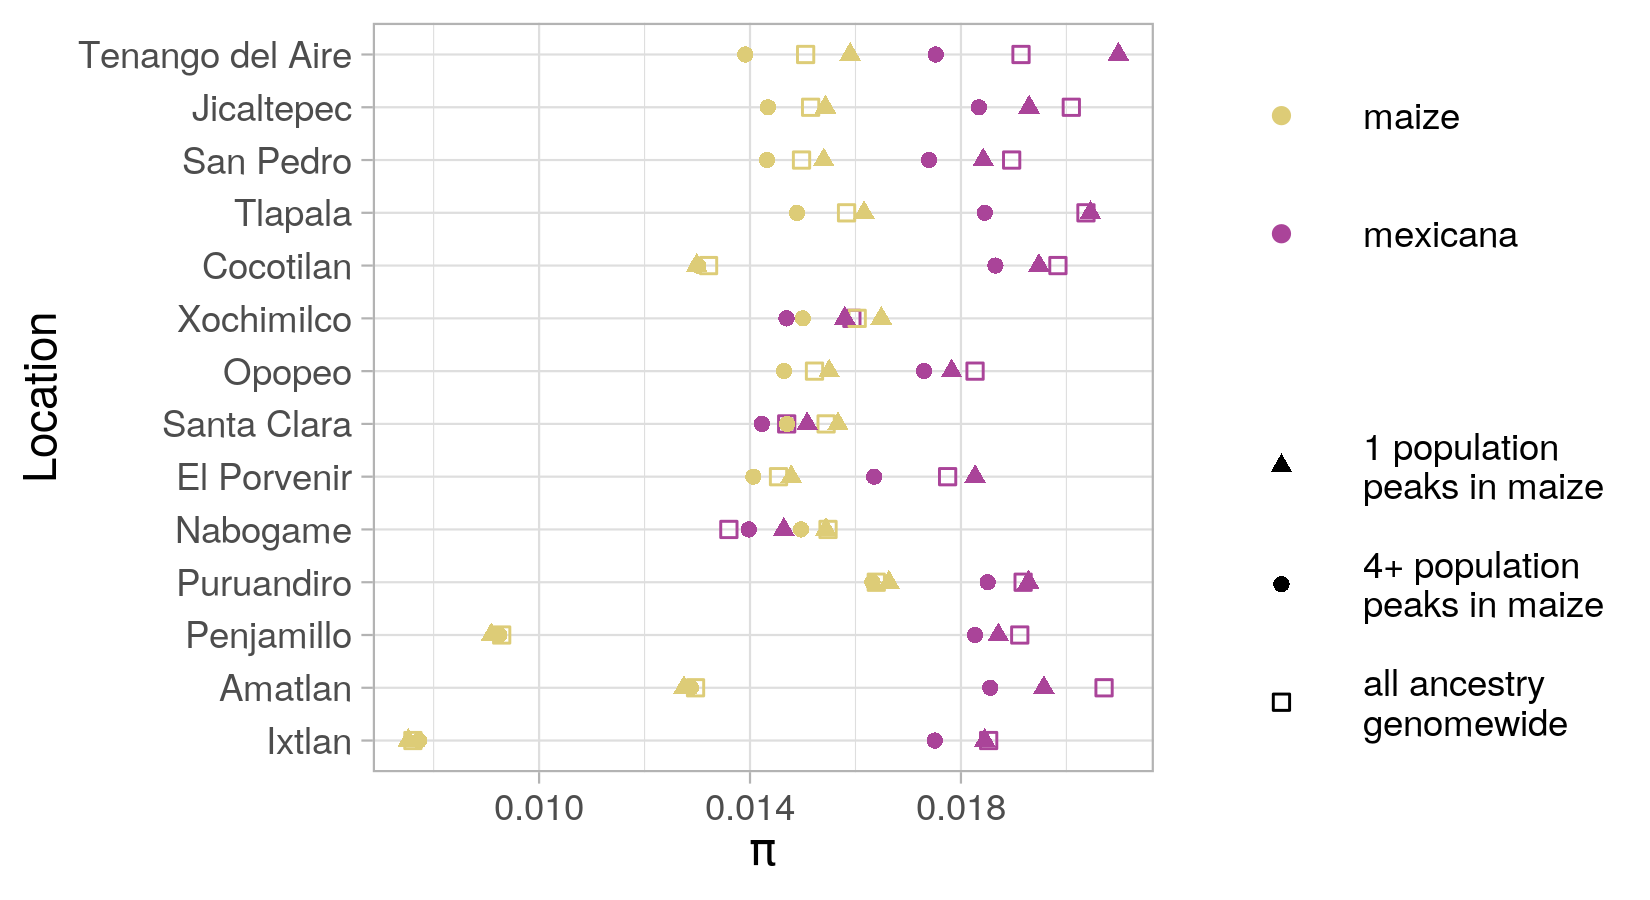
\includegraphics[width=\textwidth]{chapter2/figures/pi_within_mexicana_ancestry_peaks.png}
\caption{\color{Gray} \textbf{Diversity ($\pi$) within \mexicana ancestry} Each point summarises pairwise genetic diversity ($\pi$) for genomic regions with high-confidence homozygous \mexicana ancestry, calculated separately for the maize and \mexicana populations at each sampled location. Within-\mexicana ancestry $\pi$ is calculated and plotted separately for three subsets of the genome: introgression peaks ($>$ 2 s.d. above the mean) found in the focal maize population only, peaks shared between the focal maize and at least 3 other maize populations, and a genomewide estimate.}
\label{pi_mexicana_ancestry_peaks}
\end{figure}

\begin{figure}[ht]
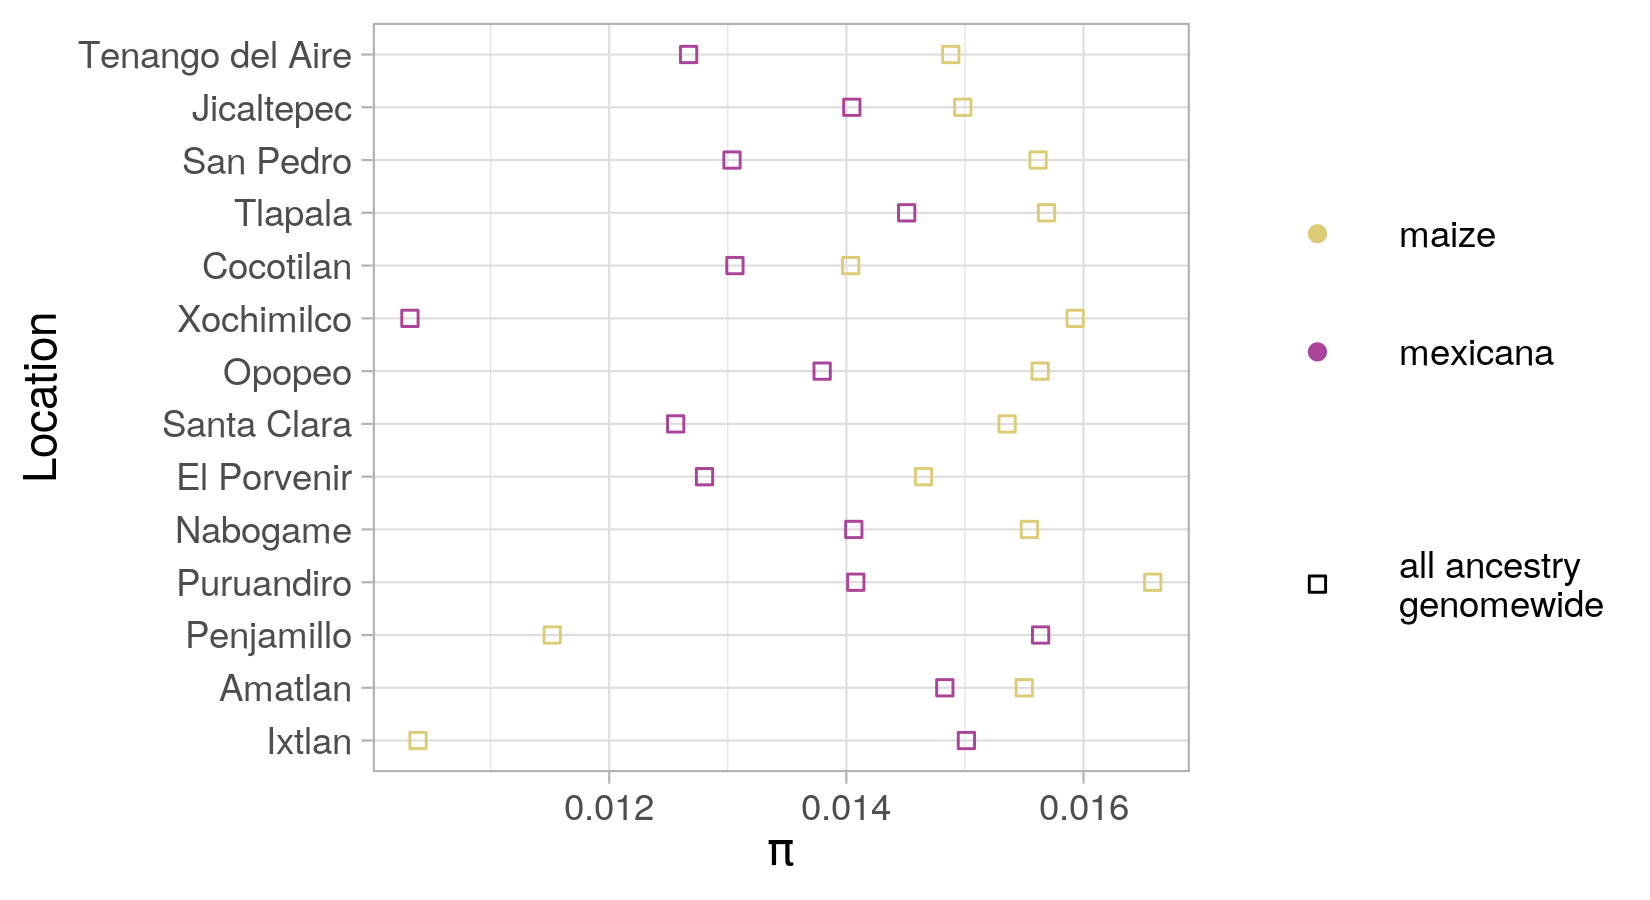
\includegraphics[width=\textwidth]{chapter2/figures/pi_within_maize_ancestry.png}
\caption{\color{Gray} \textbf{Diversity ($\pi$) within maize ancestry} Each point summarises pairwise genetic diversity ($\pi$) for regions genomewide with high-confidence homozygous \mexicana ancestry, calculated separately for the maize and \mexicana populations at each sampled location.}
\label{pi_maize_ancestry}
\end{figure}

%\begin{figure}[p]
\begin{figure}[ht]
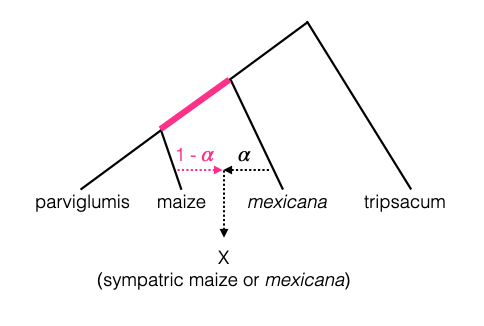
\includegraphics[width=\textwidth]{chapter2/figures/tree_f4_stats.png}
\caption{\color{Gray} \textbf{Population tree} Phylogenetic tree assumed when estimating the ratio of $f_4$ statistics. The pink branch represents the shared drift between maize and parviglumis that is introduced to the focal sympatric population via admixture of proportion $1 - \alpha$. We used only plants from the Amecameca site in our \mexicana reference group for this analysis because that site showed no evidence of previous admixture.}
\label{f4_tree}
\end{figure}

%\begin{figure}[p]
\begin{figure}[ht]
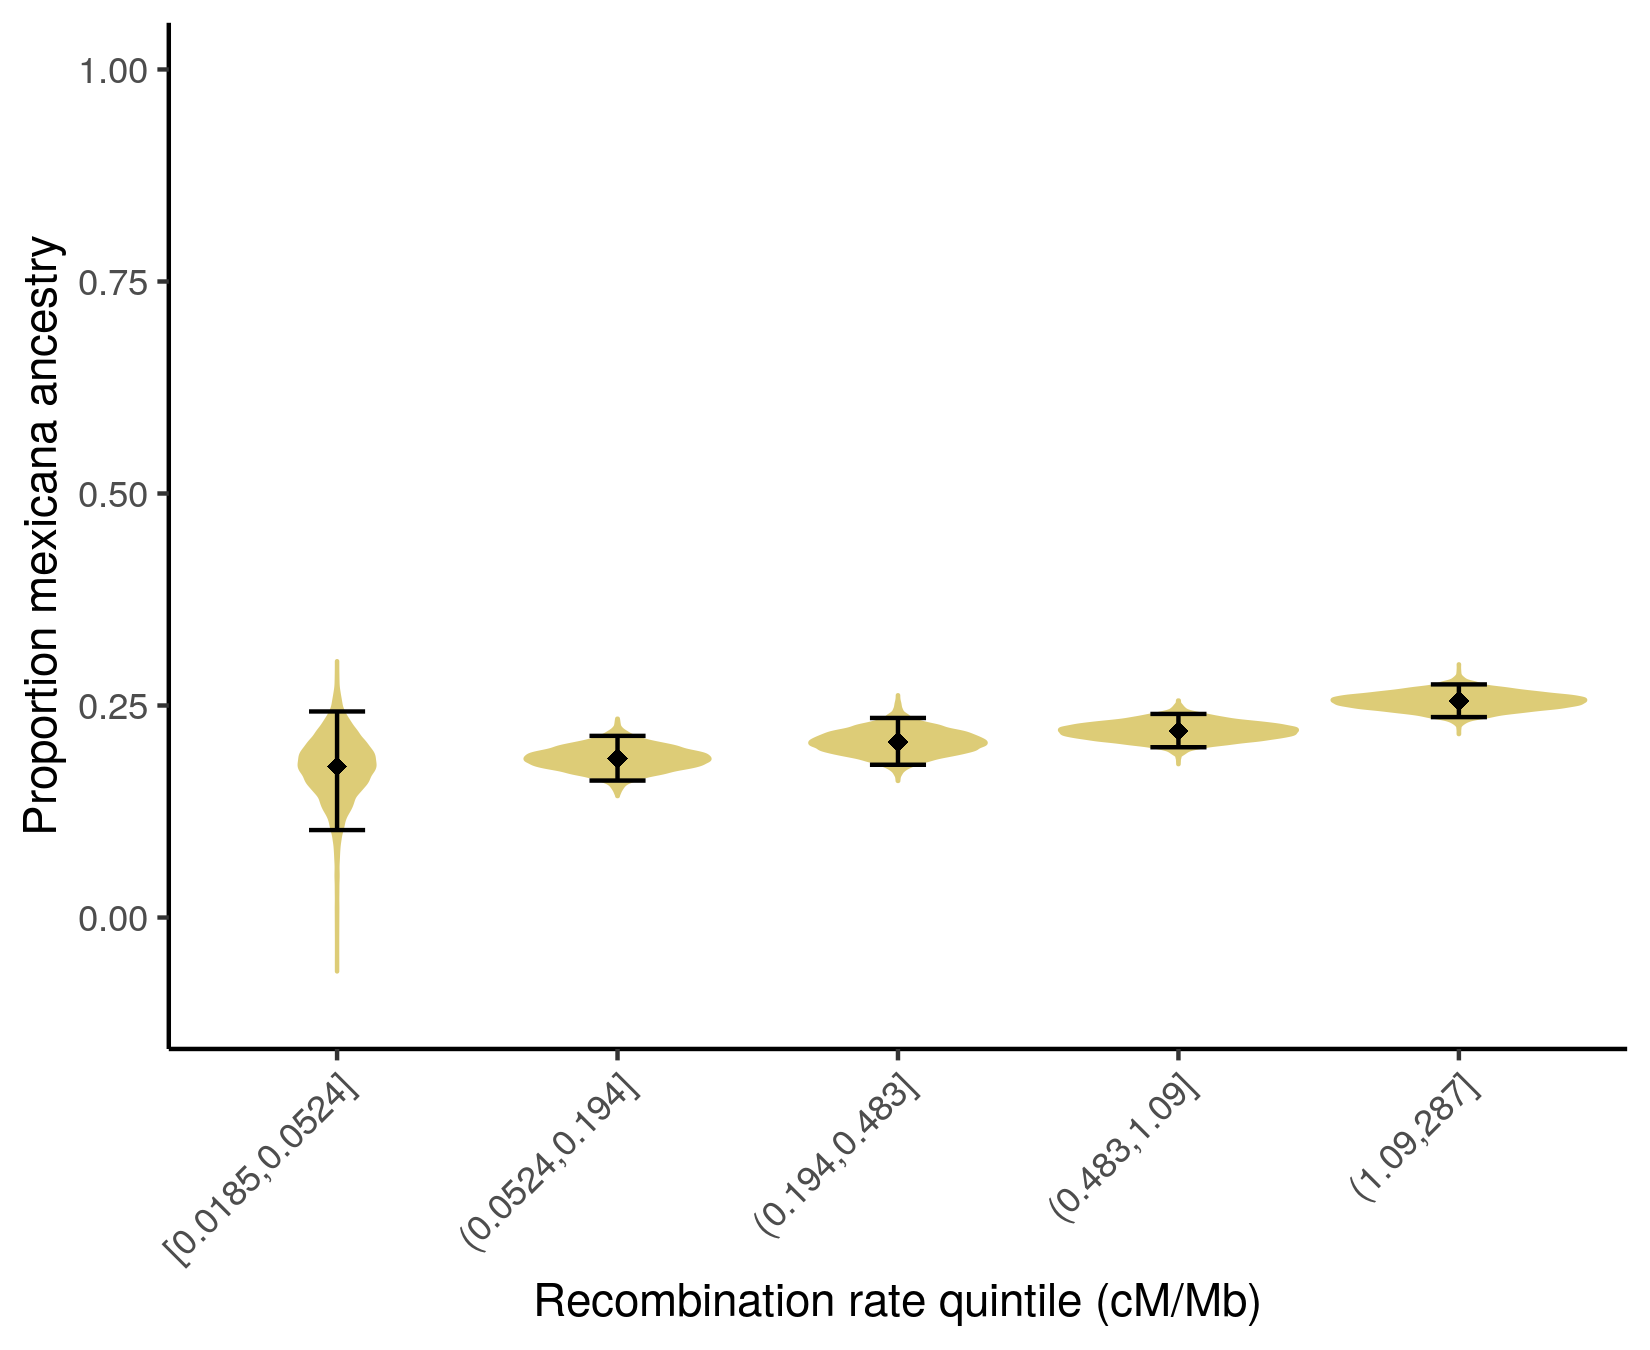
\includegraphics[width=\textwidth]{chapter2/figures/f4_sympatric_maize_pop22_byr5.png}
\caption{\color{Gray} \textbf{$f_4$ ancestry in maize by recombination rate}. Estimated \textit{mexicana} ancestry in sympatric maize landrace samples using $f_4$ ratio. Mean ancestry per recombination rate quintile and 95\% percentile bootstrap confidence interval (n = 10,000) are depicted in black. Violin plots show the density of ancestry estimates for individual bootstraps re-sampled within quintiles.}
\label{f4_maize_by_r}
\end{figure}

%\begin{figure}[p]
\begin{figure}[ht]
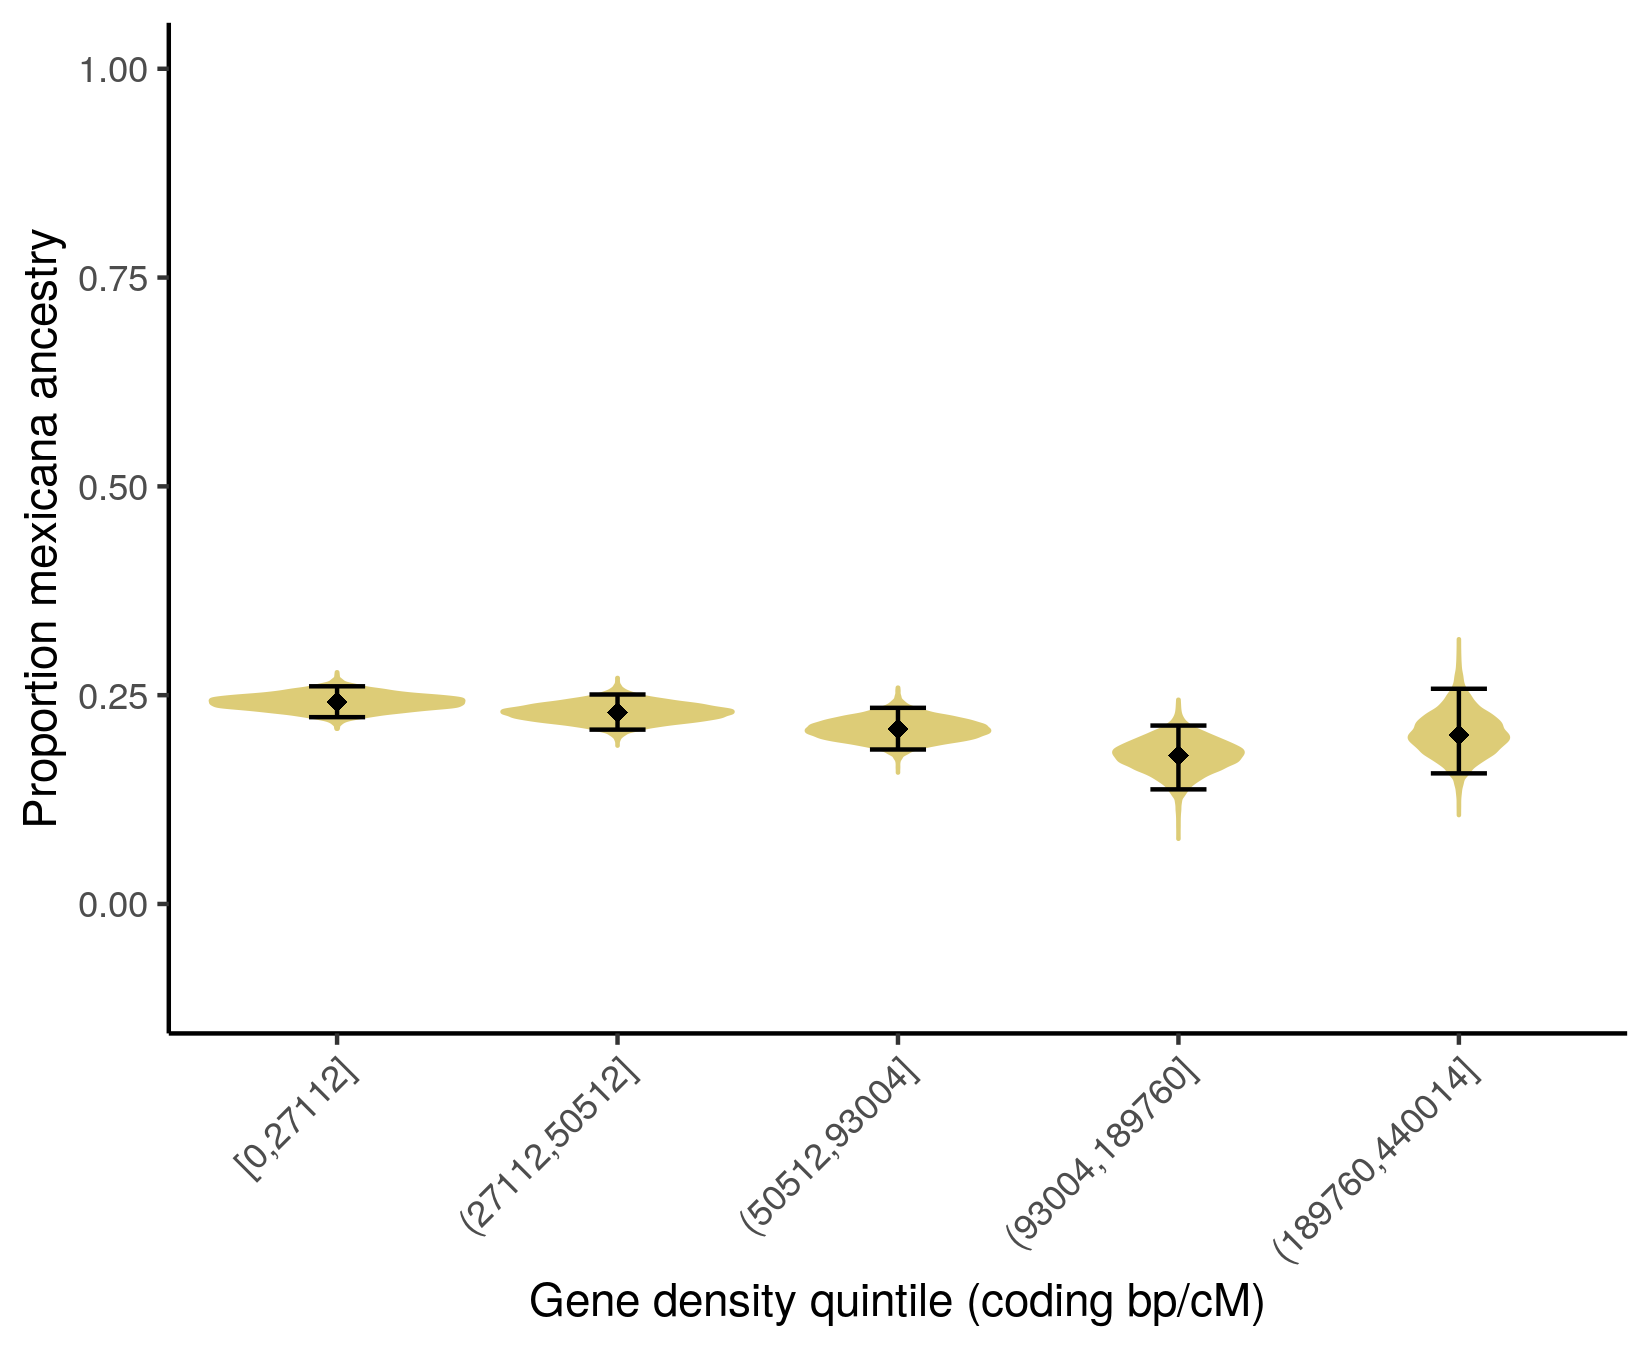
\includegraphics[width=\textwidth]{chapter2/figures/f4_sympatric_maize_pop22_bycd5.png}
\caption{\color{Gray} \textbf{$f_4$ ancestry in maize by coding bp per cM}. Estimated \textit{mexicana} ancestry in sympatric maize landrace samples using $f_4$ ratio. Mean ancestry for each coding bp/cM quintile and 95\% percentile bootstrap confidence interval (n = 10,000) are depicted in black. Violin plots show the density of ancestry estimates for individual bootstraps re-sampled within quintiles.}
\label{f4_maize_by_cd}
\end{figure}

\begin{figure}[ht]
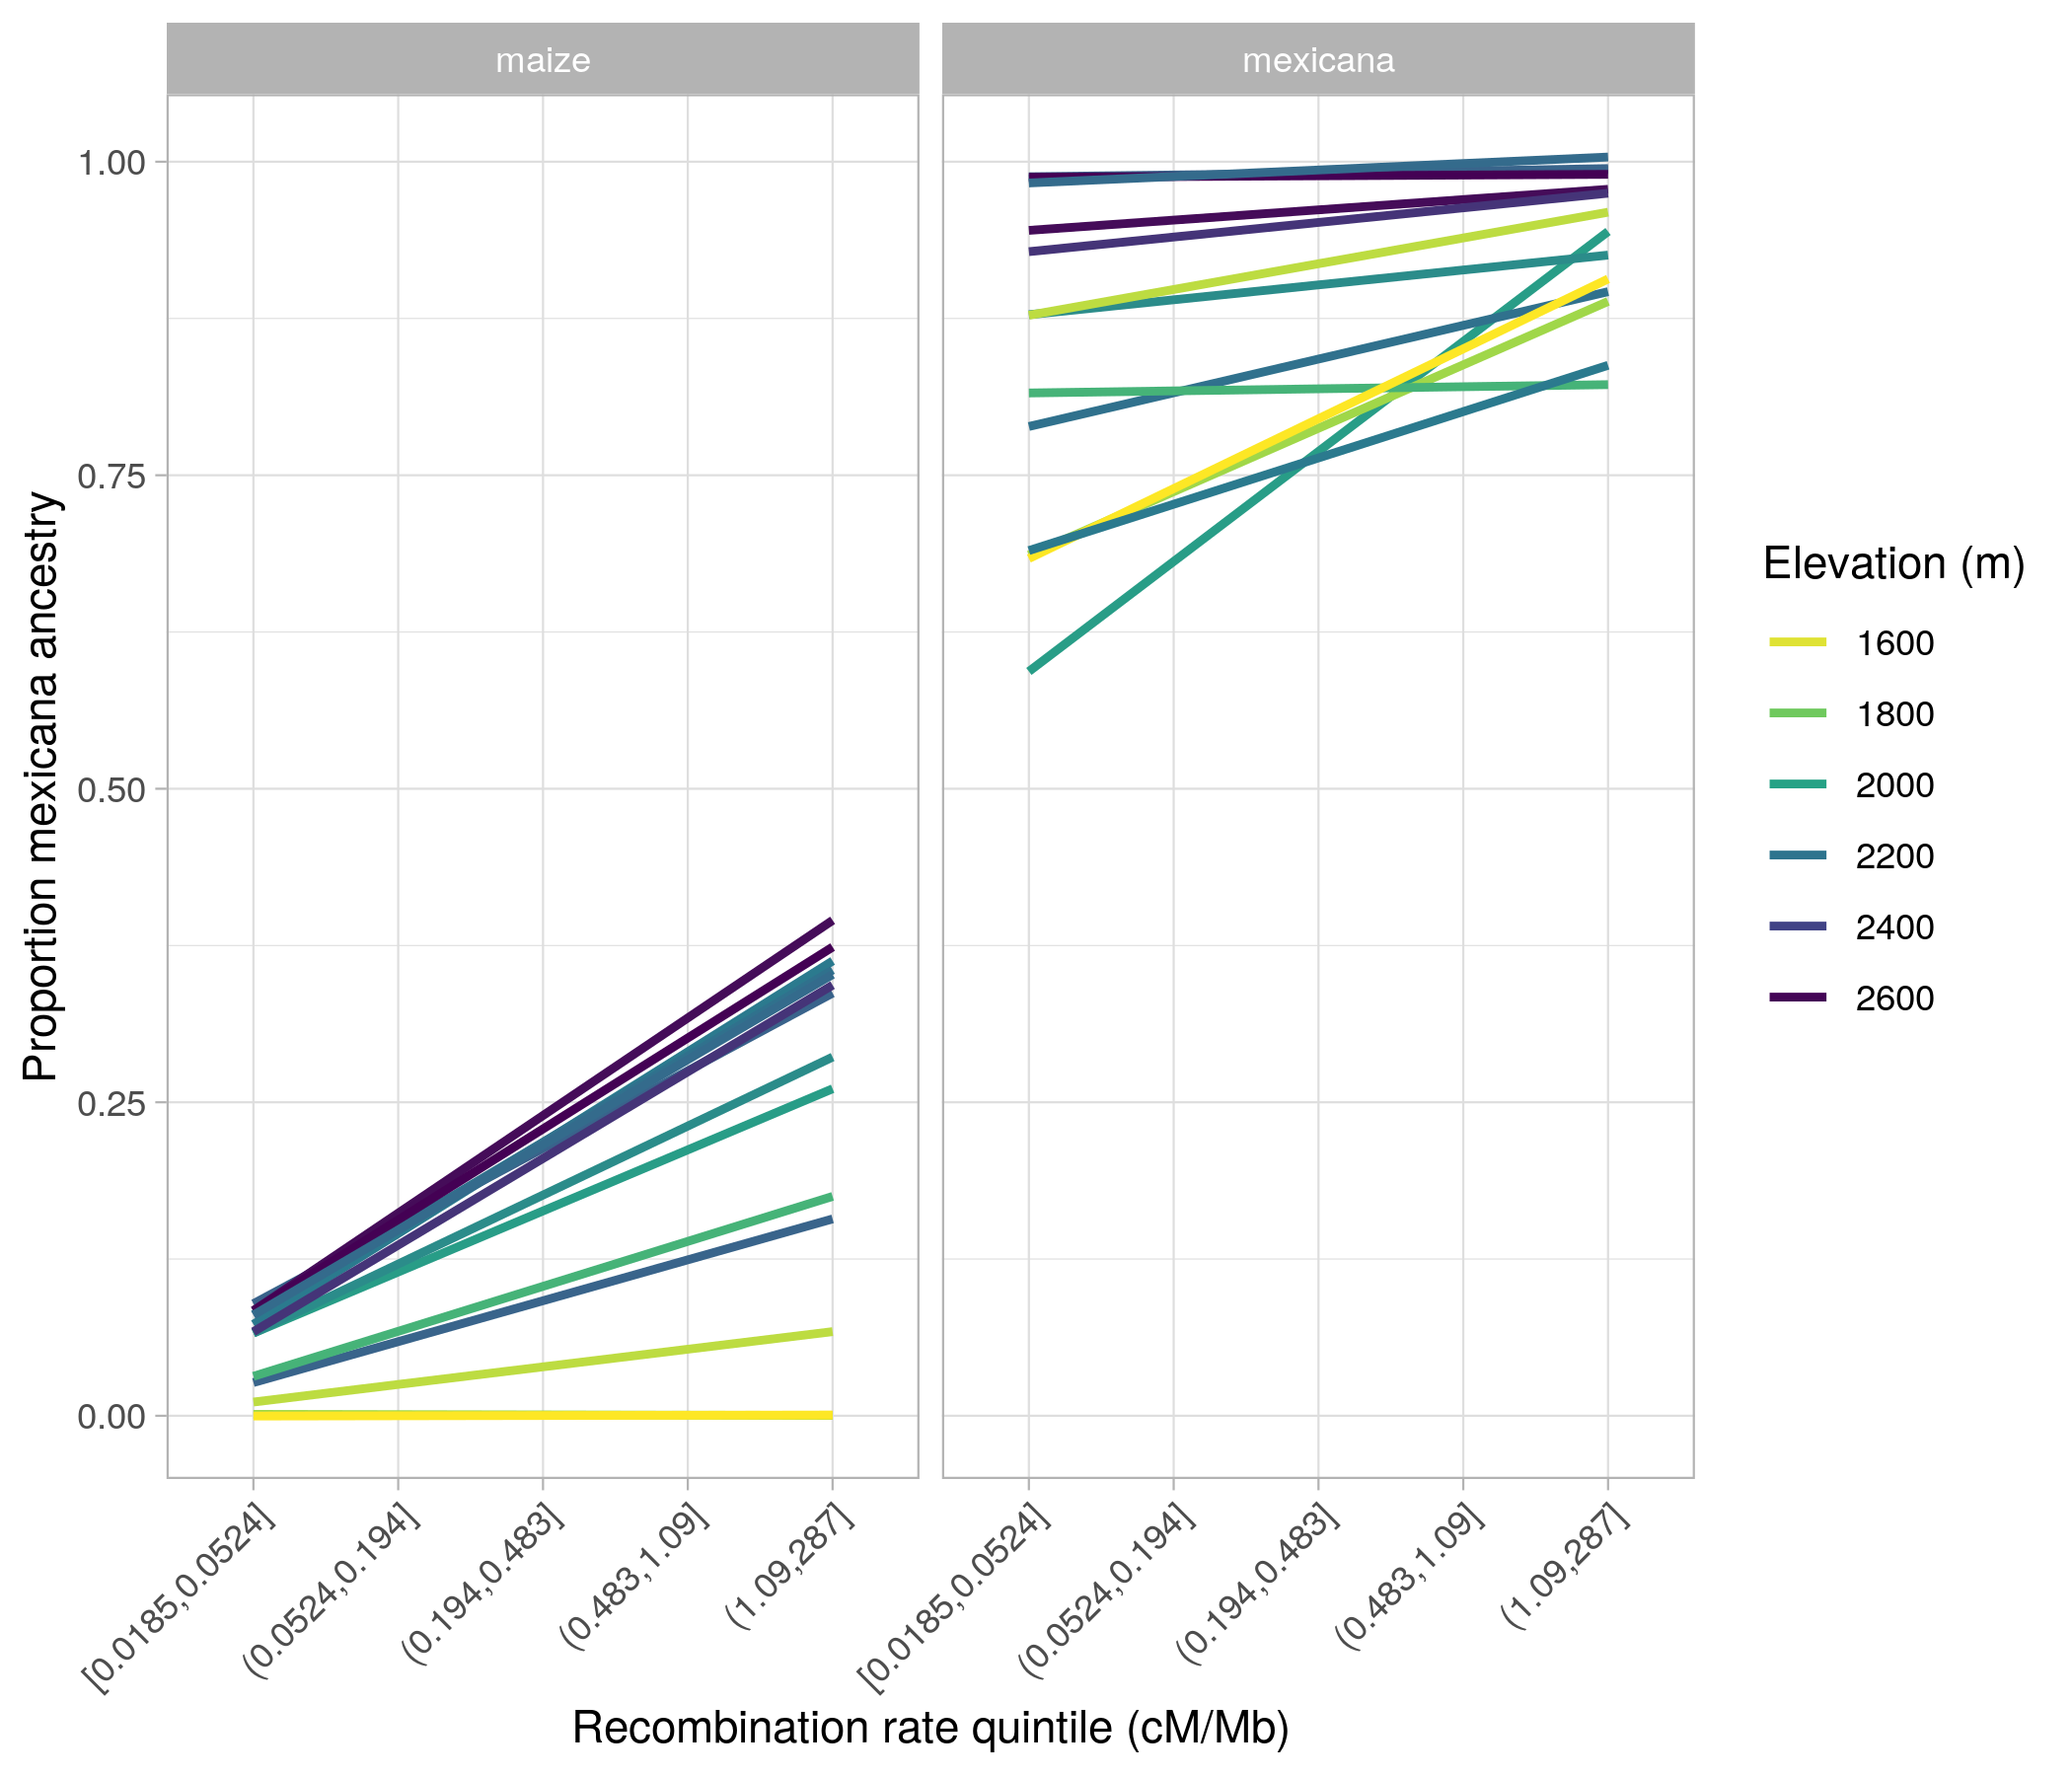
\includegraphics[width=\textwidth]{chapter2/figures/K2_by_r_bootstrap_lm_elevation_color_elev.png}
\caption{\color{Gray} \textbf{\textit{Mexicana} ancestry across recombination quintiles by elevation}. Estimated linear relationship between proportion \mexicana ancestry (NGSAdmix) and recombination rate quintile for each sympatric population, colored by elevation. Linear models were fit using \textit{lm()} in R on individuals' ancestry estimates per quintile.}
\label{K2_by_r_elev_lm}
\end{figure}

%\begin{figure}[p]
\begin{figure}[ht]
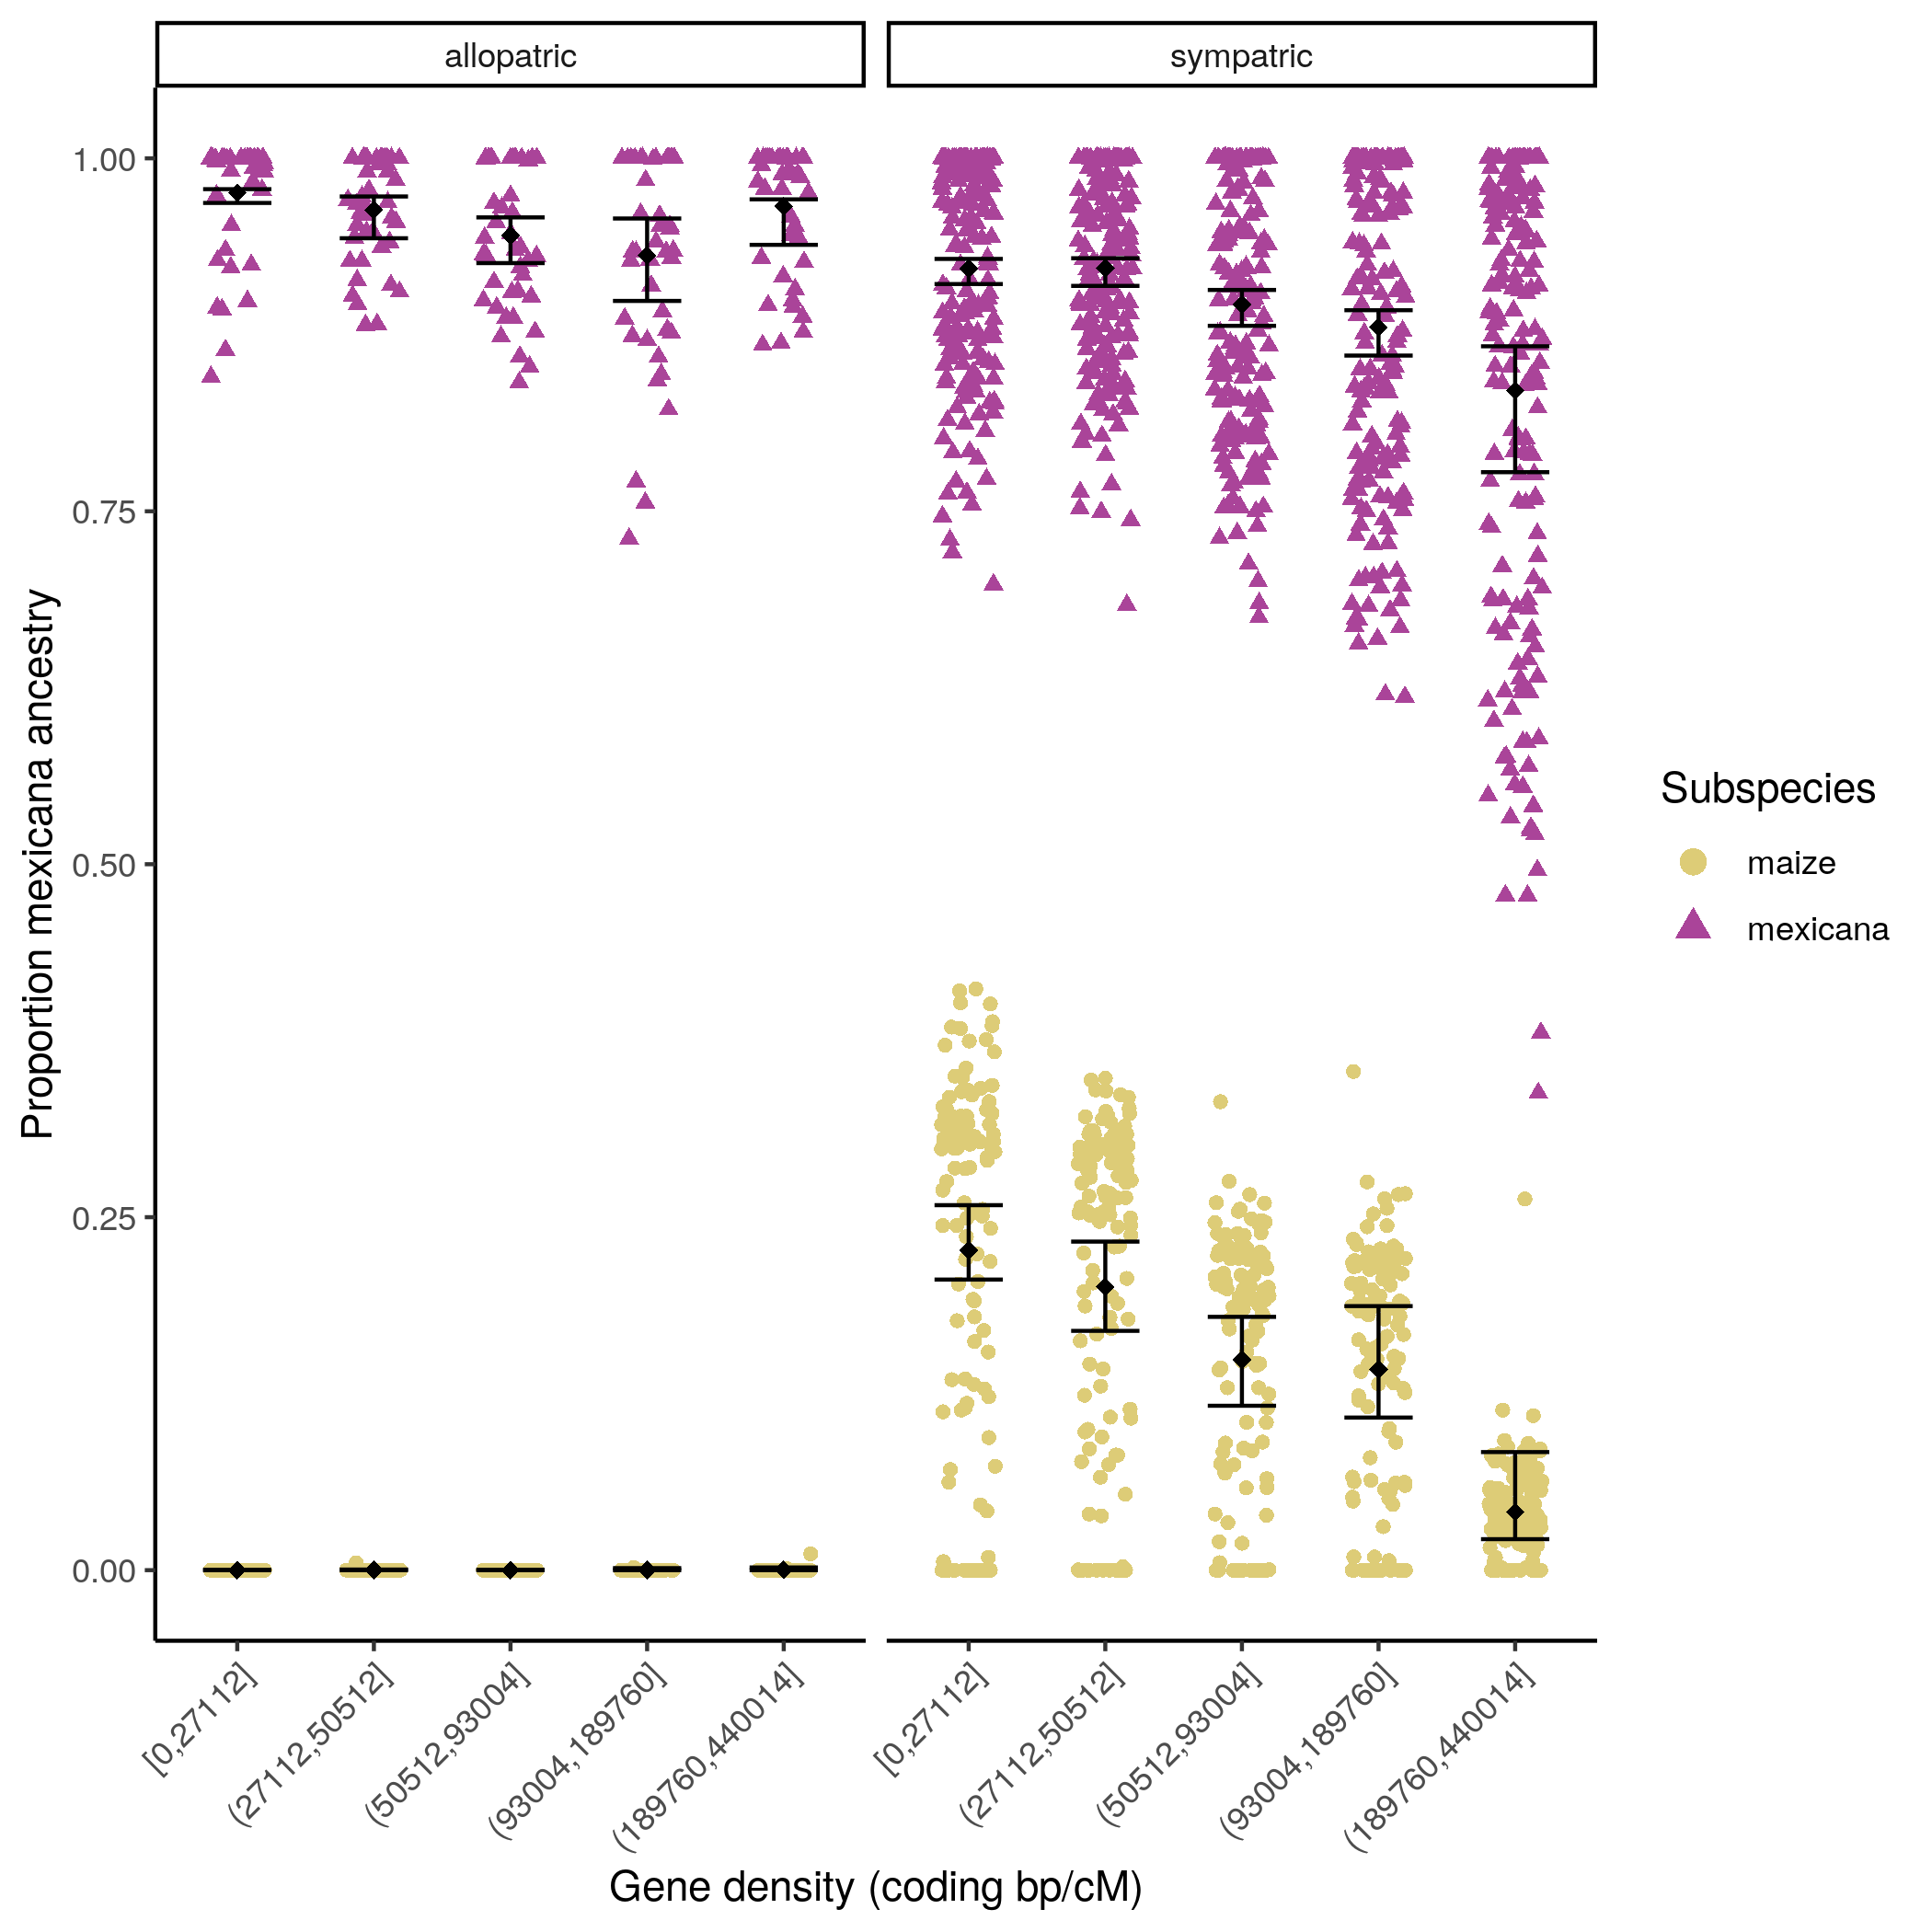
\includegraphics[width=\textwidth]{chapter2/figures/K2_by_cd_bootstrap_sympatric_and_allopatric.png}
\caption{\color{Gray} \textbf{\textit{Mexicana} ancestry by coding bp per cM}. Inferred \textit{mexicana} ancestry in  allopatric reference populations (left) and sympatric maize and \textit{mexicana} populations (right) using NGSAdmix (K=2) by coding density quintiles. Group mean and 95\% percentile bootstrap confidence interval (n = 100) are depicted in black. Ancestry estimates for each individual are shown as points, colored by \textit{Zea} subspecies, and points are jittered for better visualization.}
\label{K2_by_cd}
\end{figure}


%\begin{figure}[p]
\begin{figure}[ht]
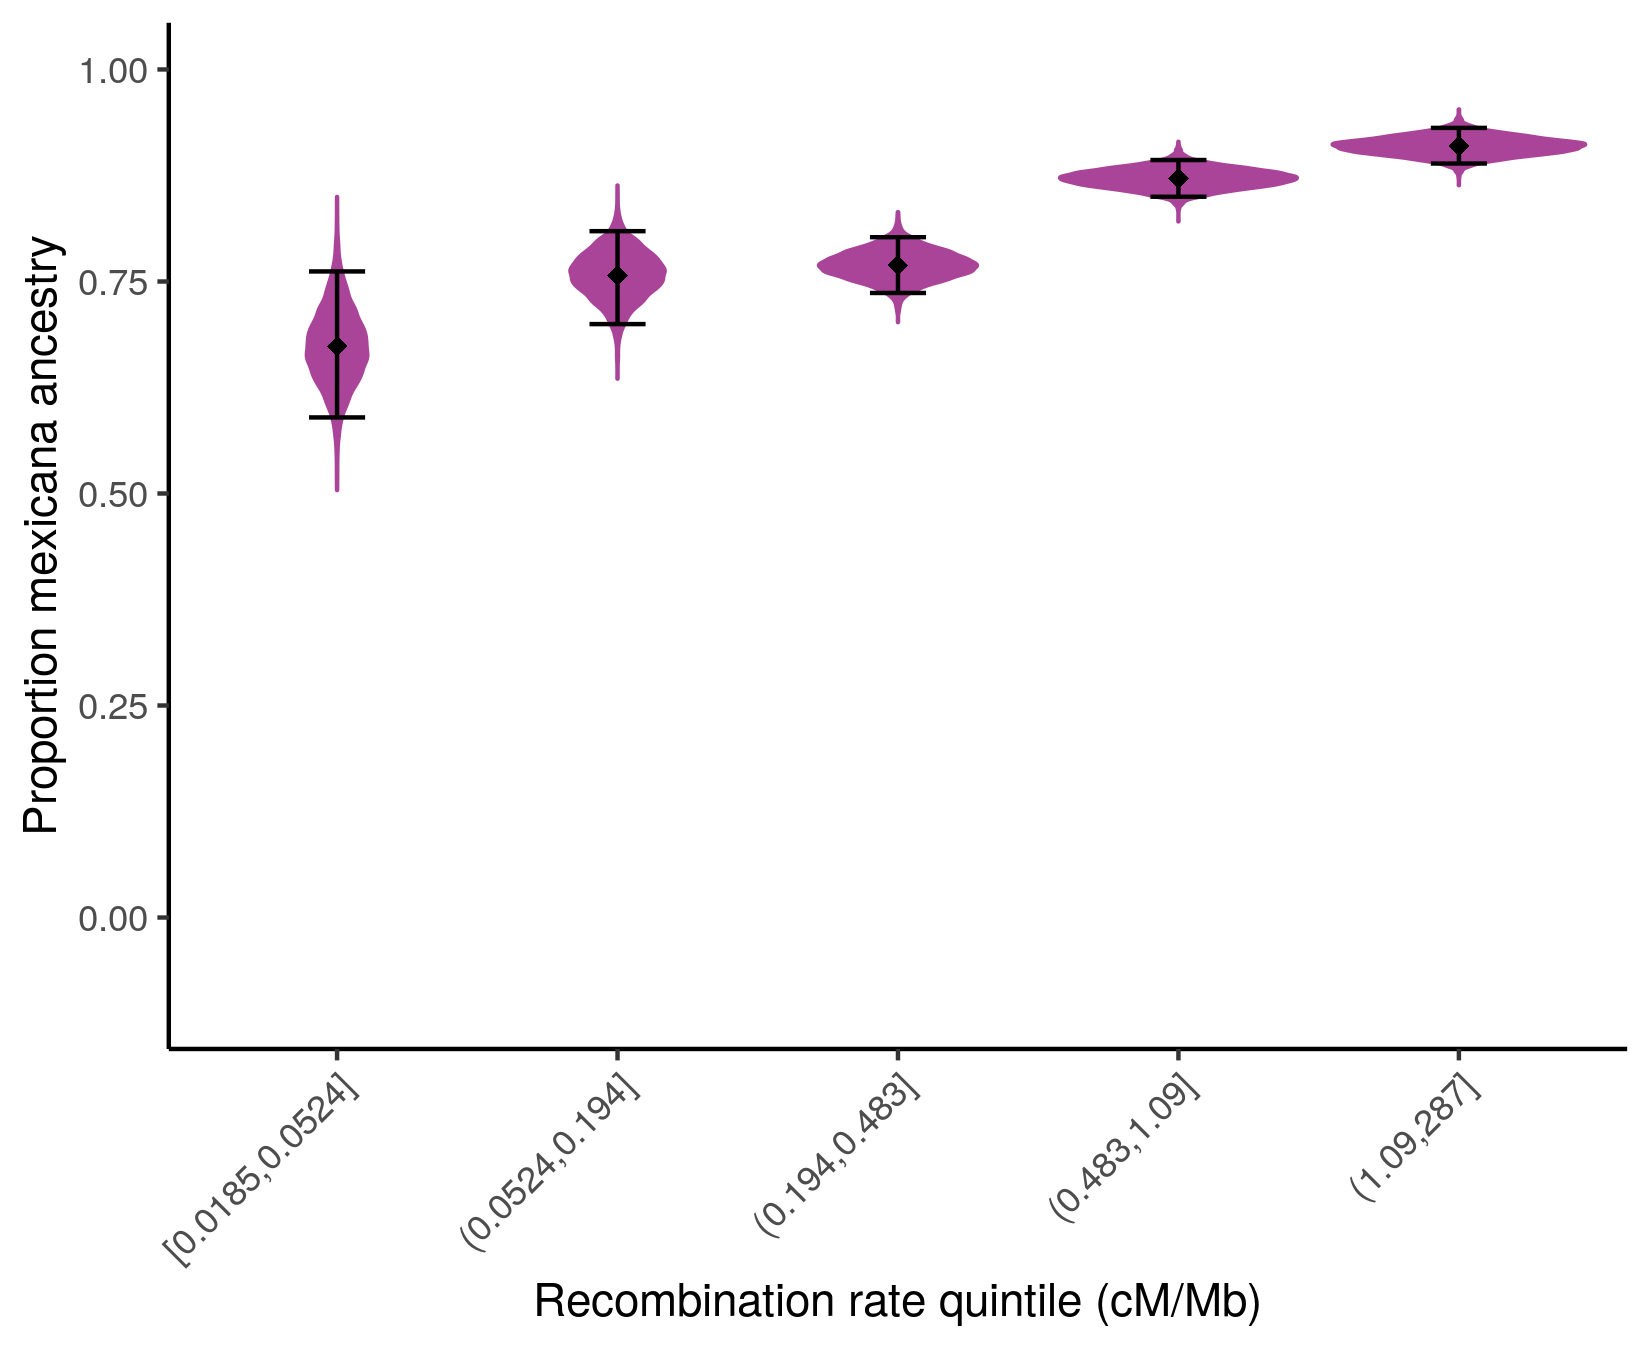
\includegraphics[width=\textwidth]{chapter2/figures/f4_sympatric_mexicana_pop22_byr5.png}
\caption{\color{Gray} \textbf{$f_4$ ancestry in maize by recombination rate}. Estimated \textit{mexicana} ancestry in sympatric mexicana samples using $f_4$ ratio. Mean ancestry per recombination rate quintile and 95\% percentile bootstrap confidence interval (n = 10,000) are depicted in black. Violin plots show the density of ancestry estimates for individual bootstraps re-sampled within quintiles.}
\label{f4_mexicana_by_r}
\end{figure}

%\begin{figure}[p]
\begin{figure}[ht]
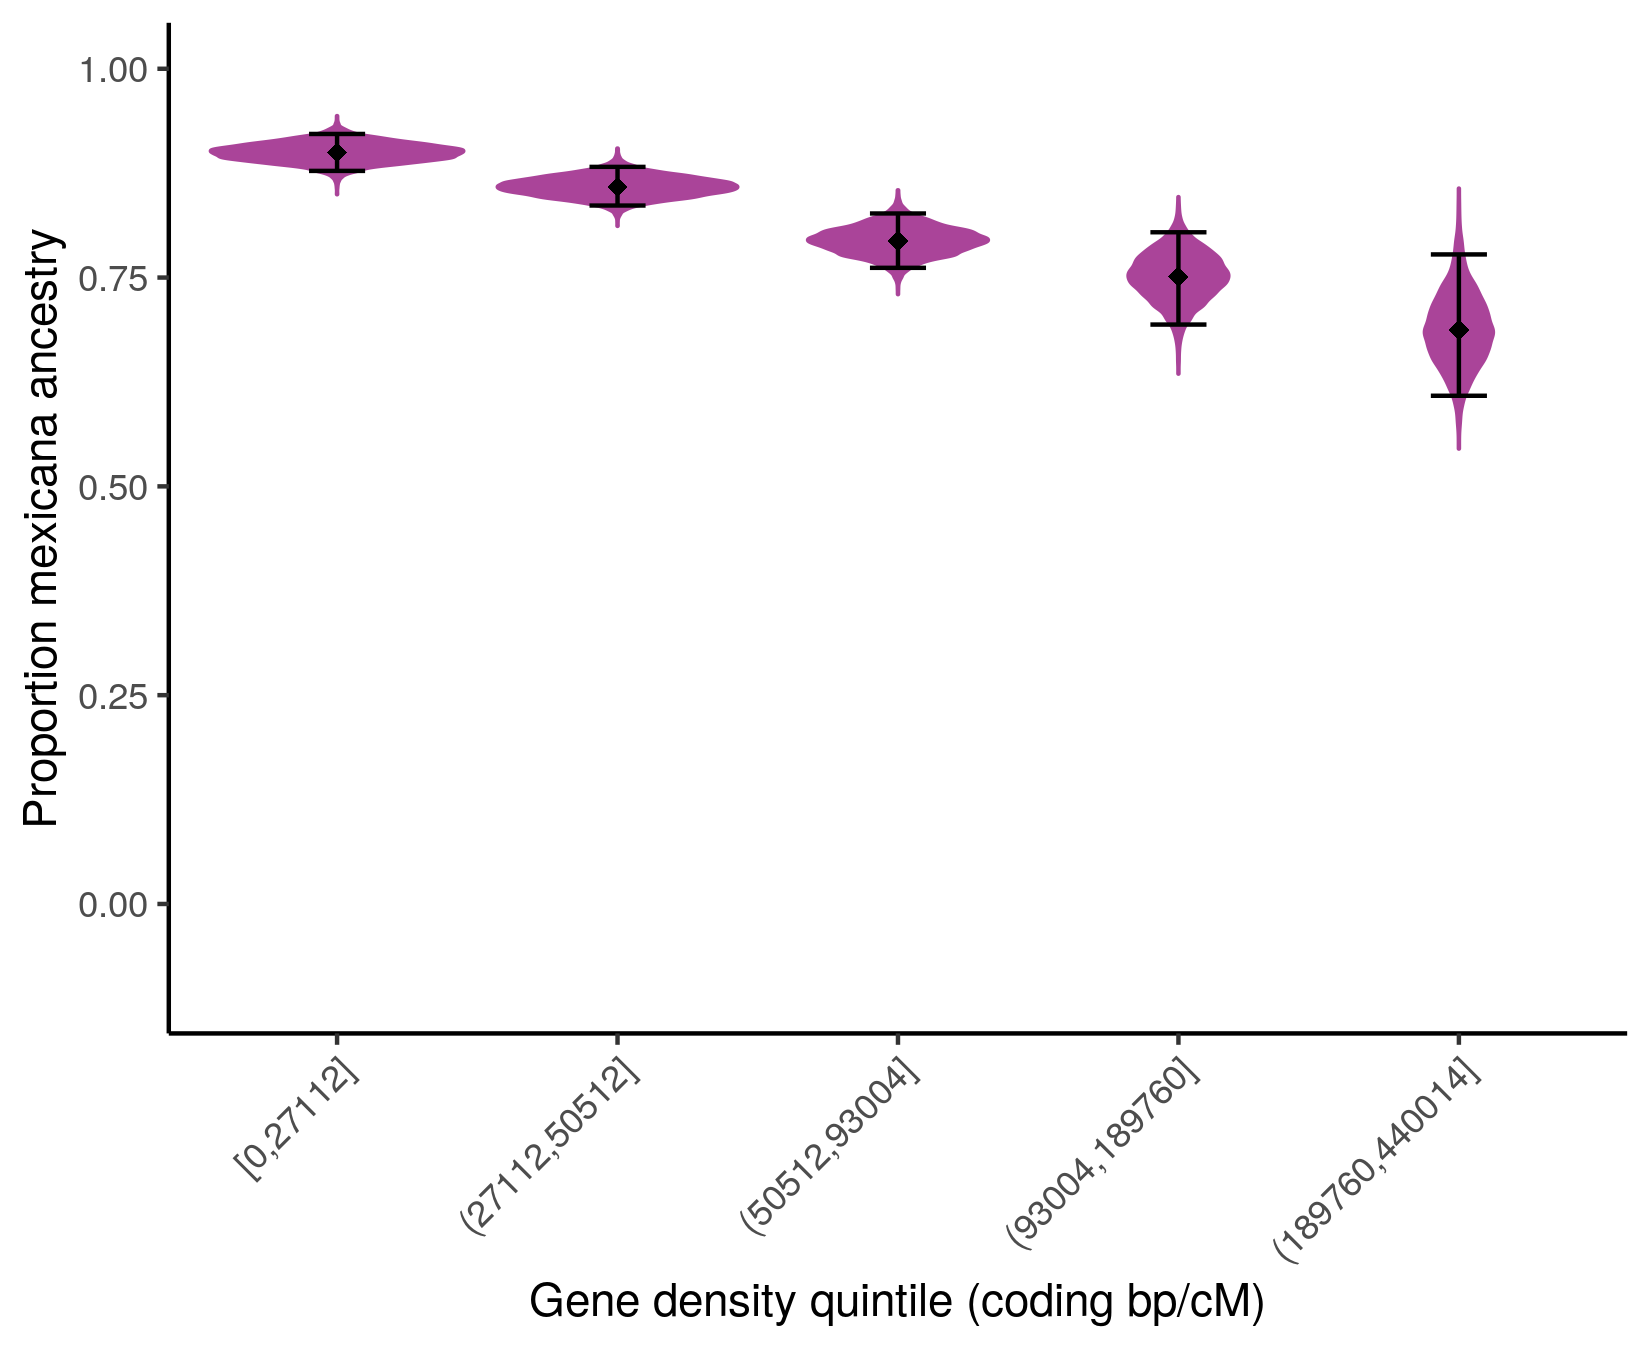
\includegraphics[width=\textwidth]{chapter2/figures/f4_sympatric_mexicana_pop22_bycd5.png}
\caption{\color{Gray} \textbf{$f_4$ ancestry in mexicana by coding bp per cM}. Estimated \textit{mexicana} ancestry in sympatric mexicana samples using $f_4$ ratio. Mean ancestry for each coding bp/cM quintile and 95\% percentile bootstrap confidence interval (n = 10,000) are depicted in black. Violin plots show the density of ancestry estimates for individual bootstraps re-sampled within quintiles.}
\label{f4_mexicana_by_cd}
\end{figure}


%\begin{figure}[p]
\begin{figure}[ht]
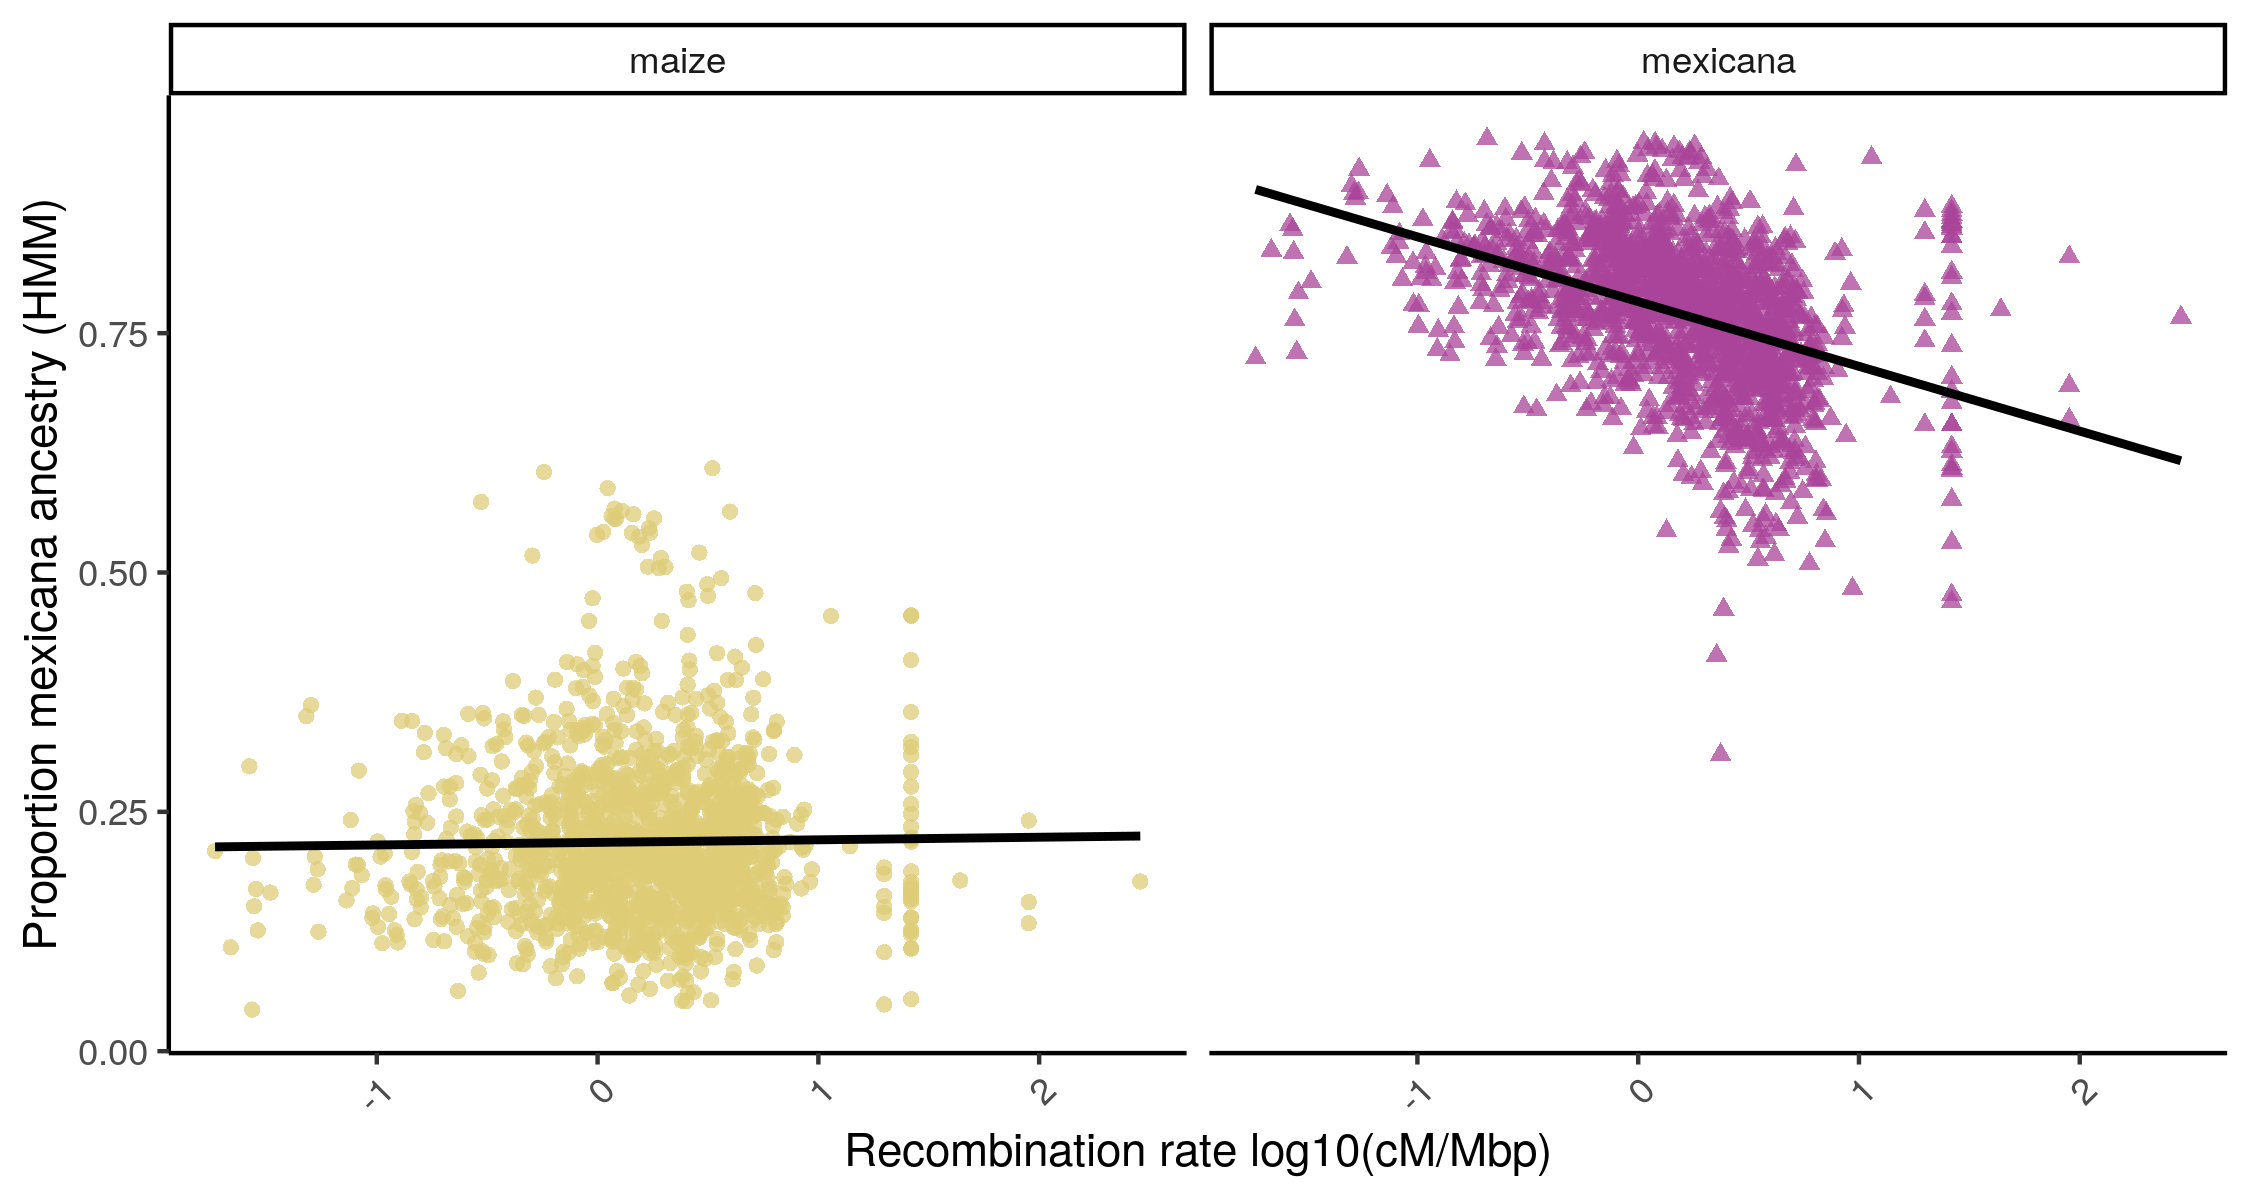
\includegraphics[width=\textwidth]{chapter2/figures/local_anc_by_r_continuous.png}
\caption{\color{Gray} \textbf{Local \mexicana ancestry in 1 cM windows by recombination rate}. Estimated \textit{mexicana} ancestry in sympatric maize and \mexicana samples using ancestry\_hmm. Each point is a 1 cM genomic window and the line shows the best linear model fit for mean \mexicana ancestry by recombination rate on a log scale.}
\label{local_ancestry_mexicana_by_log10r}
\end{figure}

\begin{figure}[ht]
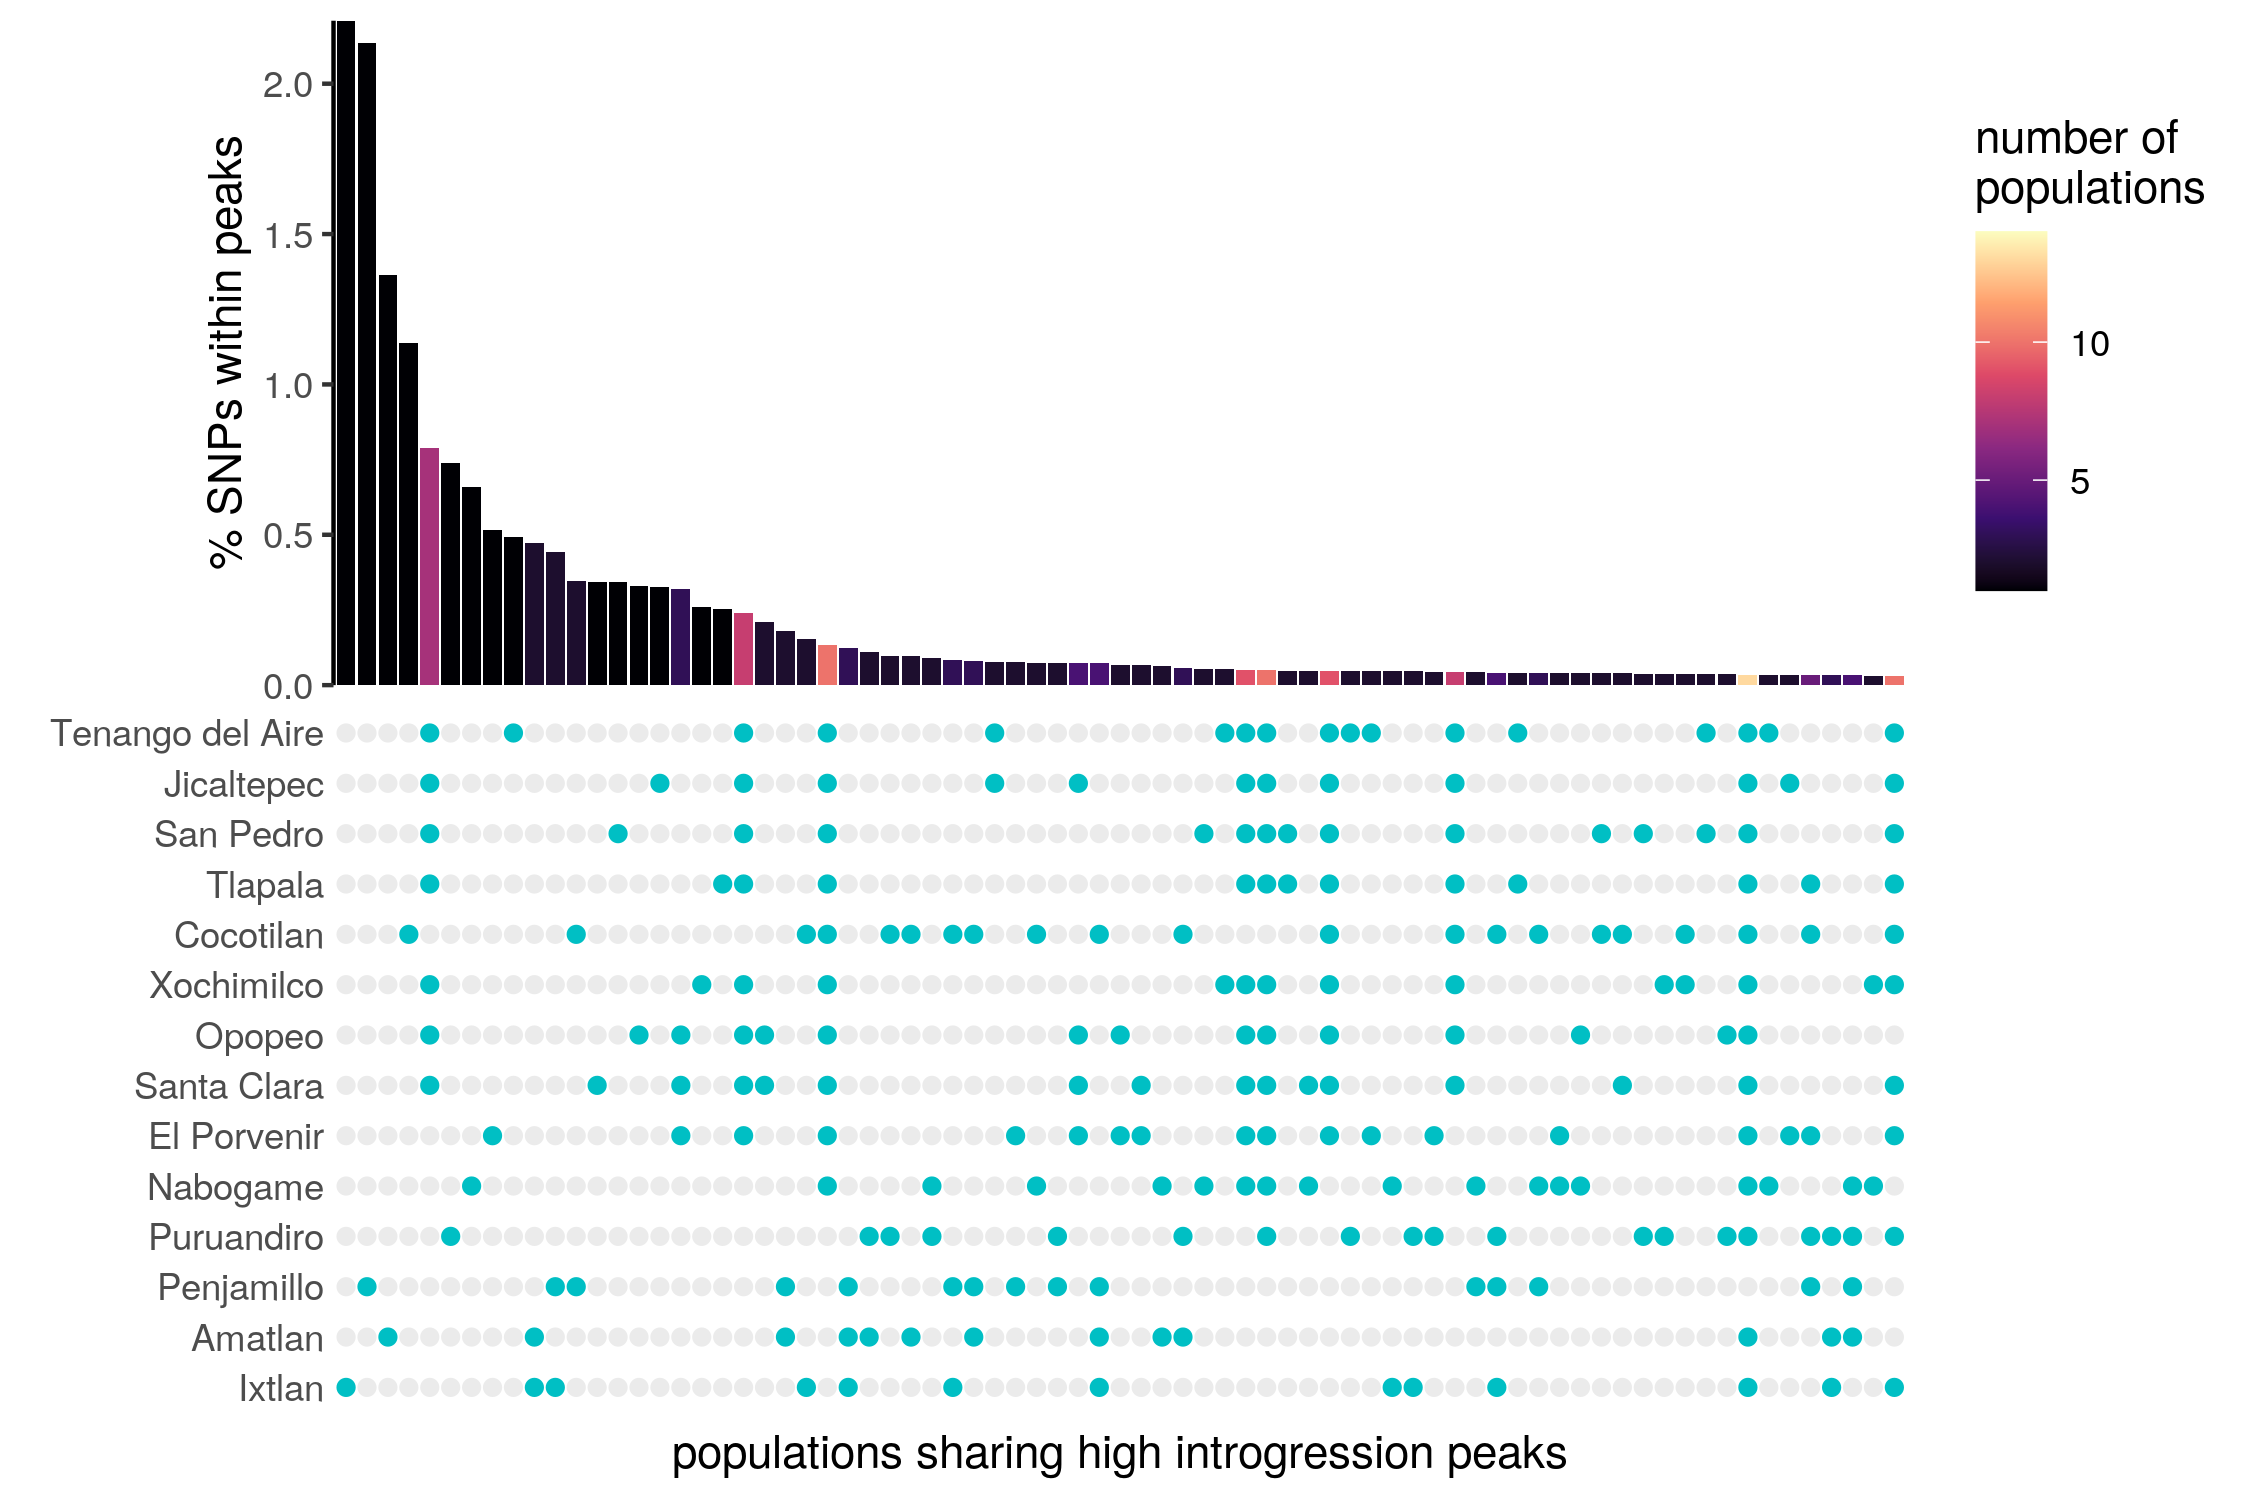
\includegraphics[width=\textwidth]{chapter2/figures/combmatrix_peak_sharing_maize.png}
\caption{\color{Gray} \textbf{High introgression peaks shared across sympatric maize populations} Here we show the 75 most common combinations of populations that share ancestry peaks (introgressed ancestry $>$ 2 s.d. above each population's mean ancestry). Bar height represents the percent of SNPs genomewide within peaks shared by the populations highlighted in blue below. Populations are ordered from high (top) to low elevation. See \ref{combmatrix_peaks_mexicana} for sympatric \mexicana equivalent visualization.}
\label{combmatrix_peaks_maize}
\end{figure}

\begin{figure}[ht]
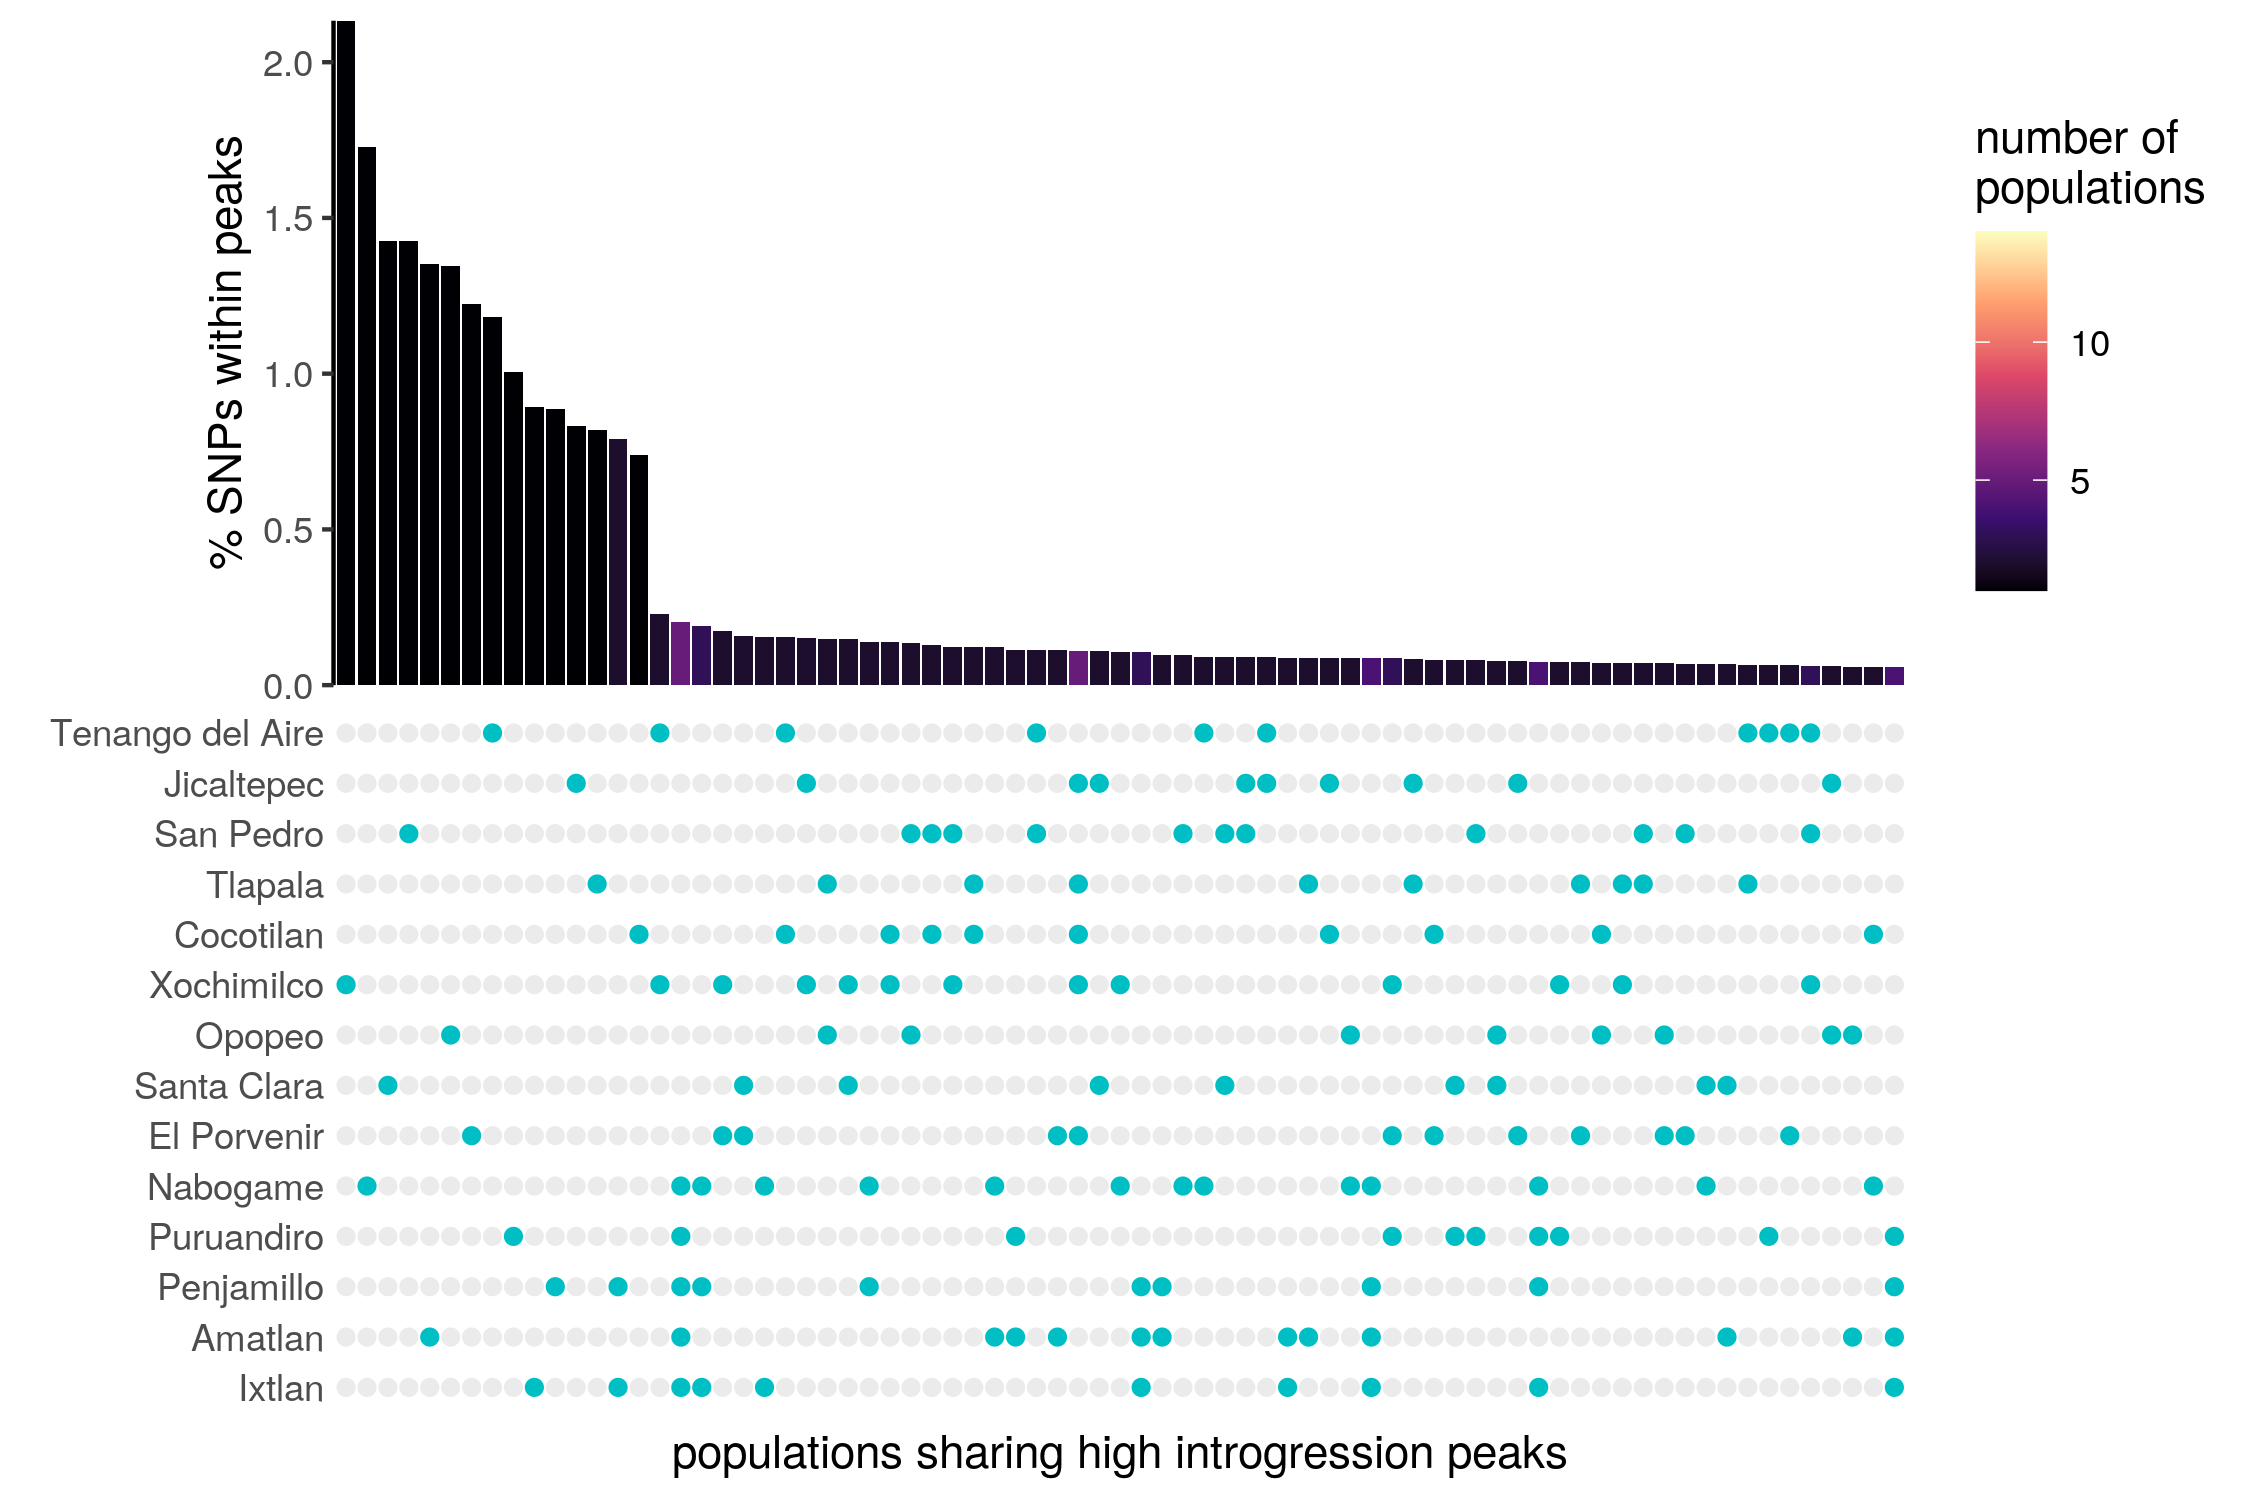
\includegraphics[width=\textwidth]{chapter2/figures/combmatrix_peak_sharing_mexicana.png}
\caption{\color{Gray} \textbf{High introgression peaks shared across sympatric \mexicana populations} Here we show the 75 most common combinations of populations that share ancestry peaks (introgressed ancestry $>$ 2 s.d. above each population's mean ancestry). Bar height represents the percent of SNPs genomewide within peaks shared by the populations highlighted in blue below. Populations are ordered from high (top) to low elevation.}
\label{combmatrix_peaks_mexicana}
\end{figure}

\begin{figure}[ht]
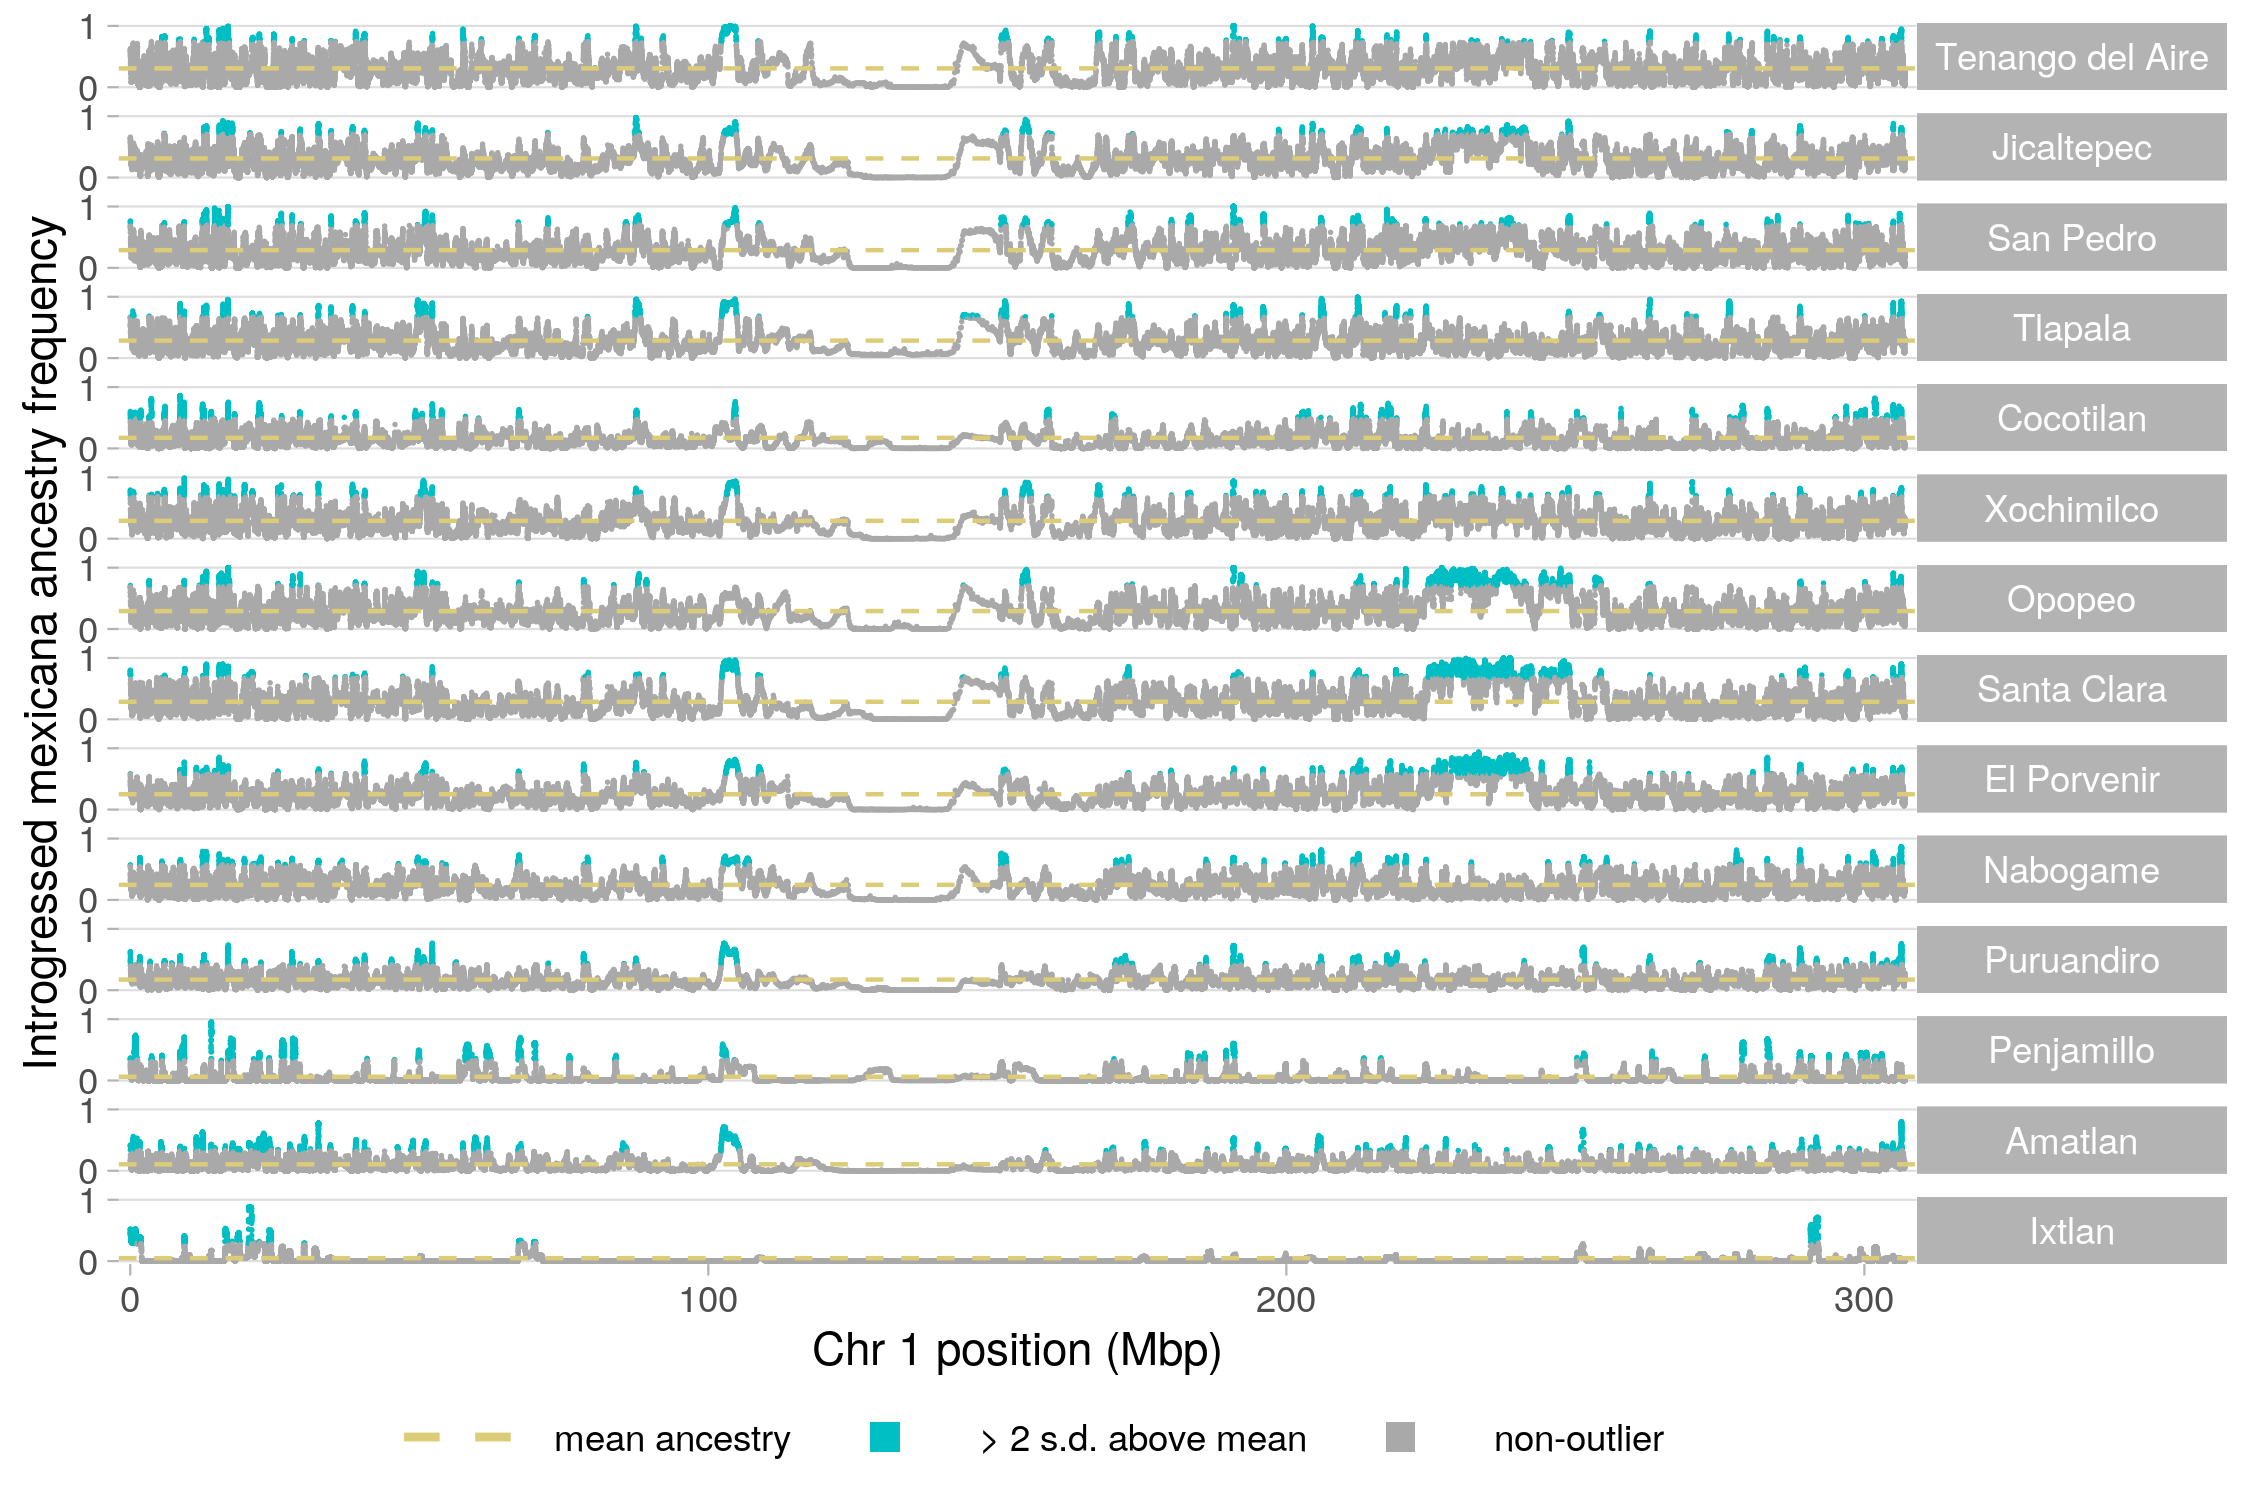
\includegraphics[width=.85\textwidth]{chapter2/figures/maize_shared_outliers_chr_1.png}
\caption{\color{Gray} \textbf{Introgression in maize landrace populations across chromosome 1}}
\label{maize_chr1}
\end{figure}

\begin{figure}[ht]
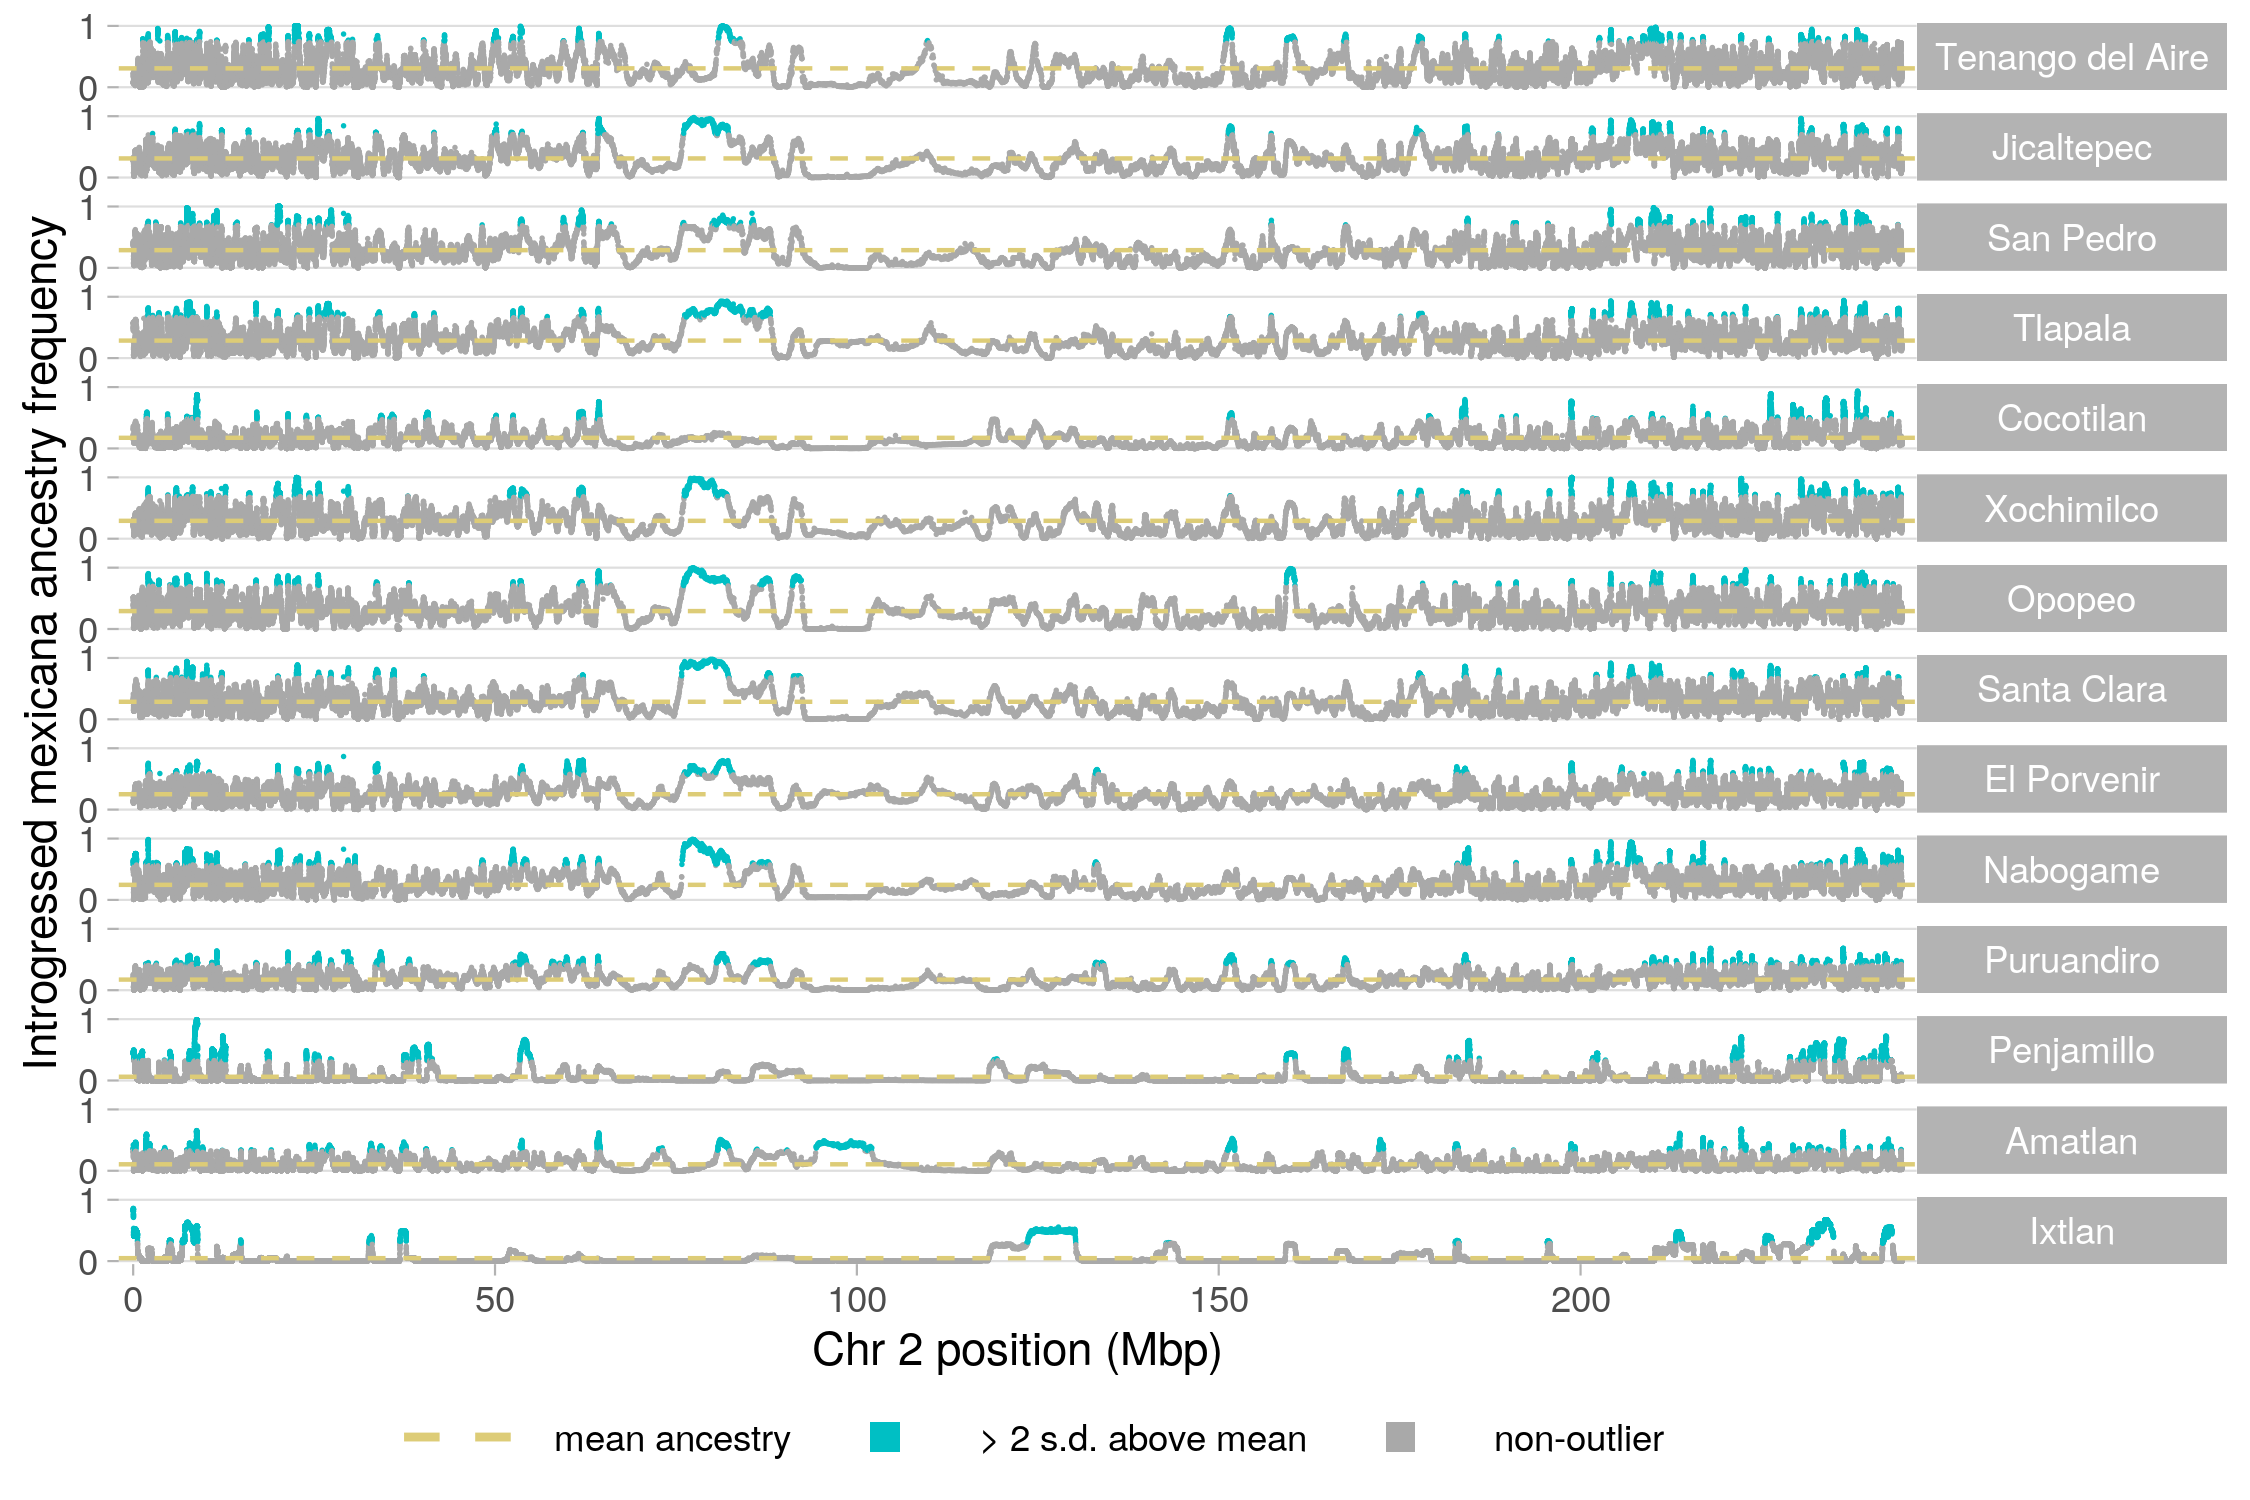
\includegraphics[width=.85\textwidth]{chapter2/figures/maize_shared_outliers_chr_2.png}
\caption{\color{Gray} \textbf{Introgression in maize landrace populations across chromosome 2}}
\label{maize_chr2}
\end{figure}

\begin{figure}[ht]
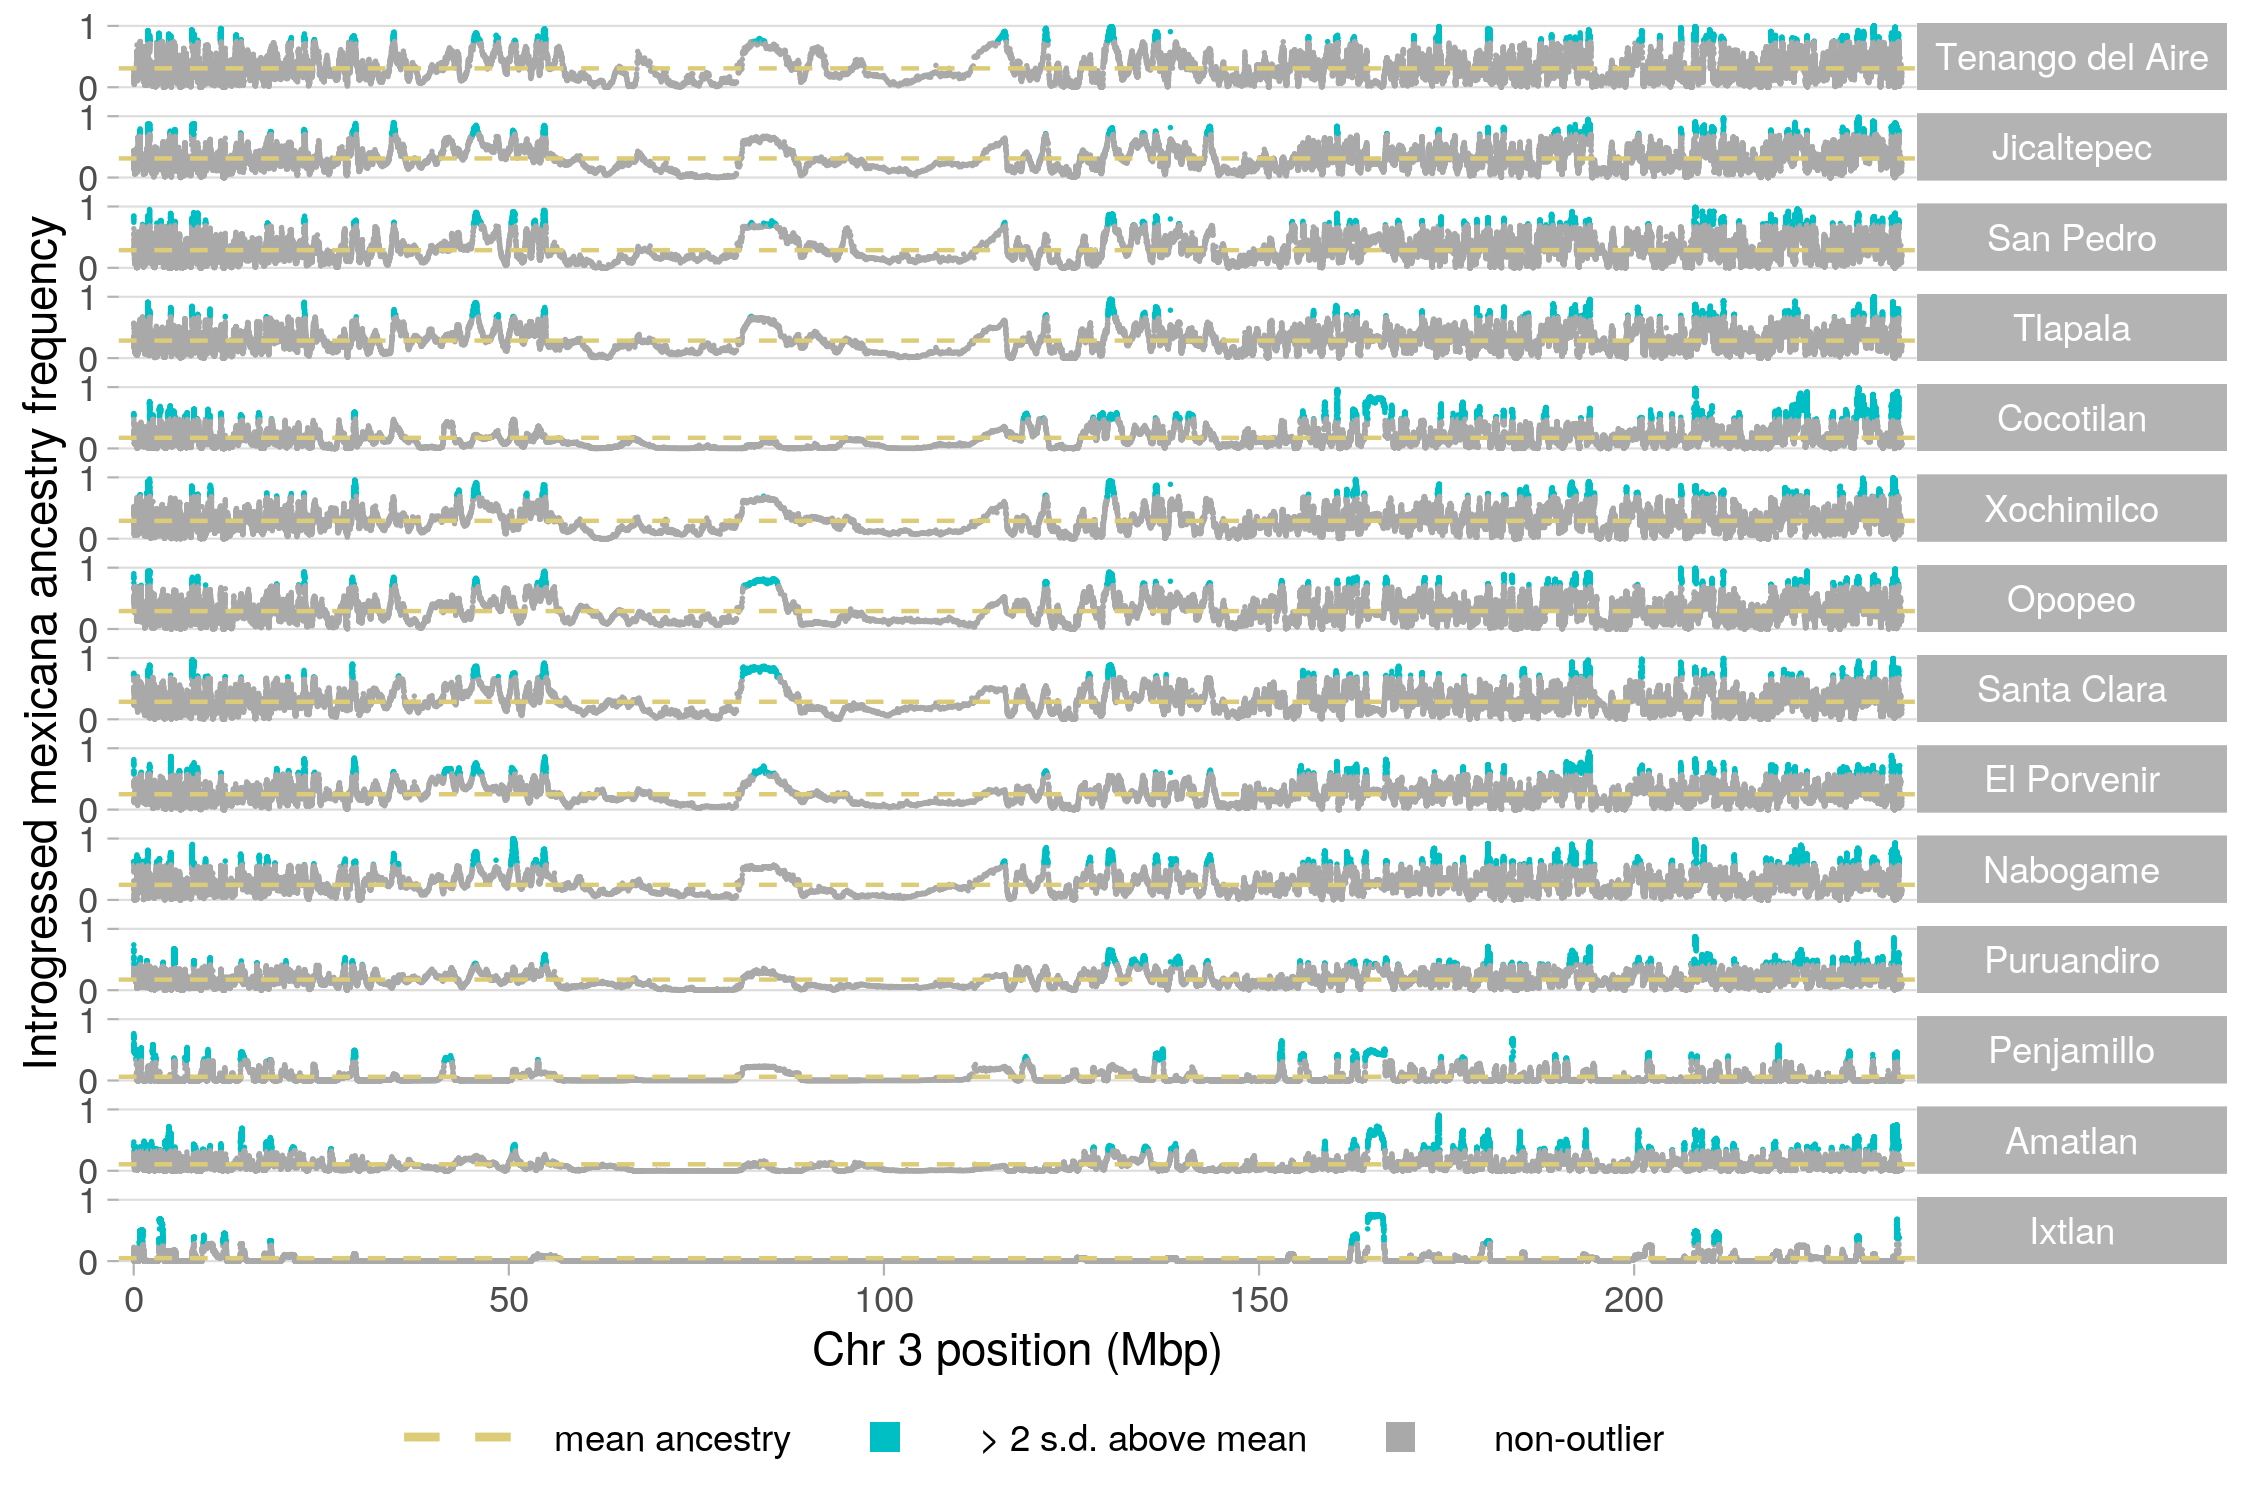
\includegraphics[width=.85\textwidth]{chapter2/figures/maize_shared_outliers_chr_3.png}
\caption{\color{Gray} \textbf{Introgression in maize landrace populations across chromosome 3}}
\label{maize_chr3}
\end{figure}

\begin{figure}[ht]
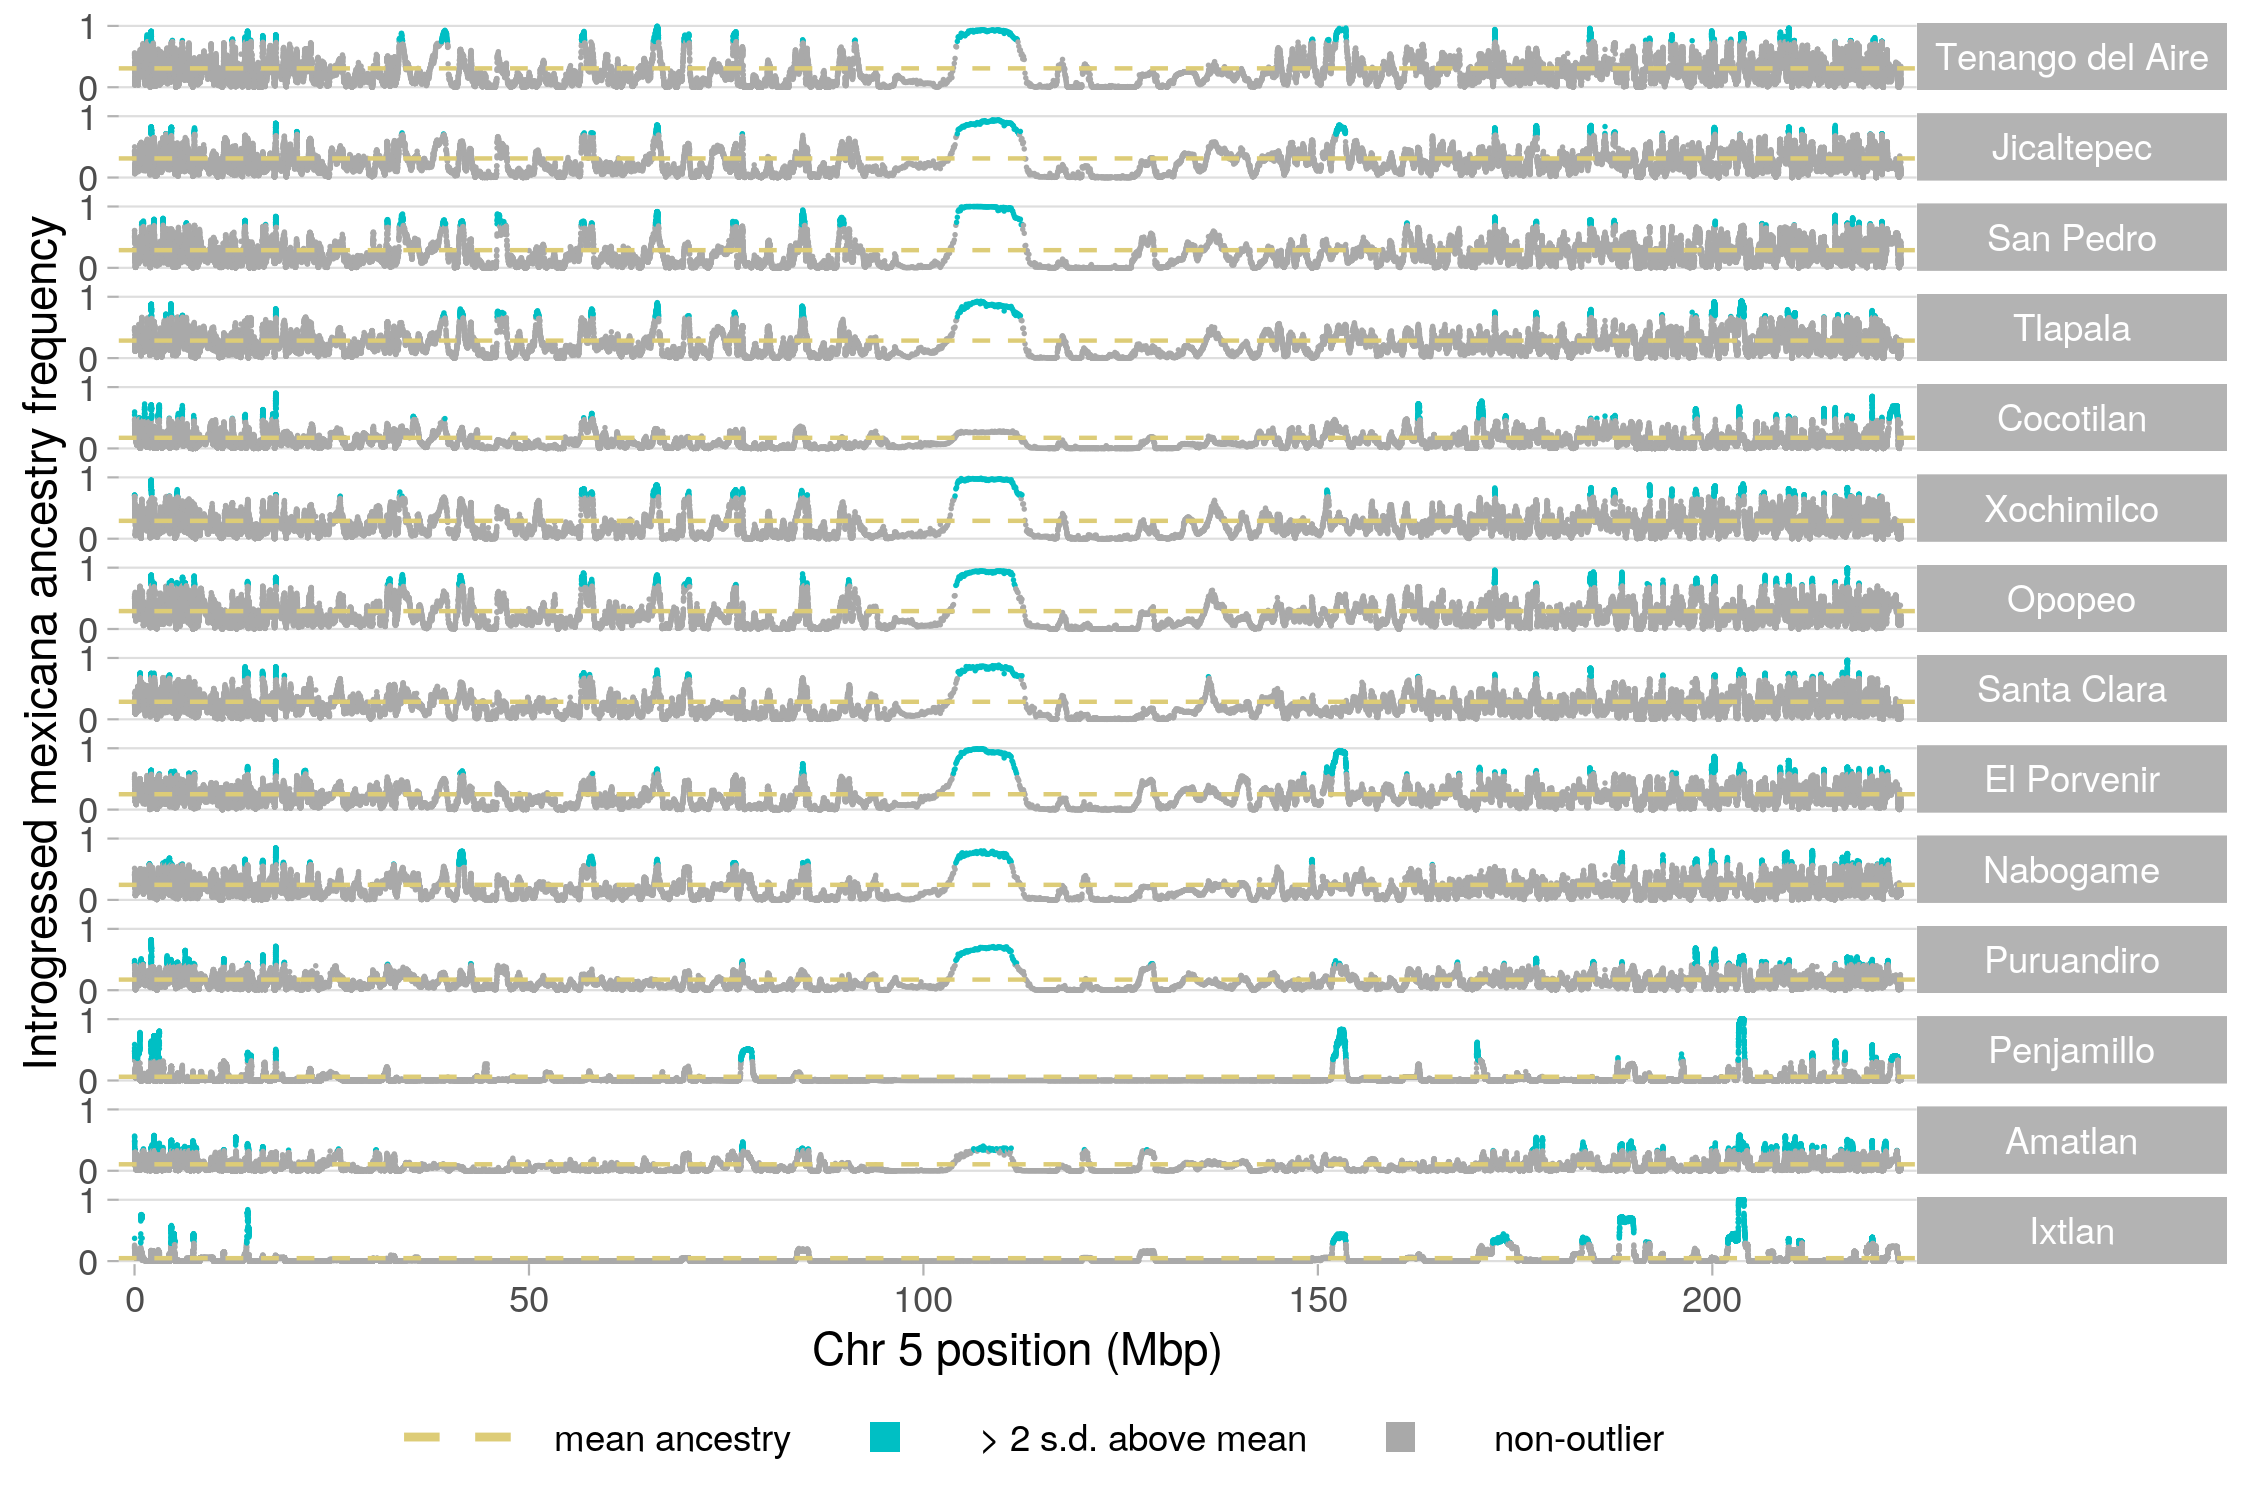
\includegraphics[width=.85\textwidth]{chapter2/figures/maize_shared_outliers_chr_5.png}
\caption{\color{Gray} \textbf{Introgression in maize landrace populations across chromosome 5}}
\label{maize_chr5}
\end{figure}

\begin{figure}[ht]
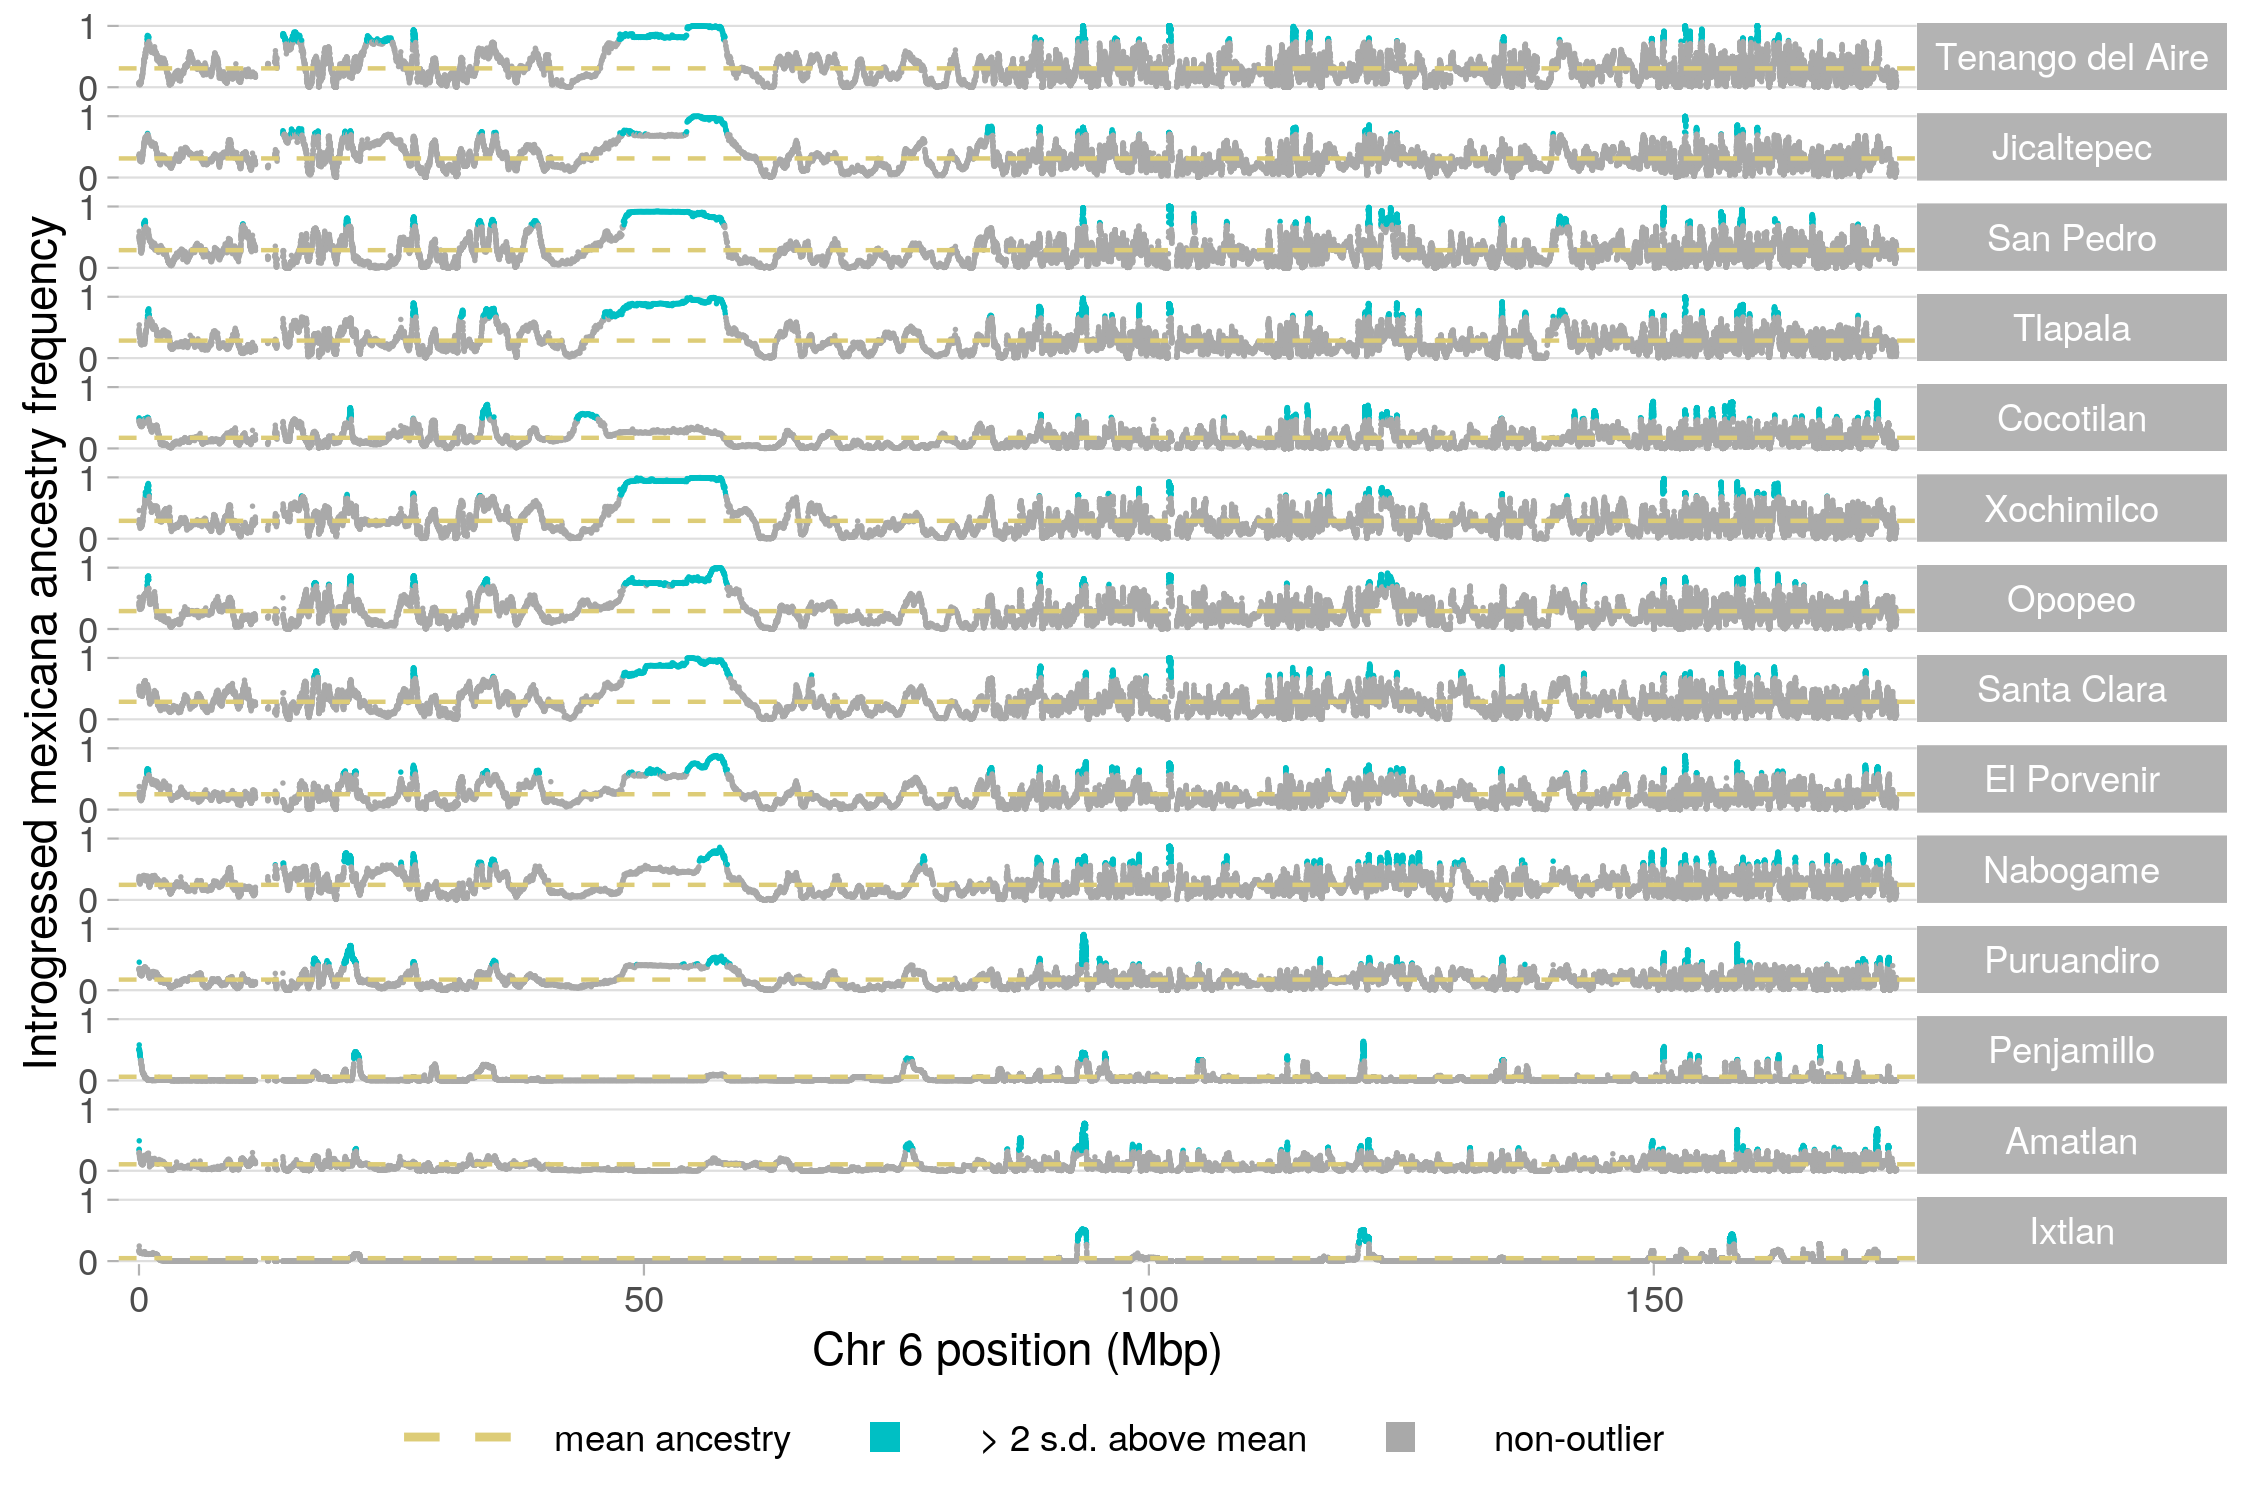
\includegraphics[width=.85\textwidth]{chapter2/figures/maize_shared_outliers_chr_6.png}
\caption{\color{Gray} \textbf{Introgression in maize landrace populations across chromosome 6}}
\label{maize_chr6}
\end{figure}

\begin{figure}[ht]
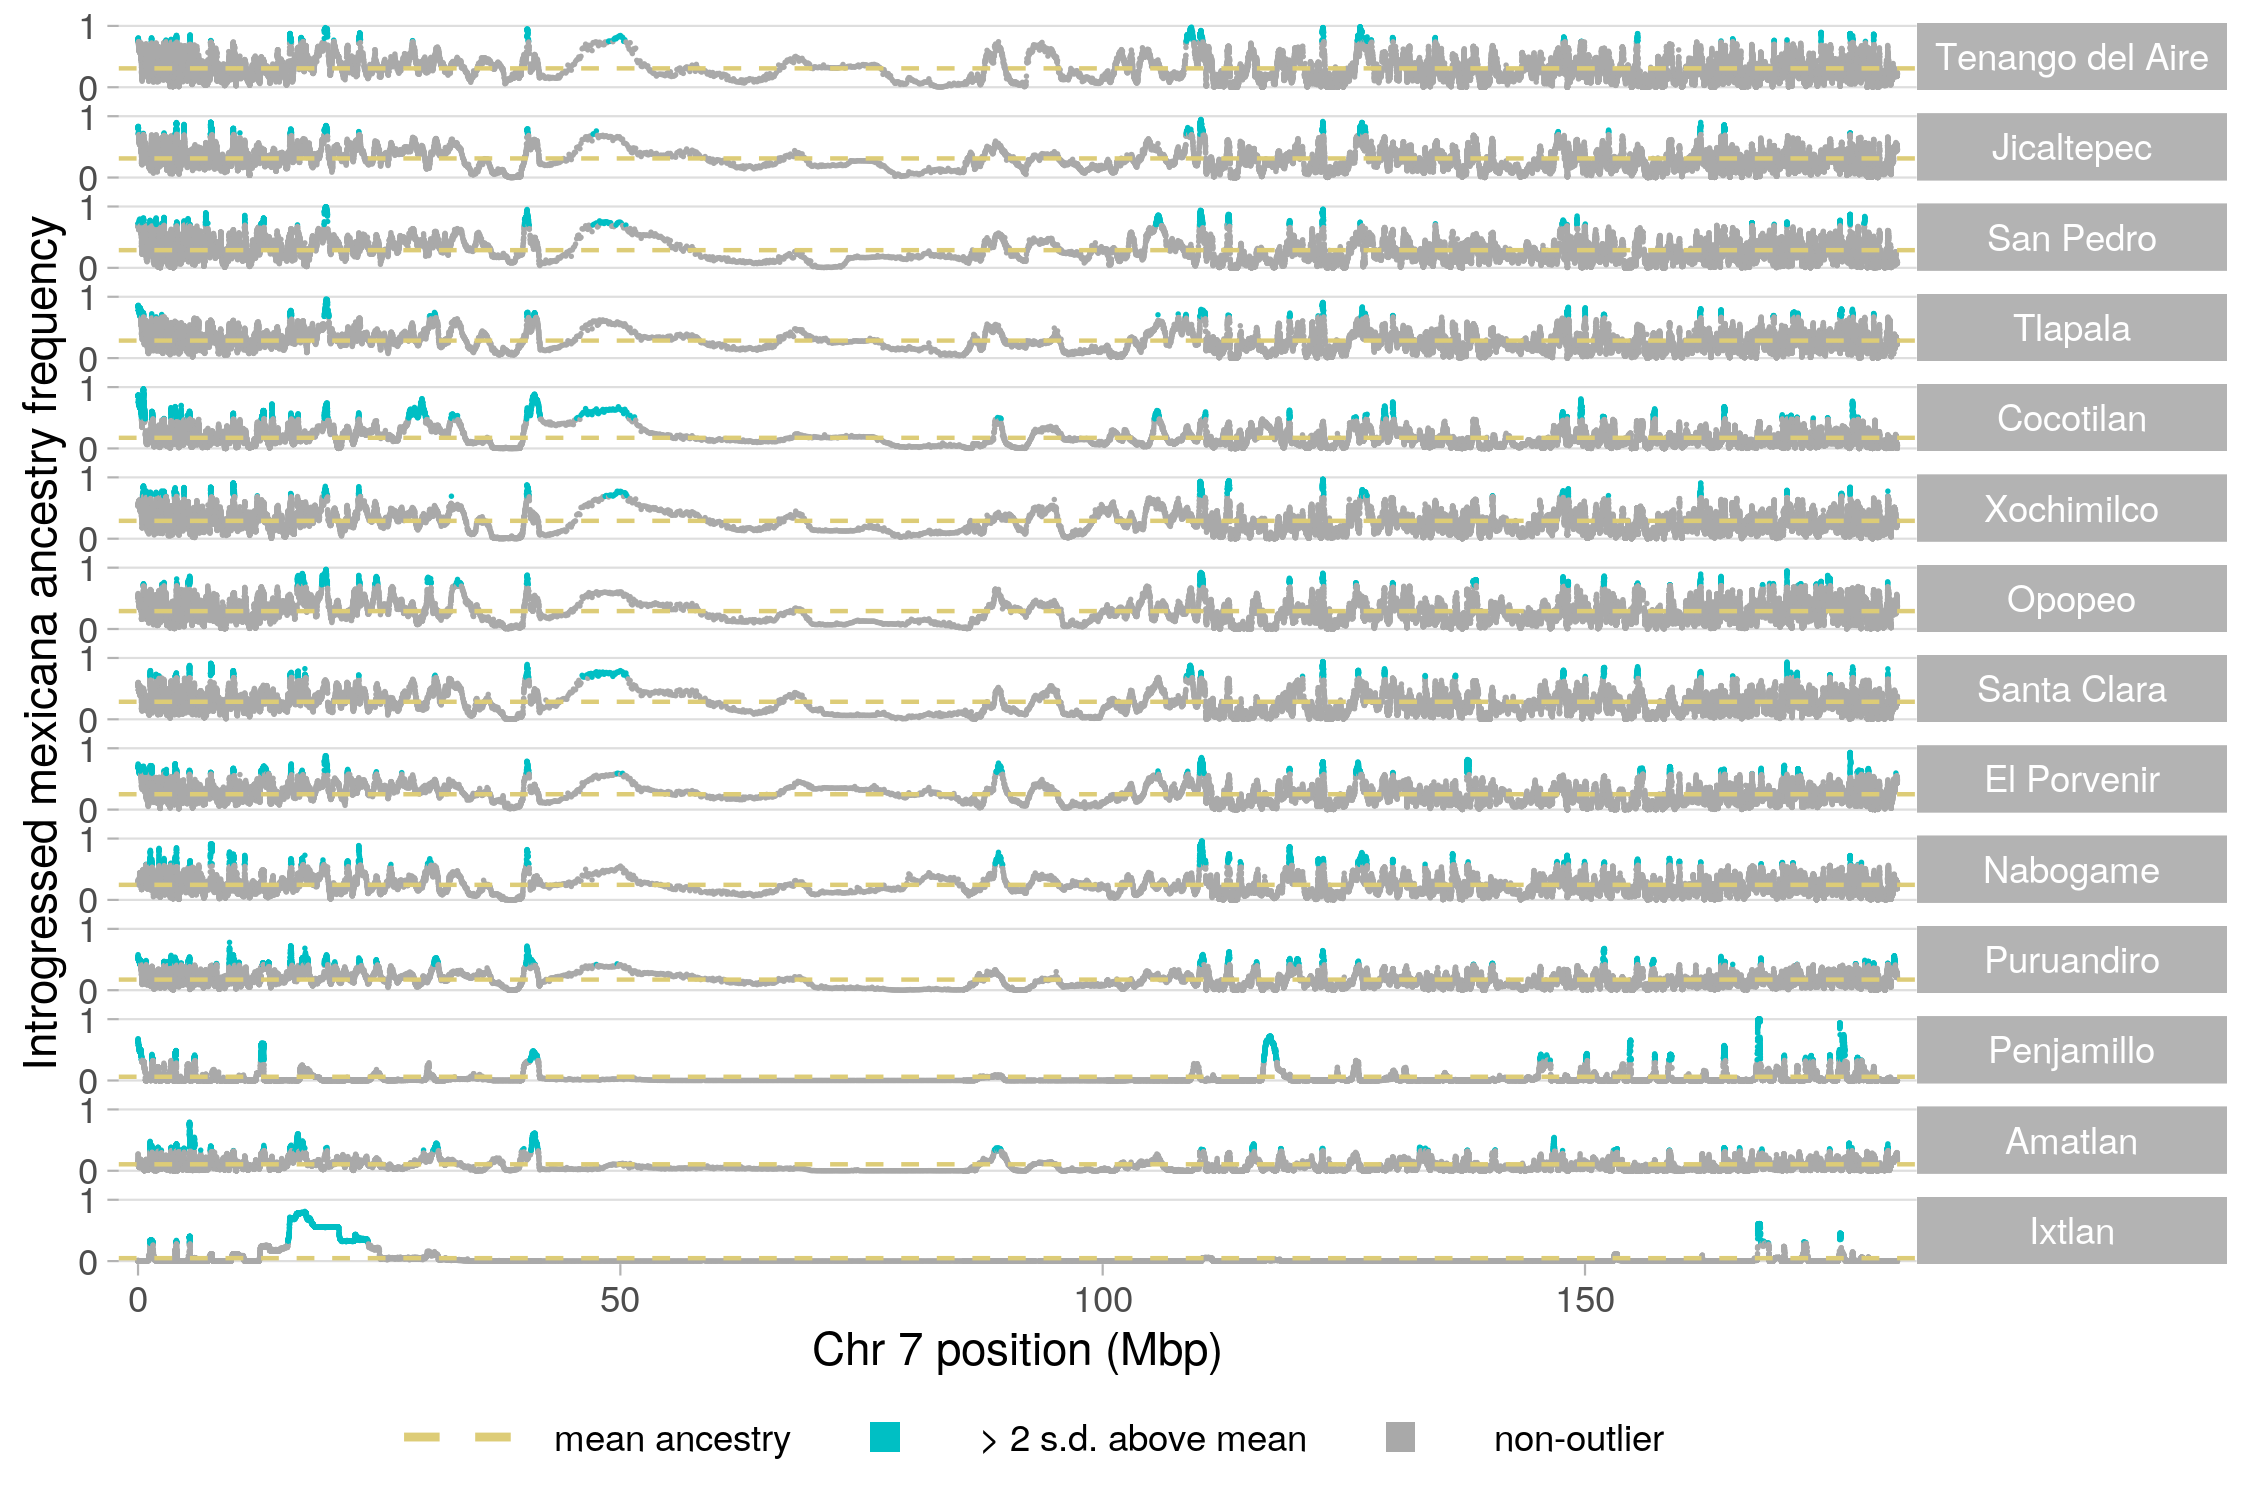
\includegraphics[width=.85\textwidth]{chapter2/figures/maize_shared_outliers_chr_7.png}
\caption{\color{Gray} \textbf{Introgression in maize landrace populations across chromosome 7}}
\label{maize_chr7}
\end{figure}

\begin{figure}[ht]
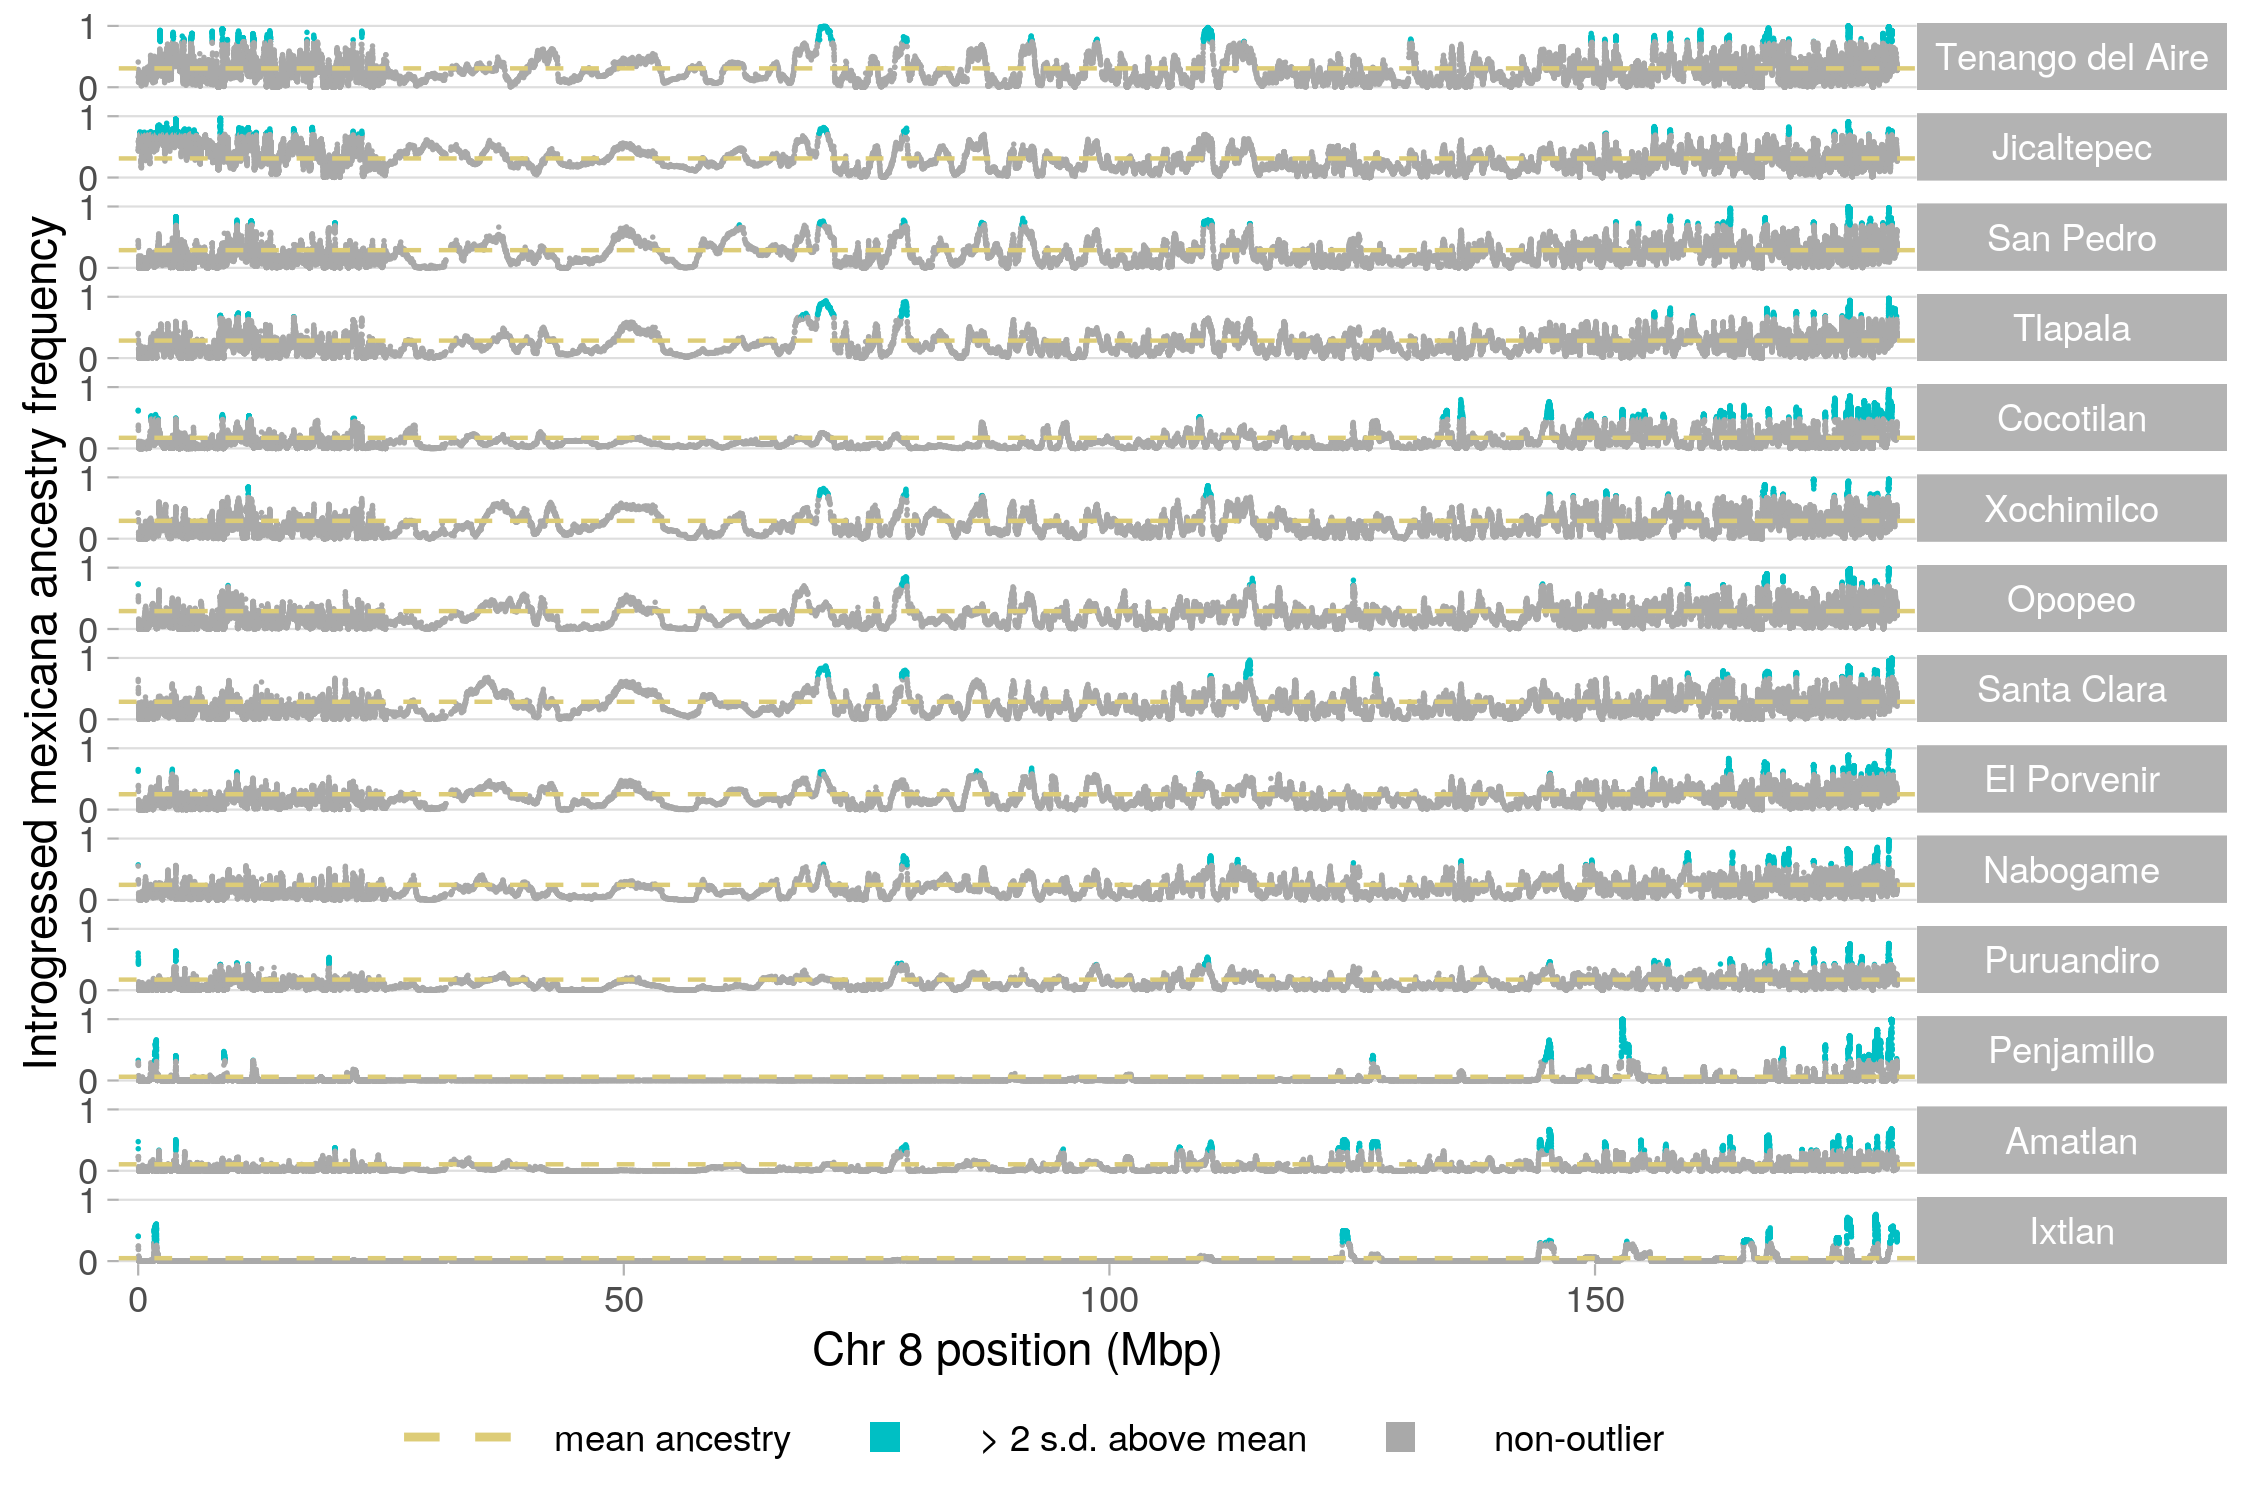
\includegraphics[width=.85\textwidth]{chapter2/figures/maize_shared_outliers_chr_8.png}
\caption{\color{Gray} \textbf{Introgression in maize landrace populations across chromosome 8}}
\label{maize_chr8}
\end{figure}

\begin{figure}[ht]
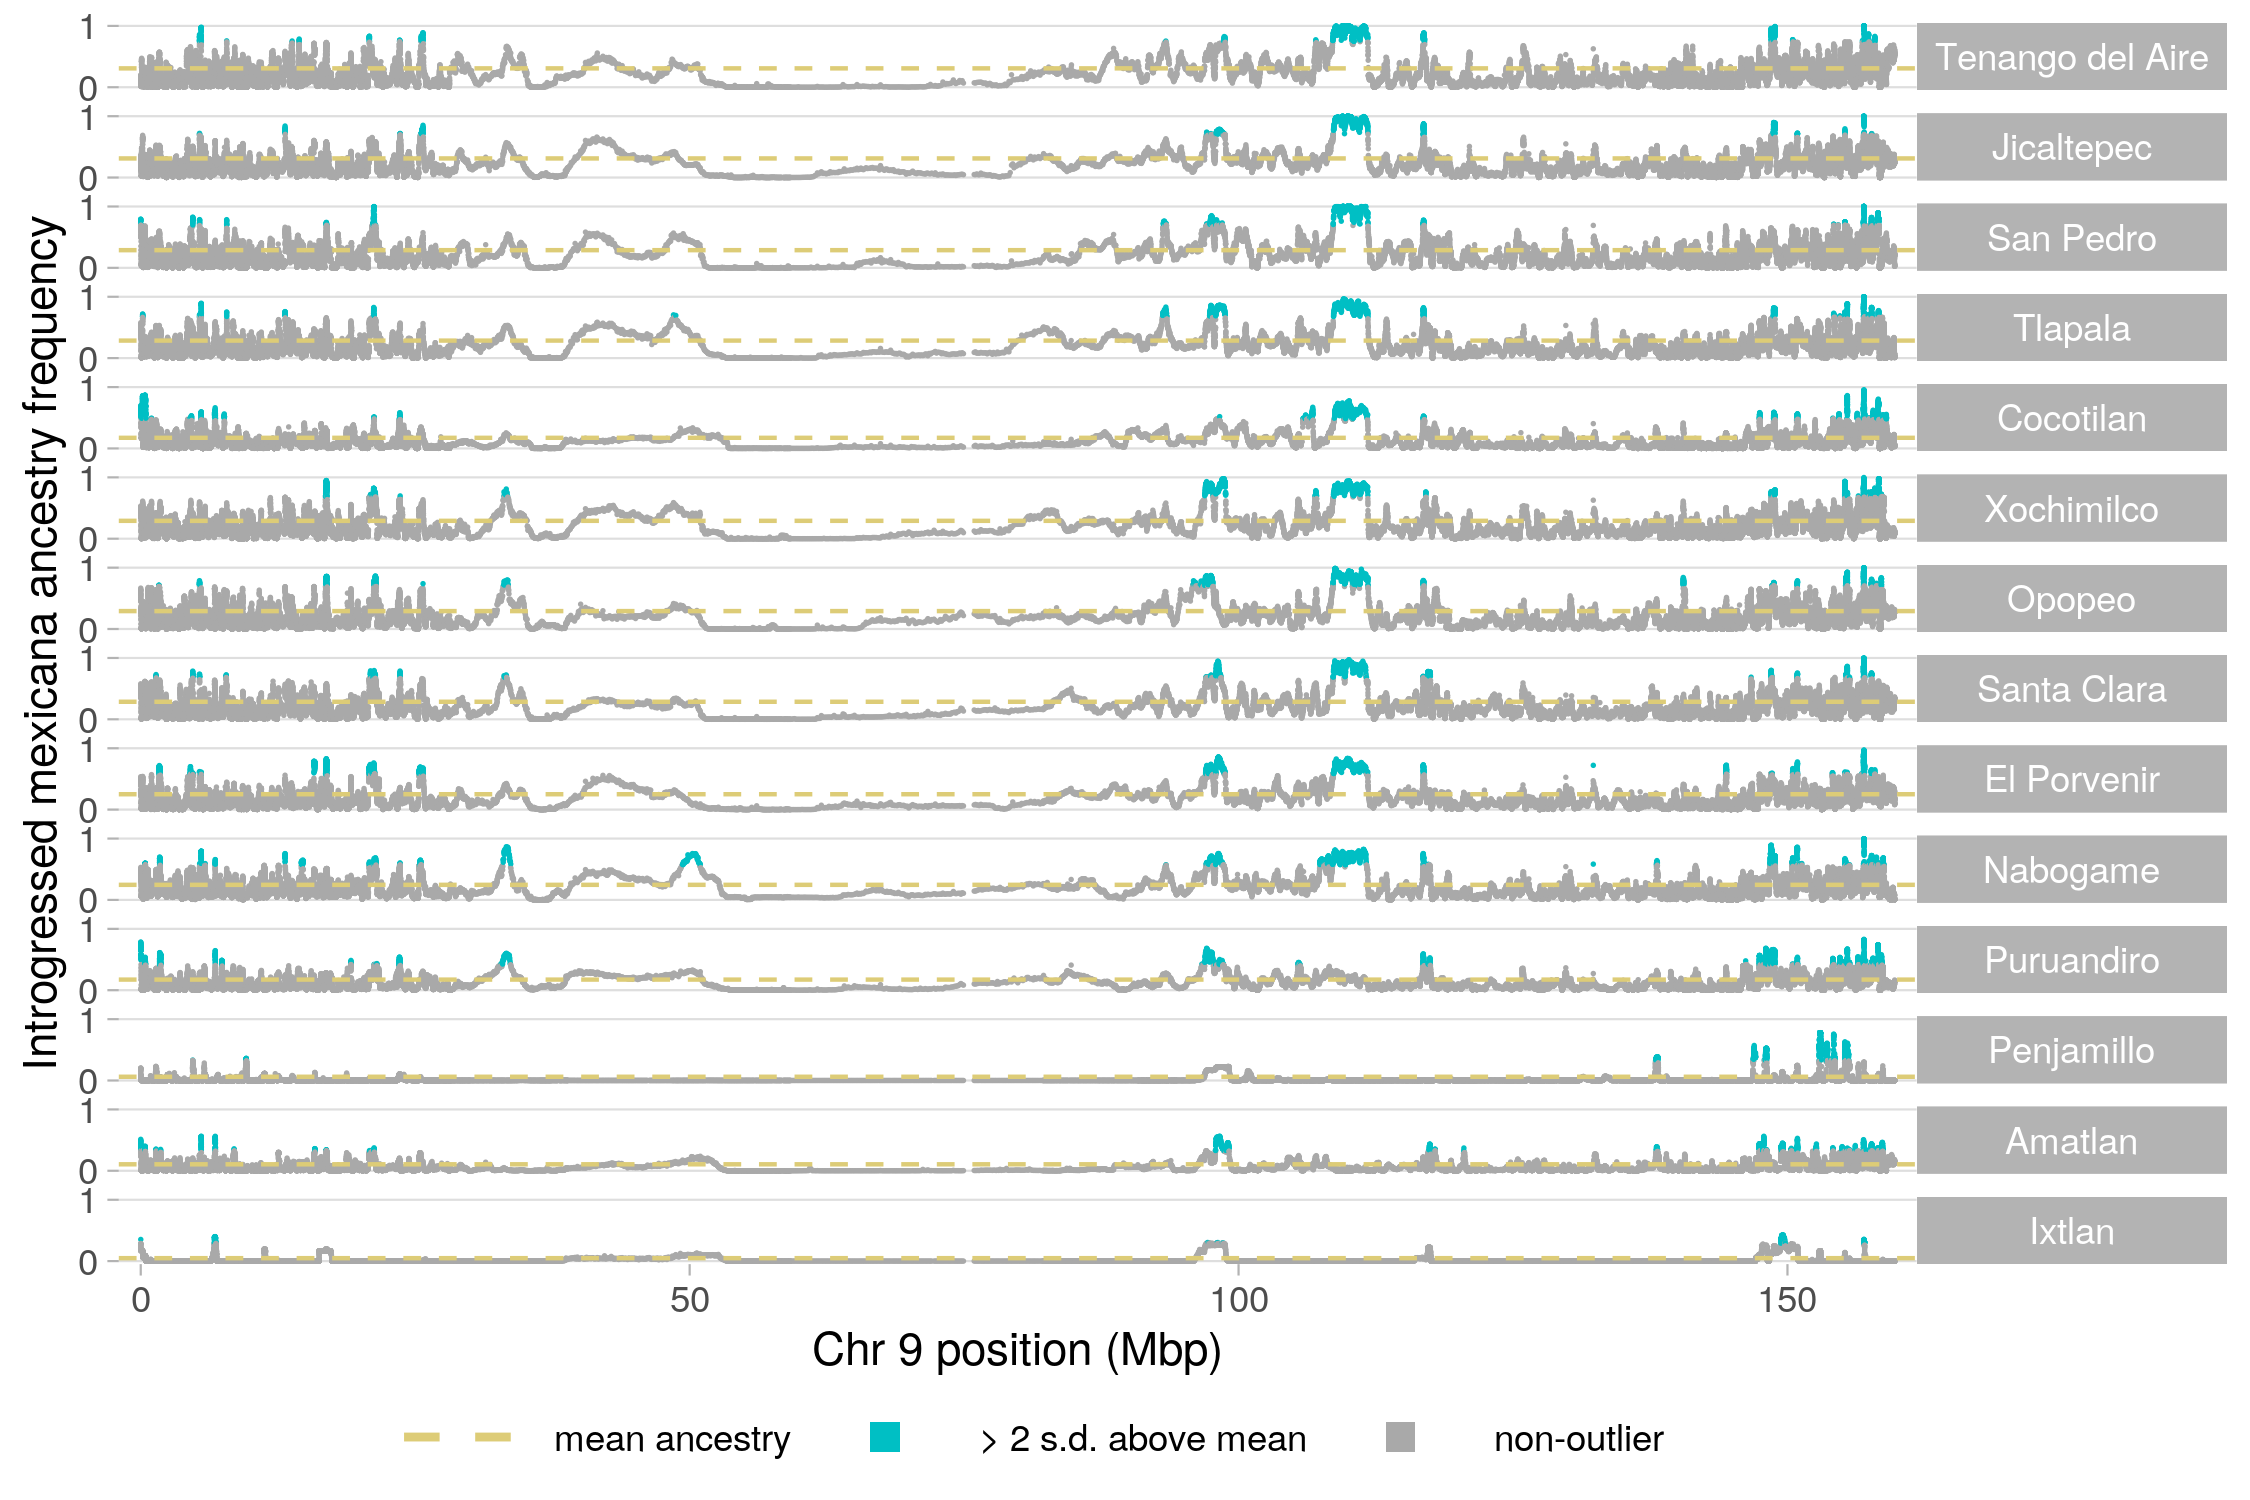
\includegraphics[width=.85\textwidth]{chapter2/figures/maize_shared_outliers_chr_9.png}
\caption{\color{Gray} \textbf{Introgression in maize landrace populations across chromosome 9}}
\label{maize_chr9}
\end{figure}

\begin{figure}[ht]
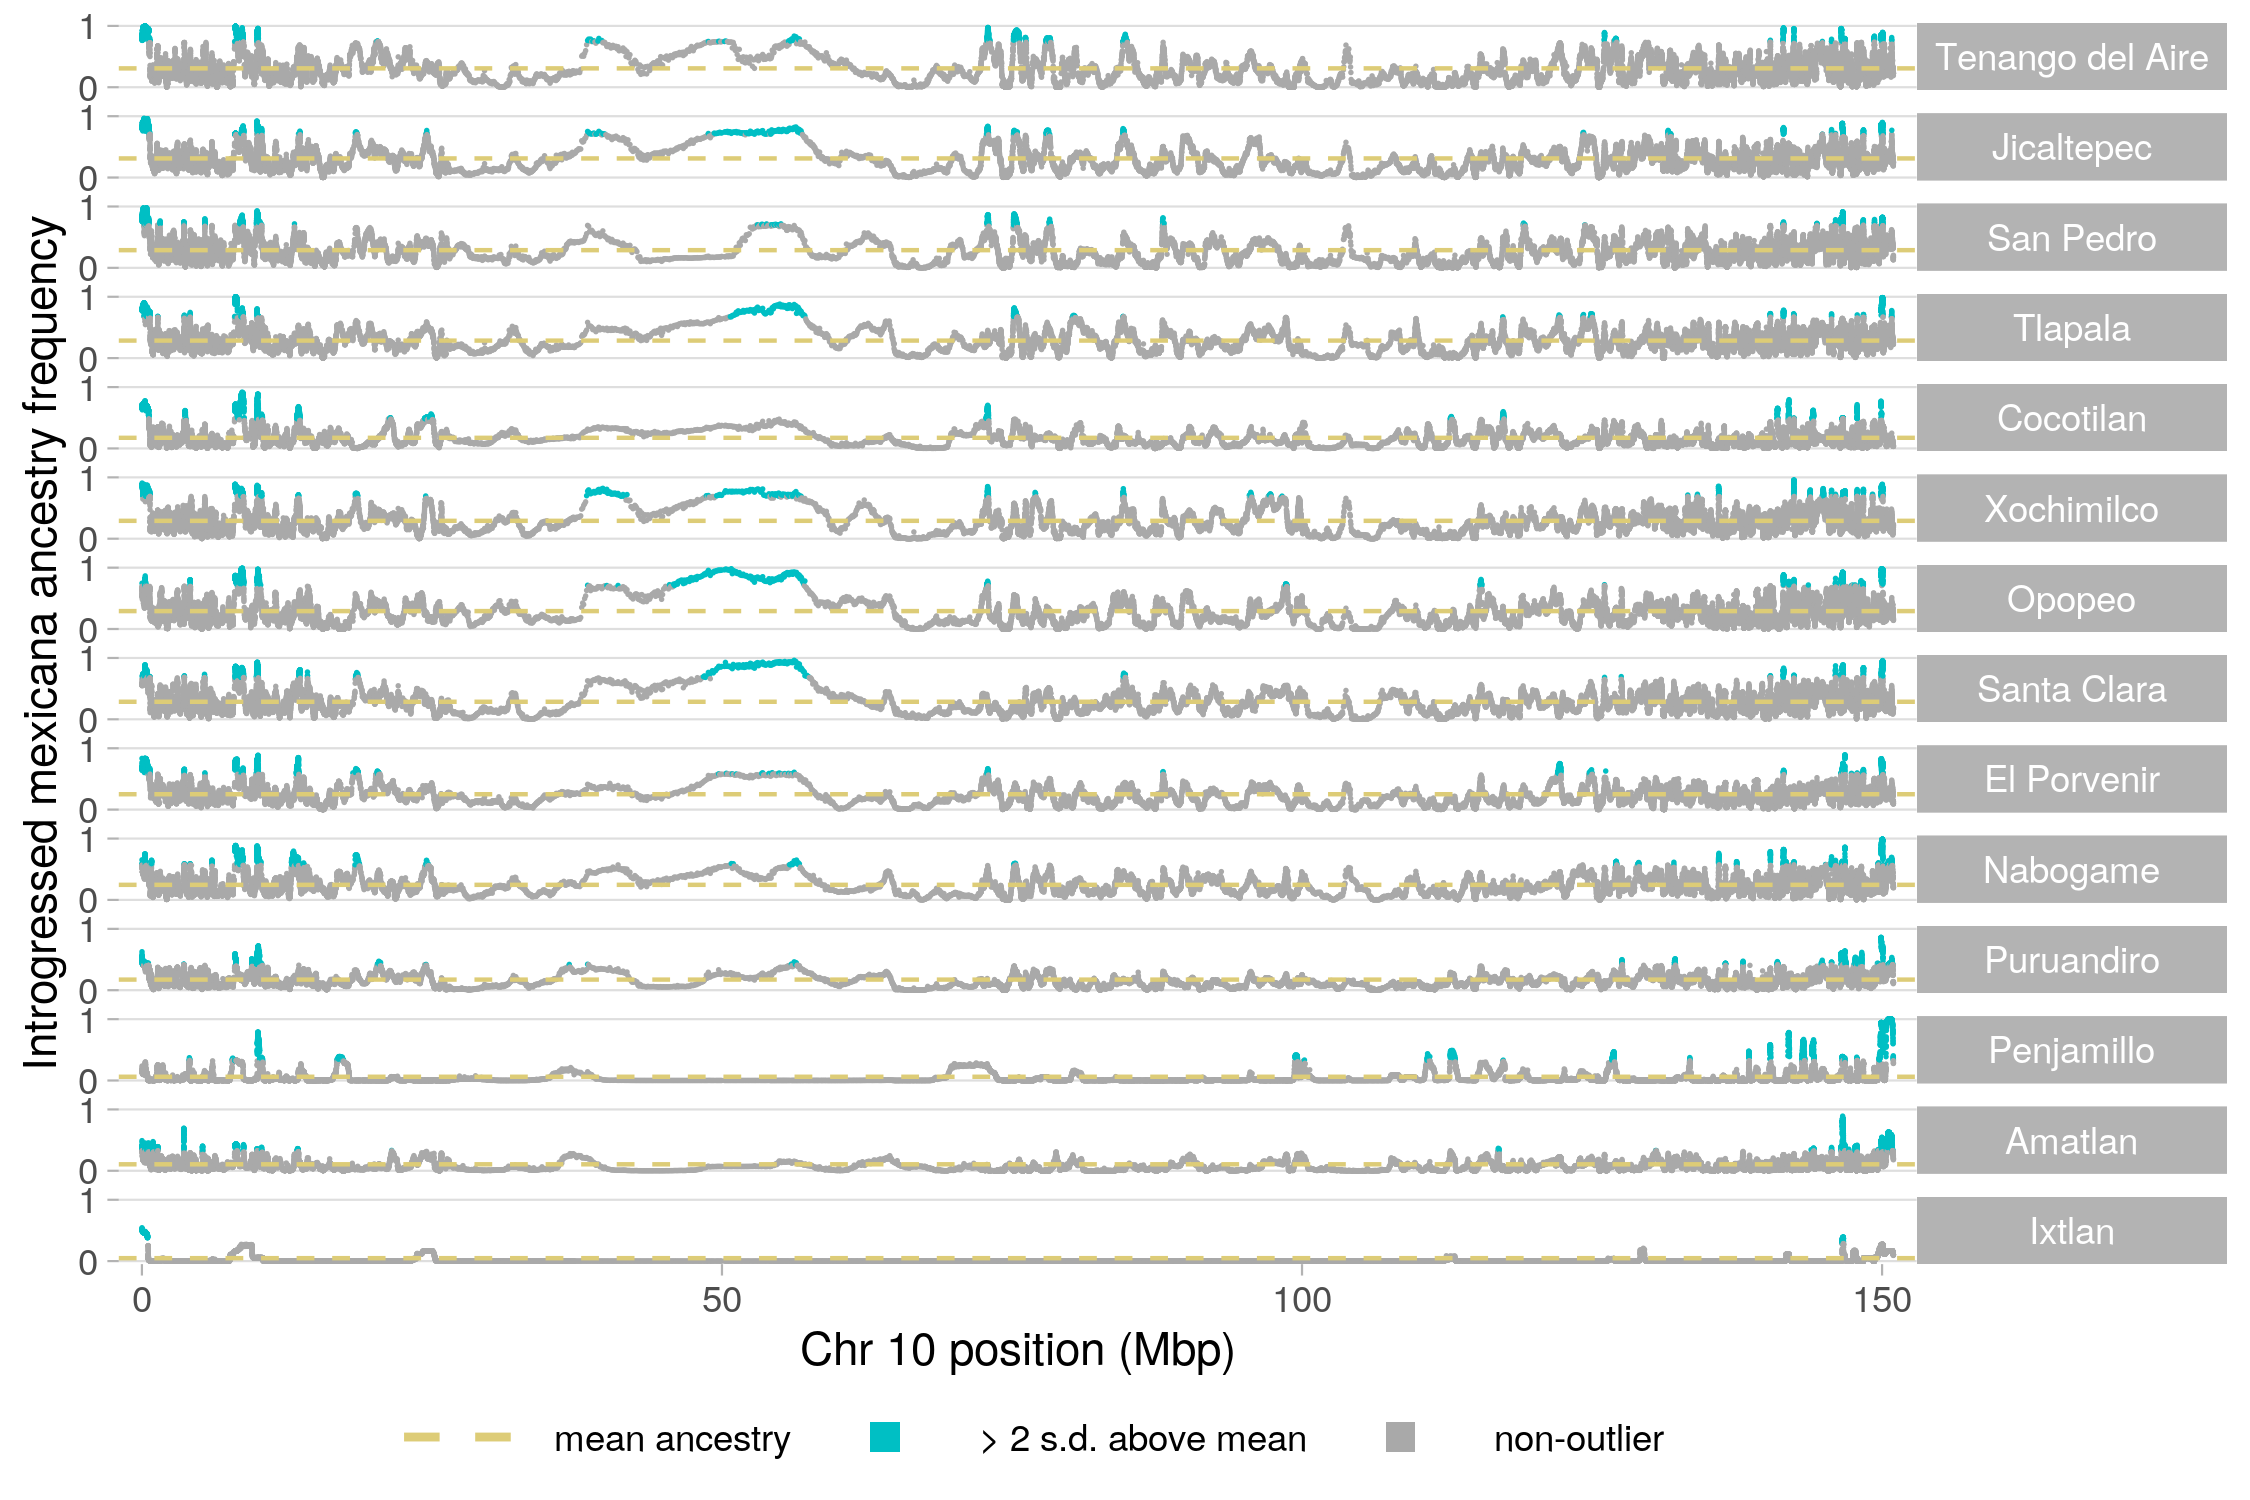
\includegraphics[width=.85\textwidth]{chapter2/figures/maize_shared_outliers_chr_10.png}
\caption{\color{Gray} \textbf{Introgression in maize landrace populations across chromosome 10}}
\label{maize_chr10}
\end{figure}

\begin{figure}[ht]
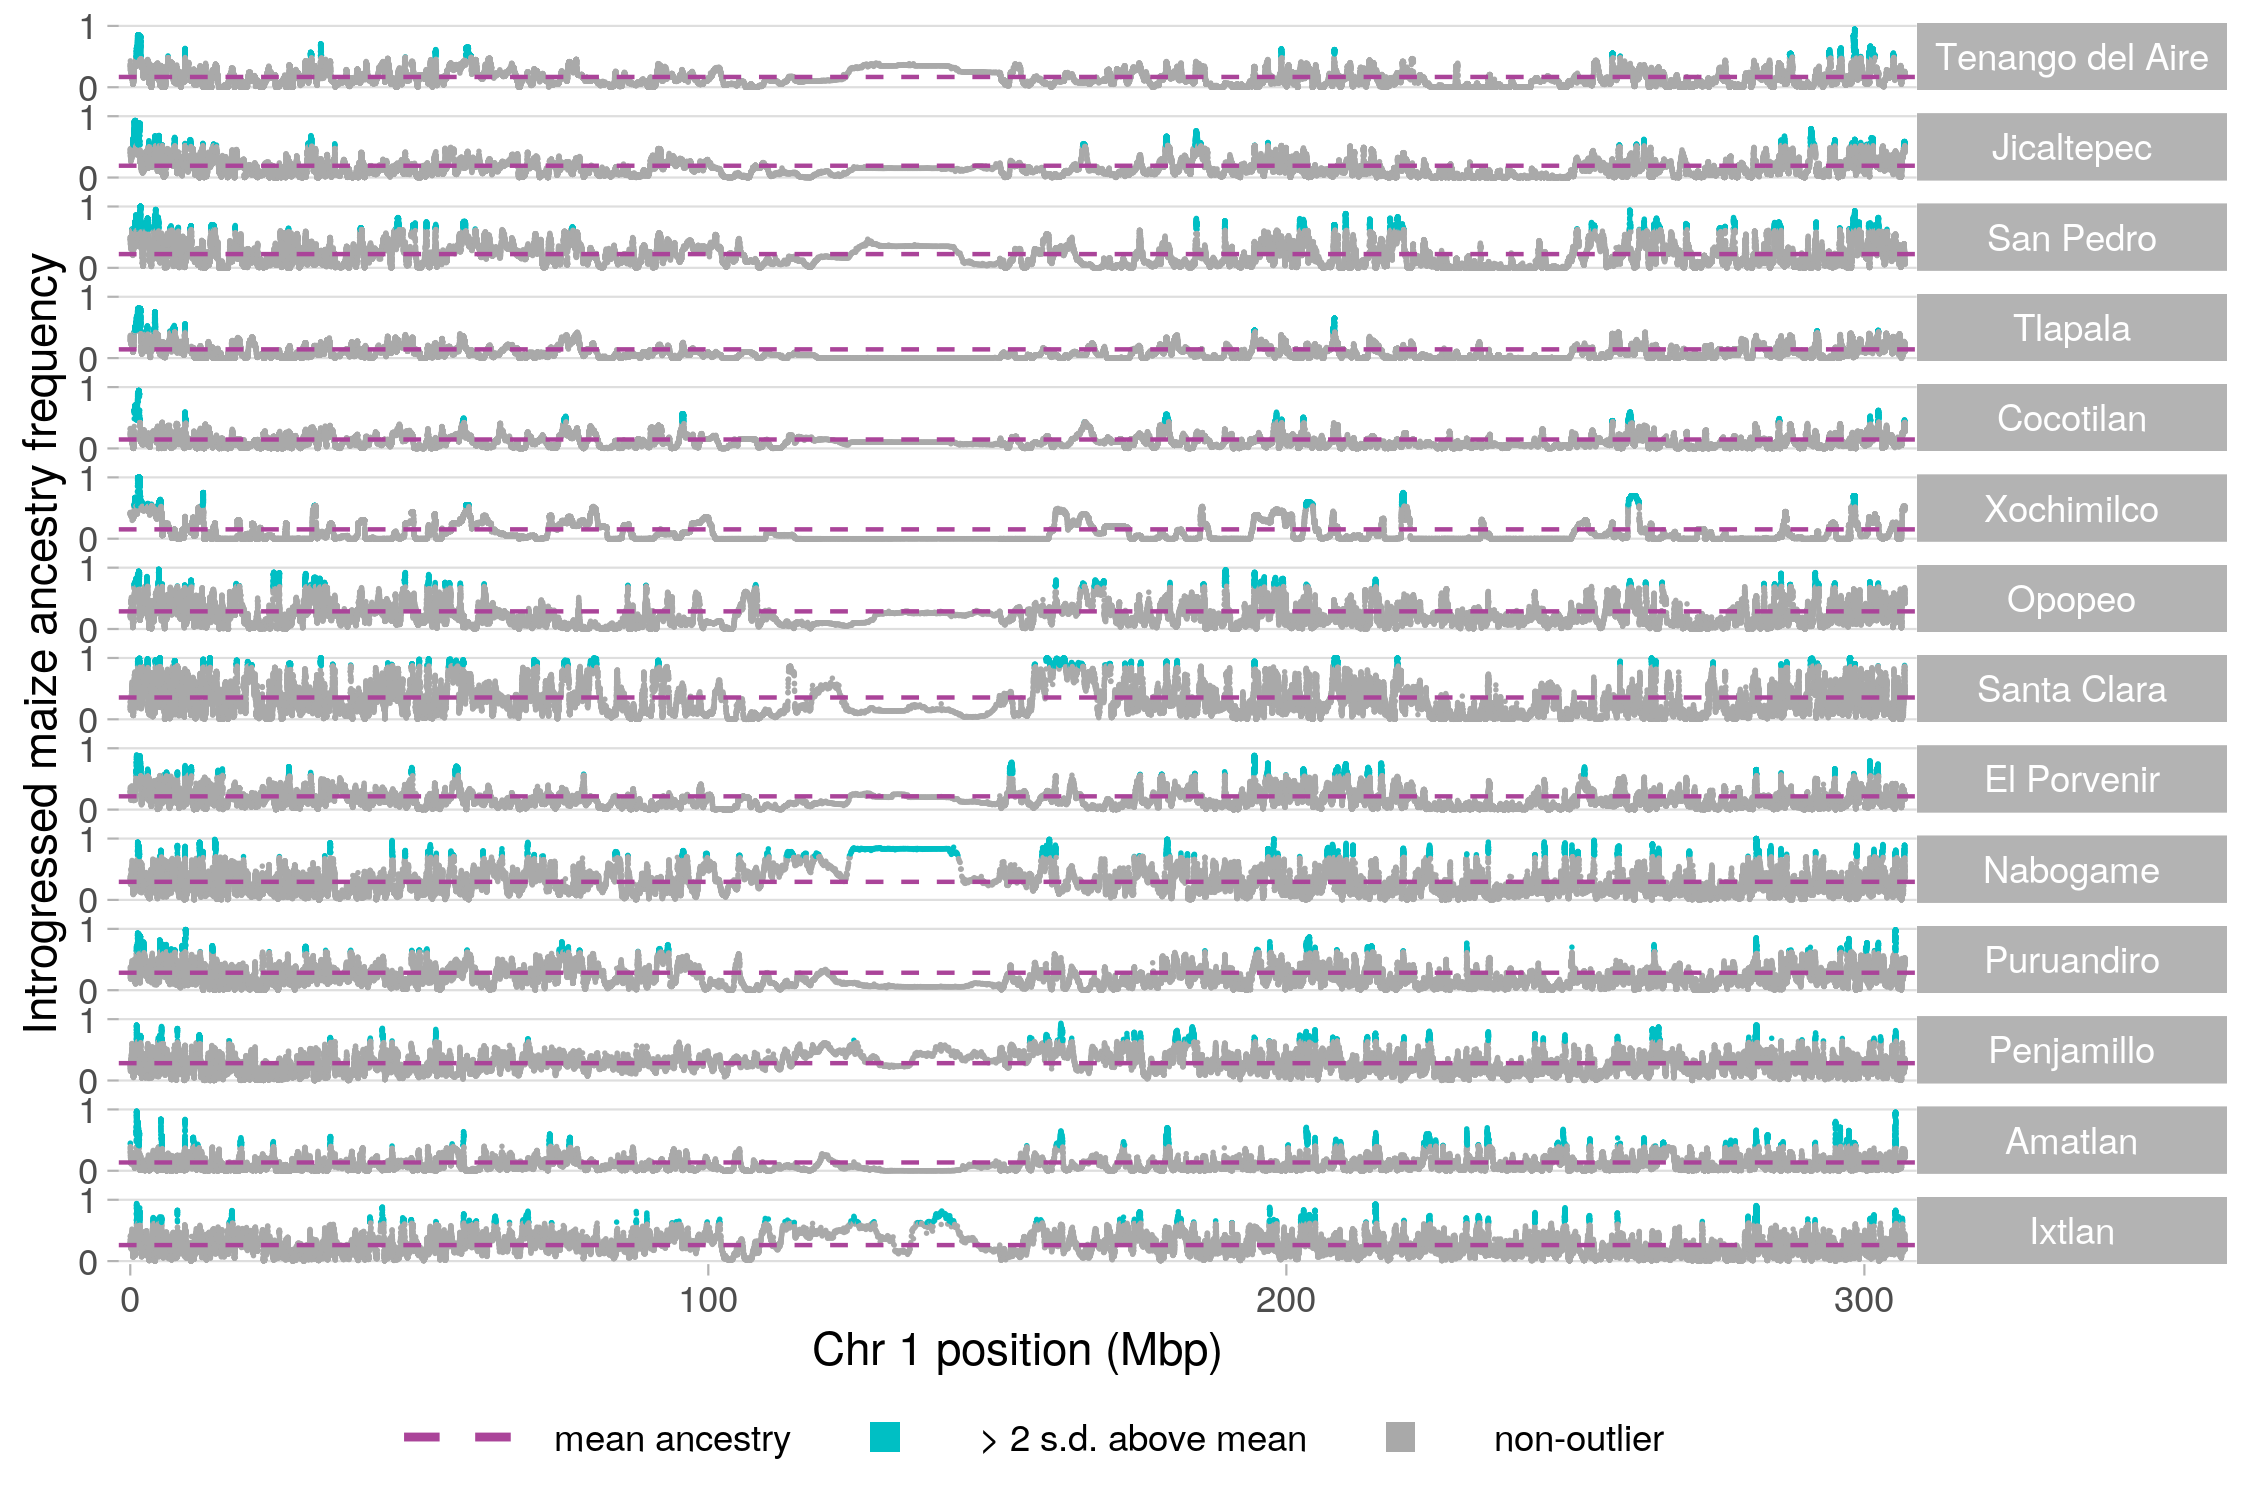
\includegraphics[width=.85\textwidth]{chapter2/figures/mexicana_shared_outliers_chr_1.png}
\caption{\color{Gray} \textbf{Introgression in \mexicana populations across chromosome 1}}
\label{mexicana_chr1}
\end{figure}

\begin{figure}[ht]
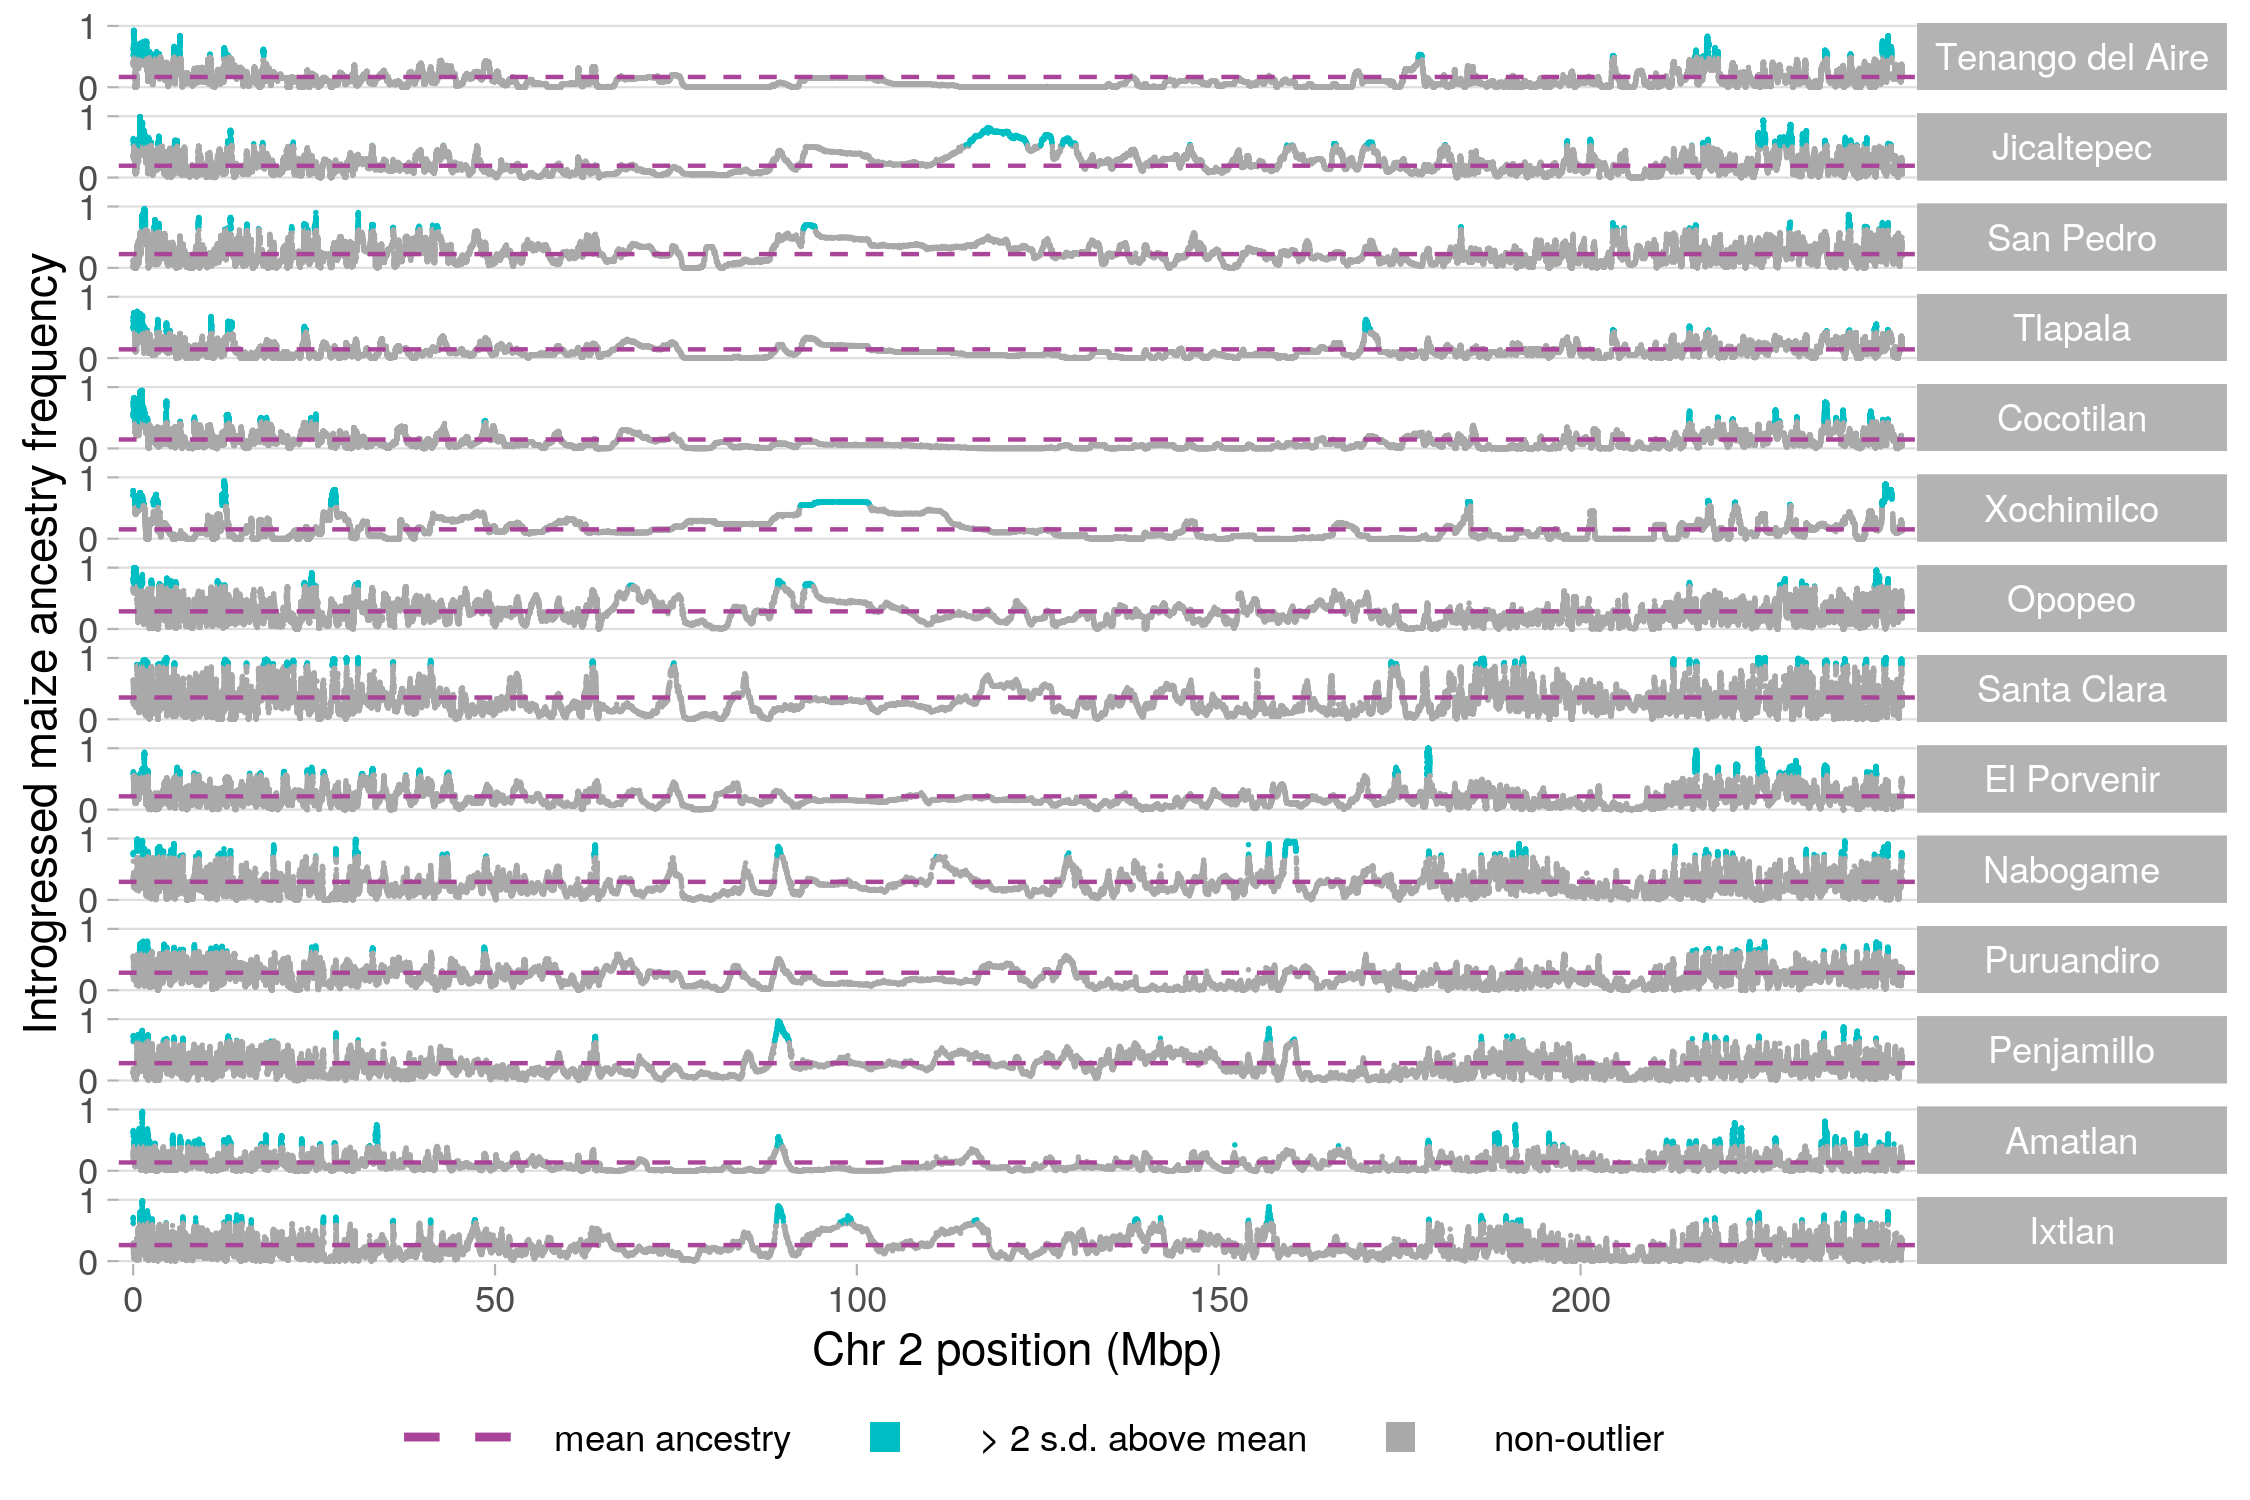
\includegraphics[width=.85\textwidth]{chapter2/figures/mexicana_shared_outliers_chr_2.png}
\caption{\color{Gray} \textbf{Introgression in \mexicana populations across chromosome 2}}
\label{mexicana_chr2}
\end{figure}

\begin{figure}[ht]
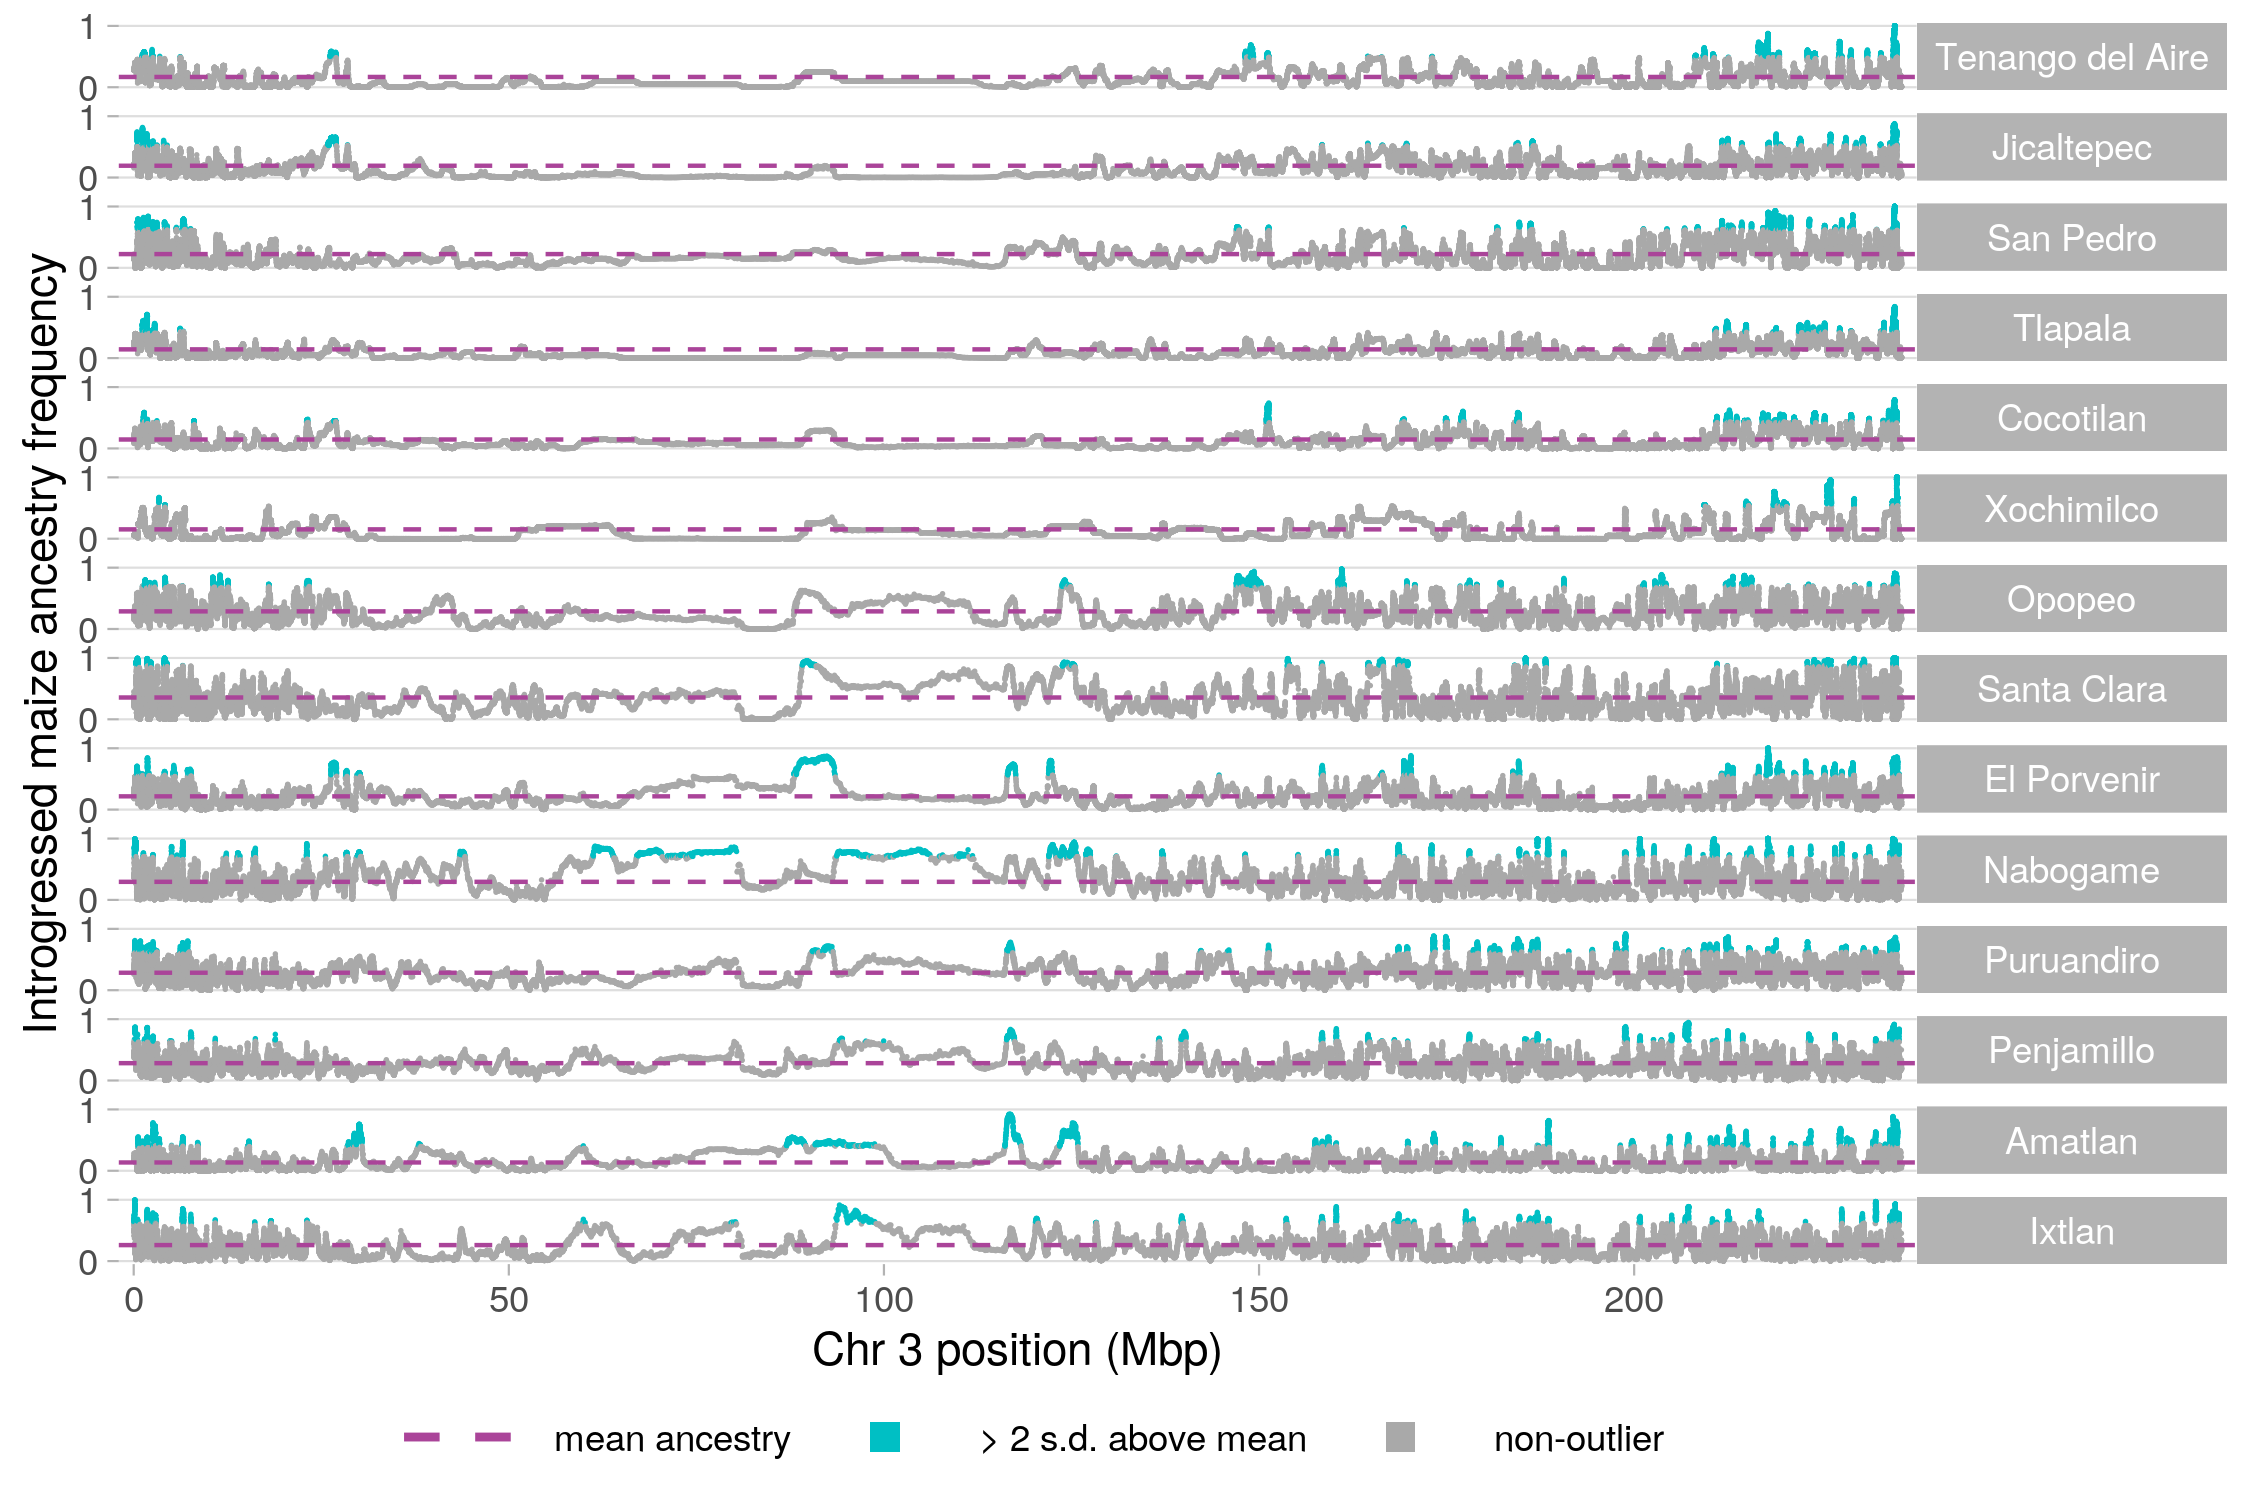
\includegraphics[width=.85\textwidth]{chapter2/figures/mexicana_shared_outliers_chr_3.png}
\caption{\color{Gray} \textbf{Introgression in \mexicana populations across chromosome 3}}
\label{mexicana_chr3}
\end{figure}

\begin{figure}[ht]
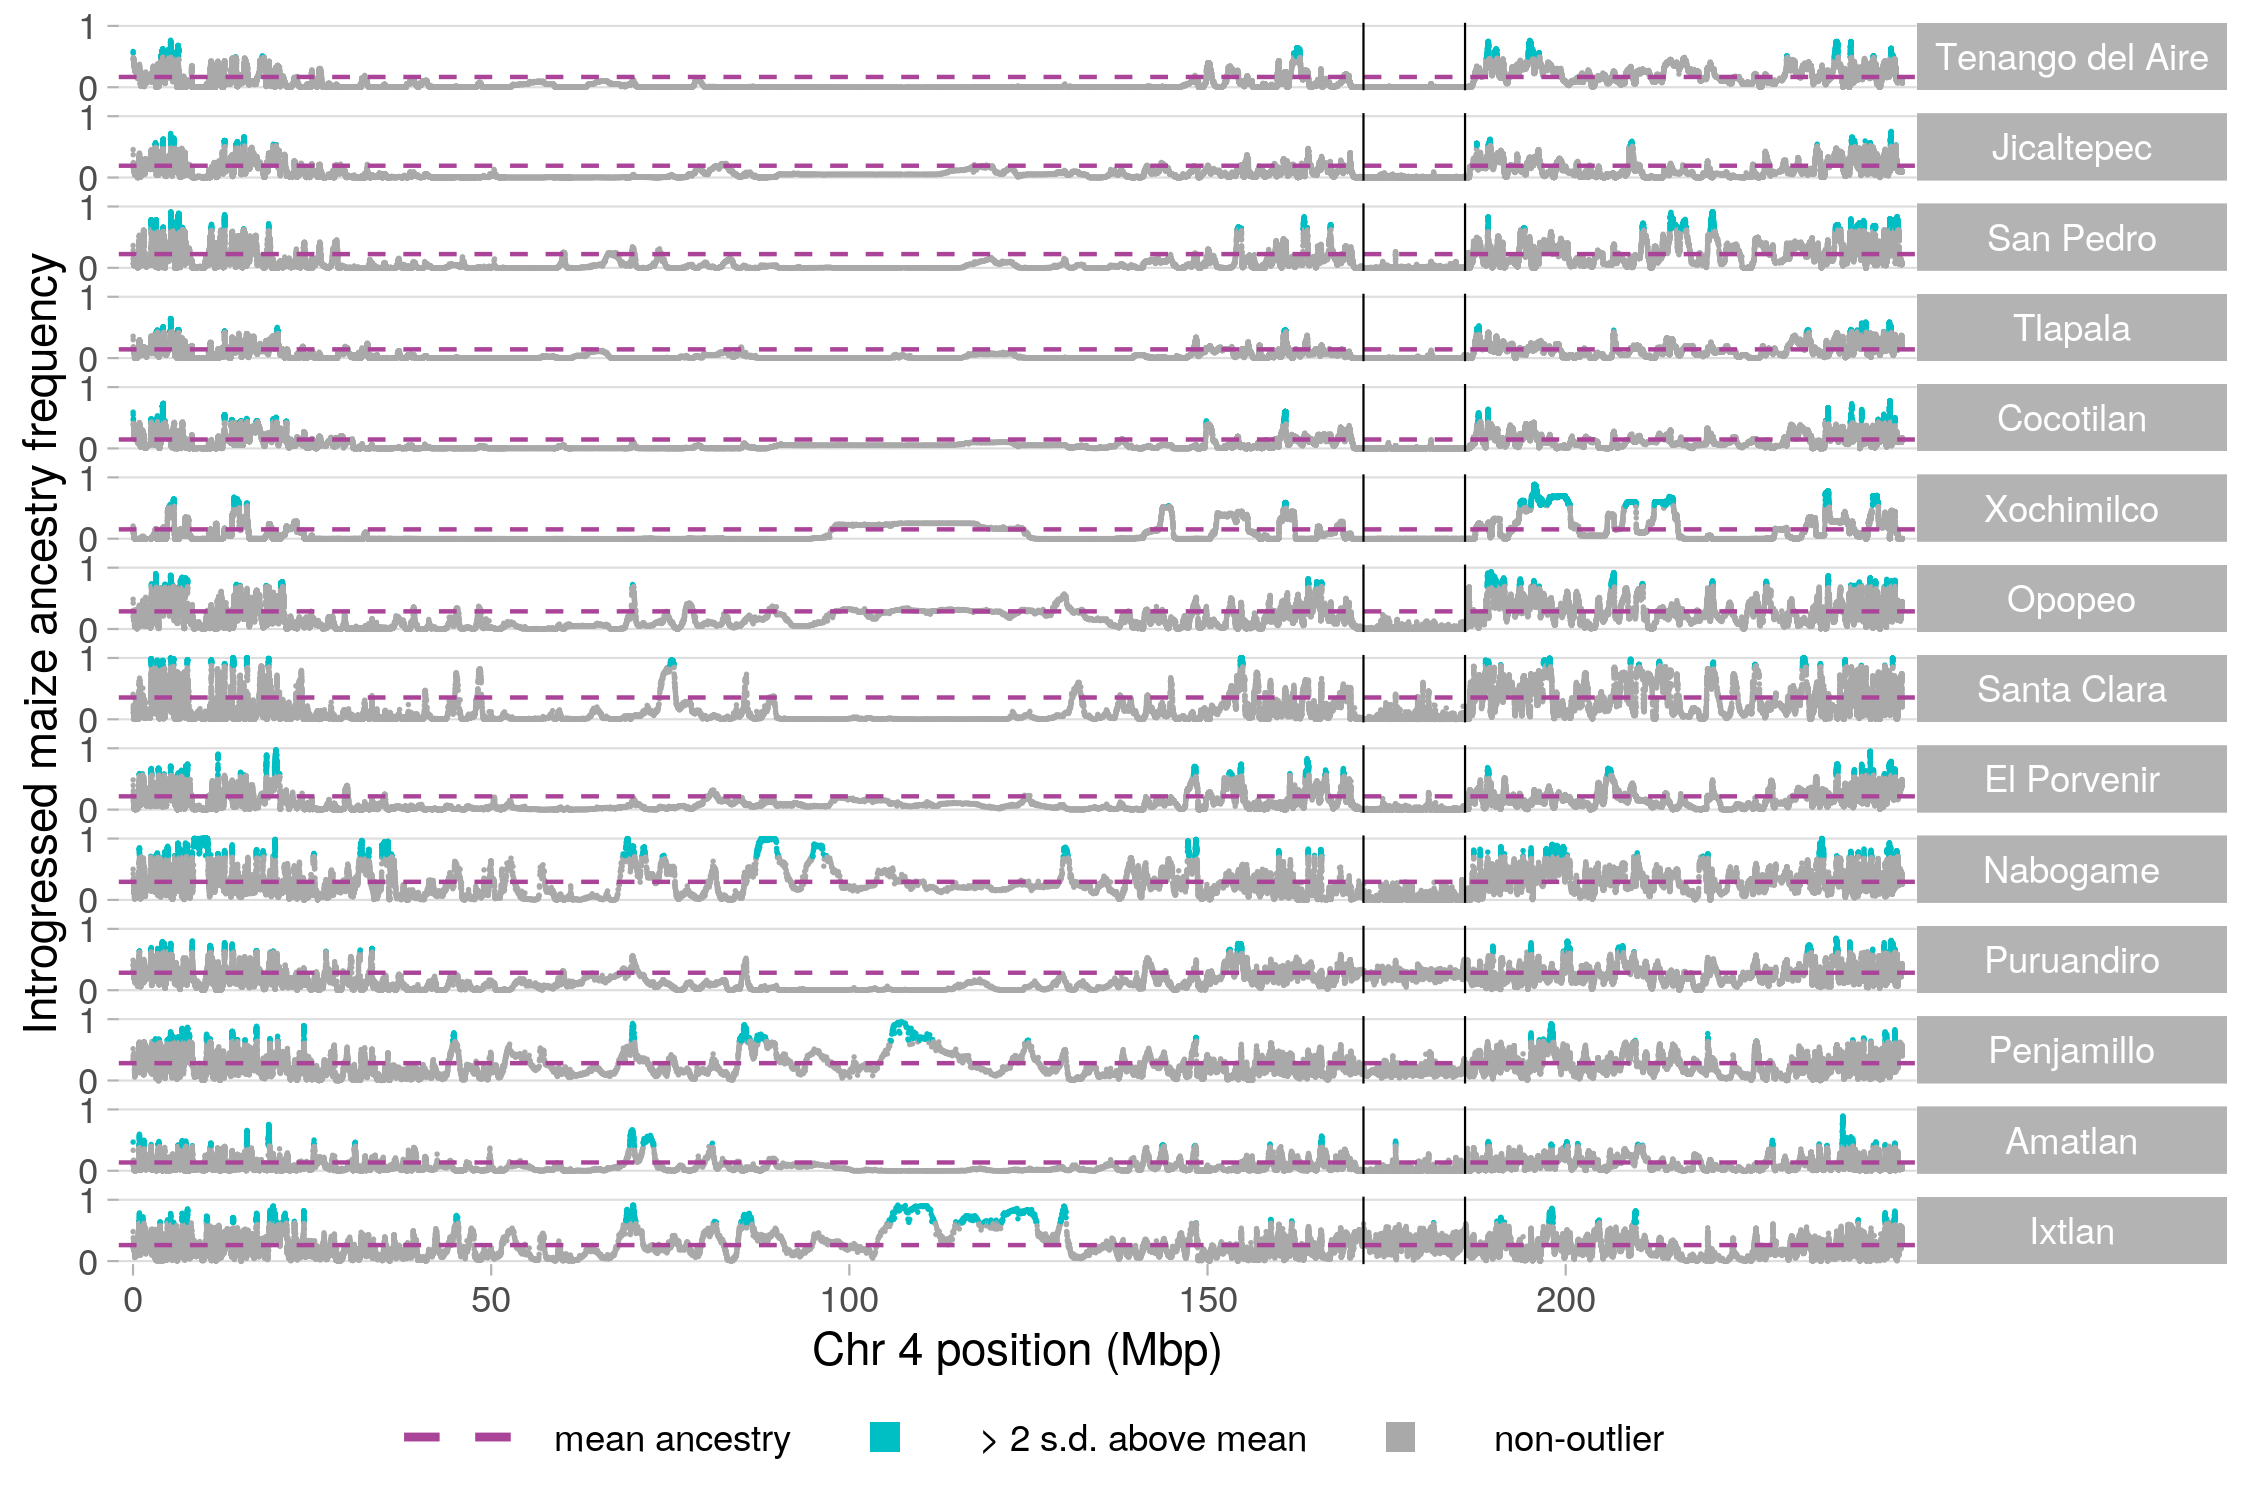
\includegraphics[width=.85\textwidth]{chapter2/figures/mexicana_shared_outliers_chr_4.png}
\caption{\color{Gray} \textbf{Introgression in \mexicana populations across chromosome 4} Vertical lines indicate the coordinates for \textit{Inv4m}.}
\label{mexicana_chr4}
\end{figure}

\begin{figure}[ht]
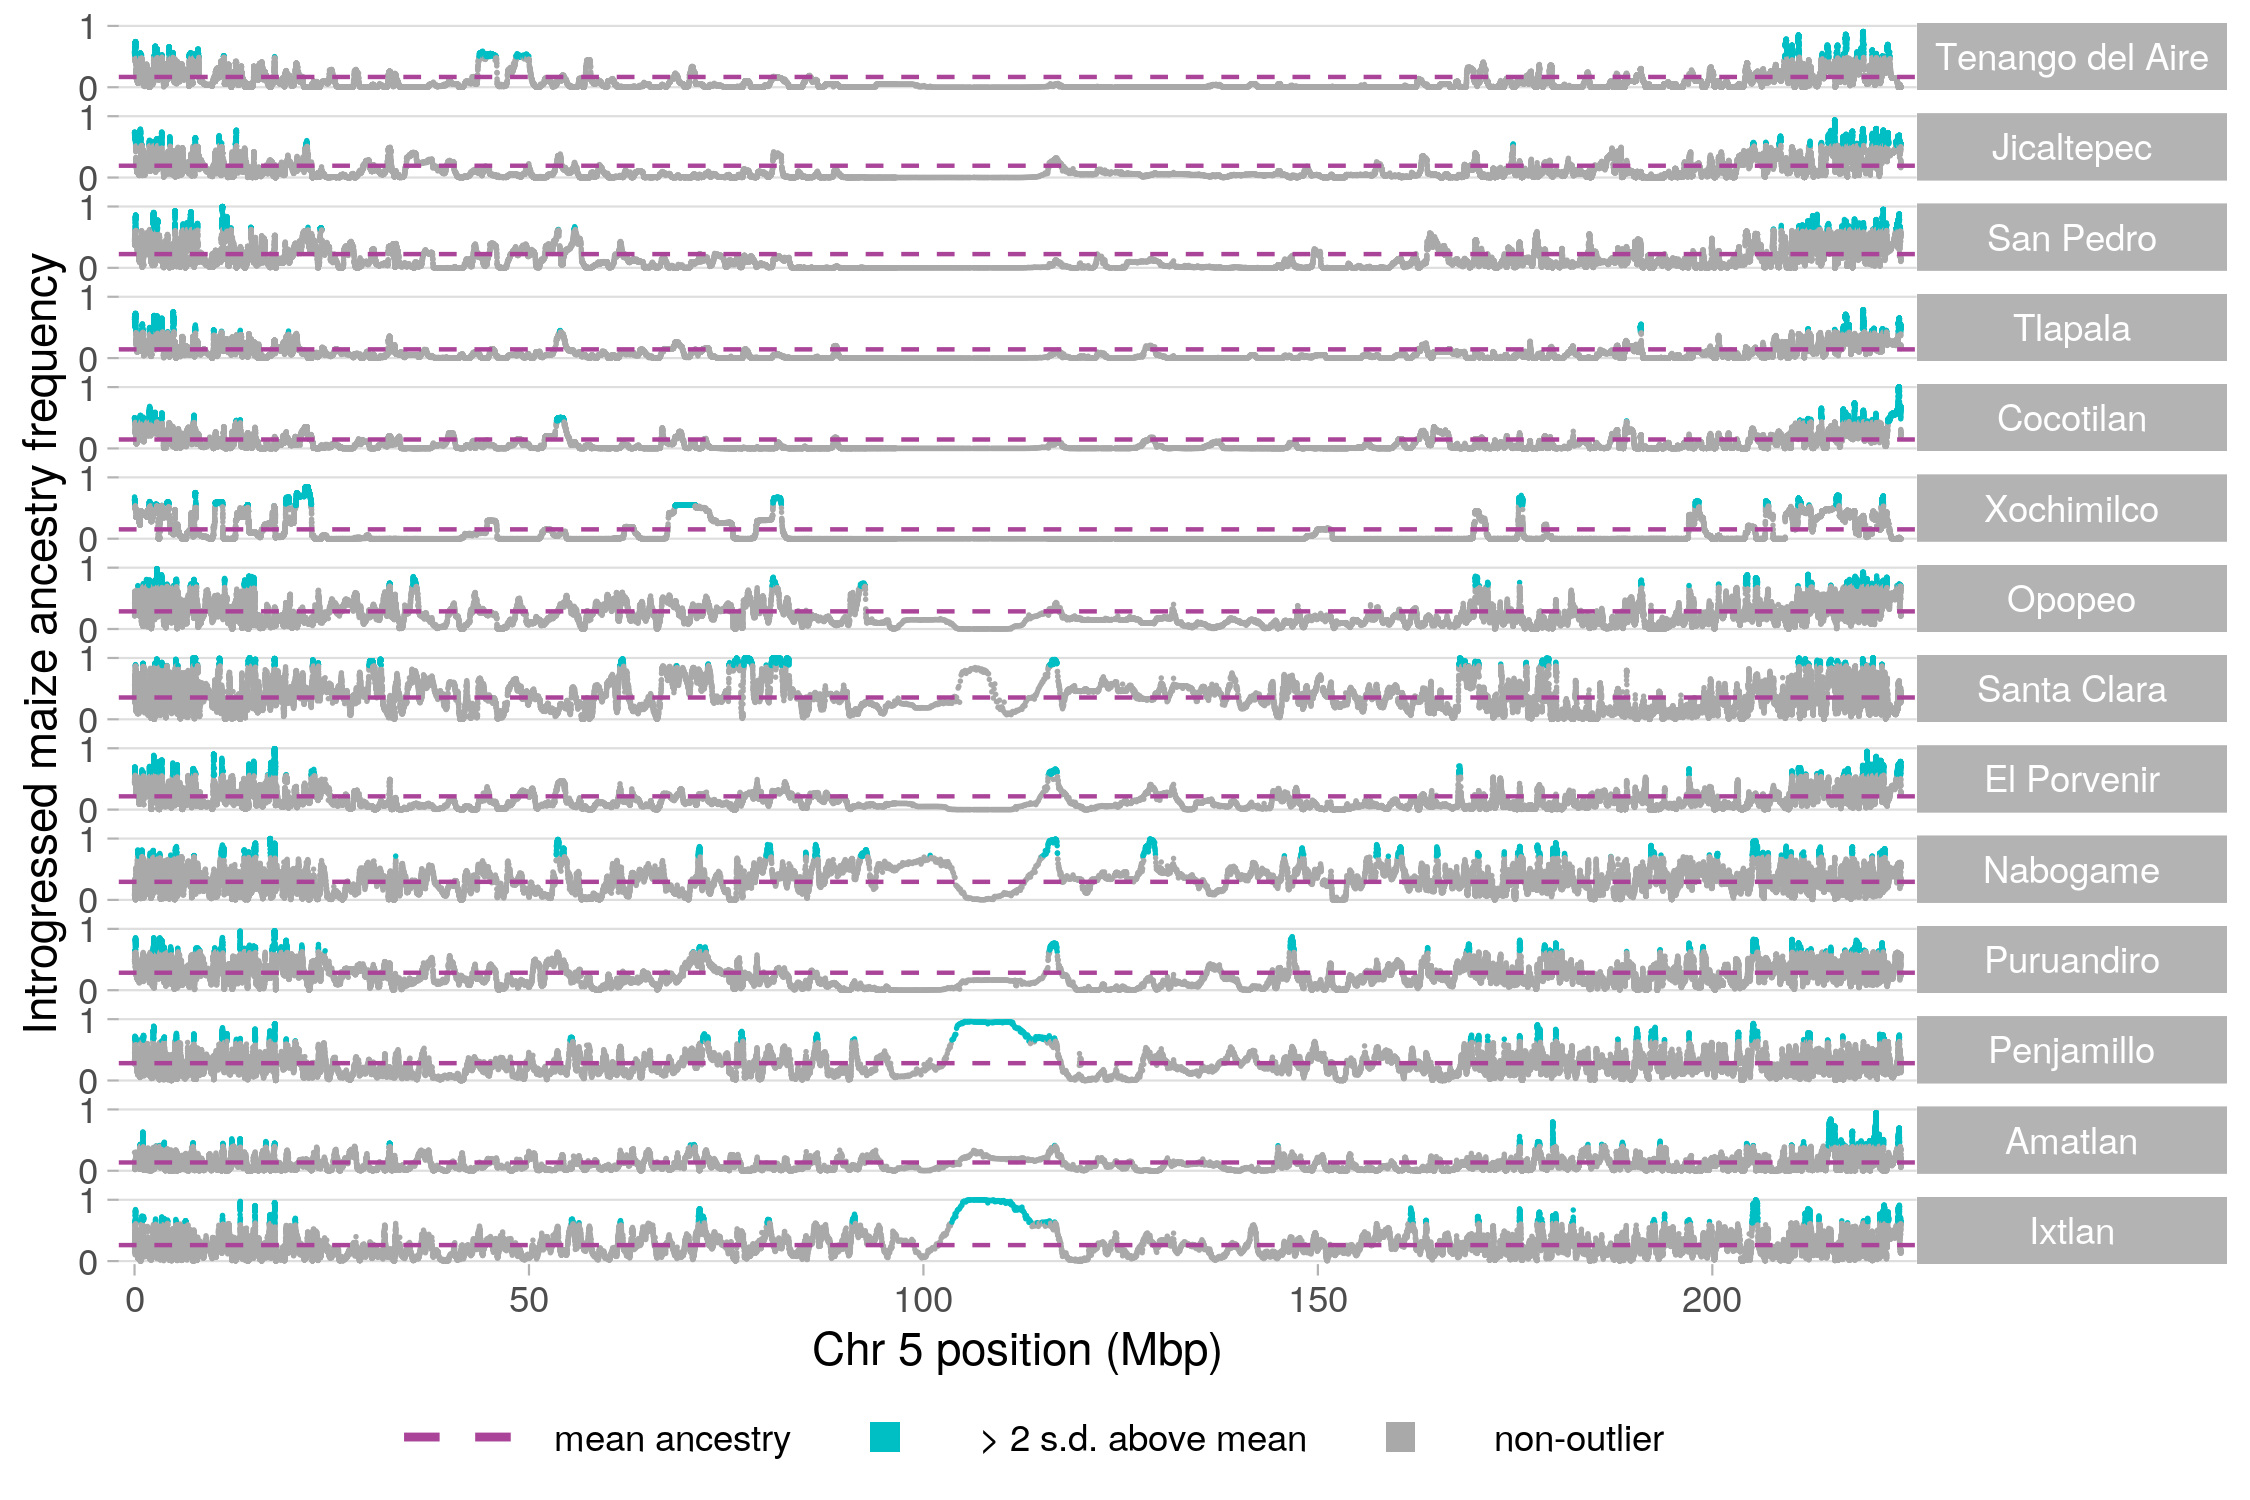
\includegraphics[width=.85\textwidth]{chapter2/figures/mexicana_shared_outliers_chr_5.png}
\caption{\color{Gray} \textbf{Introgression in \mexicana populations across chromosome 5}}
\label{mexicana_chr5}
\end{figure}

\begin{figure}[ht]
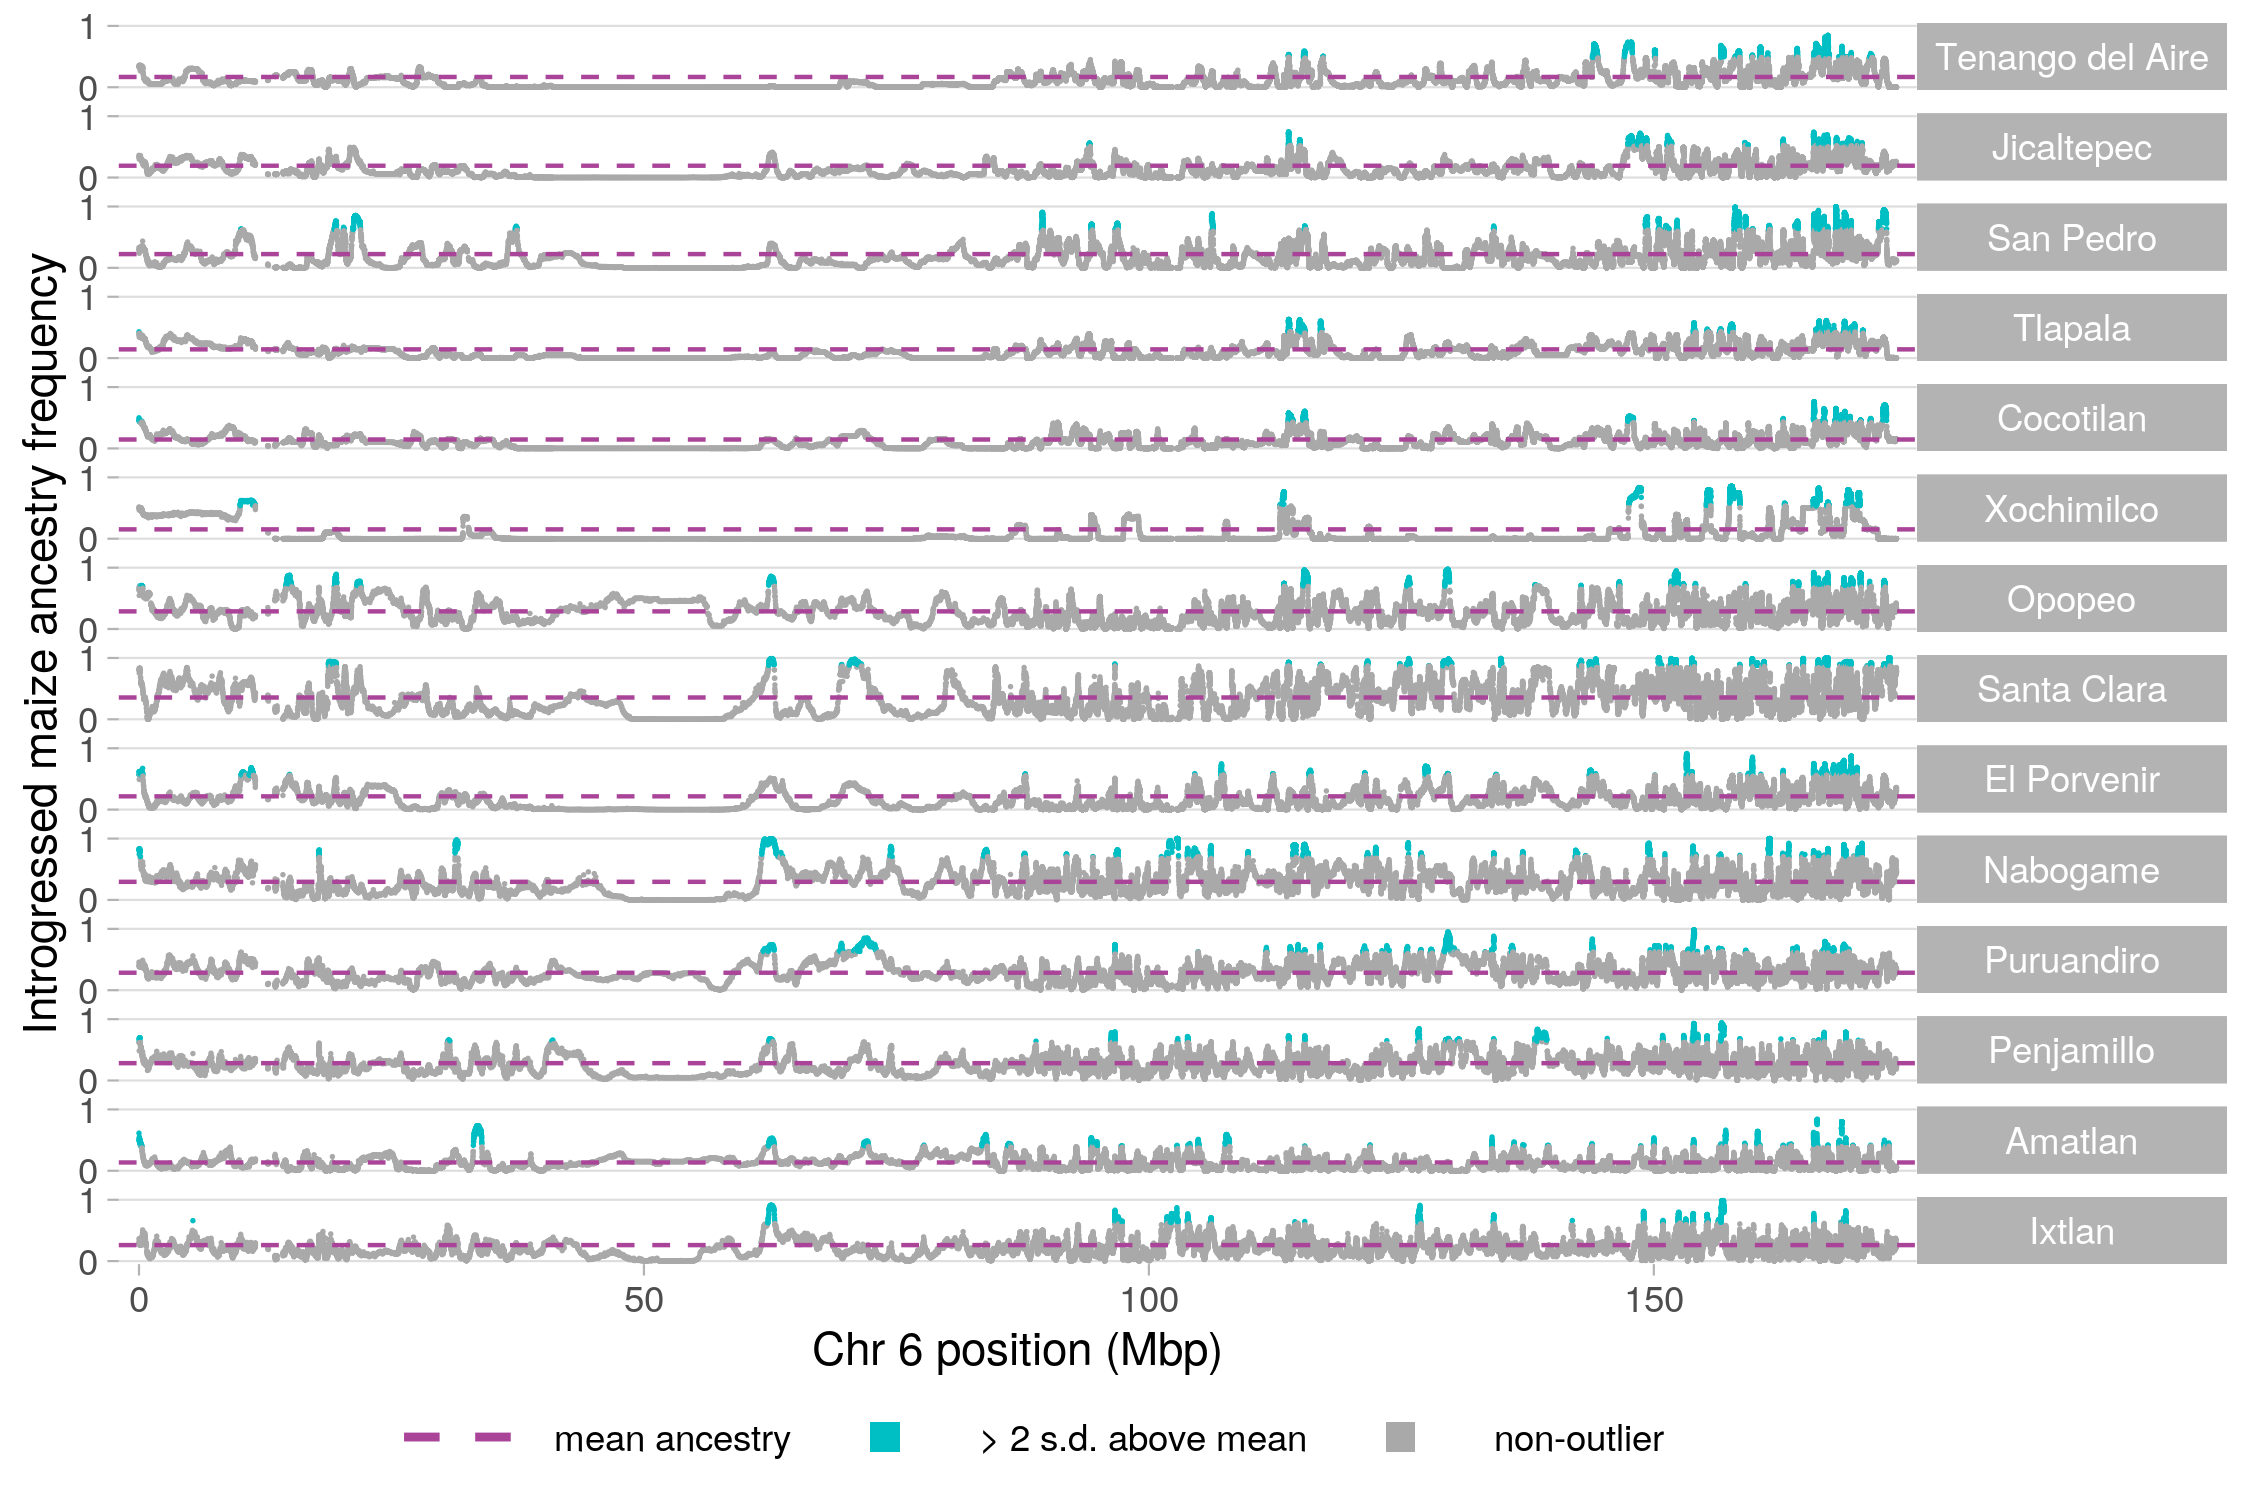
\includegraphics[width=.85\textwidth]{chapter2/figures/mexicana_shared_outliers_chr_6.png}
\caption{\color{Gray} \textbf{Introgression in \mexicana populations across chromosome 6}}
\label{mexicana_chr6}
\end{figure}

\begin{figure}[ht]
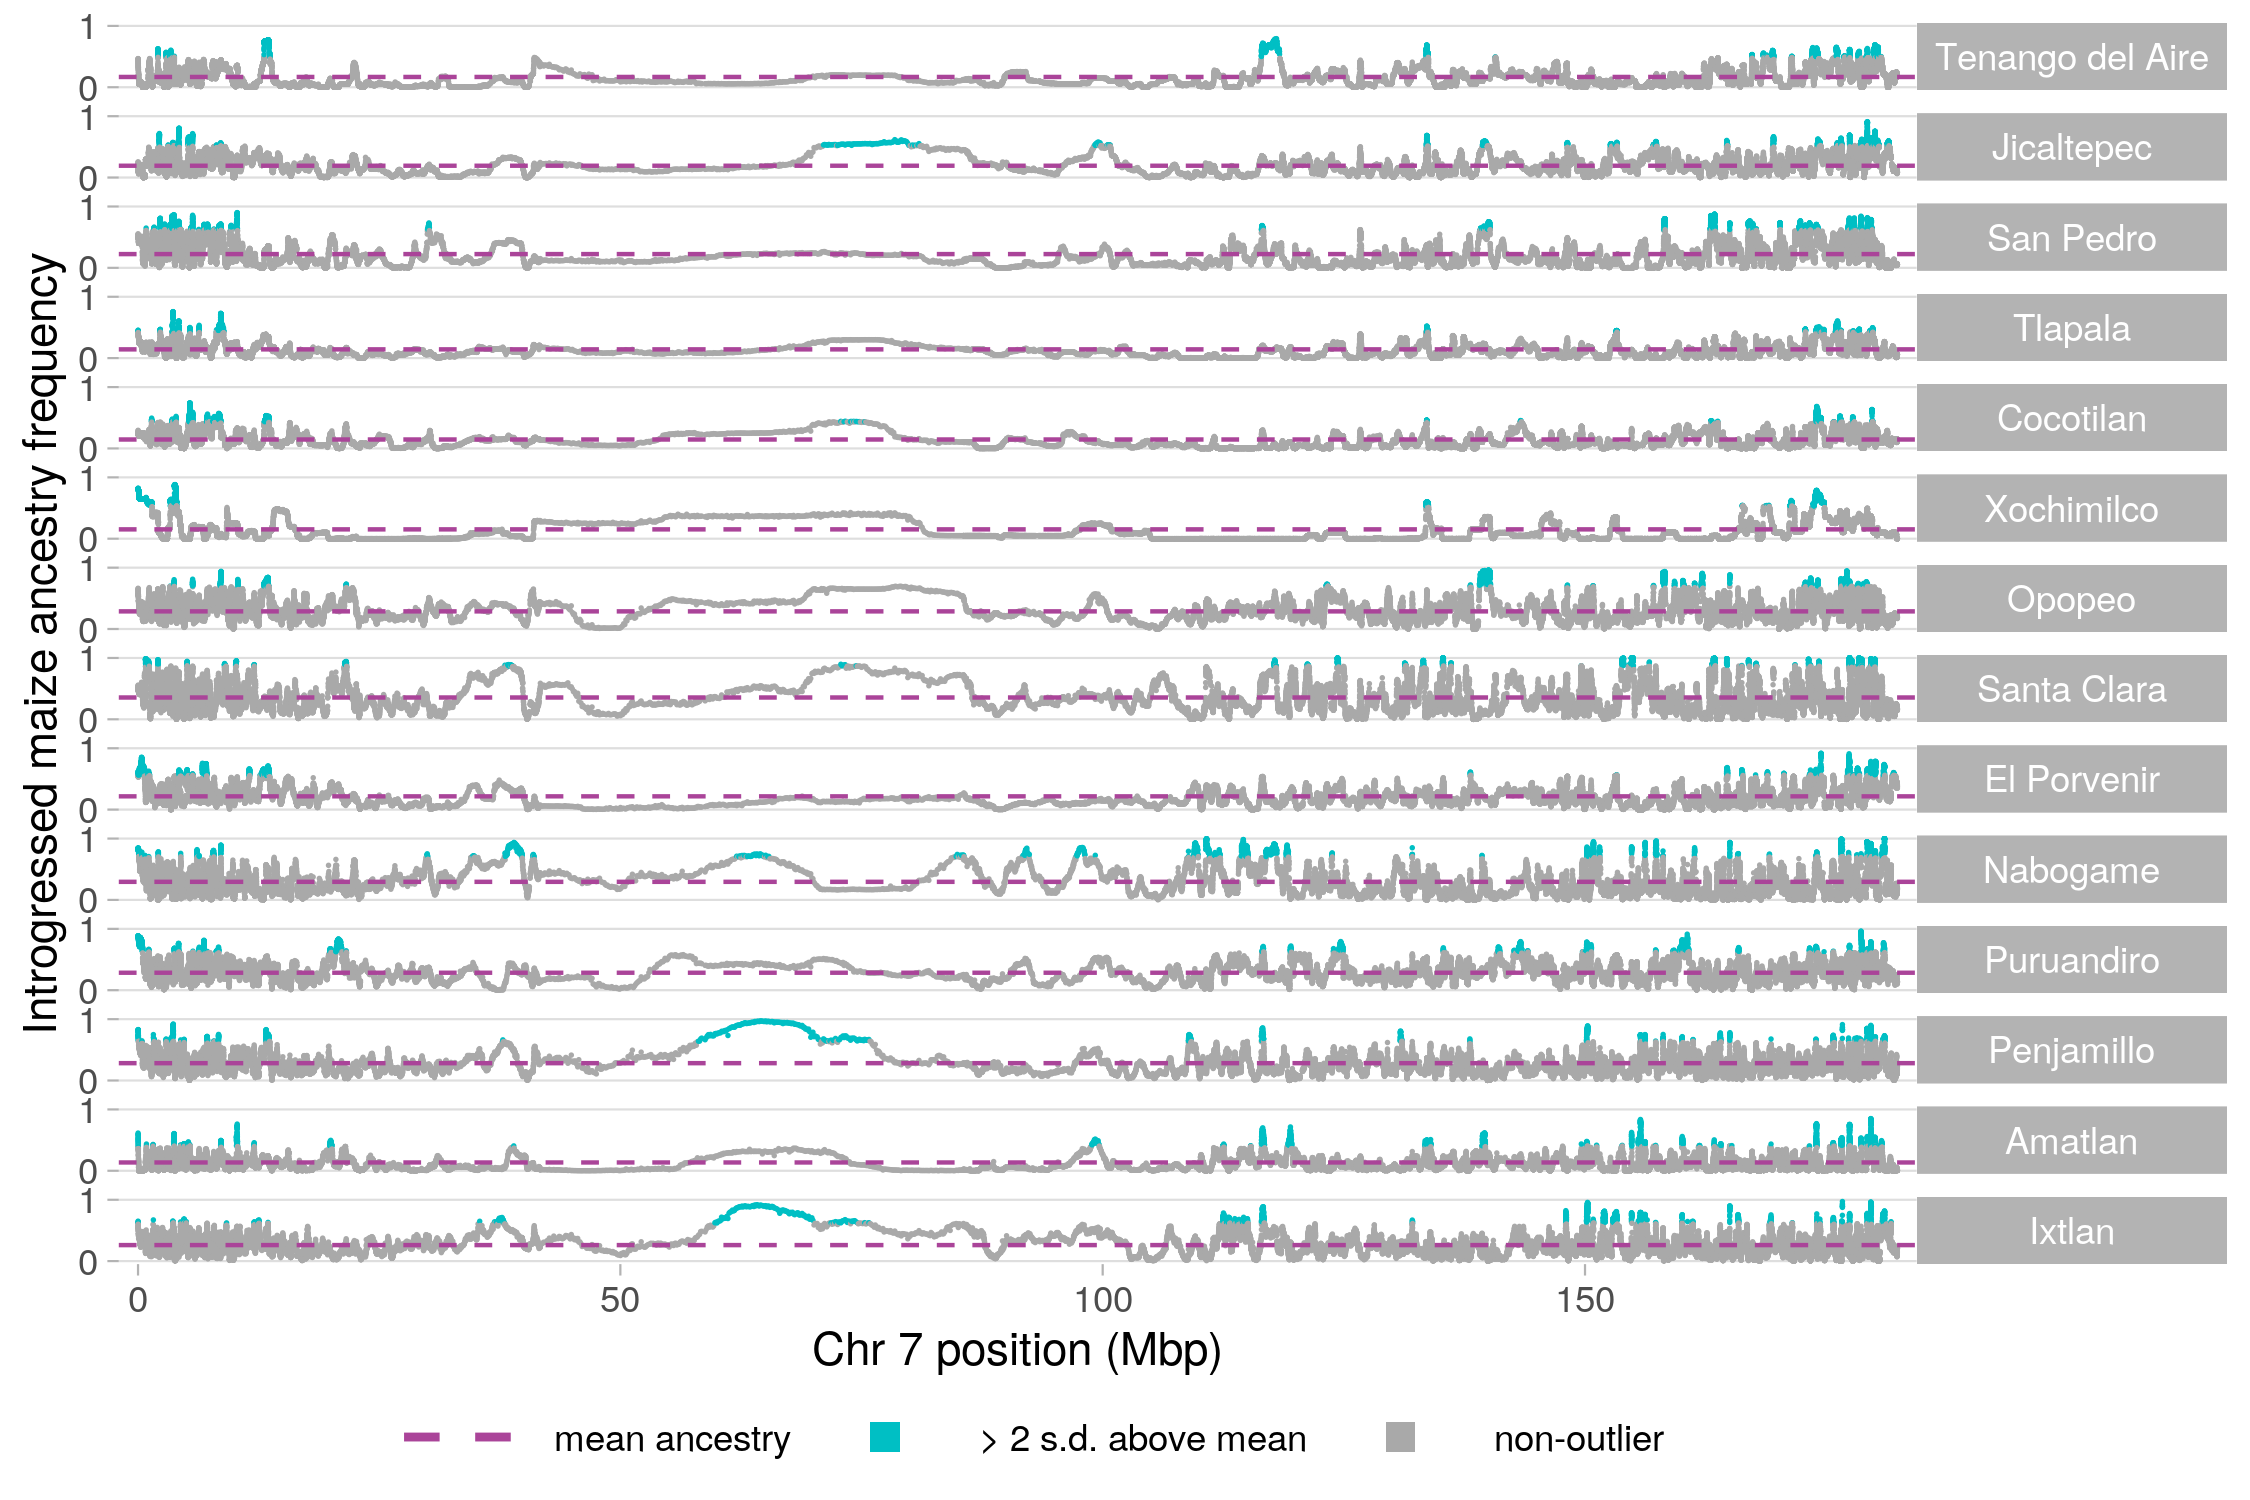
\includegraphics[width=.85\textwidth]{chapter2/figures/mexicana_shared_outliers_chr_7.png}
\caption{\color{Gray} \textbf{Introgression in \mexicana populations across chromosome 7}}
\label{mexicana_chr7}
\end{figure}

\begin{figure}[ht]
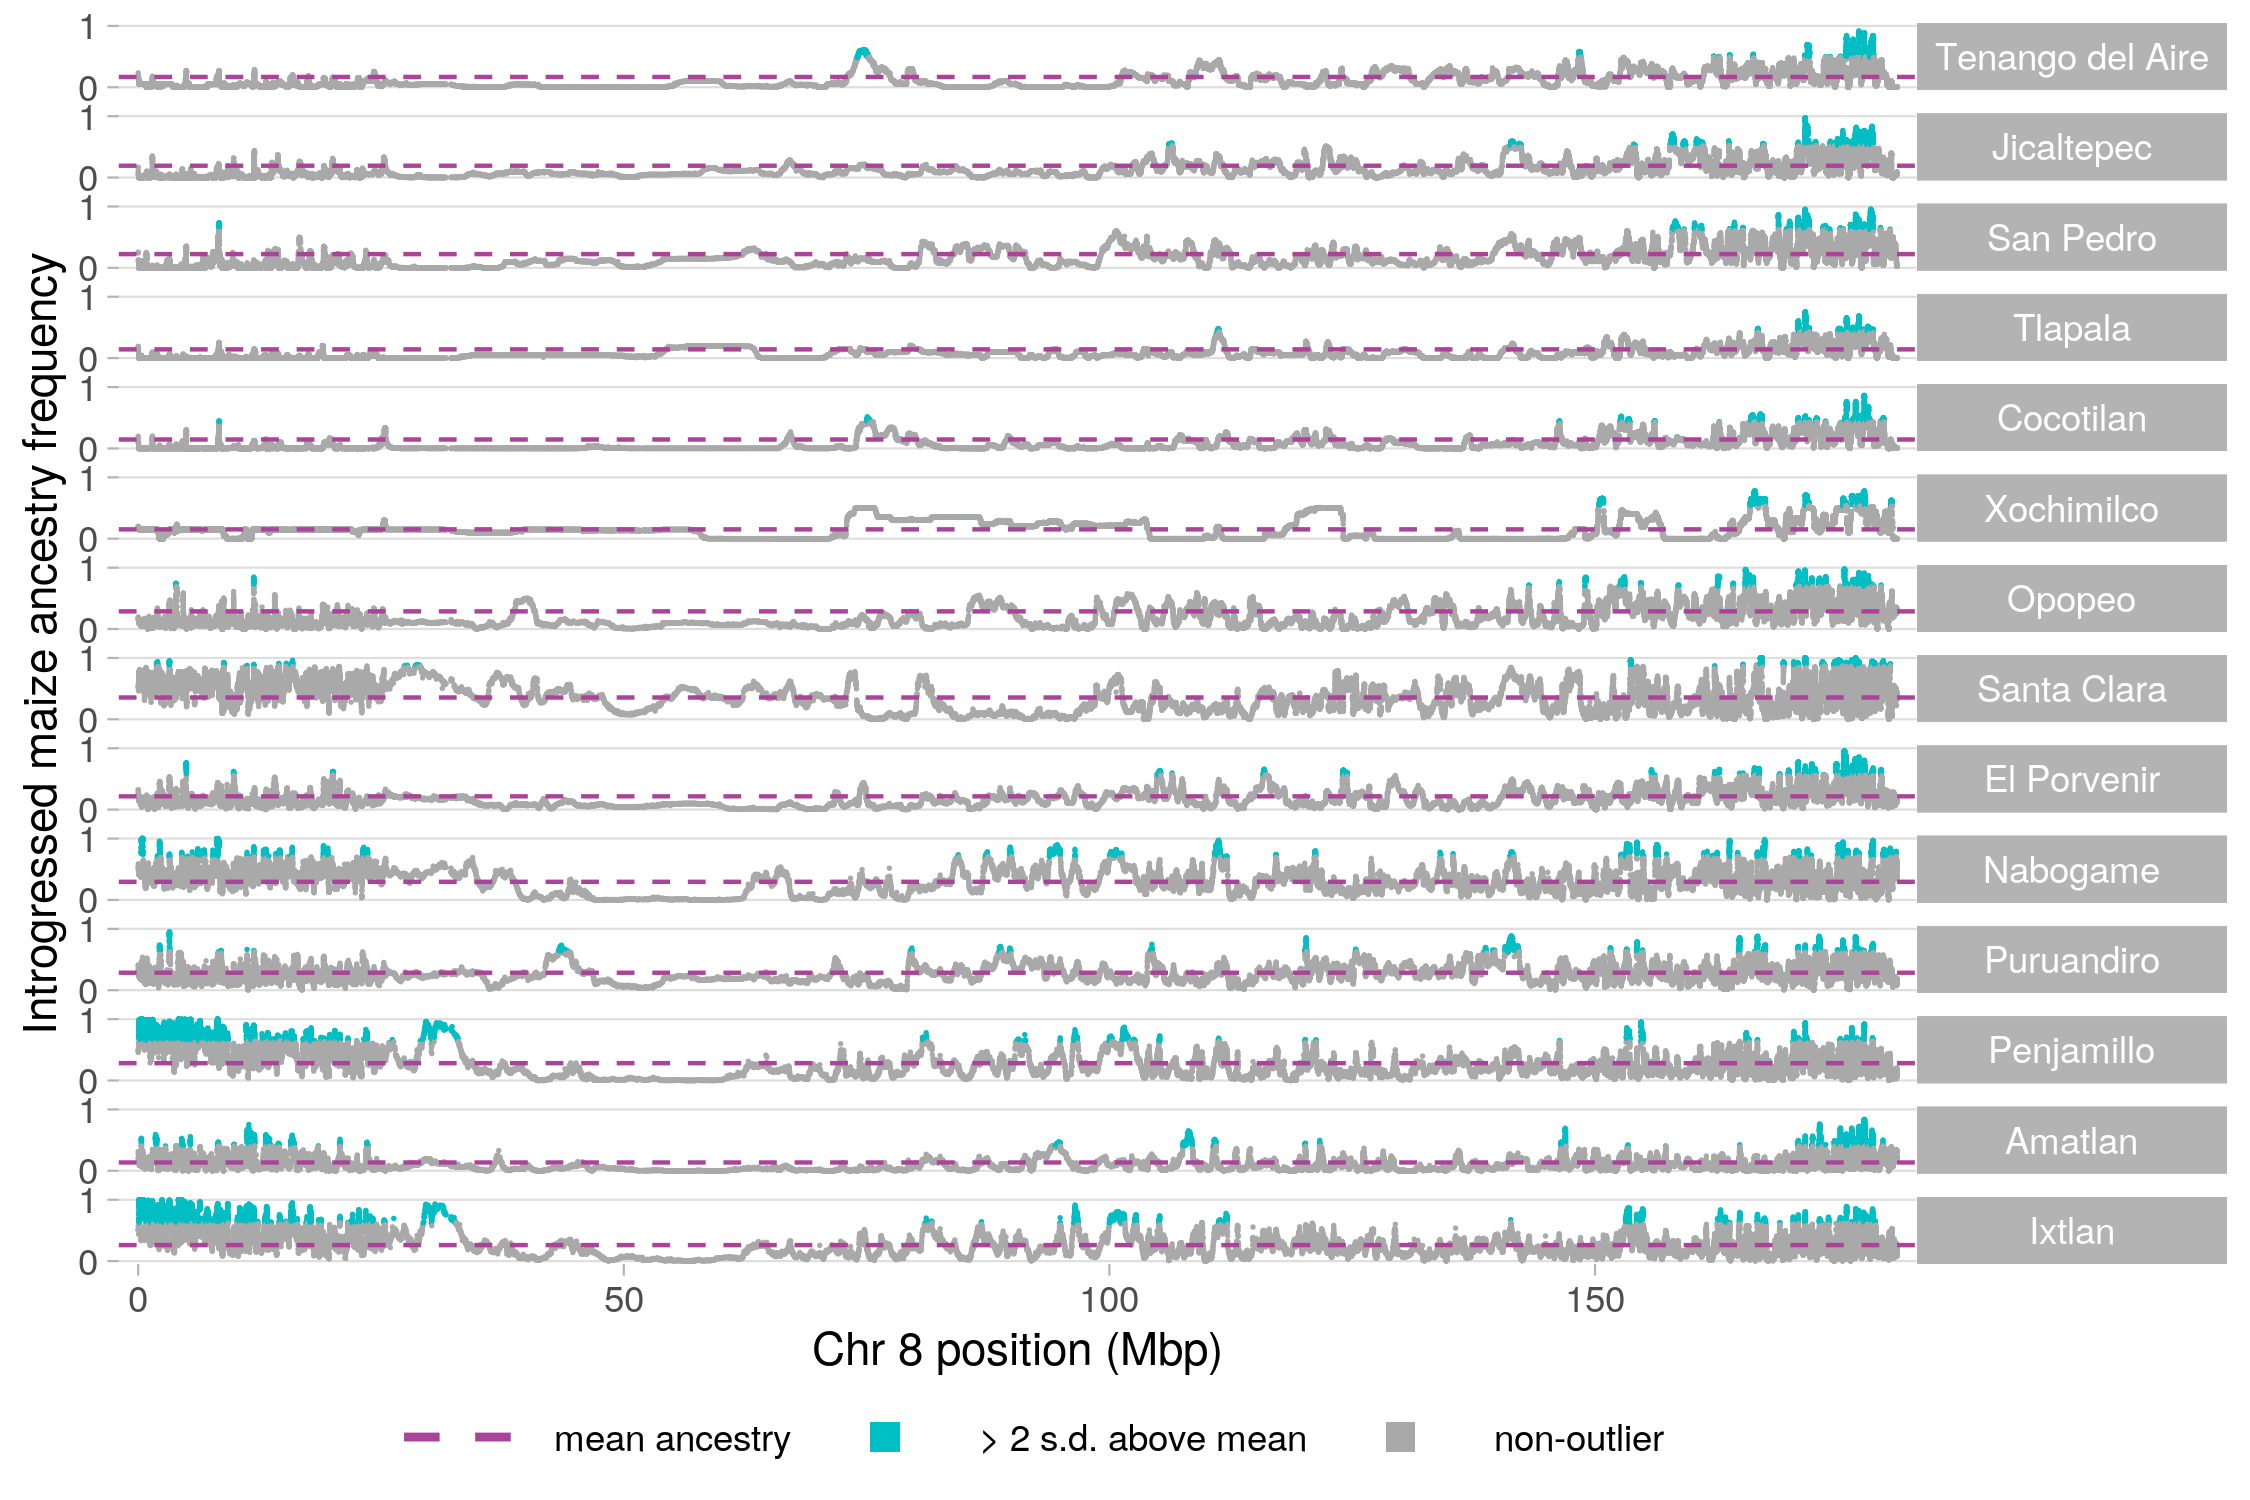
\includegraphics[width=.85\textwidth]{chapter2/figures/mexicana_shared_outliers_chr_8.png}
\caption{\color{Gray} \textbf{Introgression in \mexicana populations across chromosome 8}}
\label{mexicana_chr8}
\end{figure}

\begin{figure}[ht]
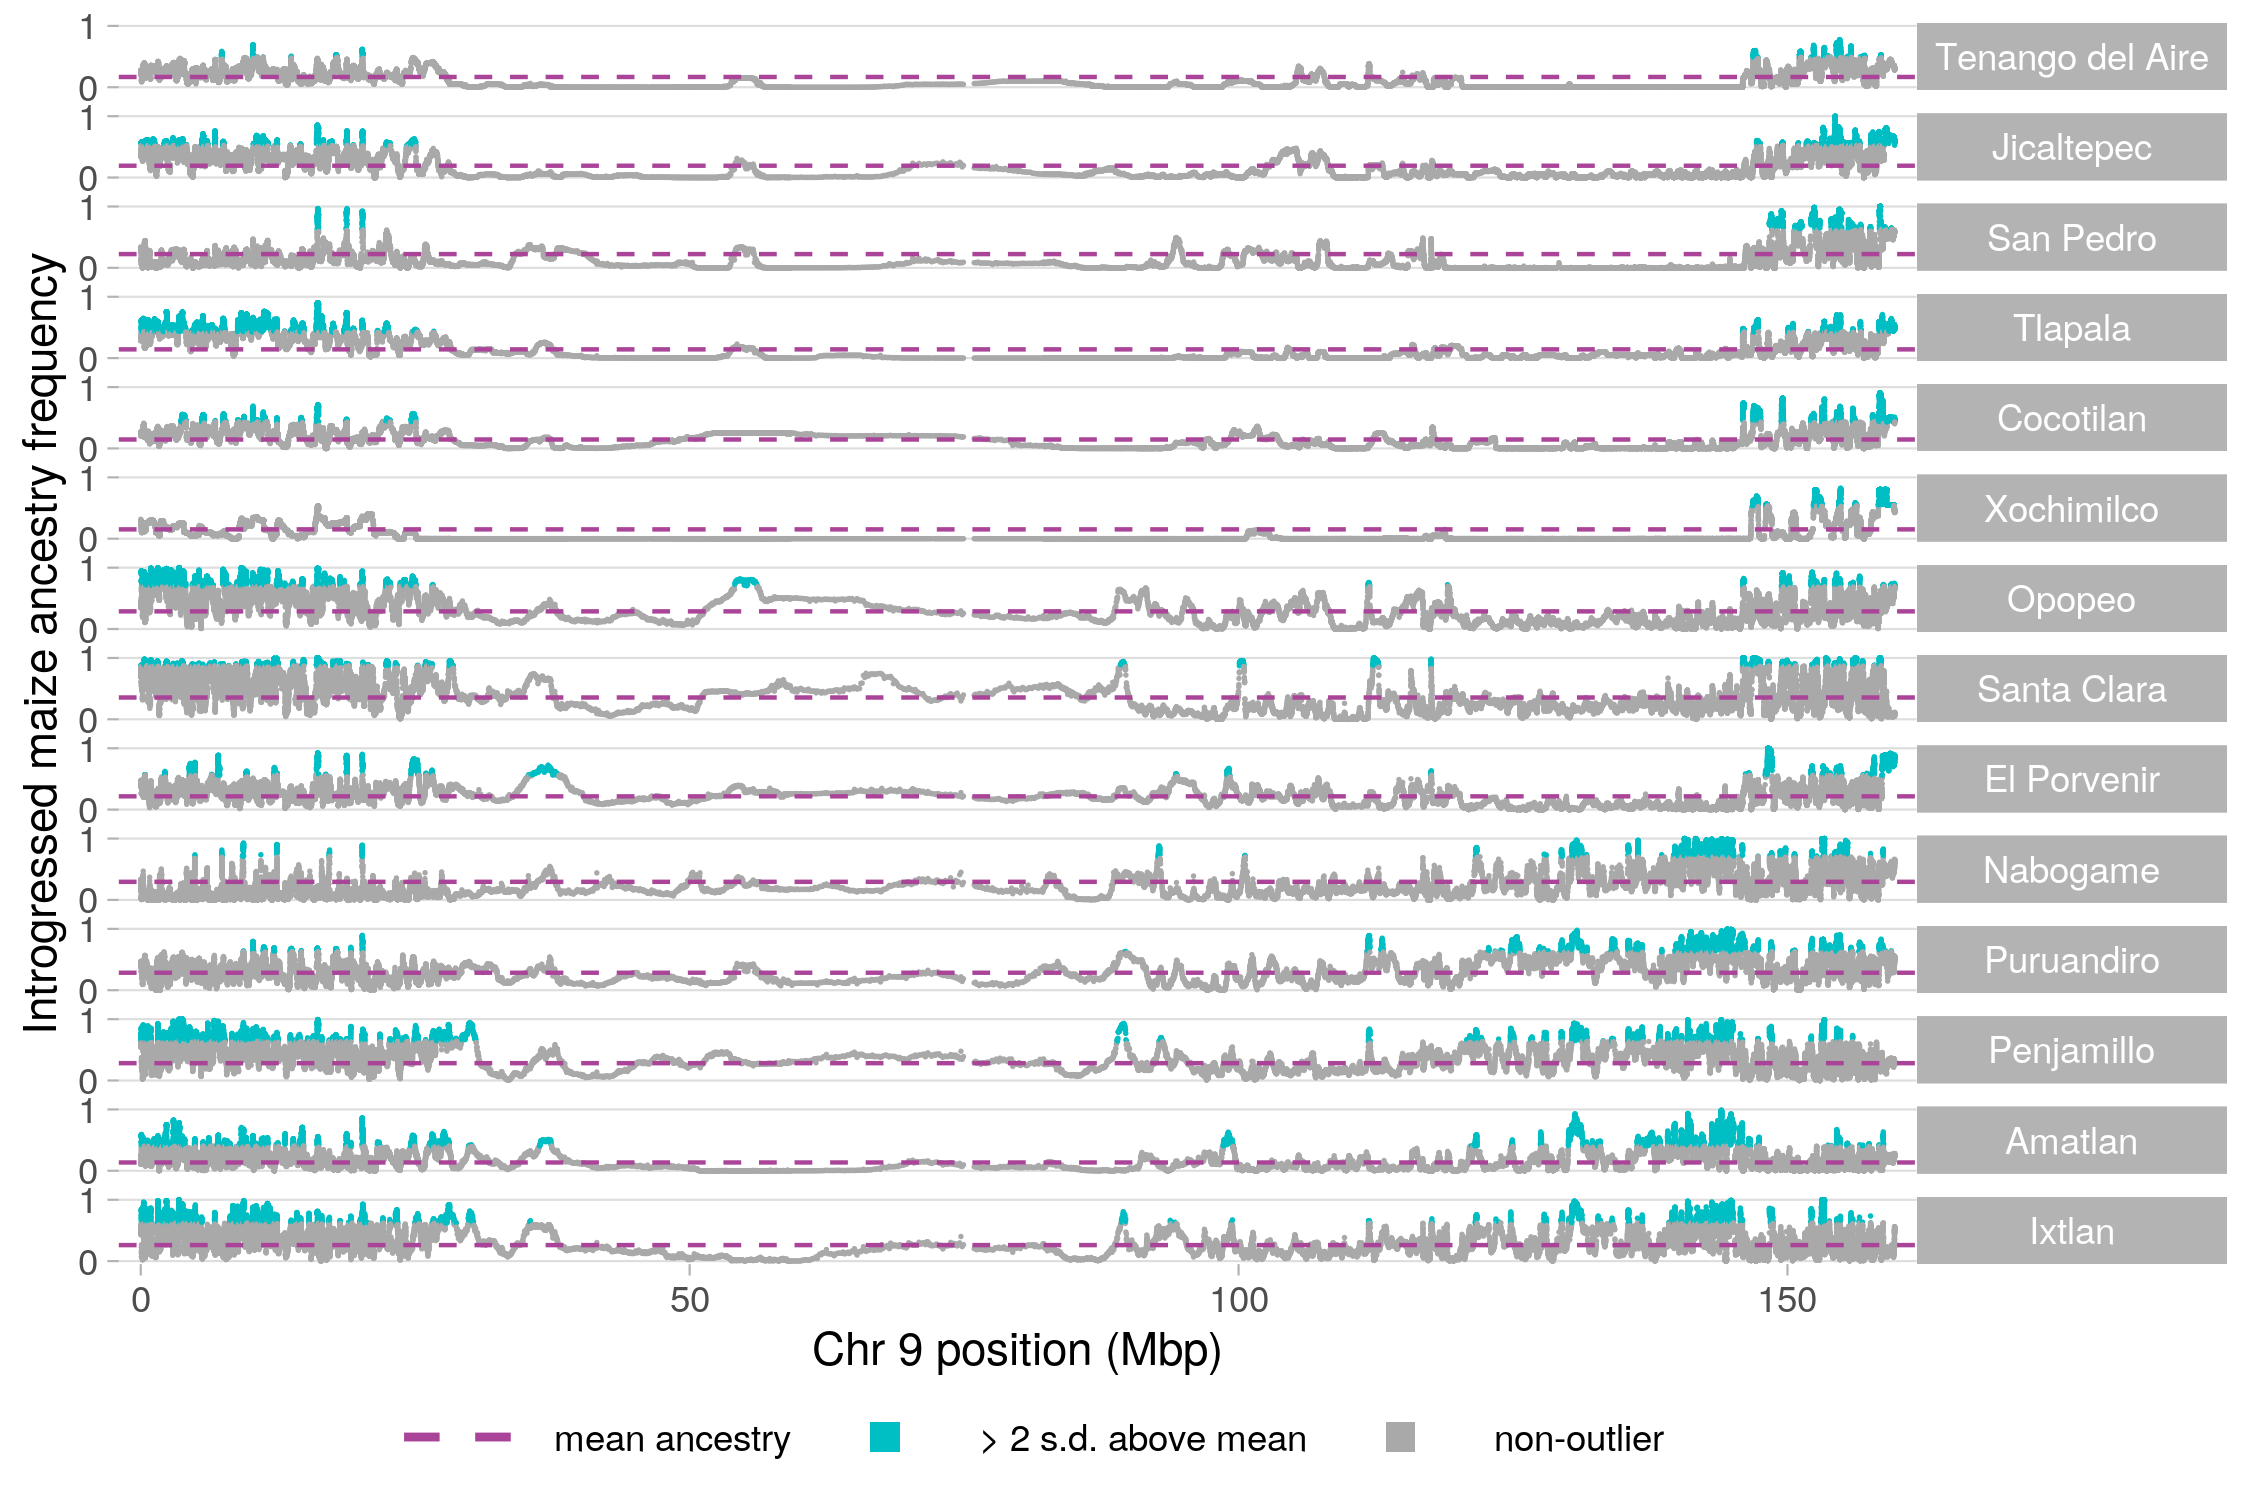
\includegraphics[width=.85\textwidth]{chapter2/figures/mexicana_shared_outliers_chr_9.png}
\caption{\color{Gray} \textbf{Introgression in \mexicana populations across chromosome 9}}
\label{mexicana_chr9}
\end{figure}

\begin{figure}[ht]
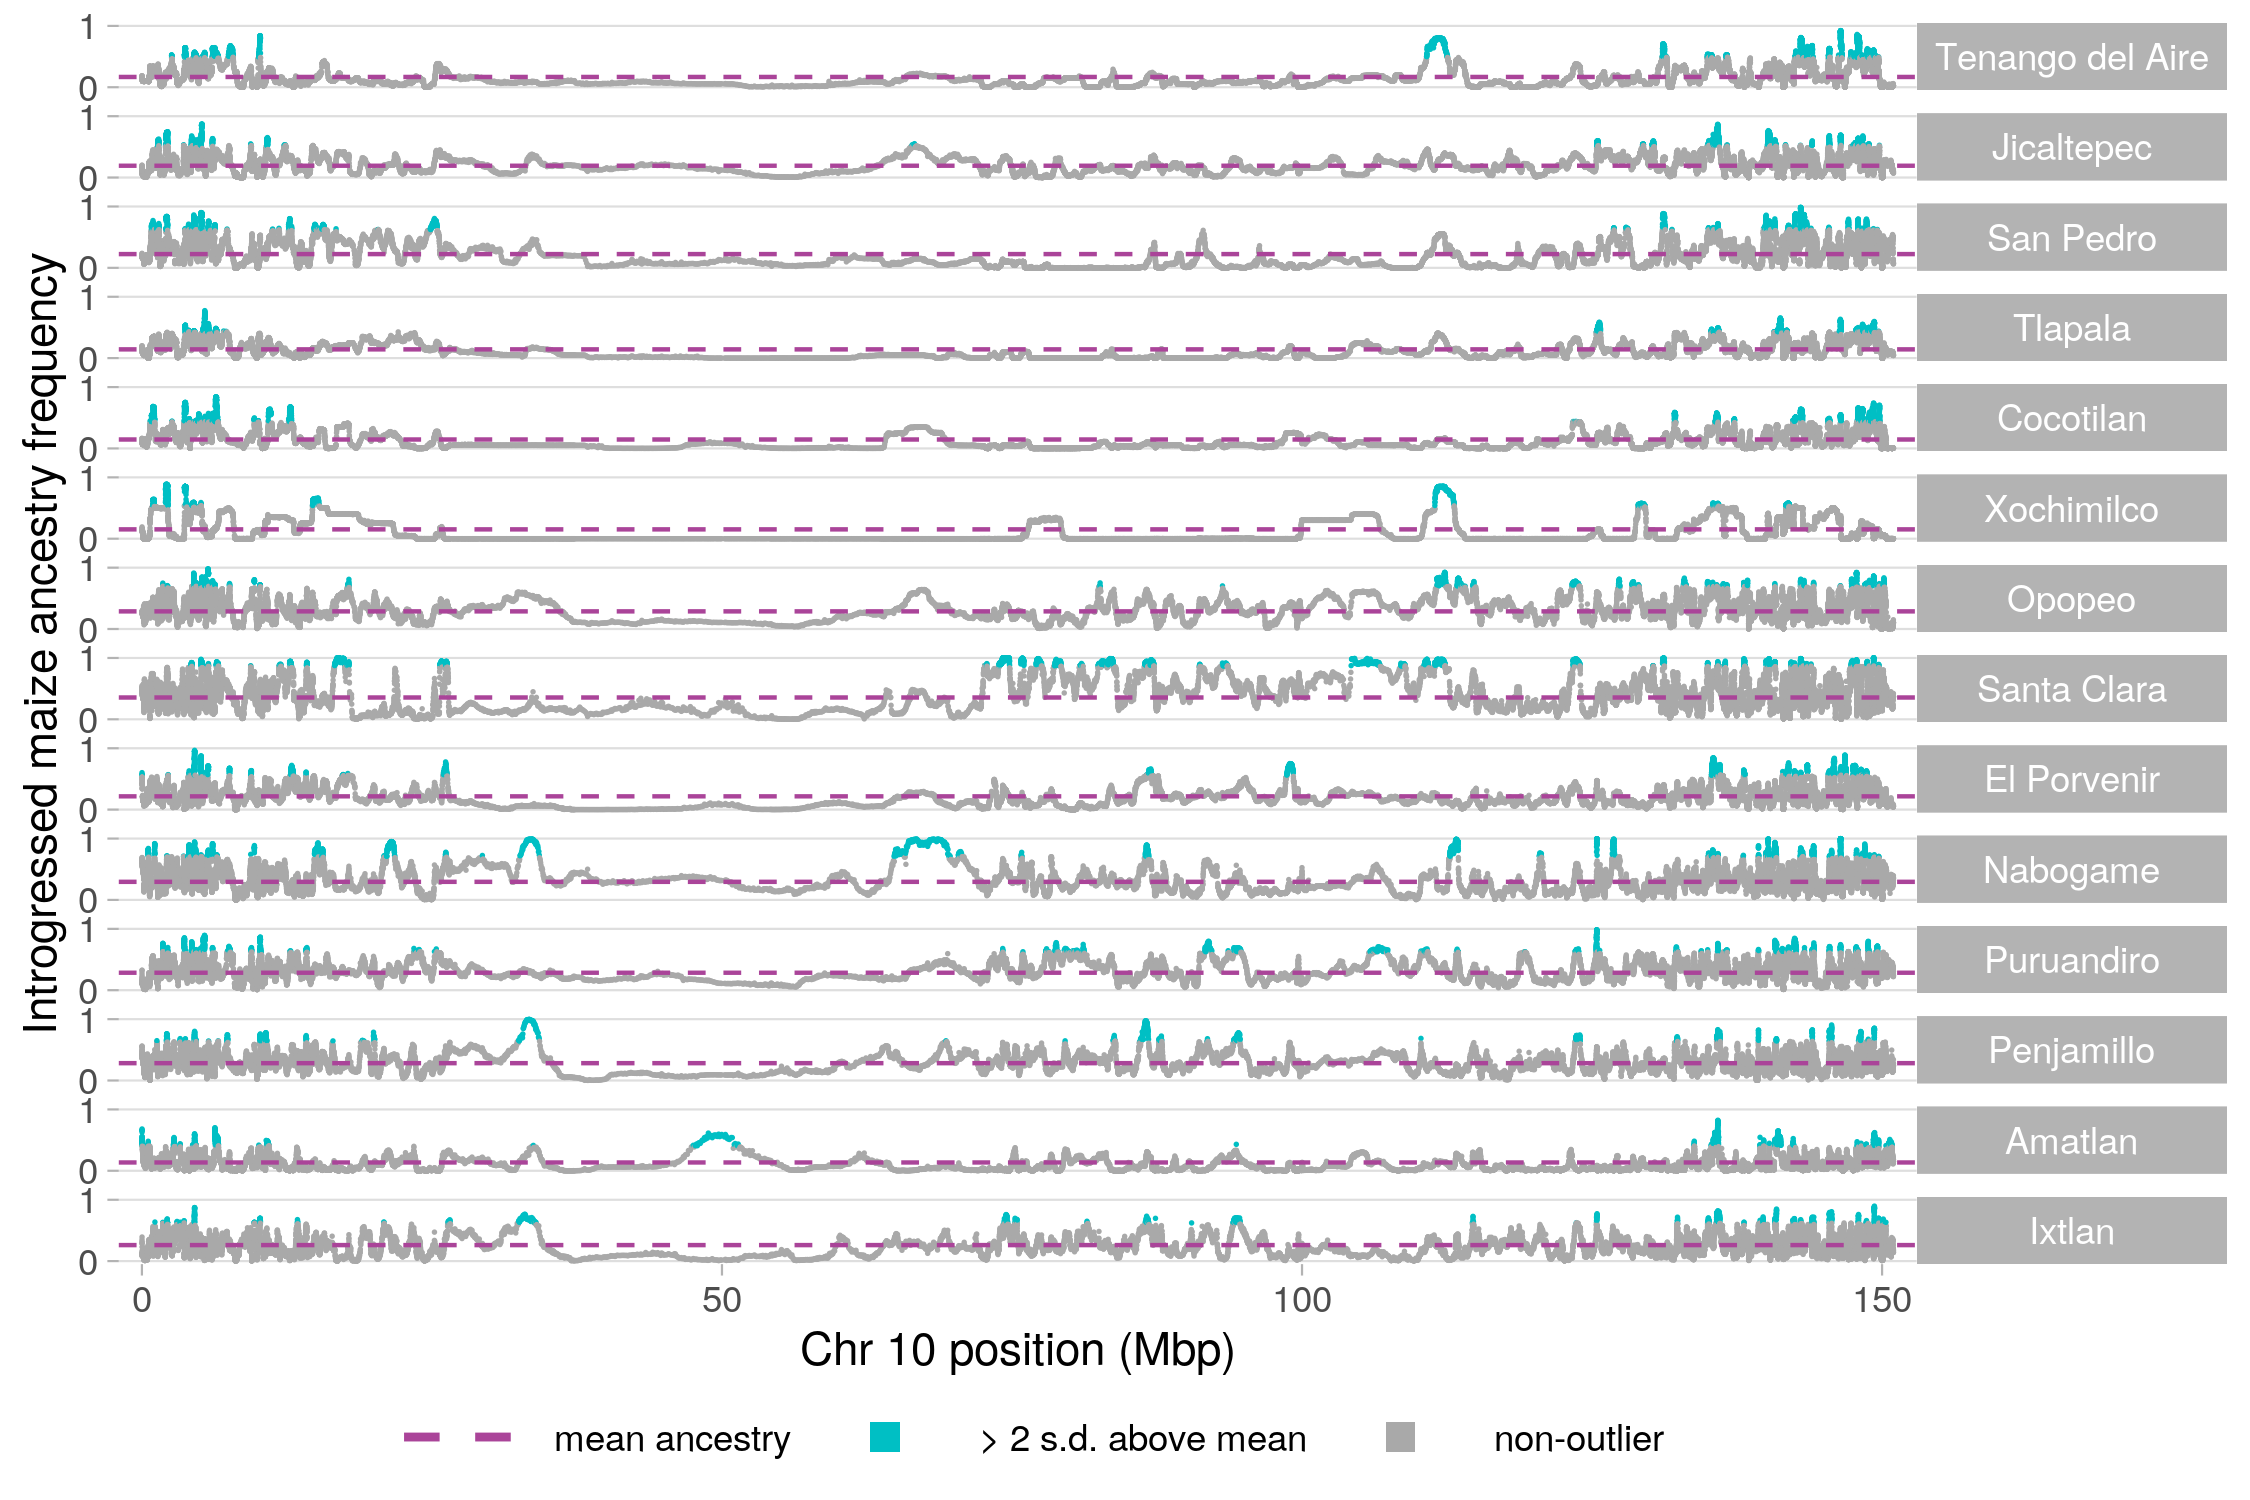
\includegraphics[width=.85\textwidth]{chapter2/figures/mexicana_shared_outliers_chr_10.png}
\caption{\color{Gray} \textbf{Introgression in \mexicana populations across chromosome 10}}
\label{mexicana_chr10}
\end{figure}

\begin{figure}[ht]
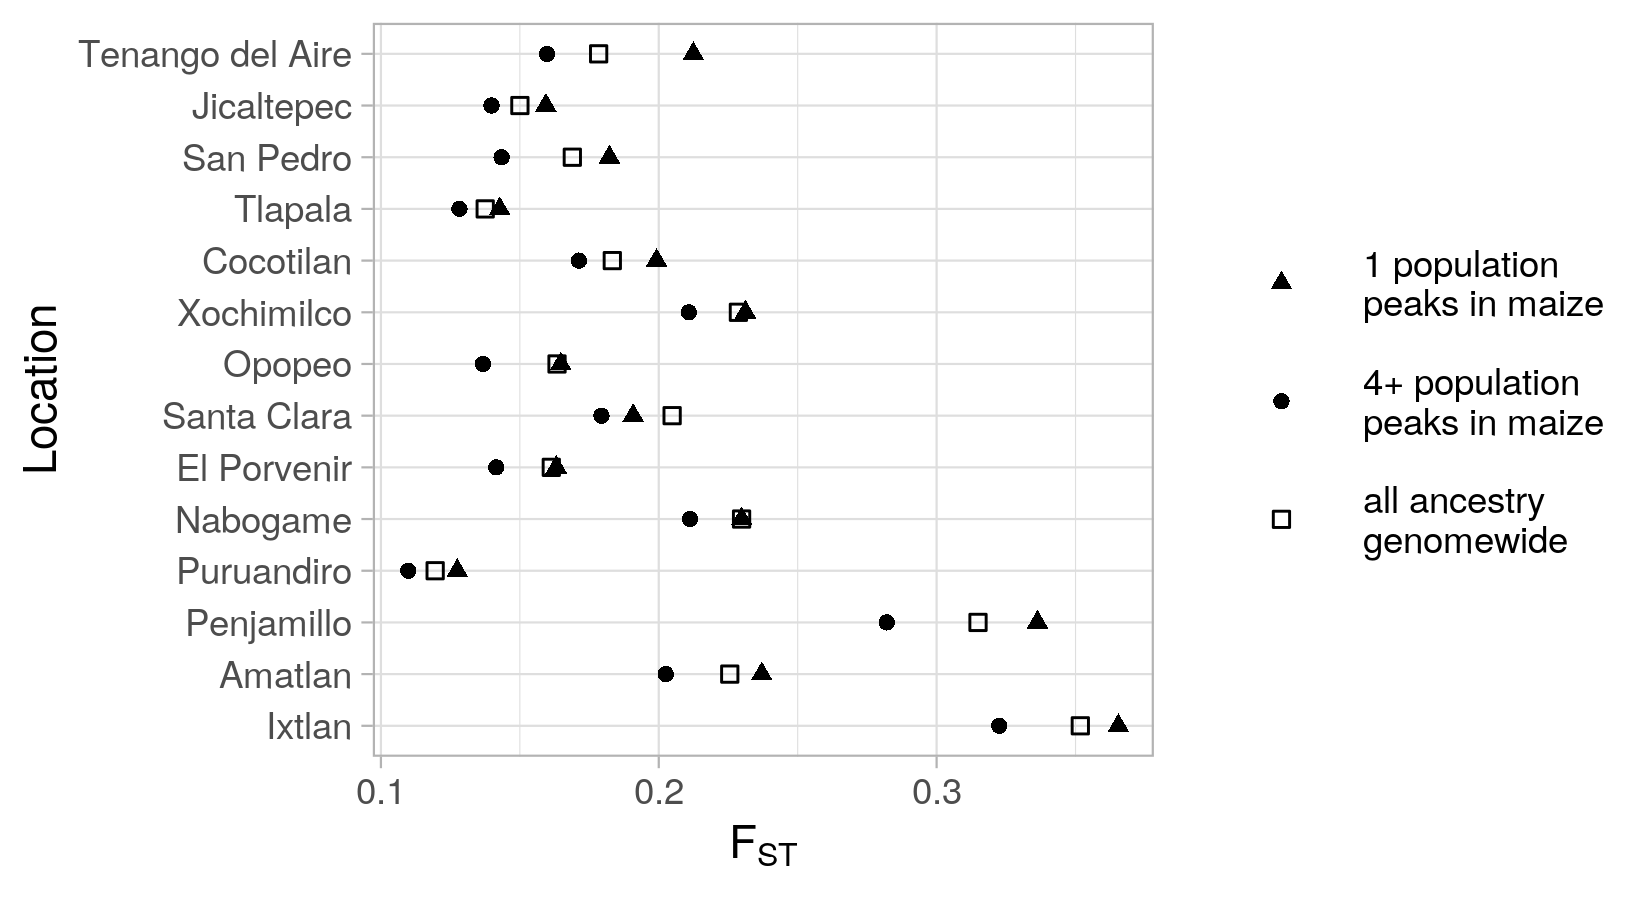
\includegraphics[width=\textwidth]{chapter2/figures/local_fst_within_mexicana_ancestry_peaks.png}
\caption{\color{Gray} \textbf{Differentiation ($F_{ST}$) between introgressed ancestry tracts and local \mexicana} Each point summarises $F_{ST}$ between \mexicana ancestry tracts within a focal maize population and \mexicana ancestry tracts within the local \mexicana population sampled at the same site. Within-\mexicana ancestry $F_{ST}$ is presented separately for three subsets of the genome: introgression peaks found in the focal maize population only, peaks shared between the focal maize and at least 3 other maize populations, and a genomewide estimate.}
\label{local_fst_peaks}
\end{figure}

\begin{figure}[ht]
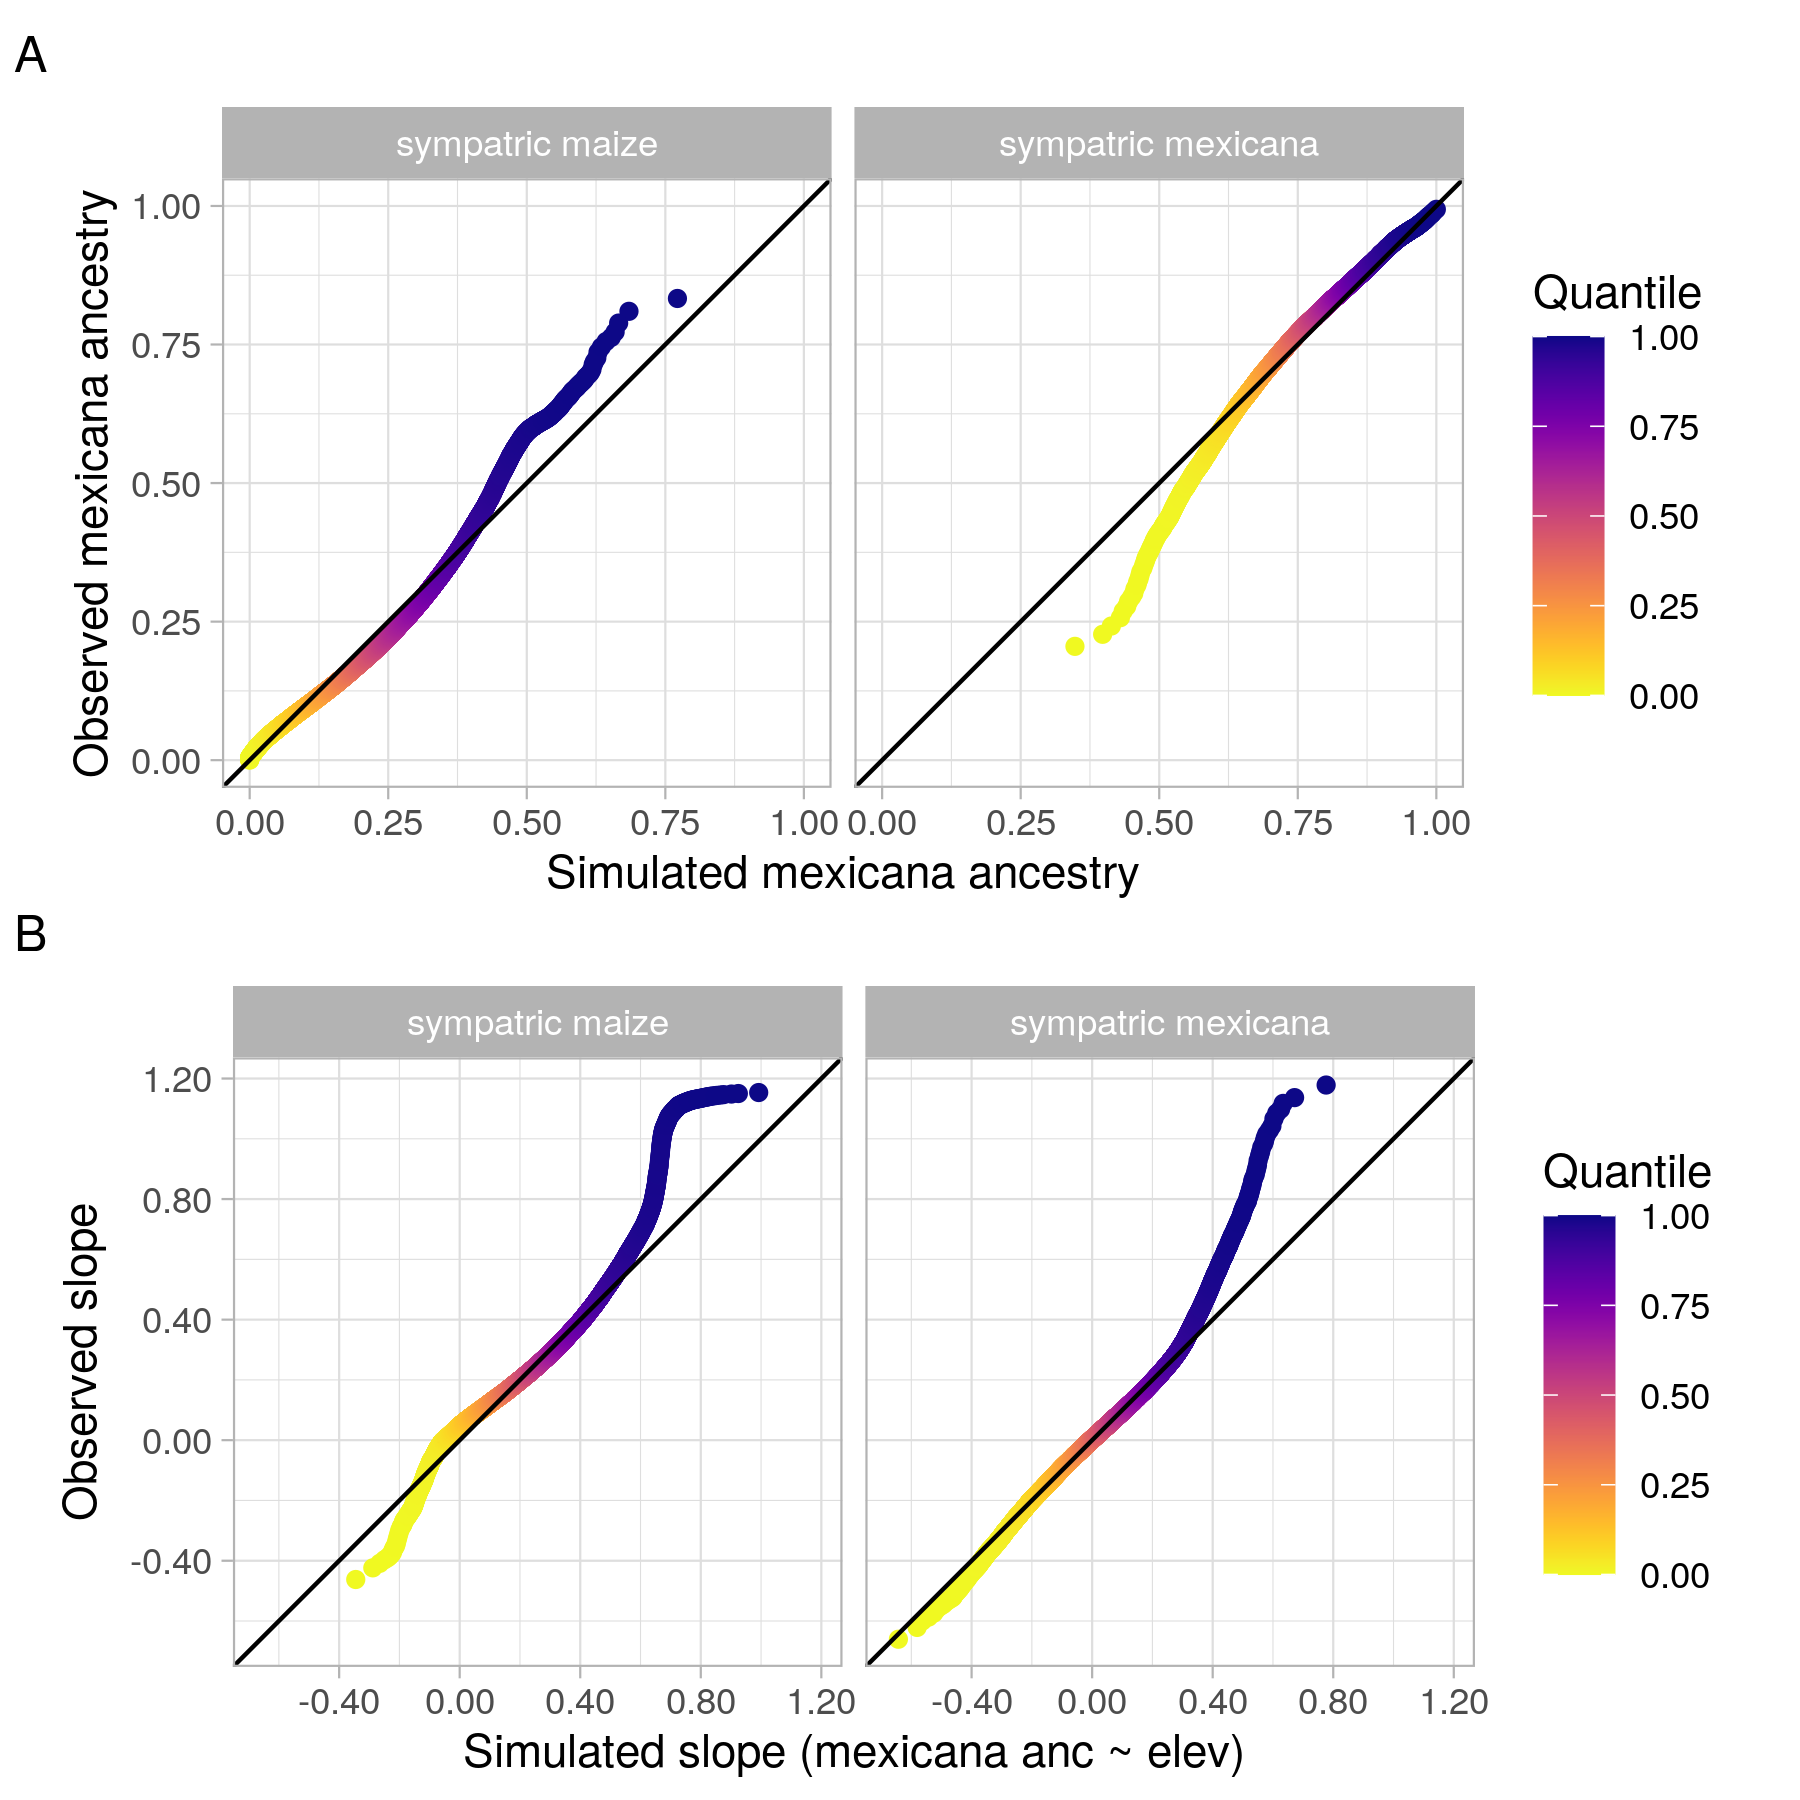
\includegraphics[width=\textwidth]{chapter2/figures/QQ.png}
\caption{\color{Gray} \textbf{Quantile comparison of observed data vs. MVN normal null model} (A) QQ-plot of simulated vs. observed mean ancestry at individual loci across all sympatric populations. (B) QQ-plot of simulated vs. observed slopes from the linear model \mexicana ancestry $\sim$ elevation at individual loci.}
\label{QQ}
\end{figure}

%\begin{figure}[p]
\begin{figure}[ht]
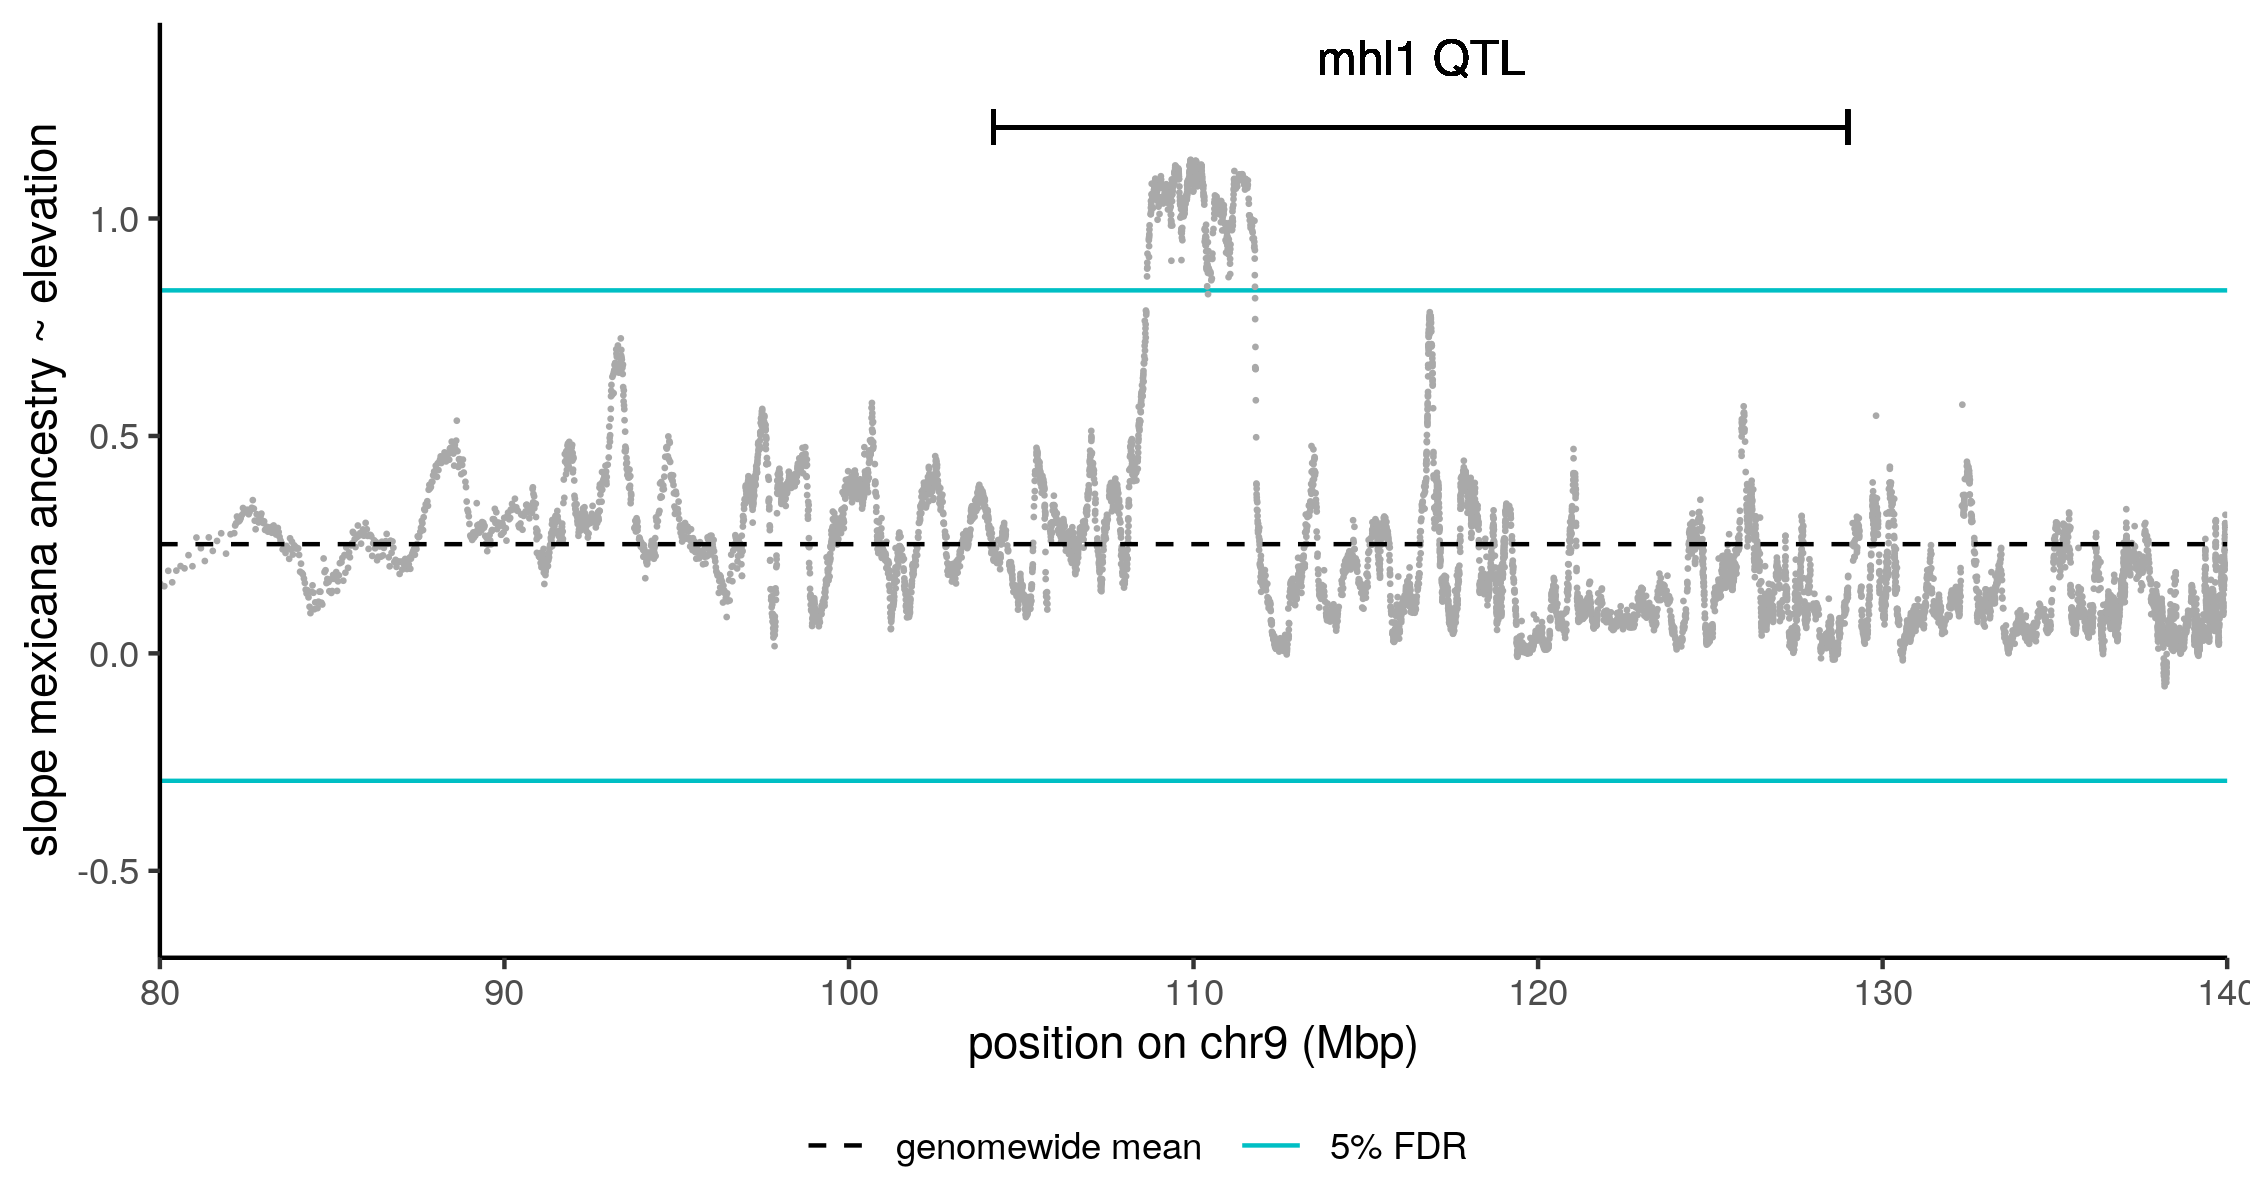
\includegraphics[width=\textwidth]{chapter2/figures/mhl1_inv_ancestry.png}
\caption{\color{Gray} \textbf{Ancestry slope with elevation at mhl1 locus}. Slope of introgressed \mexicana ancestry proportion in sympatric maize over a 1 km gain in elevation, zoomed in on the mhl1 QTL region on chromosome 9. Coordinates for the 3 Mb outlier region within this QTL are 9:108640415-111788150.}
\label{mhl1_slopes}
\end{figure}

%\begin{figure}[p]
\begin{figure}[ht]
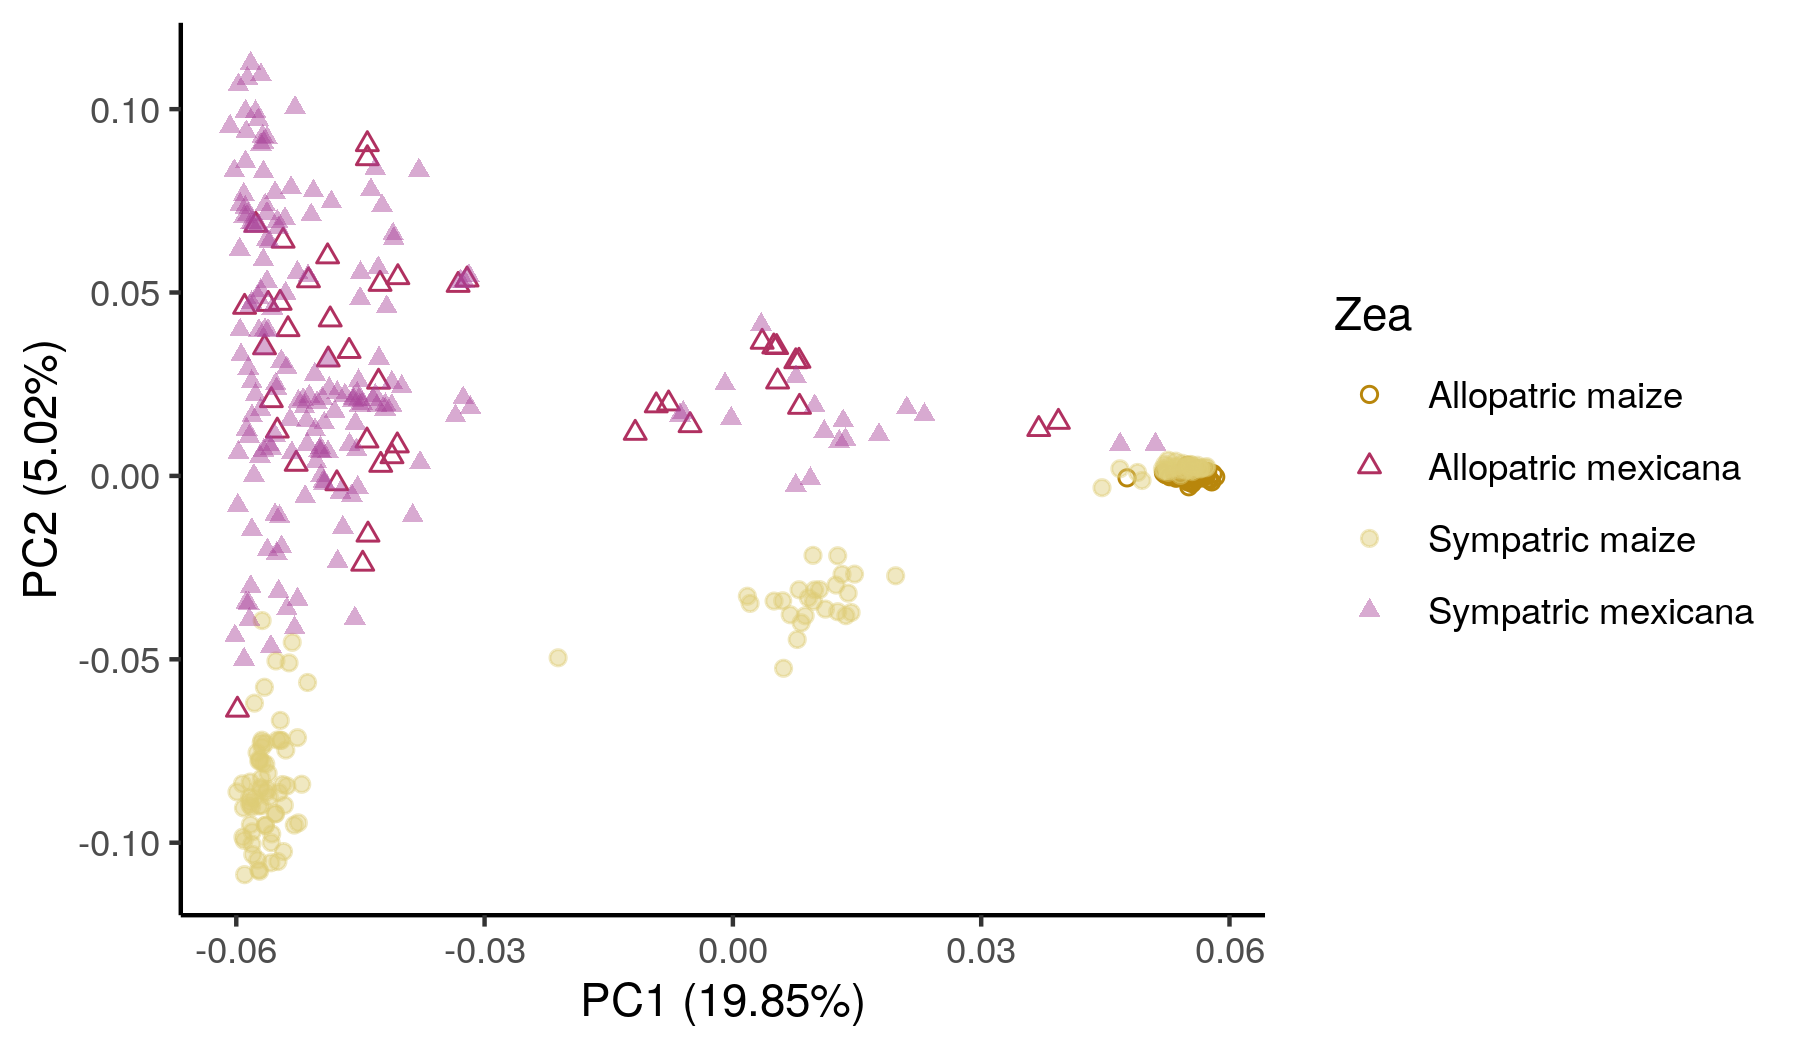
\includegraphics[width=\textwidth]{chapter2/figures/mhl1_inv_pca.png}
\caption{\color{Gray} \textbf{PCA of putative mhl1 inversion}. Principal components analysis of all SNPs in the 3 Mb outlier region within the mhl1 QTL region that shows a steep increase in introgressed \mexicana ancestry across elevation ($>$5\% FDR). This region on chromosome 9 is a putative inversion (9:108640415-111788150), separating out into three clusters across PC1: individuals homozygous for the common \mexicana inversion allele (left), heterozygous individuals (middle) and individuals homozygous for the common maize inversion allele (right; includes all allopatric \ec{reference} maize).}
\label{mhl1_pca}
\end{figure}

